\section{Testing}
With the theremin in a usable state, some testing was performed to assess the capabilities and extent to which the product would have to be improved or modified to allow it to be sold commercially. The main area that would need to be improved was the quality of the sound produced.

\subsection{Minimizing Interference}
In order to test the theremin quantitatively, a set-up was built such that no human variation could be included over the duration of the measurement. This involved making a second plate and grounding it to act as the user's hand such that it could be placed a a distant and would remain constant as opposed to a human user who's hand would move, obscuring the results. 

Using this apparatus, it was found that there was still a considerable amount of variation due to human interference simply because someone was near the wire that connected to the plate capacitor to the circuit. Because of the high frequencies involved, the effects of interference become amplified. This is basically the effect that was sought in order that the remote control be possible, but it has more of an effect than was expected on the rest of the circuit.

An attempt to reduce this noise was made using a coaxial cable to connect the plate capacitor and the circuit. Since the coaxial cable has an outer conducting layer, the field near the inner wire connecting the components is greatly reduced and so the interference from outside is also reduced. In order to reduce the effect still further, the distance between the circuit and capacitor could be reduced.

\subsection{Signal Variation}
A large contributing factor to the imperfections in the output signal is due to inaccuracies in the chip. These can be clearly seen in figure~\ref{fig:variations} where a series of measurements of the same signal are overlaid to show the differences. The measurements are of the same signal with no change, taken at 10\,second intervals.

\begin{figure}[htbp]
	\centering
		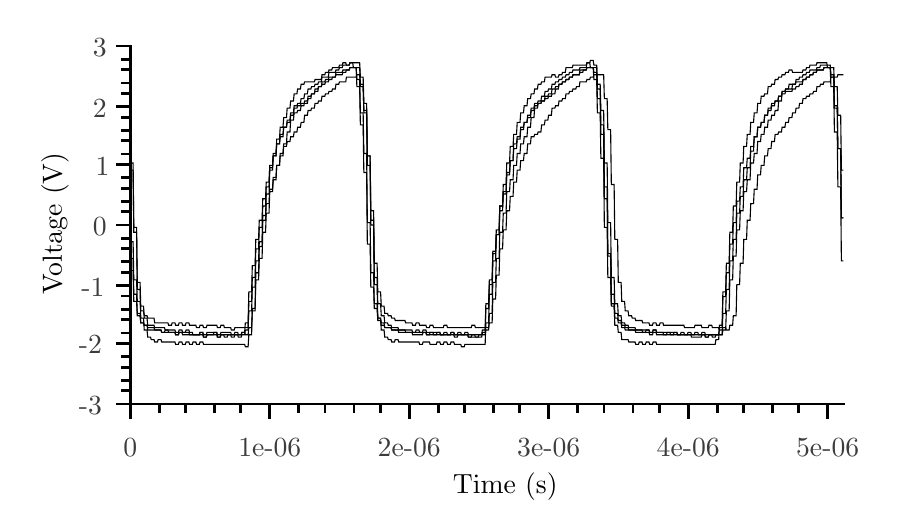
\begin{tikzpicture}{0pt}{0pt}{329pt}{180pt}
	\clip(0pt,180pt) -- (312.853pt,180pt) -- (312.853pt,8.83421pt) -- (0pt,8.83421pt) -- (0pt,180pt);
\begin{scope}
	\clip(37.0859pt,173.344pt) -- (294.786pt,173.344pt) -- (294.786pt,44.0183pt) -- (37.0859pt,44.0183pt) -- (37.0859pt,173.344pt);
	\color[gray]{0}
	\draw[line width=0.4pt, line join=miter, line cap=rect](37.3378pt,96.6106pt) -- (37.5897pt,96.6106pt) -- (37.8416pt,96.6106pt) -- (38.0935pt,96.6106pt) -- (38.3454pt,83.678pt) -- (38.5974pt,83.678pt) -- (38.8493pt,83.678pt) -- (39.1012pt,83.678pt) -- (39.3531pt,83.678pt) -- (39.605pt,76.7807pt) -- (39.8569pt,76.7807pt) -- (40.1088pt,76.7807pt) -- (40.3607pt,76.7807pt) -- (40.6126pt,76.7807pt) -- (40.8645pt,73.332pt) -- (41.1164pt,73.332pt) -- (41.3683pt,73.332pt) -- (41.6202pt,73.332pt) -- (41.8721pt,73.332pt) -- (42.124pt,72.4698pt) -- (42.3759pt,72.4698pt) -- (42.6278pt,72.4698pt) -- (42.8798pt,72.4698pt) -- (43.1317pt,72.4698pt) -- (43.3836pt,70.7455pt) -- (43.6355pt,70.7455pt) -- (43.8874pt,70.7455pt) -- (44.1393pt,70.7455pt) -- (44.3912pt,70.7455pt) -- (44.6431pt,70.7455pt) -- (44.895pt,70.7455pt) -- (45.1469pt,70.7455pt) -- (45.3988pt,70.7455pt) -- (45.6507pt,70.7455pt) -- (45.9026pt,70.7455pt) -- (46.1545pt,70.7455pt) -- (46.4064pt,70.7455pt) -- (46.6583pt,70.7455pt) -- (46.9102pt,70.7455pt) -- (47.1622pt,70.7455pt) -- (47.4141pt,70.7455pt) -- (47.666pt,70.7455pt) -- (47.9179pt,70.7455pt) -- (48.1698pt,70.7455pt) -- (48.4217pt,69.8833pt) -- (48.6736pt,69.8833pt) -- (48.9255pt,69.8833pt) -- (49.1774pt,69.8833pt) -- (49.4293pt,69.8833pt) -- (49.6812pt,69.8833pt) -- (49.9331pt,69.8833pt) -- (50.185pt,69.8833pt) -- (50.4369pt,69.8833pt) -- (50.6888pt,69.8833pt) -- (50.9407pt,69.8833pt) -- (51.1926pt,69.8833pt) -- (51.4446pt,69.8833pt) -- (51.6965pt,69.8833pt) -- (51.9484pt,69.8833pt) -- (52.2003pt,69.8833pt) -- (52.4522pt,69.8833pt) -- (52.7041pt,69.8833pt) -- (52.956pt,69.8833pt) -- (53.2079pt,69.8833pt) -- (53.4598pt,69.0212pt) -- (53.7117pt,69.0212pt) -- (53.9636pt,69.0212pt) -- (54.2155pt,69.0212pt) -- (54.4674pt,69.0212pt) -- (54.7193pt,69.8833pt) -- (54.9712pt,69.8833pt) -- (55.2231pt,69.8833pt) -- (55.475pt,69.8833pt) -- (55.7269pt,69.8833pt) -- (55.9789pt,69.0212pt) -- (56.2308pt,69.0212pt) -- (56.4827pt,69.0212pt) -- (56.7346pt,69.0212pt) -- (56.9865pt,69.0212pt) -- (57.2384pt,69.0212pt) -- (57.4903pt,69.0212pt) -- (57.7422pt,69.0212pt) -- (57.9941pt,69.0212pt) -- (58.246pt,69.0212pt) -- (58.4979pt,69.0212pt) -- (58.7498pt,69.0212pt) -- (59.0017pt,69.0212pt) -- (59.2536pt,69.0212pt) -- (59.5055pt,69.0212pt) -- (59.7574pt,69.0212pt) -- (60.0093pt,69.0212pt) -- (60.2613pt,69.0212pt) -- (60.5132pt,69.0212pt) -- (60.7651pt,69.0212pt) -- (61.017pt,69.0212pt) -- (61.2689pt,69.0212pt) -- (61.5208pt,69.0212pt) -- (61.7727pt,69.0212pt) -- (62.0246pt,69.0212pt) -- (62.2765pt,69.0212pt) -- (62.5284pt,69.0212pt) -- (62.7803pt,69.0212pt) -- (63.0322pt,69.0212pt) -- (63.2841pt,69.0212pt) -- (63.536pt,68.159pt) -- (63.7879pt,68.159pt) -- (64.0398pt,68.159pt) -- (64.2917pt,68.159pt) -- (64.5437pt,68.159pt) -- (64.7956pt,69.0212pt) -- (65.0475pt,69.0212pt) -- (65.2994pt,69.0212pt) -- (65.5513pt,69.0212pt) -- (65.8032pt,69.0212pt) -- (66.0551pt,69.0212pt) -- (66.307pt,69.0212pt) -- (66.5589pt,69.0212pt) -- (66.8108pt,69.0212pt) -- (67.0627pt,69.0212pt) -- (67.3146pt,69.0212pt) -- (67.5665pt,69.0212pt) -- (67.8184pt,69.0212pt) -- (68.0703pt,69.0212pt) -- (68.3222pt,69.0212pt) -- (68.5741pt,68.159pt) -- (68.826pt,68.159pt) -- (69.078pt,68.159pt) -- (69.3299pt,68.159pt) -- (69.5818pt,68.159pt) -- (69.8337pt,69.0212pt) -- (70.0856pt,69.0212pt) -- (70.3375pt,69.0212pt) -- (70.5894pt,69.0212pt) -- (70.8413pt,69.0212pt) -- (71.0932pt,68.159pt) -- (71.3451pt,68.159pt) -- (71.597pt,68.159pt) -- (71.8489pt,68.159pt) -- (72.1008pt,68.159pt) -- (72.3527pt,69.0212pt) -- (72.6046pt,69.0212pt) -- (72.8565pt,69.0212pt) -- (73.1084pt,69.0212pt) -- (73.3604pt,69.0212pt) -- (73.6123pt,68.159pt) -- (73.8642pt,68.159pt) -- (74.1161pt,68.159pt) -- (74.368pt,68.159pt) -- (74.6199pt,68.159pt) -- (74.8718pt,69.0212pt) -- (75.1237pt,69.0212pt) -- (75.3756pt,69.0212pt) -- (75.6275pt,69.0212pt) -- (75.8794pt,69.0212pt) -- (76.1313pt,68.159pt) -- (76.3832pt,68.159pt) -- (76.6351pt,68.159pt) -- (76.887pt,68.159pt) -- (77.1389pt,68.159pt) -- (77.3908pt,69.0212pt) -- (77.6428pt,69.0212pt) -- (77.8947pt,69.0212pt) -- (78.1466pt,69.0212pt) -- (78.3985pt,69.0212pt) -- (78.6504pt,70.7455pt) -- (78.9023pt,70.7455pt) -- (79.1542pt,70.7455pt) -- (79.4061pt,70.7455pt) -- (79.658pt,70.7455pt) -- (79.9099pt,81.0915pt) -- (80.1618pt,81.0915pt) -- (80.4137pt,81.0915pt) -- (80.6656pt,81.0915pt) -- (80.9175pt,81.0915pt) -- (81.1694pt,89.7132pt) -- (81.4213pt,89.7132pt) -- (81.6732pt,89.7132pt) -- (81.9251pt,89.7132pt) -- (82.1771pt,89.7132pt) -- (82.429pt,100.059pt) -- (82.6809pt,100.059pt) -- (82.9328pt,100.059pt) -- (83.1847pt,100.059pt) -- (83.4366pt,100.059pt) -- (83.6885pt,107.819pt) -- (83.9404pt,107.819pt) -- (84.1923pt,107.819pt) -- (84.4442pt,107.819pt) -- (84.6961pt,107.819pt) -- (84.948pt,115.578pt) -- (85.1999pt,115.578pt) -- (85.4518pt,115.578pt) -- (85.7037pt,115.578pt) -- (85.9556pt,115.578pt) -- (86.2075pt,122.476pt) -- (86.4595pt,122.476pt) -- (86.7114pt,122.476pt) -- (86.9633pt,122.476pt) -- (87.2152pt,122.476pt) -- (87.4671pt,130.235pt) -- (87.719pt,130.235pt) -- (87.9709pt,130.235pt) -- (88.2228pt,130.235pt) -- (88.4747pt,130.235pt) -- (88.7266pt,134.546pt) -- (88.9785pt,134.546pt) -- (89.2304pt,134.546pt) -- (89.4823pt,134.546pt) -- (89.7342pt,134.546pt) -- (89.9861pt,137.995pt) -- (90.238pt,137.995pt) -- (90.4899pt,137.995pt) -- (90.7419pt,137.995pt) -- (90.9938pt,137.995pt) -- (91.2457pt,141.443pt) -- (91.4976pt,141.443pt) -- (91.7495pt,141.443pt) -- (92.0014pt,141.443pt) -- (92.2533pt,141.443pt) -- (92.5052pt,144.03pt) -- (92.7571pt,144.03pt) -- (93.009pt,144.03pt) -- (93.2609pt,144.03pt) -- (93.5128pt,144.03pt) -- (93.7647pt,146.616pt) -- (94.0166pt,146.616pt) -- (94.2685pt,146.616pt) -- (94.5204pt,146.616pt) -- (94.7723pt,146.616pt) -- (95.0242pt,149.203pt) -- (95.2762pt,149.203pt) -- (95.5281pt,149.203pt) -- (95.78pt,149.203pt) -- (96.0319pt,149.203pt) -- (96.2838pt,151.789pt) -- (96.5357pt,151.789pt) -- (96.7876pt,151.789pt) -- (97.0395pt,151.789pt) -- (97.2914pt,151.789pt) -- (97.5433pt,152.652pt) -- (97.7952pt,152.652pt) -- (98.0471pt,152.652pt) -- (98.299pt,152.652pt) -- (98.5509pt,152.652pt) -- (98.8028pt,154.376pt) -- (99.0547pt,154.376pt) -- (99.3066pt,154.376pt) -- (99.5586pt,154.376pt) -- (99.8105pt,154.376pt) -- (100.062pt,156.1pt) -- (100.314pt,156.1pt) -- (100.566pt,156.1pt) -- (100.818pt,156.1pt) -- (101.07pt,156.1pt) -- (101.322pt,157.825pt) -- (101.574pt,157.825pt) -- (101.826pt,157.825pt) -- (102.078pt,157.825pt) -- (102.33pt,157.825pt) -- (102.581pt,158.687pt) -- (102.833pt,158.687pt) -- (103.085pt,158.687pt) -- (103.337pt,158.687pt) -- (103.589pt,158.687pt) -- (103.841pt,159.549pt) -- (104.093pt,159.549pt) -- (104.345pt,159.549pt) -- (104.597pt,159.549pt) -- (104.849pt,159.549pt) -- (105.1pt,160.411pt) -- (105.352pt,160.411pt) -- (105.604pt,160.411pt) -- (105.856pt,160.411pt) -- (106.108pt,160.411pt) -- (106.36pt,162.135pt) -- (106.612pt,162.135pt) -- (106.864pt,162.135pt) -- (107.116pt,162.135pt) -- (107.368pt,162.135pt) -- (107.62pt,162.135pt) -- (107.871pt,162.135pt) -- (108.123pt,162.135pt) -- (108.375pt,162.135pt) -- (108.627pt,162.135pt) -- (108.879pt,163.86pt) -- (109.131pt,163.86pt) -- (109.383pt,163.86pt) -- (109.635pt,163.86pt) -- (109.887pt,163.86pt) -- (110.139pt,163.86pt) -- (110.391pt,163.86pt) -- (110.642pt,163.86pt) -- (110.894pt,163.86pt) -- (111.146pt,163.86pt) -- (111.398pt,164.722pt) -- (111.65pt,164.722pt) -- (111.902pt,164.722pt) -- (112.154pt,164.722pt) -- (112.406pt,164.722pt) -- (112.658pt,165.584pt) -- (112.91pt,165.584pt) -- (113.161pt,165.584pt) -- (113.413pt,165.584pt) -- (113.665pt,165.584pt) -- (113.917pt,166.446pt) -- (114.169pt,166.446pt) -- (114.421pt,166.446pt) -- (114.673pt,166.446pt) -- (114.925pt,166.446pt) -- (115.177pt,166.446pt) -- (115.429pt,166.446pt) -- (115.681pt,166.446pt) -- (115.932pt,166.446pt) -- (116.184pt,166.446pt) -- (116.436pt,167.308pt) -- (116.688pt,167.308pt) -- (116.94pt,167.308pt) -- (117.192pt,167.308pt) -- (117.444pt,167.308pt) -- (117.696pt,165.584pt) -- (117.948pt,165.584pt) -- (118.2pt,165.584pt) -- (118.451pt,165.584pt) -- (118.703pt,165.584pt) -- (118.955pt,158.687pt) -- (119.207pt,158.687pt) -- (119.459pt,158.687pt) -- (119.711pt,158.687pt) -- (119.963pt,158.687pt) -- (120.215pt,144.892pt) -- (120.467pt,144.892pt) -- (120.719pt,144.892pt) -- (120.971pt,144.892pt) -- (121.222pt,144.892pt) -- (121.474pt,127.649pt) -- (121.726pt,127.649pt) -- (121.978pt,127.649pt) -- (122.23pt,127.649pt) -- (122.482pt,127.649pt) -- (122.734pt,101.784pt) -- (122.986pt,101.784pt) -- (123.238pt,101.784pt) -- (123.49pt,101.784pt) -- (123.742pt,101.784pt) -- (123.993pt,86.2645pt) -- (124.245pt,86.2645pt) -- (124.497pt,86.2645pt) -- (124.749pt,86.2645pt) -- (125.001pt,86.2645pt) -- (125.253pt,78.505pt) -- (125.505pt,78.505pt) -- (125.757pt,78.505pt) -- (126.009pt,78.505pt) -- (126.261pt,78.505pt) -- (126.512pt,74.1942pt) -- (126.764pt,74.1942pt) -- (127.016pt,74.1942pt) -- (127.268pt,74.1942pt) -- (127.52pt,74.1942pt) -- (127.772pt,72.4698pt) -- (128.024pt,72.4698pt) -- (128.276pt,72.4698pt) -- (128.528pt,72.4698pt) -- (128.78pt,72.4698pt) -- (129.032pt,71.6077pt) -- (129.283pt,71.6077pt) -- (129.535pt,71.6077pt) -- (129.787pt,71.6077pt) -- (130.039pt,71.6077pt) -- (130.291pt,71.6077pt) -- (130.543pt,71.6077pt) -- (130.795pt,71.6077pt) -- (131.047pt,71.6077pt) -- (131.299pt,71.6077pt) -- (131.551pt,70.7455pt) -- (131.802pt,70.7455pt) -- (132.054pt,70.7455pt) -- (132.306pt,70.7455pt) -- (132.558pt,70.7455pt) -- (132.81pt,70.7455pt) -- (133.062pt,70.7455pt) -- (133.314pt,70.7455pt) -- (133.566pt,70.7455pt) -- (133.818pt,70.7455pt) -- (134.07pt,69.8833pt) -- (134.322pt,69.8833pt) -- (134.573pt,69.8833pt) -- (134.825pt,69.8833pt) -- (135.077pt,69.8833pt) -- (135.329pt,69.8833pt) -- (135.581pt,69.8833pt) -- (135.833pt,69.8833pt) -- (136.085pt,69.8833pt) -- (136.337pt,69.8833pt) -- (136.589pt,69.8833pt) -- (136.841pt,69.8833pt) -- (137.093pt,69.8833pt) -- (137.344pt,69.8833pt) -- (137.596pt,69.8833pt) -- (137.848pt,69.8833pt) -- (138.1pt,69.8833pt) -- (138.352pt,69.8833pt) -- (138.604pt,69.8833pt) -- (138.856pt,69.8833pt) -- (139.108pt,69.0212pt) -- (139.36pt,69.0212pt) -- (139.612pt,69.0212pt) -- (139.863pt,69.0212pt) -- (140.115pt,69.0212pt) -- (140.367pt,69.0212pt) -- (140.619pt,69.0212pt) -- (140.871pt,69.0212pt) -- (141.123pt,69.0212pt) -- (141.375pt,69.0212pt) -- (141.627pt,69.0212pt) -- (141.879pt,69.0212pt) -- (142.131pt,69.0212pt) -- (142.383pt,69.0212pt) -- (142.634pt,69.0212pt) -- (142.886pt,69.8833pt) -- (143.138pt,69.8833pt) -- (143.39pt,69.8833pt) -- (143.642pt,69.8833pt) -- (143.894pt,69.8833pt) -- (144.146pt,69.0212pt) -- (144.398pt,69.0212pt) -- (144.65pt,69.0212pt) -- (144.902pt,69.0212pt) -- (145.153pt,69.0212pt) -- (145.405pt,69.0212pt) -- (145.657pt,69.0212pt) -- (145.909pt,69.0212pt) -- (146.161pt,69.0212pt) -- (146.413pt,69.0212pt) -- (146.665pt,69.0212pt) -- (146.917pt,69.0212pt) -- (147.169pt,69.0212pt) -- (147.421pt,69.0212pt) -- (147.673pt,69.0212pt) -- (147.924pt,69.0212pt) -- (148.176pt,69.0212pt) -- (148.428pt,69.0212pt) -- (148.68pt,69.0212pt) -- (148.932pt,69.0212pt) -- (149.184pt,69.0212pt) -- (149.436pt,69.0212pt) -- (149.688pt,69.0212pt) -- (149.94pt,69.0212pt) -- (150.192pt,69.0212pt) -- (150.444pt,69.0212pt) -- (150.695pt,69.0212pt) -- (150.947pt,69.0212pt) -- (151.199pt,69.0212pt) -- (151.451pt,69.0212pt) -- (151.703pt,69.0212pt) -- (151.955pt,69.0212pt) -- (152.207pt,69.0212pt) -- (152.459pt,69.0212pt) -- (152.711pt,69.0212pt) -- (152.963pt,69.0212pt) -- (153.214pt,69.0212pt) -- (153.466pt,69.0212pt) -- (153.718pt,69.0212pt) -- (153.97pt,69.0212pt) -- (154.222pt,68.159pt) -- (154.474pt,68.159pt) -- (154.726pt,68.159pt) -- (154.978pt,68.159pt) -- (155.23pt,68.159pt) -- (155.482pt,69.0212pt) -- (155.734pt,69.0212pt) -- (155.985pt,69.0212pt) -- (156.237pt,69.0212pt) -- (156.489pt,69.0212pt) -- (156.741pt,69.0212pt) -- (156.993pt,69.0212pt) -- (157.245pt,69.0212pt) -- (157.497pt,69.0212pt) -- (157.749pt,69.0212pt) -- (158.001pt,69.0212pt) -- (158.253pt,69.0212pt) -- (158.505pt,69.0212pt) -- (158.756pt,69.0212pt) -- (159.008pt,69.0212pt) -- (159.26pt,68.159pt) -- (159.512pt,68.159pt) -- (159.764pt,68.159pt) -- (160.016pt,68.159pt) -- (160.268pt,68.159pt) -- (160.52pt,68.159pt) -- (160.772pt,68.159pt) -- (161.024pt,68.159pt) -- (161.275pt,68.159pt) -- (161.527pt,68.159pt) -- (161.779pt,68.159pt) -- (162.031pt,68.159pt) -- (162.283pt,68.159pt) -- (162.535pt,68.159pt) -- (162.787pt,68.159pt) -- (163.039pt,68.159pt) -- (163.291pt,68.159pt) -- (163.543pt,68.159pt) -- (163.795pt,68.159pt) -- (164.046pt,68.159pt) -- (164.298pt,69.8833pt) -- (164.55pt,69.8833pt) -- (164.802pt,69.8833pt) -- (165.054pt,69.8833pt) -- (165.306pt,69.8833pt) -- (165.558pt,78.505pt) -- (165.81pt,78.505pt) -- (166.062pt,78.505pt) -- (166.314pt,78.505pt) -- (166.565pt,78.505pt) -- (166.817pt,87.1267pt) -- (167.069pt,87.1267pt) -- (167.321pt,87.1267pt) -- (167.573pt,87.1267pt) -- (167.825pt,87.1267pt) -- (168.077pt,98.3349pt) -- (168.329pt,98.3349pt) -- (168.581pt,98.3349pt) -- (168.833pt,98.3349pt) -- (169.085pt,98.3349pt) -- (169.336pt,105.232pt) -- (169.588pt,105.232pt) -- (169.84pt,105.232pt) -- (170.092pt,105.232pt) -- (170.344pt,105.232pt) -- (170.596pt,113.854pt) -- (170.848pt,113.854pt) -- (171.1pt,113.854pt) -- (171.352pt,113.854pt) -- (171.604pt,113.854pt) -- (171.856pt,119.889pt) -- (172.107pt,119.889pt) -- (172.359pt,119.889pt) -- (172.611pt,119.889pt) -- (172.863pt,119.889pt) -- (173.115pt,126.786pt) -- (173.367pt,126.786pt) -- (173.619pt,126.786pt) -- (173.871pt,126.786pt) -- (174.123pt,126.786pt) -- (174.375pt,131.959pt) -- (174.626pt,131.959pt) -- (174.878pt,131.959pt) -- (175.13pt,131.959pt) -- (175.382pt,131.959pt) -- (175.634pt,137.995pt) -- (175.886pt,137.995pt) -- (176.138pt,137.995pt) -- (176.39pt,137.995pt) -- (176.642pt,137.995pt) -- (176.894pt,140.581pt) -- (177.146pt,140.581pt) -- (177.397pt,140.581pt) -- (177.649pt,140.581pt) -- (177.901pt,140.581pt) -- (178.153pt,144.03pt) -- (178.405pt,144.03pt) -- (178.657pt,144.03pt) -- (178.909pt,144.03pt) -- (179.161pt,144.03pt) -- (179.413pt,145.754pt) -- (179.665pt,145.754pt) -- (179.916pt,145.754pt) -- (180.168pt,145.754pt) -- (180.42pt,145.754pt) -- (180.672pt,148.341pt) -- (180.924pt,148.341pt) -- (181.176pt,148.341pt) -- (181.428pt,148.341pt) -- (181.68pt,148.341pt) -- (181.932pt,150.927pt) -- (182.184pt,150.927pt) -- (182.436pt,150.927pt) -- (182.687pt,150.927pt) -- (182.939pt,150.927pt) -- (183.191pt,152.652pt) -- (183.443pt,152.652pt) -- (183.695pt,152.652pt) -- (183.947pt,152.652pt) -- (184.199pt,152.652pt) -- (184.451pt,153.514pt) -- (184.703pt,153.514pt) -- (184.955pt,153.514pt) -- (185.207pt,153.514pt) -- (185.458pt,153.514pt) -- (185.71pt,155.238pt) -- (185.962pt,155.238pt) -- (186.214pt,155.238pt) -- (186.466pt,155.238pt) -- (186.718pt,155.238pt) -- (186.97pt,156.962pt) -- (187.222pt,156.962pt) -- (187.474pt,156.962pt) -- (187.726pt,156.962pt) -- (187.977pt,156.962pt) -- (188.229pt,157.825pt) -- (188.481pt,157.825pt) -- (188.733pt,157.825pt) -- (188.985pt,157.825pt) -- (189.237pt,157.825pt) -- (189.489pt,159.549pt) -- (189.741pt,159.549pt) -- (189.993pt,159.549pt) -- (190.245pt,159.549pt) -- (190.497pt,159.549pt) -- (190.748pt,160.411pt) -- (191pt,160.411pt) -- (191.252pt,160.411pt) -- (191.504pt,160.411pt) -- (191.756pt,160.411pt) -- (192.008pt,161.273pt) -- (192.26pt,161.273pt) -- (192.512pt,161.273pt) -- (192.764pt,161.273pt) -- (193.016pt,161.273pt) -- (193.267pt,162.135pt) -- (193.519pt,162.135pt) -- (193.771pt,162.135pt) -- (194.023pt,162.135pt) -- (194.275pt,162.135pt) -- (194.527pt,162.998pt) -- (194.779pt,162.998pt) -- (195.031pt,162.998pt) -- (195.283pt,162.998pt) -- (195.535pt,162.998pt) -- (195.787pt,163.86pt) -- (196.038pt,163.86pt) -- (196.29pt,163.86pt) -- (196.542pt,163.86pt) -- (196.794pt,163.86pt) -- (197.046pt,164.722pt) -- (197.298pt,164.722pt) -- (197.55pt,164.722pt) -- (197.802pt,164.722pt) -- (198.054pt,164.722pt) -- (198.306pt,164.722pt) -- (198.558pt,164.722pt) -- (198.809pt,164.722pt) -- (199.061pt,164.722pt) -- (199.313pt,164.722pt) -- (199.565pt,165.584pt) -- (199.817pt,165.584pt) -- (200.069pt,165.584pt) -- (200.321pt,165.584pt) -- (200.573pt,165.584pt) -- (200.825pt,165.584pt) -- (201.077pt,165.584pt) -- (201.328pt,165.584pt) -- (201.58pt,165.584pt) -- (201.832pt,165.584pt) -- (202.084pt,167.308pt) -- (202.336pt,167.308pt) -- (202.588pt,167.308pt) -- (202.84pt,167.308pt) -- (203.092pt,167.308pt) -- (203.344pt,165.584pt) -- (203.596pt,165.584pt) -- (203.848pt,165.584pt) -- (204.099pt,165.584pt) -- (204.351pt,165.584pt) -- (204.603pt,161.273pt) -- (204.855pt,161.273pt) -- (205.107pt,161.273pt) -- (205.359pt,161.273pt) -- (205.611pt,161.273pt) -- (205.863pt,149.203pt) -- (206.115pt,149.203pt) -- (206.367pt,149.203pt) -- (206.619pt,149.203pt) -- (206.87pt,149.203pt) -- (207.122pt,132.822pt) -- (207.374pt,132.822pt) -- (207.626pt,132.822pt) -- (207.878pt,132.822pt) -- (208.13pt,132.822pt) -- (208.382pt,107.819pt) -- (208.634pt,107.819pt) -- (208.886pt,107.819pt) -- (209.138pt,107.819pt) -- (209.389pt,107.819pt) -- (209.641pt,89.7132pt) -- (209.893pt,89.7132pt) -- (210.145pt,89.7132pt) -- (210.397pt,89.7132pt) -- (210.649pt,89.7132pt) -- (210.901pt,79.3672pt) -- (211.153pt,79.3672pt) -- (211.405pt,79.3672pt) -- (211.657pt,79.3672pt) -- (211.909pt,79.3672pt) -- (212.16pt,75.0564pt) -- (212.412pt,75.0564pt) -- (212.664pt,75.0564pt) -- (212.916pt,75.0564pt) -- (213.168pt,75.0564pt) -- (213.42pt,73.332pt) -- (213.672pt,73.332pt) -- (213.924pt,73.332pt) -- (214.176pt,73.332pt) -- (214.428pt,73.332pt) -- (214.679pt,71.6077pt) -- (214.931pt,71.6077pt) -- (215.183pt,71.6077pt) -- (215.435pt,71.6077pt) -- (215.687pt,71.6077pt) -- (215.939pt,70.7455pt) -- (216.191pt,70.7455pt) -- (216.443pt,70.7455pt) -- (216.695pt,70.7455pt) -- (216.947pt,70.7455pt) -- (217.199pt,70.7455pt) -- (217.45pt,70.7455pt) -- (217.702pt,70.7455pt) -- (217.954pt,70.7455pt) -- (218.206pt,70.7455pt) -- (218.458pt,70.7455pt) -- (218.71pt,70.7455pt) -- (218.962pt,70.7455pt) -- (219.214pt,70.7455pt) -- (219.466pt,70.7455pt) -- (219.718pt,69.8833pt) -- (219.97pt,69.8833pt) -- (220.221pt,69.8833pt) -- (220.473pt,69.8833pt) -- (220.725pt,69.8833pt) -- (220.977pt,69.8833pt) -- (221.229pt,69.8833pt) -- (221.481pt,69.8833pt) -- (221.733pt,69.8833pt) -- (221.985pt,69.8833pt) -- (222.237pt,69.8833pt) -- (222.489pt,69.8833pt) -- (222.74pt,69.8833pt) -- (222.992pt,69.8833pt) -- (223.244pt,69.8833pt) -- (223.496pt,69.8833pt) -- (223.748pt,69.8833pt) -- (224pt,69.8833pt) -- (224.252pt,69.8833pt) -- (224.504pt,69.8833pt) -- (224.756pt,69.0212pt) -- (225.008pt,69.0212pt) -- (225.26pt,69.0212pt) -- (225.511pt,69.0212pt) -- (225.763pt,69.0212pt) -- (226.015pt,69.8833pt) -- (226.267pt,69.8833pt) -- (226.519pt,69.8833pt) -- (226.771pt,69.8833pt) -- (227.023pt,69.8833pt) -- (227.275pt,69.0212pt) -- (227.527pt,69.0212pt) -- (227.779pt,69.0212pt) -- (228.03pt,69.0212pt) -- (228.282pt,69.0212pt) -- (228.534pt,69.0212pt) -- (228.786pt,69.0212pt) -- (229.038pt,69.0212pt) -- (229.29pt,69.0212pt) -- (229.542pt,69.0212pt) -- (229.794pt,69.0212pt) -- (230.046pt,69.0212pt) -- (230.298pt,69.0212pt) -- (230.55pt,69.0212pt) -- (230.801pt,69.0212pt) -- (231.053pt,69.0212pt) -- (231.305pt,69.0212pt) -- (231.557pt,69.0212pt) -- (231.809pt,69.0212pt) -- (232.061pt,69.0212pt) -- (232.313pt,69.0212pt) -- (232.565pt,69.0212pt) -- (232.817pt,69.0212pt) -- (233.069pt,69.0212pt) -- (233.321pt,69.0212pt) -- (233.572pt,69.0212pt) -- (233.824pt,69.0212pt) -- (234.076pt,69.0212pt) -- (234.328pt,69.0212pt) -- (234.58pt,69.0212pt) -- (234.832pt,69.0212pt) -- (235.084pt,69.0212pt) -- (235.336pt,69.0212pt) -- (235.588pt,69.0212pt) -- (235.84pt,69.0212pt) -- (236.091pt,69.0212pt) -- (236.343pt,69.0212pt) -- (236.595pt,69.0212pt) -- (236.847pt,69.0212pt) -- (237.099pt,69.0212pt) -- (237.351pt,69.0212pt) -- (237.603pt,69.0212pt) -- (237.855pt,69.0212pt) -- (238.107pt,69.0212pt) -- (238.359pt,69.0212pt) -- (238.611pt,69.0212pt) -- (238.862pt,69.0212pt) -- (239.114pt,69.0212pt) -- (239.366pt,69.0212pt) -- (239.618pt,69.0212pt) -- (239.87pt,68.159pt) -- (240.122pt,68.159pt) -- (240.374pt,68.159pt) -- (240.626pt,68.159pt) -- (240.878pt,68.159pt) -- (241.13pt,68.159pt) -- (241.382pt,68.159pt) -- (241.633pt,68.159pt) -- (241.885pt,68.159pt) -- (242.137pt,68.159pt) -- (242.389pt,68.159pt) -- (242.641pt,68.159pt) -- (242.893pt,68.159pt) -- (243.145pt,68.159pt) -- (243.397pt,68.159pt) -- (243.649pt,69.0212pt) -- (243.901pt,69.0212pt) -- (244.152pt,69.0212pt) -- (244.404pt,69.0212pt) -- (244.656pt,69.0212pt) -- (244.908pt,68.159pt) -- (245.16pt,68.159pt) -- (245.412pt,68.159pt) -- (245.664pt,68.159pt) -- (245.916pt,68.159pt) -- (246.168pt,69.0212pt) -- (246.42pt,69.0212pt) -- (246.672pt,69.0212pt) -- (246.923pt,69.0212pt) -- (247.175pt,69.0212pt) -- (247.427pt,68.159pt) -- (247.679pt,68.159pt) -- (247.931pt,68.159pt) -- (248.183pt,68.159pt) -- (248.435pt,68.159pt) -- (248.687pt,69.0212pt) -- (248.939pt,69.0212pt) -- (249.191pt,69.0212pt) -- (249.442pt,69.0212pt) -- (249.694pt,69.0212pt) -- (249.946pt,69.0212pt) -- (250.198pt,69.0212pt) -- (250.45pt,69.0212pt) -- (250.702pt,69.0212pt) -- (250.954pt,69.0212pt) -- (251.206pt,76.7807pt) -- (251.458pt,76.7807pt) -- (251.71pt,76.7807pt) -- (251.962pt,76.7807pt) -- (252.213pt,76.7807pt) -- (252.465pt,85.4024pt) -- (252.717pt,85.4024pt) -- (252.969pt,85.4024pt) -- (253.221pt,85.4024pt) -- (253.473pt,85.4024pt) -- (253.725pt,95.7484pt) -- (253.977pt,95.7484pt) -- (254.229pt,95.7484pt) -- (254.481pt,95.7484pt) -- (254.733pt,95.7484pt) -- (254.984pt,103.508pt) -- (255.236pt,103.508pt) -- (255.488pt,103.508pt) -- (255.74pt,103.508pt) -- (255.992pt,103.508pt) -- (256.244pt,112.992pt) -- (256.496pt,112.992pt) -- (256.748pt,112.992pt) -- (257pt,112.992pt) -- (257.252pt,112.992pt) -- (257.503pt,119.027pt) -- (257.755pt,119.027pt) -- (258.007pt,119.027pt) -- (258.259pt,119.027pt) -- (258.511pt,119.027pt) -- (258.763pt,125.062pt) -- (259.015pt,125.062pt) -- (259.267pt,125.062pt) -- (259.519pt,125.062pt) -- (259.771pt,125.062pt) -- (260.023pt,129.373pt) -- (260.274pt,129.373pt) -- (260.526pt,129.373pt) -- (260.778pt,129.373pt) -- (261.03pt,129.373pt) -- (261.282pt,135.408pt) -- (261.534pt,135.408pt) -- (261.786pt,135.408pt) -- (262.038pt,135.408pt) -- (262.29pt,135.408pt) -- (262.542pt,140.581pt) -- (262.793pt,140.581pt) -- (263.045pt,140.581pt) -- (263.297pt,140.581pt) -- (263.549pt,140.581pt) -- (263.801pt,144.03pt) -- (264.053pt,144.03pt) -- (264.305pt,144.03pt) -- (264.557pt,144.03pt) -- (264.809pt,144.03pt) -- (265.061pt,145.754pt) -- (265.313pt,145.754pt) -- (265.564pt,145.754pt) -- (265.816pt,145.754pt) -- (266.068pt,145.754pt) -- (266.32pt,148.341pt) -- (266.572pt,148.341pt) -- (266.824pt,148.341pt) -- (267.076pt,148.341pt) -- (267.328pt,148.341pt) -- (267.58pt,150.065pt) -- (267.832pt,150.065pt) -- (268.084pt,150.065pt) -- (268.335pt,150.065pt) -- (268.587pt,150.065pt) -- (268.839pt,151.789pt) -- (269.091pt,151.789pt) -- (269.343pt,151.789pt) -- (269.595pt,151.789pt) -- (269.847pt,151.789pt) -- (270.099pt,153.514pt) -- (270.351pt,153.514pt) -- (270.603pt,153.514pt) -- (270.854pt,153.514pt) -- (271.106pt,153.514pt) -- (271.358pt,155.238pt) -- (271.61pt,155.238pt) -- (271.862pt,155.238pt) -- (272.114pt,155.238pt) -- (272.366pt,155.238pt) -- (272.618pt,156.962pt) -- (272.87pt,156.962pt) -- (273.122pt,156.962pt) -- (273.374pt,156.962pt) -- (273.625pt,156.962pt) -- (273.877pt,157.825pt) -- (274.129pt,157.825pt) -- (274.381pt,157.825pt) -- (274.633pt,157.825pt) -- (274.885pt,157.825pt) -- (275.137pt,159.549pt) -- (275.389pt,159.549pt) -- (275.641pt,159.549pt) -- (275.893pt,159.549pt) -- (276.144pt,159.549pt) -- (276.396pt,159.549pt) -- (276.648pt,159.549pt) -- (276.9pt,159.549pt) -- (277.152pt,159.549pt) -- (277.404pt,159.549pt) -- (277.656pt,161.273pt) -- (277.908pt,161.273pt) -- (278.16pt,161.273pt) -- (278.412pt,161.273pt) -- (278.664pt,161.273pt) -- (278.915pt,162.135pt) -- (279.167pt,162.135pt) -- (279.419pt,162.135pt) -- (279.671pt,162.135pt) -- (279.923pt,162.135pt) -- (280.175pt,162.998pt) -- (280.427pt,162.998pt) -- (280.679pt,162.998pt) -- (280.931pt,162.998pt) -- (281.183pt,162.998pt) -- (281.435pt,163.86pt) -- (281.686pt,163.86pt) -- (281.938pt,163.86pt) -- (282.19pt,163.86pt) -- (282.442pt,163.86pt) -- (282.694pt,164.722pt) -- (282.946pt,164.722pt) -- (283.198pt,164.722pt) -- (283.45pt,164.722pt) -- (283.702pt,164.722pt) -- (283.954pt,164.722pt) -- (284.205pt,164.722pt) -- (284.457pt,164.722pt) -- (284.709pt,164.722pt) -- (284.961pt,164.722pt) -- (285.213pt,165.584pt) -- (285.465pt,165.584pt) -- (285.717pt,165.584pt) -- (285.969pt,165.584pt) -- (286.221pt,165.584pt) -- (286.473pt,166.446pt) -- (286.725pt,166.446pt) -- (286.976pt,166.446pt) -- (287.228pt,166.446pt) -- (287.48pt,166.446pt) -- (287.732pt,166.446pt) -- (287.984pt,166.446pt) -- (288.236pt,166.446pt) -- (288.488pt,166.446pt) -- (288.74pt,166.446pt) -- (288.992pt,166.446pt) -- (289.244pt,166.446pt) -- (289.496pt,166.446pt) -- (289.747pt,166.446pt) -- (289.999pt,166.446pt) -- (290.251pt,162.998pt) -- (290.503pt,162.998pt) -- (290.755pt,162.998pt) -- (291.007pt,162.998pt) -- (291.259pt,162.998pt) -- (291.511pt,151.789pt) -- (291.763pt,151.789pt) -- (292.015pt,151.789pt) -- (292.266pt,151.789pt) -- (292.518pt,151.789pt) -- (292.77pt,136.27pt) -- (293.022pt,136.27pt) -- (293.274pt,136.27pt) -- (293.526pt,136.27pt) -- (293.778pt,136.27pt) -- (294.03pt,111.267pt) -- (294.282pt,111.267pt) -- (294.534pt,111.267pt) -- (294.786pt,111.267pt);
	\color[gray]{0}
	\draw[line width=0.4pt, line join=miter, line cap=rect](37.3378pt,92.2997pt) -- (37.5897pt,92.2997pt) -- (37.8416pt,92.2997pt) -- (38.0935pt,92.2997pt) -- (38.3454pt,81.0915pt) -- (38.5974pt,81.0915pt) -- (38.8493pt,81.0915pt) -- (39.1012pt,81.0915pt) -- (39.3531pt,81.0915pt) -- (39.605pt,75.9185pt) -- (39.8569pt,75.9185pt) -- (40.1088pt,75.9185pt) -- (40.3607pt,75.9185pt) -- (40.6126pt,75.9185pt) -- (40.8645pt,73.332pt) -- (41.1164pt,73.332pt) -- (41.3683pt,73.332pt) -- (41.6202pt,73.332pt) -- (41.8721pt,73.332pt) -- (42.124pt,72.4698pt) -- (42.3759pt,72.4698pt) -- (42.6278pt,72.4698pt) -- (42.8798pt,72.4698pt) -- (43.1317pt,72.4698pt) -- (43.3836pt,71.6077pt) -- (43.6355pt,71.6077pt) -- (43.8874pt,71.6077pt) -- (44.1393pt,71.6077pt) -- (44.3912pt,71.6077pt) -- (44.6431pt,71.6077pt) -- (44.895pt,71.6077pt) -- (45.1469pt,71.6077pt) -- (45.3988pt,71.6077pt) -- (45.6507pt,71.6077pt) -- (45.9026pt,70.7455pt) -- (46.1545pt,70.7455pt) -- (46.4064pt,70.7455pt) -- (46.6583pt,70.7455pt) -- (46.9102pt,70.7455pt) -- (47.1622pt,70.7455pt) -- (47.4141pt,70.7455pt) -- (47.666pt,70.7455pt) -- (47.9179pt,70.7455pt) -- (48.1698pt,70.7455pt) -- (48.4217pt,69.8833pt) -- (48.6736pt,69.8833pt) -- (48.9255pt,69.8833pt) -- (49.1774pt,69.8833pt) -- (49.4293pt,69.8833pt) -- (49.6812pt,70.7455pt) -- (49.9331pt,70.7455pt) -- (50.185pt,70.7455pt) -- (50.4369pt,70.7455pt) -- (50.6888pt,70.7455pt) -- (50.9407pt,69.8833pt) -- (51.1926pt,69.8833pt) -- (51.4446pt,69.8833pt) -- (51.6965pt,69.8833pt) -- (51.9484pt,69.8833pt) -- (52.2003pt,69.8833pt) -- (52.4522pt,69.8833pt) -- (52.7041pt,69.8833pt) -- (52.956pt,69.8833pt) -- (53.2079pt,69.8833pt) -- (53.4598pt,69.0212pt) -- (53.7117pt,69.0212pt) -- (53.9636pt,69.0212pt) -- (54.2155pt,69.0212pt) -- (54.4674pt,69.0212pt) -- (54.7193pt,69.8833pt) -- (54.9712pt,69.8833pt) -- (55.2231pt,69.8833pt) -- (55.475pt,69.8833pt) -- (55.7269pt,69.8833pt) -- (55.9789pt,69.8833pt) -- (56.2308pt,69.8833pt) -- (56.4827pt,69.8833pt) -- (56.7346pt,69.8833pt) -- (56.9865pt,69.8833pt) -- (57.2384pt,69.8833pt) -- (57.4903pt,69.8833pt) -- (57.7422pt,69.8833pt) -- (57.9941pt,69.8833pt) -- (58.246pt,69.8833pt) -- (58.4979pt,69.0212pt) -- (58.7498pt,69.0212pt) -- (59.0017pt,69.0212pt) -- (59.2536pt,69.0212pt) -- (59.5055pt,69.0212pt) -- (59.7574pt,69.0212pt) -- (60.0093pt,69.0212pt) -- (60.2613pt,69.0212pt) -- (60.5132pt,69.0212pt) -- (60.7651pt,69.0212pt) -- (61.017pt,69.0212pt) -- (61.2689pt,69.0212pt) -- (61.5208pt,69.0212pt) -- (61.7727pt,69.0212pt) -- (62.0246pt,69.0212pt) -- (62.2765pt,69.8833pt) -- (62.5284pt,69.8833pt) -- (62.7803pt,69.8833pt) -- (63.0322pt,69.8833pt) -- (63.2841pt,69.8833pt) -- (63.536pt,68.159pt) -- (63.7879pt,68.159pt) -- (64.0398pt,68.159pt) -- (64.2917pt,68.159pt) -- (64.5437pt,68.159pt) -- (64.7956pt,69.0212pt) -- (65.0475pt,69.0212pt) -- (65.2994pt,69.0212pt) -- (65.5513pt,69.0212pt) -- (65.8032pt,69.0212pt) -- (66.0551pt,69.0212pt) -- (66.307pt,69.0212pt) -- (66.5589pt,69.0212pt) -- (66.8108pt,69.0212pt) -- (67.0627pt,69.0212pt) -- (67.3146pt,69.8833pt) -- (67.5665pt,69.8833pt) -- (67.8184pt,69.8833pt) -- (68.0703pt,69.8833pt) -- (68.3222pt,69.8833pt) -- (68.5741pt,68.159pt) -- (68.826pt,68.159pt) -- (69.078pt,68.159pt) -- (69.3299pt,68.159pt) -- (69.5818pt,68.159pt) -- (69.8337pt,69.0212pt) -- (70.0856pt,69.0212pt) -- (70.3375pt,69.0212pt) -- (70.5894pt,69.0212pt) -- (70.8413pt,69.0212pt) -- (71.0932pt,69.0212pt) -- (71.3451pt,69.0212pt) -- (71.597pt,69.0212pt) -- (71.8489pt,69.0212pt) -- (72.1008pt,69.0212pt) -- (72.3527pt,69.0212pt) -- (72.6046pt,69.0212pt) -- (72.8565pt,69.0212pt) -- (73.1084pt,69.0212pt) -- (73.3604pt,69.0212pt) -- (73.6123pt,69.0212pt) -- (73.8642pt,69.0212pt) -- (74.1161pt,69.0212pt) -- (74.368pt,69.0212pt) -- (74.6199pt,69.0212pt) -- (74.8718pt,69.0212pt) -- (75.1237pt,69.0212pt) -- (75.3756pt,69.0212pt) -- (75.6275pt,69.0212pt) -- (75.8794pt,69.0212pt) -- (76.1313pt,69.0212pt) -- (76.3832pt,69.0212pt) -- (76.6351pt,69.0212pt) -- (76.887pt,69.0212pt) -- (77.1389pt,69.0212pt) -- (77.3908pt,69.8833pt) -- (77.6428pt,69.8833pt) -- (77.8947pt,69.8833pt) -- (78.1466pt,69.8833pt) -- (78.3985pt,69.8833pt) -- (78.6504pt,73.332pt) -- (78.9023pt,73.332pt) -- (79.1542pt,73.332pt) -- (79.4061pt,73.332pt) -- (79.658pt,73.332pt) -- (79.9099pt,84.5402pt) -- (80.1618pt,84.5402pt) -- (80.4137pt,84.5402pt) -- (80.6656pt,84.5402pt) -- (80.9175pt,84.5402pt) -- (81.1694pt,94.0241pt) -- (81.4213pt,94.0241pt) -- (81.6732pt,94.0241pt) -- (81.9251pt,94.0241pt) -- (82.1771pt,94.0241pt) -- (82.429pt,103.508pt) -- (82.6809pt,103.508pt) -- (82.9328pt,103.508pt) -- (83.1847pt,103.508pt) -- (83.4366pt,103.508pt) -- (83.6885pt,110.405pt) -- (83.9404pt,110.405pt) -- (84.1923pt,110.405pt) -- (84.4442pt,110.405pt) -- (84.6961pt,110.405pt) -- (84.948pt,118.165pt) -- (85.1999pt,118.165pt) -- (85.4518pt,118.165pt) -- (85.7037pt,118.165pt) -- (85.9556pt,118.165pt) -- (86.2075pt,124.2pt) -- (86.4595pt,124.2pt) -- (86.7114pt,124.2pt) -- (86.9633pt,124.2pt) -- (87.2152pt,124.2pt) -- (87.4671pt,129.373pt) -- (87.719pt,129.373pt) -- (87.9709pt,129.373pt) -- (88.2228pt,129.373pt) -- (88.4747pt,129.373pt) -- (88.7266pt,133.684pt) -- (88.9785pt,133.684pt) -- (89.2304pt,133.684pt) -- (89.4823pt,133.684pt) -- (89.7342pt,133.684pt) -- (89.9861pt,137.995pt) -- (90.238pt,137.995pt) -- (90.4899pt,137.995pt) -- (90.7419pt,137.995pt) -- (90.9938pt,137.995pt) -- (91.2457pt,140.581pt) -- (91.4976pt,140.581pt) -- (91.7495pt,140.581pt) -- (92.0014pt,140.581pt) -- (92.2533pt,140.581pt) -- (92.5052pt,144.03pt) -- (92.7571pt,144.03pt) -- (93.009pt,144.03pt) -- (93.2609pt,144.03pt) -- (93.5128pt,144.03pt) -- (93.7647pt,145.754pt) -- (94.0166pt,145.754pt) -- (94.2685pt,145.754pt) -- (94.5204pt,145.754pt) -- (94.7723pt,145.754pt) -- (95.0242pt,148.341pt) -- (95.2762pt,148.341pt) -- (95.5281pt,148.341pt) -- (95.78pt,148.341pt) -- (96.0319pt,148.341pt) -- (96.2838pt,150.927pt) -- (96.5357pt,150.927pt) -- (96.7876pt,150.927pt) -- (97.0395pt,150.927pt) -- (97.2914pt,150.927pt) -- (97.5433pt,151.789pt) -- (97.7952pt,151.789pt) -- (98.0471pt,151.789pt) -- (98.299pt,151.789pt) -- (98.5509pt,151.789pt) -- (98.8028pt,152.652pt) -- (99.0547pt,152.652pt) -- (99.3066pt,152.652pt) -- (99.5586pt,152.652pt) -- (99.8105pt,152.652pt) -- (100.062pt,152.652pt) -- (100.314pt,152.652pt) -- (100.566pt,152.652pt) -- (100.818pt,152.652pt) -- (101.07pt,152.652pt) -- (101.322pt,154.376pt) -- (101.574pt,154.376pt) -- (101.826pt,154.376pt) -- (102.078pt,154.376pt) -- (102.33pt,154.376pt) -- (102.581pt,156.1pt) -- (102.833pt,156.1pt) -- (103.085pt,156.1pt) -- (103.337pt,156.1pt) -- (103.589pt,156.1pt) -- (103.841pt,157.825pt) -- (104.093pt,157.825pt) -- (104.345pt,157.825pt) -- (104.597pt,157.825pt) -- (104.849pt,157.825pt) -- (105.1pt,158.687pt) -- (105.352pt,158.687pt) -- (105.604pt,158.687pt) -- (105.856pt,158.687pt) -- (106.108pt,158.687pt) -- (106.36pt,160.411pt) -- (106.612pt,160.411pt) -- (106.864pt,160.411pt) -- (107.116pt,160.411pt) -- (107.368pt,160.411pt) -- (107.62pt,161.273pt) -- (107.871pt,161.273pt) -- (108.123pt,161.273pt) -- (108.375pt,161.273pt) -- (108.627pt,161.273pt) -- (108.879pt,162.135pt) -- (109.131pt,162.135pt) -- (109.383pt,162.135pt) -- (109.635pt,162.135pt) -- (109.887pt,162.135pt) -- (110.139pt,162.135pt) -- (110.391pt,162.135pt) -- (110.642pt,162.135pt) -- (110.894pt,162.135pt) -- (111.146pt,162.135pt) -- (111.398pt,163.86pt) -- (111.65pt,163.86pt) -- (111.902pt,163.86pt) -- (112.154pt,163.86pt) -- (112.406pt,163.86pt) -- (112.658pt,163.86pt) -- (112.91pt,163.86pt) -- (113.161pt,163.86pt) -- (113.413pt,163.86pt) -- (113.665pt,163.86pt) -- (113.917pt,164.722pt) -- (114.169pt,164.722pt) -- (114.421pt,164.722pt) -- (114.673pt,164.722pt) -- (114.925pt,164.722pt) -- (115.177pt,164.722pt) -- (115.429pt,164.722pt) -- (115.681pt,164.722pt) -- (115.932pt,164.722pt) -- (116.184pt,164.722pt) -- (116.436pt,165.584pt) -- (116.688pt,165.584pt) -- (116.94pt,165.584pt) -- (117.192pt,165.584pt) -- (117.444pt,165.584pt) -- (117.696pt,165.584pt) -- (117.948pt,165.584pt) -- (118.2pt,165.584pt) -- (118.451pt,165.584pt) -- (118.703pt,165.584pt) -- (118.955pt,161.273pt) -- (119.207pt,161.273pt) -- (119.459pt,161.273pt) -- (119.711pt,161.273pt) -- (119.963pt,161.273pt) -- (120.215pt,149.203pt) -- (120.467pt,149.203pt) -- (120.719pt,149.203pt) -- (120.971pt,149.203pt) -- (121.222pt,149.203pt) -- (121.474pt,134.546pt) -- (121.726pt,134.546pt) -- (121.978pt,134.546pt) -- (122.23pt,134.546pt) -- (122.482pt,134.546pt) -- (122.734pt,109.543pt) -- (122.986pt,109.543pt) -- (123.238pt,109.543pt) -- (123.49pt,109.543pt) -- (123.742pt,109.543pt) -- (123.993pt,91.4376pt) -- (124.245pt,91.4376pt) -- (124.497pt,91.4376pt) -- (124.749pt,91.4376pt) -- (125.001pt,91.4376pt) -- (125.253pt,80.2294pt) -- (125.505pt,80.2294pt) -- (125.757pt,80.2294pt) -- (126.009pt,80.2294pt) -- (126.261pt,80.2294pt) -- (126.512pt,75.0564pt) -- (126.764pt,75.0564pt) -- (127.016pt,75.0564pt) -- (127.268pt,75.0564pt) -- (127.52pt,75.0564pt) -- (127.772pt,73.332pt) -- (128.024pt,73.332pt) -- (128.276pt,73.332pt) -- (128.528pt,73.332pt) -- (128.78pt,73.332pt) -- (129.032pt,71.6077pt) -- (129.283pt,71.6077pt) -- (129.535pt,71.6077pt) -- (129.787pt,71.6077pt) -- (130.039pt,71.6077pt) -- (130.291pt,71.6077pt) -- (130.543pt,71.6077pt) -- (130.795pt,71.6077pt) -- (131.047pt,71.6077pt) -- (131.299pt,71.6077pt) -- (131.551pt,70.7455pt) -- (131.802pt,70.7455pt) -- (132.054pt,70.7455pt) -- (132.306pt,70.7455pt) -- (132.558pt,70.7455pt) -- (132.81pt,70.7455pt) -- (133.062pt,70.7455pt) -- (133.314pt,70.7455pt) -- (133.566pt,70.7455pt) -- (133.818pt,70.7455pt) -- (134.07pt,70.7455pt) -- (134.322pt,70.7455pt) -- (134.573pt,70.7455pt) -- (134.825pt,70.7455pt) -- (135.077pt,70.7455pt) -- (135.329pt,70.7455pt) -- (135.581pt,70.7455pt) -- (135.833pt,70.7455pt) -- (136.085pt,70.7455pt) -- (136.337pt,70.7455pt) -- (136.589pt,69.8833pt) -- (136.841pt,69.8833pt) -- (137.093pt,69.8833pt) -- (137.344pt,69.8833pt) -- (137.596pt,69.8833pt) -- (137.848pt,69.8833pt) -- (138.1pt,69.8833pt) -- (138.352pt,69.8833pt) -- (138.604pt,69.8833pt) -- (138.856pt,69.8833pt) -- (139.108pt,69.8833pt) -- (139.36pt,69.8833pt) -- (139.612pt,69.8833pt) -- (139.863pt,69.8833pt) -- (140.115pt,69.8833pt) -- (140.367pt,69.8833pt) -- (140.619pt,69.8833pt) -- (140.871pt,69.8833pt) -- (141.123pt,69.8833pt) -- (141.375pt,69.8833pt) -- (141.627pt,69.8833pt) -- (141.879pt,69.8833pt) -- (142.131pt,69.8833pt) -- (142.383pt,69.8833pt) -- (142.634pt,69.8833pt) -- (142.886pt,69.8833pt) -- (143.138pt,69.8833pt) -- (143.39pt,69.8833pt) -- (143.642pt,69.8833pt) -- (143.894pt,69.8833pt) -- (144.146pt,69.0212pt) -- (144.398pt,69.0212pt) -- (144.65pt,69.0212pt) -- (144.902pt,69.0212pt) -- (145.153pt,69.0212pt) -- (145.405pt,69.8833pt) -- (145.657pt,69.8833pt) -- (145.909pt,69.8833pt) -- (146.161pt,69.8833pt) -- (146.413pt,69.8833pt) -- (146.665pt,69.0212pt) -- (146.917pt,69.0212pt) -- (147.169pt,69.0212pt) -- (147.421pt,69.0212pt) -- (147.673pt,69.0212pt) -- (147.924pt,69.8833pt) -- (148.176pt,69.8833pt) -- (148.428pt,69.8833pt) -- (148.68pt,69.8833pt) -- (148.932pt,69.8833pt) -- (149.184pt,69.0212pt) -- (149.436pt,69.0212pt) -- (149.688pt,69.0212pt) -- (149.94pt,69.0212pt) -- (150.192pt,69.0212pt) -- (150.444pt,69.0212pt) -- (150.695pt,69.0212pt) -- (150.947pt,69.0212pt) -- (151.199pt,69.0212pt) -- (151.451pt,69.0212pt) -- (151.703pt,69.0212pt) -- (151.955pt,69.0212pt) -- (152.207pt,69.0212pt) -- (152.459pt,69.0212pt) -- (152.711pt,69.0212pt) -- (152.963pt,69.8833pt) -- (153.214pt,69.8833pt) -- (153.466pt,69.8833pt) -- (153.718pt,69.8833pt) -- (153.97pt,69.8833pt) -- (154.222pt,69.0212pt) -- (154.474pt,69.0212pt) -- (154.726pt,69.0212pt) -- (154.978pt,69.0212pt) -- (155.23pt,69.0212pt) -- (155.482pt,69.0212pt) -- (155.734pt,69.0212pt) -- (155.985pt,69.0212pt) -- (156.237pt,69.0212pt) -- (156.489pt,69.0212pt) -- (156.741pt,69.0212pt) -- (156.993pt,69.0212pt) -- (157.245pt,69.0212pt) -- (157.497pt,69.0212pt) -- (157.749pt,69.0212pt) -- (158.001pt,69.0212pt) -- (158.253pt,69.0212pt) -- (158.505pt,69.0212pt) -- (158.756pt,69.0212pt) -- (159.008pt,69.0212pt) -- (159.26pt,68.159pt) -- (159.512pt,68.159pt) -- (159.764pt,68.159pt) -- (160.016pt,68.159pt) -- (160.268pt,68.159pt) -- (160.52pt,69.0212pt) -- (160.772pt,69.0212pt) -- (161.024pt,69.0212pt) -- (161.275pt,69.0212pt) -- (161.527pt,69.0212pt) -- (161.779pt,68.159pt) -- (162.031pt,68.159pt) -- (162.283pt,68.159pt) -- (162.535pt,68.159pt) -- (162.787pt,68.159pt) -- (163.039pt,69.0212pt) -- (163.291pt,69.0212pt) -- (163.543pt,69.0212pt) -- (163.795pt,69.0212pt) -- (164.046pt,69.0212pt) -- (164.298pt,70.7455pt) -- (164.55pt,70.7455pt) -- (164.802pt,70.7455pt) -- (165.054pt,70.7455pt) -- (165.306pt,70.7455pt) -- (165.558pt,80.2294pt) -- (165.81pt,80.2294pt) -- (166.062pt,80.2294pt) -- (166.314pt,80.2294pt) -- (166.565pt,80.2294pt) -- (166.817pt,88.851pt) -- (167.069pt,88.851pt) -- (167.321pt,88.851pt) -- (167.573pt,88.851pt) -- (167.825pt,88.851pt) -- (168.077pt,99.1971pt) -- (168.329pt,99.1971pt) -- (168.581pt,99.1971pt) -- (168.833pt,99.1971pt) -- (169.085pt,99.1971pt) -- (169.336pt,106.957pt) -- (169.588pt,106.957pt) -- (169.84pt,106.957pt) -- (170.092pt,106.957pt) -- (170.344pt,106.957pt) -- (170.596pt,115.578pt) -- (170.848pt,115.578pt) -- (171.1pt,115.578pt) -- (171.352pt,115.578pt) -- (171.604pt,115.578pt) -- (171.856pt,120.751pt) -- (172.107pt,120.751pt) -- (172.359pt,120.751pt) -- (172.611pt,120.751pt) -- (172.863pt,120.751pt) -- (173.115pt,127.649pt) -- (173.367pt,127.649pt) -- (173.619pt,127.649pt) -- (173.871pt,127.649pt) -- (174.123pt,127.649pt) -- (174.375pt,131.959pt) -- (174.626pt,131.959pt) -- (174.878pt,131.959pt) -- (175.13pt,131.959pt) -- (175.382pt,131.959pt) -- (175.634pt,136.27pt) -- (175.886pt,136.27pt) -- (176.138pt,136.27pt) -- (176.39pt,136.27pt) -- (176.642pt,136.27pt) -- (176.894pt,139.719pt) -- (177.146pt,139.719pt) -- (177.397pt,139.719pt) -- (177.649pt,139.719pt) -- (177.901pt,139.719pt) -- (178.153pt,143.168pt) -- (178.405pt,143.168pt) -- (178.657pt,143.168pt) -- (178.909pt,143.168pt) -- (179.161pt,143.168pt) -- (179.413pt,145.754pt) -- (179.665pt,145.754pt) -- (179.916pt,145.754pt) -- (180.168pt,145.754pt) -- (180.42pt,145.754pt) -- (180.672pt,147.478pt) -- (180.924pt,147.478pt) -- (181.176pt,147.478pt) -- (181.428pt,147.478pt) -- (181.68pt,147.478pt) -- (181.932pt,150.065pt) -- (182.184pt,150.065pt) -- (182.436pt,150.065pt) -- (182.687pt,150.065pt) -- (182.939pt,150.065pt) -- (183.191pt,151.789pt) -- (183.443pt,151.789pt) -- (183.695pt,151.789pt) -- (183.947pt,151.789pt) -- (184.199pt,151.789pt) -- (184.451pt,152.652pt) -- (184.703pt,152.652pt) -- (184.955pt,152.652pt) -- (185.207pt,152.652pt) -- (185.458pt,152.652pt) -- (185.71pt,153.514pt) -- (185.962pt,153.514pt) -- (186.214pt,153.514pt) -- (186.466pt,153.514pt) -- (186.718pt,153.514pt) -- (186.97pt,154.376pt) -- (187.222pt,154.376pt) -- (187.474pt,154.376pt) -- (187.726pt,154.376pt) -- (187.977pt,154.376pt) -- (188.229pt,155.238pt) -- (188.481pt,155.238pt) -- (188.733pt,155.238pt) -- (188.985pt,155.238pt) -- (189.237pt,155.238pt) -- (189.489pt,156.1pt) -- (189.741pt,156.1pt) -- (189.993pt,156.1pt) -- (190.245pt,156.1pt) -- (190.497pt,156.1pt) -- (190.748pt,157.825pt) -- (191pt,157.825pt) -- (191.252pt,157.825pt) -- (191.504pt,157.825pt) -- (191.756pt,157.825pt) -- (192.008pt,159.549pt) -- (192.26pt,159.549pt) -- (192.512pt,159.549pt) -- (192.764pt,159.549pt) -- (193.016pt,159.549pt) -- (193.267pt,160.411pt) -- (193.519pt,160.411pt) -- (193.771pt,160.411pt) -- (194.023pt,160.411pt) -- (194.275pt,160.411pt) -- (194.527pt,161.273pt) -- (194.779pt,161.273pt) -- (195.031pt,161.273pt) -- (195.283pt,161.273pt) -- (195.535pt,161.273pt) -- (195.787pt,162.135pt) -- (196.038pt,162.135pt) -- (196.29pt,162.135pt) -- (196.542pt,162.135pt) -- (196.794pt,162.135pt) -- (197.046pt,162.998pt) -- (197.298pt,162.998pt) -- (197.55pt,162.998pt) -- (197.802pt,162.998pt) -- (198.054pt,162.998pt) -- (198.306pt,162.998pt) -- (198.558pt,162.998pt) -- (198.809pt,162.998pt) -- (199.061pt,162.998pt) -- (199.313pt,162.998pt) -- (199.565pt,164.722pt) -- (199.817pt,164.722pt) -- (200.069pt,164.722pt) -- (200.321pt,164.722pt) -- (200.573pt,164.722pt) -- (200.825pt,164.722pt) -- (201.077pt,164.722pt) -- (201.328pt,164.722pt) -- (201.58pt,164.722pt) -- (201.832pt,164.722pt) -- (202.084pt,165.584pt) -- (202.336pt,165.584pt) -- (202.588pt,165.584pt) -- (202.84pt,165.584pt) -- (203.092pt,165.584pt) -- (203.344pt,165.584pt) -- (203.596pt,165.584pt) -- (203.848pt,165.584pt) -- (204.099pt,165.584pt) -- (204.351pt,165.584pt) -- (204.603pt,163.86pt) -- (204.855pt,163.86pt) -- (205.107pt,163.86pt) -- (205.359pt,163.86pt) -- (205.611pt,163.86pt) -- (205.863pt,154.376pt) -- (206.115pt,154.376pt) -- (206.367pt,154.376pt) -- (206.619pt,154.376pt) -- (206.87pt,154.376pt) -- (207.122pt,141.443pt) -- (207.374pt,141.443pt) -- (207.626pt,141.443pt) -- (207.878pt,141.443pt) -- (208.13pt,141.443pt) -- (208.382pt,118.165pt) -- (208.634pt,118.165pt) -- (208.886pt,118.165pt) -- (209.138pt,118.165pt) -- (209.389pt,118.165pt) -- (209.641pt,97.4727pt) -- (209.893pt,97.4727pt) -- (210.145pt,97.4727pt) -- (210.397pt,97.4727pt) -- (210.649pt,97.4727pt) -- (210.901pt,83.678pt) -- (211.153pt,83.678pt) -- (211.405pt,83.678pt) -- (211.657pt,83.678pt) -- (211.909pt,83.678pt) -- (212.16pt,76.7807pt) -- (212.412pt,76.7807pt) -- (212.664pt,76.7807pt) -- (212.916pt,76.7807pt) -- (213.168pt,76.7807pt) -- (213.42pt,74.1942pt) -- (213.672pt,74.1942pt) -- (213.924pt,74.1942pt) -- (214.176pt,74.1942pt) -- (214.428pt,74.1942pt) -- (214.679pt,72.4698pt) -- (214.931pt,72.4698pt) -- (215.183pt,72.4698pt) -- (215.435pt,72.4698pt) -- (215.687pt,72.4698pt) -- (215.939pt,71.6077pt) -- (216.191pt,71.6077pt) -- (216.443pt,71.6077pt) -- (216.695pt,71.6077pt) -- (216.947pt,71.6077pt) -- (217.199pt,70.7455pt) -- (217.45pt,70.7455pt) -- (217.702pt,70.7455pt) -- (217.954pt,70.7455pt) -- (218.206pt,70.7455pt) -- (218.458pt,70.7455pt) -- (218.71pt,70.7455pt) -- (218.962pt,70.7455pt) -- (219.214pt,70.7455pt) -- (219.466pt,70.7455pt) -- (219.718pt,70.7455pt) -- (219.97pt,70.7455pt) -- (220.221pt,70.7455pt) -- (220.473pt,70.7455pt) -- (220.725pt,70.7455pt) -- (220.977pt,70.7455pt) -- (221.229pt,70.7455pt) -- (221.481pt,70.7455pt) -- (221.733pt,70.7455pt) -- (221.985pt,70.7455pt) -- (222.237pt,69.8833pt) -- (222.489pt,69.8833pt) -- (222.74pt,69.8833pt) -- (222.992pt,69.8833pt) -- (223.244pt,69.8833pt) -- (223.496pt,70.7455pt) -- (223.748pt,70.7455pt) -- (224pt,70.7455pt) -- (224.252pt,70.7455pt) -- (224.504pt,70.7455pt) -- (224.756pt,69.8833pt) -- (225.008pt,69.8833pt) -- (225.26pt,69.8833pt) -- (225.511pt,69.8833pt) -- (225.763pt,69.8833pt) -- (226.015pt,70.7455pt) -- (226.267pt,70.7455pt) -- (226.519pt,70.7455pt) -- (226.771pt,70.7455pt) -- (227.023pt,70.7455pt) -- (227.275pt,69.8833pt) -- (227.527pt,69.8833pt) -- (227.779pt,69.8833pt) -- (228.03pt,69.8833pt) -- (228.282pt,69.8833pt) -- (228.534pt,69.8833pt) -- (228.786pt,69.8833pt) -- (229.038pt,69.8833pt) -- (229.29pt,69.8833pt) -- (229.542pt,69.8833pt) -- (229.794pt,69.0212pt) -- (230.046pt,69.0212pt) -- (230.298pt,69.0212pt) -- (230.55pt,69.0212pt) -- (230.801pt,69.0212pt) -- (231.053pt,69.8833pt) -- (231.305pt,69.8833pt) -- (231.557pt,69.8833pt) -- (231.809pt,69.8833pt) -- (232.061pt,69.8833pt) -- (232.313pt,69.0212pt) -- (232.565pt,69.0212pt) -- (232.817pt,69.0212pt) -- (233.069pt,69.0212pt) -- (233.321pt,69.0212pt) -- (233.572pt,69.8833pt) -- (233.824pt,69.8833pt) -- (234.076pt,69.8833pt) -- (234.328pt,69.8833pt) -- (234.58pt,69.8833pt) -- (234.832pt,69.0212pt) -- (235.084pt,69.0212pt) -- (235.336pt,69.0212pt) -- (235.588pt,69.0212pt) -- (235.84pt,69.0212pt) -- (236.091pt,69.0212pt) -- (236.343pt,69.0212pt) -- (236.595pt,69.0212pt) -- (236.847pt,69.0212pt) -- (237.099pt,69.0212pt) -- (237.351pt,69.0212pt) -- (237.603pt,69.0212pt) -- (237.855pt,69.0212pt) -- (238.107pt,69.0212pt) -- (238.359pt,69.0212pt) -- (238.611pt,69.0212pt) -- (238.862pt,69.0212pt) -- (239.114pt,69.0212pt) -- (239.366pt,69.0212pt) -- (239.618pt,69.0212pt) -- (239.87pt,69.0212pt) -- (240.122pt,69.0212pt) -- (240.374pt,69.0212pt) -- (240.626pt,69.0212pt) -- (240.878pt,69.0212pt) -- (241.13pt,69.0212pt) -- (241.382pt,69.0212pt) -- (241.633pt,69.0212pt) -- (241.885pt,69.0212pt) -- (242.137pt,69.0212pt) -- (242.389pt,69.0212pt) -- (242.641pt,69.0212pt) -- (242.893pt,69.0212pt) -- (243.145pt,69.0212pt) -- (243.397pt,69.0212pt) -- (243.649pt,69.0212pt) -- (243.901pt,69.0212pt) -- (244.152pt,69.0212pt) -- (244.404pt,69.0212pt) -- (244.656pt,69.0212pt) -- (244.908pt,68.159pt) -- (245.16pt,68.159pt) -- (245.412pt,68.159pt) -- (245.664pt,68.159pt) -- (245.916pt,68.159pt) -- (246.168pt,69.0212pt) -- (246.42pt,69.0212pt) -- (246.672pt,69.0212pt) -- (246.923pt,69.0212pt) -- (247.175pt,69.0212pt) -- (247.427pt,69.0212pt) -- (247.679pt,69.0212pt) -- (247.931pt,69.0212pt) -- (248.183pt,69.0212pt) -- (248.435pt,69.0212pt) -- (248.687pt,69.0212pt) -- (248.939pt,69.0212pt) -- (249.191pt,69.0212pt) -- (249.442pt,69.0212pt) -- (249.694pt,69.0212pt) -- (249.946pt,71.6077pt) -- (250.198pt,71.6077pt) -- (250.45pt,71.6077pt) -- (250.702pt,71.6077pt) -- (250.954pt,71.6077pt) -- (251.206pt,82.8159pt) -- (251.458pt,82.8159pt) -- (251.71pt,82.8159pt) -- (251.962pt,82.8159pt) -- (252.213pt,82.8159pt) -- (252.465pt,91.4376pt) -- (252.717pt,91.4376pt) -- (252.969pt,91.4376pt) -- (253.221pt,91.4376pt) -- (253.473pt,91.4376pt) -- (253.725pt,101.784pt) -- (253.977pt,101.784pt) -- (254.229pt,101.784pt) -- (254.481pt,101.784pt) -- (254.733pt,101.784pt) -- (254.984pt,109.543pt) -- (255.236pt,109.543pt) -- (255.488pt,109.543pt) -- (255.74pt,109.543pt) -- (255.992pt,109.543pt) -- (256.244pt,117.303pt) -- (256.496pt,117.303pt) -- (256.748pt,117.303pt) -- (257pt,117.303pt) -- (257.252pt,117.303pt) -- (257.503pt,122.476pt) -- (257.755pt,122.476pt) -- (258.007pt,122.476pt) -- (258.259pt,122.476pt) -- (258.511pt,122.476pt) -- (258.763pt,129.373pt) -- (259.015pt,129.373pt) -- (259.267pt,129.373pt) -- (259.519pt,129.373pt) -- (259.771pt,129.373pt) -- (260.023pt,132.822pt) -- (260.274pt,132.822pt) -- (260.526pt,132.822pt) -- (260.778pt,132.822pt) -- (261.03pt,132.822pt) -- (261.282pt,137.132pt) -- (261.534pt,137.132pt) -- (261.786pt,137.132pt) -- (262.038pt,137.132pt) -- (262.29pt,137.132pt) -- (262.542pt,140.581pt) -- (262.793pt,140.581pt) -- (263.045pt,140.581pt) -- (263.297pt,140.581pt) -- (263.549pt,140.581pt) -- (263.801pt,144.03pt) -- (264.053pt,144.03pt) -- (264.305pt,144.03pt) -- (264.557pt,144.03pt) -- (264.809pt,144.03pt) -- (265.061pt,145.754pt) -- (265.313pt,145.754pt) -- (265.564pt,145.754pt) -- (265.816pt,145.754pt) -- (266.068pt,145.754pt) -- (266.32pt,148.341pt) -- (266.572pt,148.341pt) -- (266.824pt,148.341pt) -- (267.076pt,148.341pt) -- (267.328pt,148.341pt) -- (267.58pt,150.927pt) -- (267.832pt,150.927pt) -- (268.084pt,150.927pt) -- (268.335pt,150.927pt) -- (268.587pt,150.927pt) -- (268.839pt,152.652pt) -- (269.091pt,152.652pt) -- (269.343pt,152.652pt) -- (269.595pt,152.652pt) -- (269.847pt,152.652pt) -- (270.099pt,153.514pt) -- (270.351pt,153.514pt) -- (270.603pt,153.514pt) -- (270.854pt,153.514pt) -- (271.106pt,153.514pt) -- (271.358pt,155.238pt) -- (271.61pt,155.238pt) -- (271.862pt,155.238pt) -- (272.114pt,155.238pt) -- (272.366pt,155.238pt) -- (272.618pt,156.1pt) -- (272.87pt,156.1pt) -- (273.122pt,156.1pt) -- (273.374pt,156.1pt) -- (273.625pt,156.1pt) -- (273.877pt,156.962pt) -- (274.129pt,156.962pt) -- (274.381pt,156.962pt) -- (274.633pt,156.962pt) -- (274.885pt,156.962pt) -- (275.137pt,156.962pt) -- (275.389pt,156.962pt) -- (275.641pt,156.962pt) -- (275.893pt,156.962pt) -- (276.144pt,156.962pt) -- (276.396pt,157.825pt) -- (276.648pt,157.825pt) -- (276.9pt,157.825pt) -- (277.152pt,157.825pt) -- (277.404pt,157.825pt) -- (277.656pt,158.687pt) -- (277.908pt,158.687pt) -- (278.16pt,158.687pt) -- (278.412pt,158.687pt) -- (278.664pt,158.687pt) -- (278.915pt,159.549pt) -- (279.167pt,159.549pt) -- (279.419pt,159.549pt) -- (279.671pt,159.549pt) -- (279.923pt,159.549pt) -- (280.175pt,161.273pt) -- (280.427pt,161.273pt) -- (280.679pt,161.273pt) -- (280.931pt,161.273pt) -- (281.183pt,161.273pt) -- (281.435pt,162.135pt) -- (281.686pt,162.135pt) -- (281.938pt,162.135pt) -- (282.19pt,162.135pt) -- (282.442pt,162.135pt) -- (282.694pt,162.998pt) -- (282.946pt,162.998pt) -- (283.198pt,162.998pt) -- (283.45pt,162.998pt) -- (283.702pt,162.998pt) -- (283.954pt,163.86pt) -- (284.205pt,163.86pt) -- (284.457pt,163.86pt) -- (284.709pt,163.86pt) -- (284.961pt,163.86pt) -- (285.213pt,164.722pt) -- (285.465pt,164.722pt) -- (285.717pt,164.722pt) -- (285.969pt,164.722pt) -- (286.221pt,164.722pt) -- (286.473pt,164.722pt) -- (286.725pt,164.722pt) -- (286.976pt,164.722pt) -- (287.228pt,164.722pt) -- (287.48pt,164.722pt) -- (287.732pt,165.584pt) -- (287.984pt,165.584pt) -- (288.236pt,165.584pt) -- (288.488pt,165.584pt) -- (288.74pt,165.584pt) -- (288.992pt,165.584pt) -- (289.244pt,165.584pt) -- (289.496pt,165.584pt) -- (289.747pt,165.584pt) -- (289.999pt,165.584pt) -- (290.251pt,162.135pt) -- (290.503pt,162.135pt) -- (290.755pt,162.135pt) -- (291.007pt,162.135pt) -- (291.259pt,162.135pt) -- (291.511pt,150.927pt) -- (291.763pt,150.927pt) -- (292.015pt,150.927pt) -- (292.266pt,150.927pt) -- (292.518pt,150.927pt) -- (292.77pt,136.27pt) -- (293.022pt,136.27pt) -- (293.274pt,136.27pt) -- (293.526pt,136.27pt) -- (293.778pt,136.27pt) -- (294.03pt,111.267pt) -- (294.282pt,111.267pt) -- (294.534pt,111.267pt) -- (294.786pt,111.267pt);
	\draw[line width=0.4pt, line join=miter, line cap=rect](37.3378pt,131.097pt) -- (37.5897pt,131.097pt) -- (37.8416pt,131.097pt) -- (38.0935pt,131.097pt) -- (38.3454pt,107.819pt) -- (38.5974pt,107.819pt) -- (38.8493pt,107.819pt) -- (39.1012pt,107.819pt) -- (39.3531pt,107.819pt) -- (39.605pt,85.4024pt) -- (39.8569pt,85.4024pt) -- (40.1088pt,85.4024pt) -- (40.3607pt,85.4024pt) -- (40.6126pt,85.4024pt) -- (40.8645pt,75.0564pt) -- (41.1164pt,75.0564pt) -- (41.3683pt,75.0564pt) -- (41.6202pt,75.0564pt) -- (41.8721pt,75.0564pt) -- (42.124pt,70.7455pt) -- (42.3759pt,70.7455pt) -- (42.6278pt,70.7455pt) -- (42.8798pt,70.7455pt) -- (43.1317pt,70.7455pt) -- (43.3836pt,68.159pt) -- (43.6355pt,68.159pt) -- (43.8874pt,68.159pt) -- (44.1393pt,68.159pt) -- (44.3912pt,68.159pt) -- (44.6431pt,67.2968pt) -- (44.895pt,67.2968pt) -- (45.1469pt,67.2968pt) -- (45.3988pt,67.2968pt) -- (45.6507pt,67.2968pt) -- (45.9026pt,66.4347pt) -- (46.1545pt,66.4347pt) -- (46.4064pt,66.4347pt) -- (46.6583pt,66.4347pt) -- (46.9102pt,66.4347pt) -- (47.1622pt,67.2968pt) -- (47.4141pt,67.2968pt) -- (47.666pt,67.2968pt) -- (47.9179pt,67.2968pt) -- (48.1698pt,67.2968pt) -- (48.4217pt,66.4347pt) -- (48.6736pt,66.4347pt) -- (48.9255pt,66.4347pt) -- (49.1774pt,66.4347pt) -- (49.4293pt,66.4347pt) -- (49.6812pt,66.4347pt) -- (49.9331pt,66.4347pt) -- (50.185pt,66.4347pt) -- (50.4369pt,66.4347pt) -- (50.6888pt,66.4347pt) -- (50.9407pt,66.4347pt) -- (51.1926pt,66.4347pt) -- (51.4446pt,66.4347pt) -- (51.6965pt,66.4347pt) -- (51.9484pt,66.4347pt) -- (52.2003pt,66.4347pt) -- (52.4522pt,66.4347pt) -- (52.7041pt,66.4347pt) -- (52.956pt,66.4347pt) -- (53.2079pt,66.4347pt) -- (53.4598pt,65.5725pt) -- (53.7117pt,65.5725pt) -- (53.9636pt,65.5725pt) -- (54.2155pt,65.5725pt) -- (54.4674pt,65.5725pt) -- (54.7193pt,66.4347pt) -- (54.9712pt,66.4347pt) -- (55.2231pt,66.4347pt) -- (55.475pt,66.4347pt) -- (55.7269pt,66.4347pt) -- (55.9789pt,65.5725pt) -- (56.2308pt,65.5725pt) -- (56.4827pt,65.5725pt) -- (56.7346pt,65.5725pt) -- (56.9865pt,65.5725pt) -- (57.2384pt,66.4347pt) -- (57.4903pt,66.4347pt) -- (57.7422pt,66.4347pt) -- (57.9941pt,66.4347pt) -- (58.246pt,66.4347pt) -- (58.4979pt,65.5725pt) -- (58.7498pt,65.5725pt) -- (59.0017pt,65.5725pt) -- (59.2536pt,65.5725pt) -- (59.5055pt,65.5725pt) -- (59.7574pt,66.4347pt) -- (60.0093pt,66.4347pt) -- (60.2613pt,66.4347pt) -- (60.5132pt,66.4347pt) -- (60.7651pt,66.4347pt) -- (61.017pt,65.5725pt) -- (61.2689pt,65.5725pt) -- (61.5208pt,65.5725pt) -- (61.7727pt,65.5725pt) -- (62.0246pt,65.5725pt) -- (62.2765pt,66.4347pt) -- (62.5284pt,66.4347pt) -- (62.7803pt,66.4347pt) -- (63.0322pt,66.4347pt) -- (63.2841pt,66.4347pt) -- (63.536pt,65.5725pt) -- (63.7879pt,65.5725pt) -- (64.0398pt,65.5725pt) -- (64.2917pt,65.5725pt) -- (64.5437pt,65.5725pt) -- (64.7956pt,65.5725pt) -- (65.0475pt,65.5725pt) -- (65.2994pt,65.5725pt) -- (65.5513pt,65.5725pt) -- (65.8032pt,65.5725pt) -- (66.0551pt,65.5725pt) -- (66.307pt,65.5725pt) -- (66.5589pt,65.5725pt) -- (66.8108pt,65.5725pt) -- (67.0627pt,65.5725pt) -- (67.3146pt,65.5725pt) -- (67.5665pt,65.5725pt) -- (67.8184pt,65.5725pt) -- (68.0703pt,65.5725pt) -- (68.3222pt,65.5725pt) -- (68.5741pt,65.5725pt) -- (68.826pt,65.5725pt) -- (69.078pt,65.5725pt) -- (69.3299pt,65.5725pt) -- (69.5818pt,65.5725pt) -- (69.8337pt,65.5725pt) -- (70.0856pt,65.5725pt) -- (70.3375pt,65.5725pt) -- (70.5894pt,65.5725pt) -- (70.8413pt,65.5725pt) -- (71.0932pt,65.5725pt) -- (71.3451pt,65.5725pt) -- (71.597pt,65.5725pt) -- (71.8489pt,65.5725pt) -- (72.1008pt,65.5725pt) -- (72.3527pt,65.5725pt) -- (72.6046pt,65.5725pt) -- (72.8565pt,65.5725pt) -- (73.1084pt,65.5725pt) -- (73.3604pt,65.5725pt) -- (73.6123pt,65.5725pt) -- (73.8642pt,65.5725pt) -- (74.1161pt,65.5725pt) -- (74.368pt,65.5725pt) -- (74.6199pt,65.5725pt) -- (74.8718pt,65.5725pt) -- (75.1237pt,65.5725pt) -- (75.3756pt,65.5725pt) -- (75.6275pt,65.5725pt) -- (75.8794pt,65.5725pt) -- (76.1313pt,65.5725pt) -- (76.3832pt,65.5725pt) -- (76.6351pt,65.5725pt) -- (76.887pt,65.5725pt) -- (77.1389pt,65.5725pt) -- (77.3908pt,65.5725pt) -- (77.6428pt,65.5725pt) -- (77.8947pt,65.5725pt) -- (78.1466pt,65.5725pt) -- (78.3985pt,65.5725pt) -- (78.6504pt,64.7103pt) -- (78.9023pt,64.7103pt) -- (79.1542pt,64.7103pt) -- (79.4061pt,64.7103pt) -- (79.658pt,64.7103pt) -- (79.9099pt,69.0212pt) -- (80.1618pt,69.0212pt) -- (80.4137pt,69.0212pt) -- (80.6656pt,69.0212pt) -- (80.9175pt,69.0212pt) -- (81.1694pt,78.505pt) -- (81.4213pt,78.505pt) -- (81.6732pt,78.505pt) -- (81.9251pt,78.505pt) -- (82.1771pt,78.505pt) -- (82.429pt,91.4376pt) -- (82.6809pt,91.4376pt) -- (82.9328pt,91.4376pt) -- (83.1847pt,91.4376pt) -- (83.4366pt,91.4376pt) -- (83.6885pt,100.921pt) -- (83.9404pt,100.921pt) -- (84.1923pt,100.921pt) -- (84.4442pt,100.921pt) -- (84.6961pt,100.921pt) -- (84.948pt,112.13pt) -- (85.1999pt,112.13pt) -- (85.4518pt,112.13pt) -- (85.7037pt,112.13pt) -- (85.9556pt,112.13pt) -- (86.2075pt,119.889pt) -- (86.4595pt,119.889pt) -- (86.7114pt,119.889pt) -- (86.9633pt,119.889pt) -- (87.2152pt,119.889pt) -- (87.4671pt,128.511pt) -- (87.719pt,128.511pt) -- (87.9709pt,128.511pt) -- (88.2228pt,128.511pt) -- (88.4747pt,128.511pt) -- (88.7266pt,133.684pt) -- (88.9785pt,133.684pt) -- (89.2304pt,133.684pt) -- (89.4823pt,133.684pt) -- (89.7342pt,133.684pt) -- (89.9861pt,139.719pt) -- (90.238pt,139.719pt) -- (90.4899pt,139.719pt) -- (90.7419pt,139.719pt) -- (90.9938pt,139.719pt) -- (91.2457pt,144.03pt) -- (91.4976pt,144.03pt) -- (91.7495pt,144.03pt) -- (92.0014pt,144.03pt) -- (92.2533pt,144.03pt) -- (92.5052pt,147.478pt) -- (92.7571pt,147.478pt) -- (93.009pt,147.478pt) -- (93.2609pt,147.478pt) -- (93.5128pt,147.478pt) -- (93.7647pt,150.927pt) -- (94.0166pt,150.927pt) -- (94.2685pt,150.927pt) -- (94.5204pt,150.927pt) -- (94.7723pt,150.927pt) -- (95.0242pt,153.514pt) -- (95.2762pt,153.514pt) -- (95.5281pt,153.514pt) -- (95.78pt,153.514pt) -- (96.0319pt,153.514pt) -- (96.2838pt,156.1pt) -- (96.5357pt,156.1pt) -- (96.7876pt,156.1pt) -- (97.0395pt,156.1pt) -- (97.2914pt,156.1pt) -- (97.5433pt,157.825pt) -- (97.7952pt,157.825pt) -- (98.0471pt,157.825pt) -- (98.299pt,157.825pt) -- (98.5509pt,157.825pt) -- (98.8028pt,159.549pt) -- (99.0547pt,159.549pt) -- (99.3066pt,159.549pt) -- (99.5586pt,159.549pt) -- (99.8105pt,159.549pt) -- (100.062pt,160.411pt) -- (100.314pt,160.411pt) -- (100.566pt,160.411pt) -- (100.818pt,160.411pt) -- (101.07pt,160.411pt) -- (101.322pt,160.411pt) -- (101.574pt,160.411pt) -- (101.826pt,160.411pt) -- (102.078pt,160.411pt) -- (102.33pt,160.411pt) -- (102.581pt,160.411pt) -- (102.833pt,160.411pt) -- (103.085pt,160.411pt) -- (103.337pt,160.411pt) -- (103.589pt,160.411pt) -- (103.841pt,161.273pt) -- (104.093pt,161.273pt) -- (104.345pt,161.273pt) -- (104.597pt,161.273pt) -- (104.849pt,161.273pt) -- (105.1pt,161.273pt) -- (105.352pt,161.273pt) -- (105.604pt,161.273pt) -- (105.856pt,161.273pt) -- (106.108pt,161.273pt) -- (106.36pt,162.998pt) -- (106.612pt,162.998pt) -- (106.864pt,162.998pt) -- (107.116pt,162.998pt) -- (107.368pt,162.998pt) -- (107.62pt,163.86pt) -- (107.871pt,163.86pt) -- (108.123pt,163.86pt) -- (108.375pt,163.86pt) -- (108.627pt,163.86pt) -- (108.879pt,164.722pt) -- (109.131pt,164.722pt) -- (109.383pt,164.722pt) -- (109.635pt,164.722pt) -- (109.887pt,164.722pt) -- (110.139pt,165.584pt) -- (110.391pt,165.584pt) -- (110.642pt,165.584pt) -- (110.894pt,165.584pt) -- (111.146pt,165.584pt) -- (111.398pt,165.584pt) -- (111.65pt,165.584pt) -- (111.902pt,165.584pt) -- (112.154pt,165.584pt) -- (112.406pt,165.584pt) -- (112.658pt,166.446pt) -- (112.91pt,166.446pt) -- (113.161pt,166.446pt) -- (113.413pt,166.446pt) -- (113.665pt,166.446pt) -- (113.917pt,167.308pt) -- (114.169pt,167.308pt) -- (114.421pt,167.308pt) -- (114.673pt,167.308pt) -- (114.925pt,167.308pt) -- (115.177pt,166.446pt) -- (115.429pt,166.446pt) -- (115.681pt,166.446pt) -- (115.932pt,166.446pt) -- (116.184pt,166.446pt) -- (116.436pt,167.308pt) -- (116.688pt,167.308pt) -- (116.94pt,167.308pt) -- (117.192pt,167.308pt) -- (117.444pt,167.308pt) -- (117.696pt,167.308pt) -- (117.948pt,167.308pt) -- (118.2pt,167.308pt) -- (118.451pt,167.308pt) -- (118.703pt,167.308pt) -- (118.955pt,167.308pt) -- (119.207pt,167.308pt) -- (119.459pt,167.308pt) -- (119.711pt,167.308pt) -- (119.963pt,167.308pt) -- (120.215pt,162.135pt) -- (120.467pt,162.135pt) -- (120.719pt,162.135pt) -- (120.971pt,162.135pt) -- (121.222pt,162.135pt) -- (121.474pt,152.652pt) -- (121.726pt,152.652pt) -- (121.978pt,152.652pt) -- (122.23pt,152.652pt) -- (122.482pt,152.652pt) -- (122.734pt,133.684pt) -- (122.986pt,133.684pt) -- (123.238pt,133.684pt) -- (123.49pt,133.684pt) -- (123.742pt,133.684pt) -- (123.993pt,110.405pt) -- (124.245pt,110.405pt) -- (124.497pt,110.405pt) -- (124.749pt,110.405pt) -- (125.001pt,110.405pt) -- (125.253pt,87.1267pt) -- (125.505pt,87.1267pt) -- (125.757pt,87.1267pt) -- (126.009pt,87.1267pt) -- (126.261pt,87.1267pt) -- (126.512pt,75.0564pt) -- (126.764pt,75.0564pt) -- (127.016pt,75.0564pt) -- (127.268pt,75.0564pt) -- (127.52pt,75.0564pt) -- (127.772pt,70.7455pt) -- (128.024pt,70.7455pt) -- (128.276pt,70.7455pt) -- (128.528pt,70.7455pt) -- (128.78pt,70.7455pt) -- (129.032pt,68.159pt) -- (129.283pt,68.159pt) -- (129.535pt,68.159pt) -- (129.787pt,68.159pt) -- (130.039pt,68.159pt) -- (130.291pt,67.2968pt) -- (130.543pt,67.2968pt) -- (130.795pt,67.2968pt) -- (131.047pt,67.2968pt) -- (131.299pt,67.2968pt) -- (131.551pt,66.4347pt) -- (131.802pt,66.4347pt) -- (132.054pt,66.4347pt) -- (132.306pt,66.4347pt) -- (132.558pt,66.4347pt) -- (132.81pt,67.2968pt) -- (133.062pt,67.2968pt) -- (133.314pt,67.2968pt) -- (133.566pt,67.2968pt) -- (133.818pt,67.2968pt) -- (134.07pt,66.4347pt) -- (134.322pt,66.4347pt) -- (134.573pt,66.4347pt) -- (134.825pt,66.4347pt) -- (135.077pt,66.4347pt) -- (135.329pt,66.4347pt) -- (135.581pt,66.4347pt) -- (135.833pt,66.4347pt) -- (136.085pt,66.4347pt) -- (136.337pt,66.4347pt) -- (136.589pt,66.4347pt) -- (136.841pt,66.4347pt) -- (137.093pt,66.4347pt) -- (137.344pt,66.4347pt) -- (137.596pt,66.4347pt) -- (137.848pt,66.4347pt) -- (138.1pt,66.4347pt) -- (138.352pt,66.4347pt) -- (138.604pt,66.4347pt) -- (138.856pt,66.4347pt) -- (139.108pt,66.4347pt) -- (139.36pt,66.4347pt) -- (139.612pt,66.4347pt) -- (139.863pt,66.4347pt) -- (140.115pt,66.4347pt) -- (140.367pt,66.4347pt) -- (140.619pt,66.4347pt) -- (140.871pt,66.4347pt) -- (141.123pt,66.4347pt) -- (141.375pt,66.4347pt) -- (141.627pt,65.5725pt) -- (141.879pt,65.5725pt) -- (142.131pt,65.5725pt) -- (142.383pt,65.5725pt) -- (142.634pt,65.5725pt) -- (142.886pt,66.4347pt) -- (143.138pt,66.4347pt) -- (143.39pt,66.4347pt) -- (143.642pt,66.4347pt) -- (143.894pt,66.4347pt) -- (144.146pt,66.4347pt) -- (144.398pt,66.4347pt) -- (144.65pt,66.4347pt) -- (144.902pt,66.4347pt) -- (145.153pt,66.4347pt) -- (145.405pt,65.5725pt) -- (145.657pt,65.5725pt) -- (145.909pt,65.5725pt) -- (146.161pt,65.5725pt) -- (146.413pt,65.5725pt) -- (146.665pt,65.5725pt) -- (146.917pt,65.5725pt) -- (147.169pt,65.5725pt) -- (147.421pt,65.5725pt) -- (147.673pt,65.5725pt) -- (147.924pt,66.4347pt) -- (148.176pt,66.4347pt) -- (148.428pt,66.4347pt) -- (148.68pt,66.4347pt) -- (148.932pt,66.4347pt) -- (149.184pt,65.5725pt) -- (149.436pt,65.5725pt) -- (149.688pt,65.5725pt) -- (149.94pt,65.5725pt) -- (150.192pt,65.5725pt) -- (150.444pt,66.4347pt) -- (150.695pt,66.4347pt) -- (150.947pt,66.4347pt) -- (151.199pt,66.4347pt) -- (151.451pt,66.4347pt) -- (151.703pt,65.5725pt) -- (151.955pt,65.5725pt) -- (152.207pt,65.5725pt) -- (152.459pt,65.5725pt) -- (152.711pt,65.5725pt) -- (152.963pt,66.4347pt) -- (153.214pt,66.4347pt) -- (153.466pt,66.4347pt) -- (153.718pt,66.4347pt) -- (153.97pt,66.4347pt) -- (154.222pt,65.5725pt) -- (154.474pt,65.5725pt) -- (154.726pt,65.5725pt) -- (154.978pt,65.5725pt) -- (155.23pt,65.5725pt) -- (155.482pt,65.5725pt) -- (155.734pt,65.5725pt) -- (155.985pt,65.5725pt) -- (156.237pt,65.5725pt) -- (156.489pt,65.5725pt) -- (156.741pt,64.7103pt) -- (156.993pt,64.7103pt) -- (157.245pt,64.7103pt) -- (157.497pt,64.7103pt) -- (157.749pt,64.7103pt) -- (158.001pt,65.5725pt) -- (158.253pt,65.5725pt) -- (158.505pt,65.5725pt) -- (158.756pt,65.5725pt) -- (159.008pt,65.5725pt) -- (159.26pt,65.5725pt) -- (159.512pt,65.5725pt) -- (159.764pt,65.5725pt) -- (160.016pt,65.5725pt) -- (160.268pt,65.5725pt) -- (160.52pt,65.5725pt) -- (160.772pt,65.5725pt) -- (161.024pt,65.5725pt) -- (161.275pt,65.5725pt) -- (161.527pt,65.5725pt) -- (161.779pt,65.5725pt) -- (162.031pt,65.5725pt) -- (162.283pt,65.5725pt) -- (162.535pt,65.5725pt) -- (162.787pt,65.5725pt) -- (163.039pt,65.5725pt) -- (163.291pt,65.5725pt) -- (163.543pt,65.5725pt) -- (163.795pt,65.5725pt) -- (164.046pt,65.5725pt) -- (164.298pt,65.5725pt) -- (164.55pt,65.5725pt) -- (164.802pt,65.5725pt) -- (165.054pt,65.5725pt) -- (165.306pt,65.5725pt) -- (165.558pt,73.332pt) -- (165.81pt,73.332pt) -- (166.062pt,73.332pt) -- (166.314pt,73.332pt) -- (166.565pt,73.332pt) -- (166.817pt,83.678pt) -- (167.069pt,83.678pt) -- (167.321pt,83.678pt) -- (167.573pt,83.678pt) -- (167.825pt,83.678pt) -- (168.077pt,95.7484pt) -- (168.329pt,95.7484pt) -- (168.581pt,95.7484pt) -- (168.833pt,95.7484pt) -- (169.085pt,95.7484pt) -- (169.336pt,105.232pt) -- (169.588pt,105.232pt) -- (169.84pt,105.232pt) -- (170.092pt,105.232pt) -- (170.344pt,105.232pt) -- (170.596pt,115.578pt) -- (170.848pt,115.578pt) -- (171.1pt,115.578pt) -- (171.352pt,115.578pt) -- (171.604pt,115.578pt) -- (171.856pt,123.338pt) -- (172.107pt,123.338pt) -- (172.359pt,123.338pt) -- (172.611pt,123.338pt) -- (172.863pt,123.338pt) -- (173.115pt,131.097pt) -- (173.367pt,131.097pt) -- (173.619pt,131.097pt) -- (173.871pt,131.097pt) -- (174.123pt,131.097pt) -- (174.375pt,137.132pt) -- (174.626pt,137.132pt) -- (174.878pt,137.132pt) -- (175.13pt,137.132pt) -- (175.382pt,137.132pt) -- (175.634pt,141.443pt) -- (175.886pt,141.443pt) -- (176.138pt,141.443pt) -- (176.39pt,141.443pt) -- (176.642pt,141.443pt) -- (176.894pt,145.754pt) -- (177.146pt,145.754pt) -- (177.397pt,145.754pt) -- (177.649pt,145.754pt) -- (177.901pt,145.754pt) -- (178.153pt,149.203pt) -- (178.405pt,149.203pt) -- (178.657pt,149.203pt) -- (178.909pt,149.203pt) -- (179.161pt,149.203pt) -- (179.413pt,151.789pt) -- (179.665pt,151.789pt) -- (179.916pt,151.789pt) -- (180.168pt,151.789pt) -- (180.42pt,151.789pt) -- (180.672pt,154.376pt) -- (180.924pt,154.376pt) -- (181.176pt,154.376pt) -- (181.428pt,154.376pt) -- (181.68pt,154.376pt) -- (181.932pt,156.1pt) -- (182.184pt,156.1pt) -- (182.436pt,156.1pt) -- (182.687pt,156.1pt) -- (182.939pt,156.1pt) -- (183.191pt,157.825pt) -- (183.443pt,157.825pt) -- (183.695pt,157.825pt) -- (183.947pt,157.825pt) -- (184.199pt,157.825pt) -- (184.451pt,159.549pt) -- (184.703pt,159.549pt) -- (184.955pt,159.549pt) -- (185.207pt,159.549pt) -- (185.458pt,159.549pt) -- (185.71pt,160.411pt) -- (185.962pt,160.411pt) -- (186.214pt,160.411pt) -- (186.466pt,160.411pt) -- (186.718pt,160.411pt) -- (186.97pt,162.135pt) -- (187.222pt,162.135pt) -- (187.474pt,162.135pt) -- (187.726pt,162.135pt) -- (187.977pt,162.135pt) -- (188.229pt,162.135pt) -- (188.481pt,162.135pt) -- (188.733pt,162.135pt) -- (188.985pt,162.135pt) -- (189.237pt,162.135pt) -- (189.489pt,162.998pt) -- (189.741pt,162.998pt) -- (189.993pt,162.998pt) -- (190.245pt,162.998pt) -- (190.497pt,162.998pt) -- (190.748pt,162.135pt) -- (191pt,162.135pt) -- (191.252pt,162.135pt) -- (191.504pt,162.135pt) -- (191.756pt,162.135pt) -- (192.008pt,162.998pt) -- (192.26pt,162.998pt) -- (192.512pt,162.998pt) -- (192.764pt,162.998pt) -- (193.016pt,162.998pt) -- (193.267pt,163.86pt) -- (193.519pt,163.86pt) -- (193.771pt,163.86pt) -- (194.023pt,163.86pt) -- (194.275pt,163.86pt) -- (194.527pt,165.584pt) -- (194.779pt,165.584pt) -- (195.031pt,165.584pt) -- (195.283pt,165.584pt) -- (195.535pt,165.584pt) -- (195.787pt,165.584pt) -- (196.038pt,165.584pt) -- (196.29pt,165.584pt) -- (196.542pt,165.584pt) -- (196.794pt,165.584pt) -- (197.046pt,166.446pt) -- (197.298pt,166.446pt) -- (197.55pt,166.446pt) -- (197.802pt,166.446pt) -- (198.054pt,166.446pt) -- (198.306pt,166.446pt) -- (198.558pt,166.446pt) -- (198.809pt,166.446pt) -- (199.061pt,166.446pt) -- (199.313pt,166.446pt) -- (199.565pt,166.446pt) -- (199.817pt,166.446pt) -- (200.069pt,166.446pt) -- (200.321pt,166.446pt) -- (200.573pt,166.446pt) -- (200.825pt,166.446pt) -- (201.077pt,166.446pt) -- (201.328pt,166.446pt) -- (201.58pt,166.446pt) -- (201.832pt,166.446pt) -- (202.084pt,167.308pt) -- (202.336pt,167.308pt) -- (202.588pt,167.308pt) -- (202.84pt,167.308pt) -- (203.092pt,167.308pt) -- (203.344pt,168.171pt) -- (203.596pt,168.171pt) -- (203.848pt,168.171pt) -- (204.099pt,168.171pt) -- (204.351pt,168.171pt) -- (204.603pt,166.446pt) -- (204.855pt,166.446pt) -- (205.107pt,166.446pt) -- (205.359pt,166.446pt) -- (205.611pt,166.446pt) -- (205.863pt,157.825pt) -- (206.115pt,157.825pt) -- (206.367pt,157.825pt) -- (206.619pt,157.825pt) -- (206.87pt,157.825pt) -- (207.122pt,144.892pt) -- (207.374pt,144.892pt) -- (207.626pt,144.892pt) -- (207.878pt,144.892pt) -- (208.13pt,144.892pt) -- (208.382pt,122.476pt) -- (208.634pt,122.476pt) -- (208.886pt,122.476pt) -- (209.138pt,122.476pt) -- (209.389pt,122.476pt) -- (209.641pt,98.3349pt) -- (209.893pt,98.3349pt) -- (210.145pt,98.3349pt) -- (210.397pt,98.3349pt) -- (210.649pt,98.3349pt) -- (210.901pt,80.2294pt) -- (211.153pt,80.2294pt) -- (211.405pt,80.2294pt) -- (211.657pt,80.2294pt) -- (211.909pt,80.2294pt) -- (212.16pt,72.4698pt) -- (212.412pt,72.4698pt) -- (212.664pt,72.4698pt) -- (212.916pt,72.4698pt) -- (213.168pt,72.4698pt) -- (213.42pt,69.8833pt) -- (213.672pt,69.8833pt) -- (213.924pt,69.8833pt) -- (214.176pt,69.8833pt) -- (214.428pt,69.8833pt) -- (214.679pt,67.2968pt) -- (214.931pt,67.2968pt) -- (215.183pt,67.2968pt) -- (215.435pt,67.2968pt) -- (215.687pt,67.2968pt) -- (215.939pt,67.2968pt) -- (216.191pt,67.2968pt) -- (216.443pt,67.2968pt) -- (216.695pt,67.2968pt) -- (216.947pt,67.2968pt) -- (217.199pt,66.4347pt) -- (217.45pt,66.4347pt) -- (217.702pt,66.4347pt) -- (217.954pt,66.4347pt) -- (218.206pt,66.4347pt) -- (218.458pt,66.4347pt) -- (218.71pt,66.4347pt) -- (218.962pt,66.4347pt) -- (219.214pt,66.4347pt) -- (219.466pt,66.4347pt) -- (219.718pt,65.5725pt) -- (219.97pt,65.5725pt) -- (220.221pt,65.5725pt) -- (220.473pt,65.5725pt) -- (220.725pt,65.5725pt) -- (220.977pt,66.4347pt) -- (221.229pt,66.4347pt) -- (221.481pt,66.4347pt) -- (221.733pt,66.4347pt) -- (221.985pt,66.4347pt) -- (222.237pt,65.5725pt) -- (222.489pt,65.5725pt) -- (222.74pt,65.5725pt) -- (222.992pt,65.5725pt) -- (223.244pt,65.5725pt) -- (223.496pt,66.4347pt) -- (223.748pt,66.4347pt) -- (224pt,66.4347pt) -- (224.252pt,66.4347pt) -- (224.504pt,66.4347pt) -- (224.756pt,65.5725pt) -- (225.008pt,65.5725pt) -- (225.26pt,65.5725pt) -- (225.511pt,65.5725pt) -- (225.763pt,65.5725pt) -- (226.015pt,66.4347pt) -- (226.267pt,66.4347pt) -- (226.519pt,66.4347pt) -- (226.771pt,66.4347pt) -- (227.023pt,66.4347pt) -- (227.275pt,65.5725pt) -- (227.527pt,65.5725pt) -- (227.779pt,65.5725pt) -- (228.03pt,65.5725pt) -- (228.282pt,65.5725pt) -- (228.534pt,65.5725pt) -- (228.786pt,65.5725pt) -- (229.038pt,65.5725pt) -- (229.29pt,65.5725pt) -- (229.542pt,65.5725pt) -- (229.794pt,65.5725pt) -- (230.046pt,65.5725pt) -- (230.298pt,65.5725pt) -- (230.55pt,65.5725pt) -- (230.801pt,65.5725pt) -- (231.053pt,65.5725pt) -- (231.305pt,65.5725pt) -- (231.557pt,65.5725pt) -- (231.809pt,65.5725pt) -- (232.061pt,65.5725pt) -- (232.313pt,65.5725pt) -- (232.565pt,65.5725pt) -- (232.817pt,65.5725pt) -- (233.069pt,65.5725pt) -- (233.321pt,65.5725pt) -- (233.572pt,65.5725pt) -- (233.824pt,65.5725pt) -- (234.076pt,65.5725pt) -- (234.328pt,65.5725pt) -- (234.58pt,65.5725pt) -- (234.832pt,65.5725pt) -- (235.084pt,65.5725pt) -- (235.336pt,65.5725pt) -- (235.588pt,65.5725pt) -- (235.84pt,65.5725pt) -- (236.091pt,65.5725pt) -- (236.343pt,65.5725pt) -- (236.595pt,65.5725pt) -- (236.847pt,65.5725pt) -- (237.099pt,65.5725pt) -- (237.351pt,65.5725pt) -- (237.603pt,65.5725pt) -- (237.855pt,65.5725pt) -- (238.107pt,65.5725pt) -- (238.359pt,65.5725pt) -- (238.611pt,65.5725pt) -- (238.862pt,65.5725pt) -- (239.114pt,65.5725pt) -- (239.366pt,65.5725pt) -- (239.618pt,65.5725pt) -- (239.87pt,65.5725pt) -- (240.122pt,65.5725pt) -- (240.374pt,65.5725pt) -- (240.626pt,65.5725pt) -- (240.878pt,65.5725pt) -- (241.13pt,65.5725pt) -- (241.382pt,65.5725pt) -- (241.633pt,65.5725pt) -- (241.885pt,65.5725pt) -- (242.137pt,65.5725pt) -- (242.389pt,65.5725pt) -- (242.641pt,65.5725pt) -- (242.893pt,65.5725pt) -- (243.145pt,65.5725pt) -- (243.397pt,65.5725pt) -- (243.649pt,65.5725pt) -- (243.901pt,65.5725pt) -- (244.152pt,65.5725pt) -- (244.404pt,65.5725pt) -- (244.656pt,65.5725pt) -- (244.908pt,65.5725pt) -- (245.16pt,65.5725pt) -- (245.412pt,65.5725pt) -- (245.664pt,65.5725pt) -- (245.916pt,65.5725pt) -- (246.168pt,65.5725pt) -- (246.42pt,65.5725pt) -- (246.672pt,65.5725pt) -- (246.923pt,65.5725pt) -- (247.175pt,65.5725pt) -- (247.427pt,65.5725pt) -- (247.679pt,65.5725pt) -- (247.931pt,65.5725pt) -- (248.183pt,65.5725pt) -- (248.435pt,65.5725pt) -- (248.687pt,67.2968pt) -- (248.939pt,67.2968pt) -- (249.191pt,67.2968pt) -- (249.442pt,67.2968pt) -- (249.694pt,67.2968pt) -- (249.946pt,72.4698pt) -- (250.198pt,72.4698pt) -- (250.45pt,72.4698pt) -- (250.702pt,72.4698pt) -- (250.954pt,72.4698pt) -- (251.206pt,84.5402pt) -- (251.458pt,84.5402pt) -- (251.71pt,84.5402pt) -- (251.962pt,84.5402pt) -- (252.213pt,84.5402pt) -- (252.465pt,94.8862pt) -- (252.717pt,94.8862pt) -- (252.969pt,94.8862pt) -- (253.221pt,94.8862pt) -- (253.473pt,94.8862pt) -- (253.725pt,106.094pt) -- (253.977pt,106.094pt) -- (254.229pt,106.094pt) -- (254.481pt,106.094pt) -- (254.733pt,106.094pt) -- (254.984pt,115.578pt) -- (255.236pt,115.578pt) -- (255.488pt,115.578pt) -- (255.74pt,115.578pt) -- (255.992pt,115.578pt) -- (256.244pt,124.2pt) -- (256.496pt,124.2pt) -- (256.748pt,124.2pt) -- (257pt,124.2pt) -- (257.252pt,124.2pt) -- (257.503pt,131.097pt) -- (257.755pt,131.097pt) -- (258.007pt,131.097pt) -- (258.259pt,131.097pt) -- (258.511pt,131.097pt) -- (258.763pt,137.132pt) -- (259.015pt,137.132pt) -- (259.267pt,137.132pt) -- (259.519pt,137.132pt) -- (259.771pt,137.132pt) -- (260.023pt,141.443pt) -- (260.274pt,141.443pt) -- (260.526pt,141.443pt) -- (260.778pt,141.443pt) -- (261.03pt,141.443pt) -- (261.282pt,145.754pt) -- (261.534pt,145.754pt) -- (261.786pt,145.754pt) -- (262.038pt,145.754pt) -- (262.29pt,145.754pt) -- (262.542pt,149.203pt) -- (262.793pt,149.203pt) -- (263.045pt,149.203pt) -- (263.297pt,149.203pt) -- (263.549pt,149.203pt) -- (263.801pt,152.652pt) -- (264.053pt,152.652pt) -- (264.305pt,152.652pt) -- (264.557pt,152.652pt) -- (264.809pt,152.652pt) -- (265.061pt,155.238pt) -- (265.313pt,155.238pt) -- (265.564pt,155.238pt) -- (265.816pt,155.238pt) -- (266.068pt,155.238pt) -- (266.32pt,156.1pt) -- (266.572pt,156.1pt) -- (266.824pt,156.1pt) -- (267.076pt,156.1pt) -- (267.328pt,156.1pt) -- (267.58pt,158.687pt) -- (267.832pt,158.687pt) -- (268.084pt,158.687pt) -- (268.335pt,158.687pt) -- (268.587pt,158.687pt) -- (268.839pt,159.549pt) -- (269.091pt,159.549pt) -- (269.343pt,159.549pt) -- (269.595pt,159.549pt) -- (269.847pt,159.549pt) -- (270.099pt,161.273pt) -- (270.351pt,161.273pt) -- (270.603pt,161.273pt) -- (270.854pt,161.273pt) -- (271.106pt,161.273pt) -- (271.358pt,162.135pt) -- (271.61pt,162.135pt) -- (271.862pt,162.135pt) -- (272.114pt,162.135pt) -- (272.366pt,162.135pt) -- (272.618pt,162.998pt) -- (272.87pt,162.998pt) -- (273.122pt,162.998pt) -- (273.374pt,162.998pt) -- (273.625pt,162.998pt) -- (273.877pt,163.86pt) -- (274.129pt,163.86pt) -- (274.381pt,163.86pt) -- (274.633pt,163.86pt) -- (274.885pt,163.86pt) -- (275.137pt,164.722pt) -- (275.389pt,164.722pt) -- (275.641pt,164.722pt) -- (275.893pt,164.722pt) -- (276.144pt,164.722pt) -- (276.396pt,163.86pt) -- (276.648pt,163.86pt) -- (276.9pt,163.86pt) -- (277.152pt,163.86pt) -- (277.404pt,163.86pt) -- (277.656pt,163.86pt) -- (277.908pt,163.86pt) -- (278.16pt,163.86pt) -- (278.412pt,163.86pt) -- (278.664pt,163.86pt) -- (278.915pt,163.86pt) -- (279.167pt,163.86pt) -- (279.419pt,163.86pt) -- (279.671pt,163.86pt) -- (279.923pt,163.86pt) -- (280.175pt,164.722pt) -- (280.427pt,164.722pt) -- (280.679pt,164.722pt) -- (280.931pt,164.722pt) -- (281.183pt,164.722pt) -- (281.435pt,165.584pt) -- (281.686pt,165.584pt) -- (281.938pt,165.584pt) -- (282.19pt,165.584pt) -- (282.442pt,165.584pt) -- (282.694pt,166.446pt) -- (282.946pt,166.446pt) -- (283.198pt,166.446pt) -- (283.45pt,166.446pt) -- (283.702pt,166.446pt) -- (283.954pt,166.446pt) -- (284.205pt,166.446pt) -- (284.457pt,166.446pt) -- (284.709pt,166.446pt) -- (284.961pt,166.446pt) -- (285.213pt,167.308pt) -- (285.465pt,167.308pt) -- (285.717pt,167.308pt) -- (285.969pt,167.308pt) -- (286.221pt,167.308pt) -- (286.473pt,167.308pt) -- (286.725pt,167.308pt) -- (286.976pt,167.308pt) -- (287.228pt,167.308pt) -- (287.48pt,167.308pt) -- (287.732pt,167.308pt) -- (287.984pt,167.308pt) -- (288.236pt,167.308pt) -- (288.488pt,167.308pt) -- (288.74pt,167.308pt) -- (288.992pt,165.584pt) -- (289.244pt,165.584pt) -- (289.496pt,165.584pt) -- (289.747pt,165.584pt) -- (289.999pt,165.584pt) -- (290.251pt,158.687pt) -- (290.503pt,158.687pt) -- (290.755pt,158.687pt) -- (291.007pt,158.687pt) -- (291.259pt,158.687pt) -- (291.511pt,142.305pt) -- (291.763pt,142.305pt) -- (292.015pt,142.305pt) -- (292.266pt,142.305pt) -- (292.518pt,142.305pt) -- (292.77pt,122.476pt) -- (293.022pt,122.476pt) -- (293.274pt,122.476pt) -- (293.526pt,122.476pt) -- (293.778pt,122.476pt) -- (294.03pt,95.7484pt) -- (294.282pt,95.7484pt) -- (294.534pt,95.7484pt) -- (294.786pt,95.7484pt);
	\draw[line width=0.4pt, line join=miter, line cap=rect](37.3378pt,128.511pt) -- (37.5897pt,128.511pt) -- (37.8416pt,128.511pt) -- (38.0935pt,128.511pt) -- (38.3454pt,106.094pt) -- (38.5974pt,106.094pt) -- (38.8493pt,106.094pt) -- (39.1012pt,106.094pt) -- (39.3531pt,106.094pt) -- (39.605pt,87.9889pt) -- (39.8569pt,87.9889pt) -- (40.1088pt,87.9889pt) -- (40.3607pt,87.9889pt) -- (40.6126pt,87.9889pt) -- (40.8645pt,79.3672pt) -- (41.1164pt,79.3672pt) -- (41.3683pt,79.3672pt) -- (41.6202pt,79.3672pt) -- (41.8721pt,79.3672pt) -- (42.124pt,75.0564pt) -- (42.3759pt,75.0564pt) -- (42.6278pt,75.0564pt) -- (42.8798pt,75.0564pt) -- (43.1317pt,75.0564pt) -- (43.3836pt,72.4698pt) -- (43.6355pt,72.4698pt) -- (43.8874pt,72.4698pt) -- (44.1393pt,72.4698pt) -- (44.3912pt,72.4698pt) -- (44.6431pt,72.4698pt) -- (44.895pt,72.4698pt) -- (45.1469pt,72.4698pt) -- (45.3988pt,72.4698pt) -- (45.6507pt,72.4698pt) -- (45.9026pt,71.6077pt) -- (46.1545pt,71.6077pt) -- (46.4064pt,71.6077pt) -- (46.6583pt,71.6077pt) -- (46.9102pt,71.6077pt) -- (47.1622pt,71.6077pt) -- (47.4141pt,71.6077pt) -- (47.666pt,71.6077pt) -- (47.9179pt,71.6077pt) -- (48.1698pt,71.6077pt) -- (48.4217pt,71.6077pt) -- (48.6736pt,71.6077pt) -- (48.9255pt,71.6077pt) -- (49.1774pt,71.6077pt) -- (49.4293pt,71.6077pt) -- (49.6812pt,70.7455pt) -- (49.9331pt,70.7455pt) -- (50.185pt,70.7455pt) -- (50.4369pt,70.7455pt) -- (50.6888pt,70.7455pt) -- (50.9407pt,70.7455pt) -- (51.1926pt,70.7455pt) -- (51.4446pt,70.7455pt) -- (51.6965pt,70.7455pt) -- (51.9484pt,70.7455pt) -- (52.2003pt,70.7455pt) -- (52.4522pt,70.7455pt) -- (52.7041pt,70.7455pt) -- (52.956pt,70.7455pt) -- (53.2079pt,70.7455pt) -- (53.4598pt,69.8833pt) -- (53.7117pt,69.8833pt) -- (53.9636pt,69.8833pt) -- (54.2155pt,69.8833pt) -- (54.4674pt,69.8833pt) -- (54.7193pt,70.7455pt) -- (54.9712pt,70.7455pt) -- (55.2231pt,70.7455pt) -- (55.475pt,70.7455pt) -- (55.7269pt,70.7455pt) -- (55.9789pt,69.8833pt) -- (56.2308pt,69.8833pt) -- (56.4827pt,69.8833pt) -- (56.7346pt,69.8833pt) -- (56.9865pt,69.8833pt) -- (57.2384pt,70.7455pt) -- (57.4903pt,70.7455pt) -- (57.7422pt,70.7455pt) -- (57.9941pt,70.7455pt) -- (58.246pt,70.7455pt) -- (58.4979pt,69.8833pt) -- (58.7498pt,69.8833pt) -- (59.0017pt,69.8833pt) -- (59.2536pt,69.8833pt) -- (59.5055pt,69.8833pt) -- (59.7574pt,69.0212pt) -- (60.0093pt,69.0212pt) -- (60.2613pt,69.0212pt) -- (60.5132pt,69.0212pt) -- (60.7651pt,69.0212pt) -- (61.017pt,69.0212pt) -- (61.2689pt,69.0212pt) -- (61.5208pt,69.0212pt) -- (61.7727pt,69.0212pt) -- (62.0246pt,69.0212pt) -- (62.2765pt,69.8833pt) -- (62.5284pt,69.8833pt) -- (62.7803pt,69.8833pt) -- (63.0322pt,69.8833pt) -- (63.2841pt,69.8833pt) -- (63.536pt,69.0212pt) -- (63.7879pt,69.0212pt) -- (64.0398pt,69.0212pt) -- (64.2917pt,69.0212pt) -- (64.5437pt,69.0212pt) -- (64.7956pt,69.8833pt) -- (65.0475pt,69.8833pt) -- (65.2994pt,69.8833pt) -- (65.5513pt,69.8833pt) -- (65.8032pt,69.8833pt) -- (66.0551pt,69.8833pt) -- (66.307pt,69.8833pt) -- (66.5589pt,69.8833pt) -- (66.8108pt,69.8833pt) -- (67.0627pt,69.8833pt) -- (67.3146pt,69.8833pt) -- (67.5665pt,69.8833pt) -- (67.8184pt,69.8833pt) -- (68.0703pt,69.8833pt) -- (68.3222pt,69.8833pt) -- (68.5741pt,69.0212pt) -- (68.826pt,69.0212pt) -- (69.078pt,69.0212pt) -- (69.3299pt,69.0212pt) -- (69.5818pt,69.0212pt) -- (69.8337pt,69.8833pt) -- (70.0856pt,69.8833pt) -- (70.3375pt,69.8833pt) -- (70.5894pt,69.8833pt) -- (70.8413pt,69.8833pt) -- (71.0932pt,69.8833pt) -- (71.3451pt,69.8833pt) -- (71.597pt,69.8833pt) -- (71.8489pt,69.8833pt) -- (72.1008pt,69.8833pt) -- (72.3527pt,69.8833pt) -- (72.6046pt,69.8833pt) -- (72.8565pt,69.8833pt) -- (73.1084pt,69.8833pt) -- (73.3604pt,69.8833pt) -- (73.6123pt,69.0212pt) -- (73.8642pt,69.0212pt) -- (74.1161pt,69.0212pt) -- (74.368pt,69.0212pt) -- (74.6199pt,69.0212pt) -- (74.8718pt,69.8833pt) -- (75.1237pt,69.8833pt) -- (75.3756pt,69.8833pt) -- (75.6275pt,69.8833pt) -- (75.8794pt,69.8833pt) -- (76.1313pt,69.0212pt) -- (76.3832pt,69.0212pt) -- (76.6351pt,69.0212pt) -- (76.887pt,69.0212pt) -- (77.1389pt,69.0212pt) -- (77.3908pt,69.8833pt) -- (77.6428pt,69.8833pt) -- (77.8947pt,69.8833pt) -- (78.1466pt,69.8833pt) -- (78.3985pt,69.8833pt) -- (78.6504pt,69.0212pt) -- (78.9023pt,69.0212pt) -- (79.1542pt,69.0212pt) -- (79.4061pt,69.0212pt) -- (79.658pt,69.0212pt) -- (79.9099pt,71.6077pt) -- (80.1618pt,71.6077pt) -- (80.4137pt,71.6077pt) -- (80.6656pt,71.6077pt) -- (80.9175pt,71.6077pt) -- (81.1694pt,77.6429pt) -- (81.4213pt,77.6429pt) -- (81.6732pt,77.6429pt) -- (81.9251pt,77.6429pt) -- (82.1771pt,77.6429pt) -- (82.429pt,88.851pt) -- (82.6809pt,88.851pt) -- (82.9328pt,88.851pt) -- (83.1847pt,88.851pt) -- (83.4366pt,88.851pt) -- (83.6885pt,96.6106pt) -- (83.9404pt,96.6106pt) -- (84.1923pt,96.6106pt) -- (84.4442pt,96.6106pt) -- (84.6961pt,96.6106pt) -- (84.948pt,106.094pt) -- (85.1999pt,106.094pt) -- (85.4518pt,106.094pt) -- (85.7037pt,106.094pt) -- (85.9556pt,106.094pt) -- (86.2075pt,112.992pt) -- (86.4595pt,112.992pt) -- (86.7114pt,112.992pt) -- (86.9633pt,112.992pt) -- (87.2152pt,112.992pt) -- (87.4671pt,120.751pt) -- (87.719pt,120.751pt) -- (87.9709pt,120.751pt) -- (88.2228pt,120.751pt) -- (88.4747pt,120.751pt) -- (88.7266pt,125.062pt) -- (88.9785pt,125.062pt) -- (89.2304pt,125.062pt) -- (89.4823pt,125.062pt) -- (89.7342pt,125.062pt) -- (89.9861pt,130.235pt) -- (90.238pt,130.235pt) -- (90.4899pt,130.235pt) -- (90.7419pt,130.235pt) -- (90.9938pt,130.235pt) -- (91.2457pt,134.546pt) -- (91.4976pt,134.546pt) -- (91.7495pt,134.546pt) -- (92.0014pt,134.546pt) -- (92.2533pt,134.546pt) -- (92.5052pt,137.995pt) -- (92.7571pt,137.995pt) -- (93.009pt,137.995pt) -- (93.2609pt,137.995pt) -- (93.5128pt,137.995pt) -- (93.7647pt,142.305pt) -- (94.0166pt,142.305pt) -- (94.2685pt,142.305pt) -- (94.5204pt,142.305pt) -- (94.7723pt,142.305pt) -- (95.0242pt,146.616pt) -- (95.2762pt,146.616pt) -- (95.5281pt,146.616pt) -- (95.78pt,146.616pt) -- (96.0319pt,146.616pt) -- (96.2838pt,149.203pt) -- (96.5357pt,149.203pt) -- (96.7876pt,149.203pt) -- (97.0395pt,149.203pt) -- (97.2914pt,149.203pt) -- (97.5433pt,150.065pt) -- (97.7952pt,150.065pt) -- (98.0471pt,150.065pt) -- (98.299pt,150.065pt) -- (98.5509pt,150.065pt) -- (98.8028pt,151.789pt) -- (99.0547pt,151.789pt) -- (99.3066pt,151.789pt) -- (99.5586pt,151.789pt) -- (99.8105pt,151.789pt) -- (100.062pt,153.514pt) -- (100.314pt,153.514pt) -- (100.566pt,153.514pt) -- (100.818pt,153.514pt) -- (101.07pt,153.514pt) -- (101.322pt,155.238pt) -- (101.574pt,155.238pt) -- (101.826pt,155.238pt) -- (102.078pt,155.238pt) -- (102.33pt,155.238pt) -- (102.581pt,156.1pt) -- (102.833pt,156.1pt) -- (103.085pt,156.1pt) -- (103.337pt,156.1pt) -- (103.589pt,156.1pt) -- (103.841pt,156.962pt) -- (104.093pt,156.962pt) -- (104.345pt,156.962pt) -- (104.597pt,156.962pt) -- (104.849pt,156.962pt) -- (105.1pt,158.687pt) -- (105.352pt,158.687pt) -- (105.604pt,158.687pt) -- (105.856pt,158.687pt) -- (106.108pt,158.687pt) -- (106.36pt,159.549pt) -- (106.612pt,159.549pt) -- (106.864pt,159.549pt) -- (107.116pt,159.549pt) -- (107.368pt,159.549pt) -- (107.62pt,160.411pt) -- (107.871pt,160.411pt) -- (108.123pt,160.411pt) -- (108.375pt,160.411pt) -- (108.627pt,160.411pt) -- (108.879pt,161.273pt) -- (109.131pt,161.273pt) -- (109.383pt,161.273pt) -- (109.635pt,161.273pt) -- (109.887pt,161.273pt) -- (110.139pt,162.135pt) -- (110.391pt,162.135pt) -- (110.642pt,162.135pt) -- (110.894pt,162.135pt) -- (111.146pt,162.135pt) -- (111.398pt,162.998pt) -- (111.65pt,162.998pt) -- (111.902pt,162.998pt) -- (112.154pt,162.998pt) -- (112.406pt,162.998pt) -- (112.658pt,162.998pt) -- (112.91pt,162.998pt) -- (113.161pt,162.998pt) -- (113.413pt,162.998pt) -- (113.665pt,162.998pt) -- (113.917pt,163.86pt) -- (114.169pt,163.86pt) -- (114.421pt,163.86pt) -- (114.673pt,163.86pt) -- (114.925pt,163.86pt) -- (115.177pt,164.722pt) -- (115.429pt,164.722pt) -- (115.681pt,164.722pt) -- (115.932pt,164.722pt) -- (116.184pt,164.722pt) -- (116.436pt,165.584pt) -- (116.688pt,165.584pt) -- (116.94pt,165.584pt) -- (117.192pt,165.584pt) -- (117.444pt,165.584pt) -- (117.696pt,165.584pt) -- (117.948pt,165.584pt) -- (118.2pt,165.584pt) -- (118.451pt,165.584pt) -- (118.703pt,165.584pt) -- (118.955pt,165.584pt) -- (119.207pt,165.584pt) -- (119.459pt,165.584pt) -- (119.711pt,165.584pt) -- (119.963pt,165.584pt) -- (120.215pt,159.549pt) -- (120.467pt,159.549pt) -- (120.719pt,159.549pt) -- (120.971pt,159.549pt) -- (121.222pt,159.549pt) -- (121.474pt,149.203pt) -- (121.726pt,149.203pt) -- (121.978pt,149.203pt) -- (122.23pt,149.203pt) -- (122.482pt,149.203pt) -- (122.734pt,130.235pt) -- (122.986pt,130.235pt) -- (123.238pt,130.235pt) -- (123.49pt,130.235pt) -- (123.742pt,130.235pt) -- (123.993pt,108.681pt) -- (124.245pt,108.681pt) -- (124.497pt,108.681pt) -- (124.749pt,108.681pt) -- (125.001pt,108.681pt) -- (125.253pt,89.7132pt) -- (125.505pt,89.7132pt) -- (125.757pt,89.7132pt) -- (126.009pt,89.7132pt) -- (126.261pt,89.7132pt) -- (126.512pt,80.2294pt) -- (126.764pt,80.2294pt) -- (127.016pt,80.2294pt) -- (127.268pt,80.2294pt) -- (127.52pt,80.2294pt) -- (127.772pt,75.9185pt) -- (128.024pt,75.9185pt) -- (128.276pt,75.9185pt) -- (128.528pt,75.9185pt) -- (128.78pt,75.9185pt) -- (129.032pt,73.332pt) -- (129.283pt,73.332pt) -- (129.535pt,73.332pt) -- (129.787pt,73.332pt) -- (130.039pt,73.332pt) -- (130.291pt,72.4698pt) -- (130.543pt,72.4698pt) -- (130.795pt,72.4698pt) -- (131.047pt,72.4698pt) -- (131.299pt,72.4698pt) -- (131.551pt,71.6077pt) -- (131.802pt,71.6077pt) -- (132.054pt,71.6077pt) -- (132.306pt,71.6077pt) -- (132.558pt,71.6077pt) -- (132.81pt,71.6077pt) -- (133.062pt,71.6077pt) -- (133.314pt,71.6077pt) -- (133.566pt,71.6077pt) -- (133.818pt,71.6077pt) -- (134.07pt,70.7455pt) -- (134.322pt,70.7455pt) -- (134.573pt,70.7455pt) -- (134.825pt,70.7455pt) -- (135.077pt,70.7455pt) -- (135.329pt,70.7455pt) -- (135.581pt,70.7455pt) -- (135.833pt,70.7455pt) -- (136.085pt,70.7455pt) -- (136.337pt,70.7455pt) -- (136.589pt,70.7455pt) -- (136.841pt,70.7455pt) -- (137.093pt,70.7455pt) -- (137.344pt,70.7455pt) -- (137.596pt,70.7455pt) -- (137.848pt,70.7455pt) -- (138.1pt,70.7455pt) -- (138.352pt,70.7455pt) -- (138.604pt,70.7455pt) -- (138.856pt,70.7455pt) -- (139.108pt,69.8833pt) -- (139.36pt,69.8833pt) -- (139.612pt,69.8833pt) -- (139.863pt,69.8833pt) -- (140.115pt,69.8833pt) -- (140.367pt,70.7455pt) -- (140.619pt,70.7455pt) -- (140.871pt,70.7455pt) -- (141.123pt,70.7455pt) -- (141.375pt,70.7455pt) -- (141.627pt,69.8833pt) -- (141.879pt,69.8833pt) -- (142.131pt,69.8833pt) -- (142.383pt,69.8833pt) -- (142.634pt,69.8833pt) -- (142.886pt,70.7455pt) -- (143.138pt,70.7455pt) -- (143.39pt,70.7455pt) -- (143.642pt,70.7455pt) -- (143.894pt,70.7455pt) -- (144.146pt,69.8833pt) -- (144.398pt,69.8833pt) -- (144.65pt,69.8833pt) -- (144.902pt,69.8833pt) -- (145.153pt,69.8833pt) -- (145.405pt,69.8833pt) -- (145.657pt,69.8833pt) -- (145.909pt,69.8833pt) -- (146.161pt,69.8833pt) -- (146.413pt,69.8833pt) -- (146.665pt,69.8833pt) -- (146.917pt,69.8833pt) -- (147.169pt,69.8833pt) -- (147.421pt,69.8833pt) -- (147.673pt,69.8833pt) -- (147.924pt,69.8833pt) -- (148.176pt,69.8833pt) -- (148.428pt,69.8833pt) -- (148.68pt,69.8833pt) -- (148.932pt,69.8833pt) -- (149.184pt,69.0212pt) -- (149.436pt,69.0212pt) -- (149.688pt,69.0212pt) -- (149.94pt,69.0212pt) -- (150.192pt,69.0212pt) -- (150.444pt,69.8833pt) -- (150.695pt,69.8833pt) -- (150.947pt,69.8833pt) -- (151.199pt,69.8833pt) -- (151.451pt,69.8833pt) -- (151.703pt,69.0212pt) -- (151.955pt,69.0212pt) -- (152.207pt,69.0212pt) -- (152.459pt,69.0212pt) -- (152.711pt,69.0212pt) -- (152.963pt,69.8833pt) -- (153.214pt,69.8833pt) -- (153.466pt,69.8833pt) -- (153.718pt,69.8833pt) -- (153.97pt,69.8833pt) -- (154.222pt,69.0212pt) -- (154.474pt,69.0212pt) -- (154.726pt,69.0212pt) -- (154.978pt,69.0212pt) -- (155.23pt,69.0212pt) -- (155.482pt,69.8833pt) -- (155.734pt,69.8833pt) -- (155.985pt,69.8833pt) -- (156.237pt,69.8833pt) -- (156.489pt,69.8833pt) -- (156.741pt,69.0212pt) -- (156.993pt,69.0212pt) -- (157.245pt,69.0212pt) -- (157.497pt,69.0212pt) -- (157.749pt,69.0212pt) -- (158.001pt,69.8833pt) -- (158.253pt,69.8833pt) -- (158.505pt,69.8833pt) -- (158.756pt,69.8833pt) -- (159.008pt,69.8833pt) -- (159.26pt,69.0212pt) -- (159.512pt,69.0212pt) -- (159.764pt,69.0212pt) -- (160.016pt,69.0212pt) -- (160.268pt,69.0212pt) -- (160.52pt,69.0212pt) -- (160.772pt,69.0212pt) -- (161.024pt,69.0212pt) -- (161.275pt,69.0212pt) -- (161.527pt,69.0212pt) -- (161.779pt,69.0212pt) -- (162.031pt,69.0212pt) -- (162.283pt,69.0212pt) -- (162.535pt,69.0212pt) -- (162.787pt,69.0212pt) -- (163.039pt,69.0212pt) -- (163.291pt,69.0212pt) -- (163.543pt,69.0212pt) -- (163.795pt,69.0212pt) -- (164.046pt,69.0212pt) -- (164.298pt,69.0212pt) -- (164.55pt,69.0212pt) -- (164.802pt,69.0212pt) -- (165.054pt,69.0212pt) -- (165.306pt,69.0212pt) -- (165.558pt,70.7455pt) -- (165.81pt,70.7455pt) -- (166.062pt,70.7455pt) -- (166.314pt,70.7455pt) -- (166.565pt,70.7455pt) -- (166.817pt,76.7807pt) -- (167.069pt,76.7807pt) -- (167.321pt,76.7807pt) -- (167.573pt,76.7807pt) -- (167.825pt,76.7807pt) -- (168.077pt,87.9889pt) -- (168.329pt,87.9889pt) -- (168.581pt,87.9889pt) -- (168.833pt,87.9889pt) -- (169.085pt,87.9889pt) -- (169.336pt,96.6106pt) -- (169.588pt,96.6106pt) -- (169.84pt,96.6106pt) -- (170.092pt,96.6106pt) -- (170.344pt,96.6106pt) -- (170.596pt,106.094pt) -- (170.848pt,106.094pt) -- (171.1pt,106.094pt) -- (171.352pt,106.094pt) -- (171.604pt,106.094pt) -- (171.856pt,112.992pt) -- (172.107pt,112.992pt) -- (172.359pt,112.992pt) -- (172.611pt,112.992pt) -- (172.863pt,112.992pt) -- (173.115pt,120.751pt) -- (173.367pt,120.751pt) -- (173.619pt,120.751pt) -- (173.871pt,120.751pt) -- (174.123pt,120.751pt) -- (174.375pt,125.062pt) -- (174.626pt,125.062pt) -- (174.878pt,125.062pt) -- (175.13pt,125.062pt) -- (175.382pt,125.062pt) -- (175.634pt,130.235pt) -- (175.886pt,130.235pt) -- (176.138pt,130.235pt) -- (176.39pt,130.235pt) -- (176.642pt,130.235pt) -- (176.894pt,134.546pt) -- (177.146pt,134.546pt) -- (177.397pt,134.546pt) -- (177.649pt,134.546pt) -- (177.901pt,134.546pt) -- (178.153pt,137.995pt) -- (178.405pt,137.995pt) -- (178.657pt,137.995pt) -- (178.909pt,137.995pt) -- (179.161pt,137.995pt) -- (179.413pt,140.581pt) -- (179.665pt,140.581pt) -- (179.916pt,140.581pt) -- (180.168pt,140.581pt) -- (180.42pt,140.581pt) -- (180.672pt,144.03pt) -- (180.924pt,144.03pt) -- (181.176pt,144.03pt) -- (181.428pt,144.03pt) -- (181.68pt,144.03pt) -- (181.932pt,147.478pt) -- (182.184pt,147.478pt) -- (182.436pt,147.478pt) -- (182.687pt,147.478pt) -- (182.939pt,147.478pt) -- (183.191pt,150.927pt) -- (183.443pt,150.927pt) -- (183.695pt,150.927pt) -- (183.947pt,150.927pt) -- (184.199pt,150.927pt) -- (184.451pt,152.652pt) -- (184.703pt,152.652pt) -- (184.955pt,152.652pt) -- (185.207pt,152.652pt) -- (185.458pt,152.652pt) -- (185.71pt,153.514pt) -- (185.962pt,153.514pt) -- (186.214pt,153.514pt) -- (186.466pt,153.514pt) -- (186.718pt,153.514pt) -- (186.97pt,155.238pt) -- (187.222pt,155.238pt) -- (187.474pt,155.238pt) -- (187.726pt,155.238pt) -- (187.977pt,155.238pt) -- (188.229pt,156.1pt) -- (188.481pt,156.1pt) -- (188.733pt,156.1pt) -- (188.985pt,156.1pt) -- (189.237pt,156.1pt) -- (189.489pt,157.825pt) -- (189.741pt,157.825pt) -- (189.993pt,157.825pt) -- (190.245pt,157.825pt) -- (190.497pt,157.825pt) -- (190.748pt,158.687pt) -- (191pt,158.687pt) -- (191.252pt,158.687pt) -- (191.504pt,158.687pt) -- (191.756pt,158.687pt) -- (192.008pt,159.549pt) -- (192.26pt,159.549pt) -- (192.512pt,159.549pt) -- (192.764pt,159.549pt) -- (193.016pt,159.549pt) -- (193.267pt,160.411pt) -- (193.519pt,160.411pt) -- (193.771pt,160.411pt) -- (194.023pt,160.411pt) -- (194.275pt,160.411pt) -- (194.527pt,161.273pt) -- (194.779pt,161.273pt) -- (195.031pt,161.273pt) -- (195.283pt,161.273pt) -- (195.535pt,161.273pt) -- (195.787pt,162.135pt) -- (196.038pt,162.135pt) -- (196.29pt,162.135pt) -- (196.542pt,162.135pt) -- (196.794pt,162.135pt) -- (197.046pt,162.998pt) -- (197.298pt,162.998pt) -- (197.55pt,162.998pt) -- (197.802pt,162.998pt) -- (198.054pt,162.998pt) -- (198.306pt,162.998pt) -- (198.558pt,162.998pt) -- (198.809pt,162.998pt) -- (199.061pt,162.998pt) -- (199.313pt,162.998pt) -- (199.565pt,163.86pt) -- (199.817pt,163.86pt) -- (200.069pt,163.86pt) -- (200.321pt,163.86pt) -- (200.573pt,163.86pt) -- (200.825pt,164.722pt) -- (201.077pt,164.722pt) -- (201.328pt,164.722pt) -- (201.58pt,164.722pt) -- (201.832pt,164.722pt) -- (202.084pt,165.584pt) -- (202.336pt,165.584pt) -- (202.588pt,165.584pt) -- (202.84pt,165.584pt) -- (203.092pt,165.584pt) -- (203.344pt,165.584pt) -- (203.596pt,165.584pt) -- (203.848pt,165.584pt) -- (204.099pt,165.584pt) -- (204.351pt,165.584pt) -- (204.603pt,165.584pt) -- (204.855pt,165.584pt) -- (205.107pt,165.584pt) -- (205.359pt,165.584pt) -- (205.611pt,165.584pt) -- (205.863pt,159.549pt) -- (206.115pt,159.549pt) -- (206.367pt,159.549pt) -- (206.619pt,159.549pt) -- (206.87pt,159.549pt) -- (207.122pt,150.065pt) -- (207.374pt,150.065pt) -- (207.626pt,150.065pt) -- (207.878pt,150.065pt) -- (208.13pt,150.065pt) -- (208.382pt,131.097pt) -- (208.634pt,131.097pt) -- (208.886pt,131.097pt) -- (209.138pt,131.097pt) -- (209.389pt,131.097pt) -- (209.641pt,109.543pt) -- (209.893pt,109.543pt) -- (210.145pt,109.543pt) -- (210.397pt,109.543pt) -- (210.649pt,109.543pt) -- (210.901pt,89.7132pt) -- (211.153pt,89.7132pt) -- (211.405pt,89.7132pt) -- (211.657pt,89.7132pt) -- (211.909pt,89.7132pt) -- (212.16pt,80.2294pt) -- (212.412pt,80.2294pt) -- (212.664pt,80.2294pt) -- (212.916pt,80.2294pt) -- (213.168pt,80.2294pt) -- (213.42pt,75.9185pt) -- (213.672pt,75.9185pt) -- (213.924pt,75.9185pt) -- (214.176pt,75.9185pt) -- (214.428pt,75.9185pt) -- (214.679pt,73.332pt) -- (214.931pt,73.332pt) -- (215.183pt,73.332pt) -- (215.435pt,73.332pt) -- (215.687pt,73.332pt) -- (215.939pt,72.4698pt) -- (216.191pt,72.4698pt) -- (216.443pt,72.4698pt) -- (216.695pt,72.4698pt) -- (216.947pt,72.4698pt) -- (217.199pt,71.6077pt) -- (217.45pt,71.6077pt) -- (217.702pt,71.6077pt) -- (217.954pt,71.6077pt) -- (218.206pt,71.6077pt) -- (218.458pt,71.6077pt) -- (218.71pt,71.6077pt) -- (218.962pt,71.6077pt) -- (219.214pt,71.6077pt) -- (219.466pt,71.6077pt) -- (219.718pt,70.7455pt) -- (219.97pt,70.7455pt) -- (220.221pt,70.7455pt) -- (220.473pt,70.7455pt) -- (220.725pt,70.7455pt) -- (220.977pt,70.7455pt) -- (221.229pt,70.7455pt) -- (221.481pt,70.7455pt) -- (221.733pt,70.7455pt) -- (221.985pt,70.7455pt) -- (222.237pt,70.7455pt) -- (222.489pt,70.7455pt) -- (222.74pt,70.7455pt) -- (222.992pt,70.7455pt) -- (223.244pt,70.7455pt) -- (223.496pt,70.7455pt) -- (223.748pt,70.7455pt) -- (224pt,70.7455pt) -- (224.252pt,70.7455pt) -- (224.504pt,70.7455pt) -- (224.756pt,69.8833pt) -- (225.008pt,69.8833pt) -- (225.26pt,69.8833pt) -- (225.511pt,69.8833pt) -- (225.763pt,69.8833pt) -- (226.015pt,70.7455pt) -- (226.267pt,70.7455pt) -- (226.519pt,70.7455pt) -- (226.771pt,70.7455pt) -- (227.023pt,70.7455pt) -- (227.275pt,69.8833pt) -- (227.527pt,69.8833pt) -- (227.779pt,69.8833pt) -- (228.03pt,69.8833pt) -- (228.282pt,69.8833pt) -- (228.534pt,69.8833pt) -- (228.786pt,69.8833pt) -- (229.038pt,69.8833pt) -- (229.29pt,69.8833pt) -- (229.542pt,69.8833pt) -- (229.794pt,69.8833pt) -- (230.046pt,69.8833pt) -- (230.298pt,69.8833pt) -- (230.55pt,69.8833pt) -- (230.801pt,69.8833pt) -- (231.053pt,69.8833pt) -- (231.305pt,69.8833pt) -- (231.557pt,69.8833pt) -- (231.809pt,69.8833pt) -- (232.061pt,69.8833pt) -- (232.313pt,69.8833pt) -- (232.565pt,69.8833pt) -- (232.817pt,69.8833pt) -- (233.069pt,69.8833pt) -- (233.321pt,69.8833pt) -- (233.572pt,69.8833pt) -- (233.824pt,69.8833pt) -- (234.076pt,69.8833pt) -- (234.328pt,69.8833pt) -- (234.58pt,69.8833pt) -- (234.832pt,69.0212pt) -- (235.084pt,69.0212pt) -- (235.336pt,69.0212pt) -- (235.588pt,69.0212pt) -- (235.84pt,69.0212pt) -- (236.091pt,69.8833pt) -- (236.343pt,69.8833pt) -- (236.595pt,69.8833pt) -- (236.847pt,69.8833pt) -- (237.099pt,69.8833pt) -- (237.351pt,69.0212pt) -- (237.603pt,69.0212pt) -- (237.855pt,69.0212pt) -- (238.107pt,69.0212pt) -- (238.359pt,69.0212pt) -- (238.611pt,69.8833pt) -- (238.862pt,69.8833pt) -- (239.114pt,69.8833pt) -- (239.366pt,69.8833pt) -- (239.618pt,69.8833pt) -- (239.87pt,69.0212pt) -- (240.122pt,69.0212pt) -- (240.374pt,69.0212pt) -- (240.626pt,69.0212pt) -- (240.878pt,69.0212pt) -- (241.13pt,69.8833pt) -- (241.382pt,69.8833pt) -- (241.633pt,69.8833pt) -- (241.885pt,69.8833pt) -- (242.137pt,69.8833pt) -- (242.389pt,69.0212pt) -- (242.641pt,69.0212pt) -- (242.893pt,69.0212pt) -- (243.145pt,69.0212pt) -- (243.397pt,69.0212pt) -- (243.649pt,69.8833pt) -- (243.901pt,69.8833pt) -- (244.152pt,69.8833pt) -- (244.404pt,69.8833pt) -- (244.656pt,69.8833pt) -- (244.908pt,69.0212pt) -- (245.16pt,69.0212pt) -- (245.412pt,69.0212pt) -- (245.664pt,69.0212pt) -- (245.916pt,69.0212pt) -- (246.168pt,69.0212pt) -- (246.42pt,69.0212pt) -- (246.672pt,69.0212pt) -- (246.923pt,69.0212pt) -- (247.175pt,69.0212pt) -- (247.427pt,69.0212pt) -- (247.679pt,69.0212pt) -- (247.931pt,69.0212pt) -- (248.183pt,69.0212pt) -- (248.435pt,69.0212pt) -- (248.687pt,69.0212pt) -- (248.939pt,69.0212pt) -- (249.191pt,69.0212pt) -- (249.442pt,69.0212pt) -- (249.694pt,69.0212pt) -- (249.946pt,69.0212pt) -- (250.198pt,69.0212pt) -- (250.45pt,69.0212pt) -- (250.702pt,69.0212pt) -- (250.954pt,69.0212pt) -- (251.206pt,70.7455pt) -- (251.458pt,70.7455pt) -- (251.71pt,70.7455pt) -- (251.962pt,70.7455pt) -- (252.213pt,70.7455pt) -- (252.465pt,77.6429pt) -- (252.717pt,77.6429pt) -- (252.969pt,77.6429pt) -- (253.221pt,77.6429pt) -- (253.473pt,77.6429pt) -- (253.725pt,88.851pt) -- (253.977pt,88.851pt) -- (254.229pt,88.851pt) -- (254.481pt,88.851pt) -- (254.733pt,88.851pt) -- (254.984pt,97.4727pt) -- (255.236pt,97.4727pt) -- (255.488pt,97.4727pt) -- (255.74pt,97.4727pt) -- (255.992pt,97.4727pt) -- (256.244pt,106.957pt) -- (256.496pt,106.957pt) -- (256.748pt,106.957pt) -- (257pt,106.957pt) -- (257.252pt,106.957pt) -- (257.503pt,113.854pt) -- (257.755pt,113.854pt) -- (258.007pt,113.854pt) -- (258.259pt,113.854pt) -- (258.511pt,113.854pt) -- (258.763pt,120.751pt) -- (259.015pt,120.751pt) -- (259.267pt,120.751pt) -- (259.519pt,120.751pt) -- (259.771pt,120.751pt) -- (260.023pt,125.062pt) -- (260.274pt,125.062pt) -- (260.526pt,125.062pt) -- (260.778pt,125.062pt) -- (261.03pt,125.062pt) -- (261.282pt,131.097pt) -- (261.534pt,131.097pt) -- (261.786pt,131.097pt) -- (262.038pt,131.097pt) -- (262.29pt,131.097pt) -- (262.542pt,134.546pt) -- (262.793pt,134.546pt) -- (263.045pt,134.546pt) -- (263.297pt,134.546pt) -- (263.549pt,134.546pt) -- (263.801pt,138.857pt) -- (264.053pt,138.857pt) -- (264.305pt,138.857pt) -- (264.557pt,138.857pt) -- (264.809pt,138.857pt) -- (265.061pt,141.443pt) -- (265.313pt,141.443pt) -- (265.564pt,141.443pt) -- (265.816pt,141.443pt) -- (266.068pt,141.443pt) -- (266.32pt,144.03pt) -- (266.572pt,144.03pt) -- (266.824pt,144.03pt) -- (267.076pt,144.03pt) -- (267.328pt,144.03pt) -- (267.58pt,146.616pt) -- (267.832pt,146.616pt) -- (268.084pt,146.616pt) -- (268.335pt,146.616pt) -- (268.587pt,146.616pt) -- (268.839pt,148.341pt) -- (269.091pt,148.341pt) -- (269.343pt,148.341pt) -- (269.595pt,148.341pt) -- (269.847pt,148.341pt) -- (270.099pt,150.065pt) -- (270.351pt,150.065pt) -- (270.603pt,150.065pt) -- (270.854pt,150.065pt) -- (271.106pt,150.065pt) -- (271.358pt,153.514pt) -- (271.61pt,153.514pt) -- (271.862pt,153.514pt) -- (272.114pt,153.514pt) -- (272.366pt,153.514pt) -- (272.618pt,156.962pt) -- (272.87pt,156.962pt) -- (273.122pt,156.962pt) -- (273.374pt,156.962pt) -- (273.625pt,156.962pt) -- (273.877pt,157.825pt) -- (274.129pt,157.825pt) -- (274.381pt,157.825pt) -- (274.633pt,157.825pt) -- (274.885pt,157.825pt) -- (275.137pt,157.825pt) -- (275.389pt,157.825pt) -- (275.641pt,157.825pt) -- (275.893pt,157.825pt) -- (276.144pt,157.825pt) -- (276.396pt,159.549pt) -- (276.648pt,159.549pt) -- (276.9pt,159.549pt) -- (277.152pt,159.549pt) -- (277.404pt,159.549pt) -- (277.656pt,160.411pt) -- (277.908pt,160.411pt) -- (278.16pt,160.411pt) -- (278.412pt,160.411pt) -- (278.664pt,160.411pt) -- (278.915pt,160.411pt) -- (279.167pt,160.411pt) -- (279.419pt,160.411pt) -- (279.671pt,160.411pt) -- (279.923pt,160.411pt) -- (280.175pt,161.273pt) -- (280.427pt,161.273pt) -- (280.679pt,161.273pt) -- (280.931pt,161.273pt) -- (281.183pt,161.273pt) -- (281.435pt,162.135pt) -- (281.686pt,162.135pt) -- (281.938pt,162.135pt) -- (282.19pt,162.135pt) -- (282.442pt,162.135pt) -- (282.694pt,162.998pt) -- (282.946pt,162.998pt) -- (283.198pt,162.998pt) -- (283.45pt,162.998pt) -- (283.702pt,162.998pt) -- (283.954pt,163.86pt) -- (284.205pt,163.86pt) -- (284.457pt,163.86pt) -- (284.709pt,163.86pt) -- (284.961pt,163.86pt) -- (285.213pt,164.722pt) -- (285.465pt,164.722pt) -- (285.717pt,164.722pt) -- (285.969pt,164.722pt) -- (286.221pt,164.722pt) -- (286.473pt,164.722pt) -- (286.725pt,164.722pt) -- (286.976pt,164.722pt) -- (287.228pt,164.722pt) -- (287.48pt,164.722pt) -- (287.732pt,165.584pt) -- (287.984pt,165.584pt) -- (288.236pt,165.584pt) -- (288.488pt,165.584pt) -- (288.74pt,165.584pt) -- (288.992pt,165.584pt) -- (289.244pt,165.584pt) -- (289.496pt,165.584pt) -- (289.747pt,165.584pt) -- (289.999pt,165.584pt) -- (290.251pt,165.584pt) -- (290.503pt,165.584pt) -- (290.755pt,165.584pt) -- (291.007pt,165.584pt) -- (291.259pt,165.584pt) -- (291.511pt,158.687pt) -- (291.763pt,158.687pt) -- (292.015pt,158.687pt) -- (292.266pt,158.687pt) -- (292.518pt,158.687pt) -- (292.77pt,148.341pt) -- (293.022pt,148.341pt) -- (293.274pt,148.341pt) -- (293.526pt,148.341pt) -- (293.778pt,148.341pt) -- (294.03pt,128.511pt) -- (294.282pt,128.511pt) -- (294.534pt,128.511pt) -- (294.786pt,128.511pt);
	\draw[line width=0.4pt, line join=miter, line cap=rect](37.3378pt,102.646pt) -- (37.5897pt,102.646pt) -- (37.8416pt,102.646pt) -- (38.0935pt,102.646pt) -- (38.3454pt,88.851pt) -- (38.5974pt,88.851pt) -- (38.8493pt,88.851pt) -- (39.1012pt,88.851pt) -- (39.3531pt,88.851pt) -- (39.605pt,81.0915pt) -- (39.8569pt,81.0915pt) -- (40.1088pt,81.0915pt) -- (40.3607pt,81.0915pt) -- (40.6126pt,81.0915pt) -- (40.8645pt,77.6429pt) -- (41.1164pt,77.6429pt) -- (41.3683pt,77.6429pt) -- (41.6202pt,77.6429pt) -- (41.8721pt,77.6429pt) -- (42.124pt,75.9185pt) -- (42.3759pt,75.9185pt) -- (42.6278pt,75.9185pt) -- (42.8798pt,75.9185pt) -- (43.1317pt,75.9185pt) -- (43.3836pt,75.0564pt) -- (43.6355pt,75.0564pt) -- (43.8874pt,75.0564pt) -- (44.1393pt,75.0564pt) -- (44.3912pt,75.0564pt) -- (44.6431pt,75.0564pt) -- (44.895pt,75.0564pt) -- (45.1469pt,75.0564pt) -- (45.3988pt,75.0564pt) -- (45.6507pt,75.0564pt) -- (45.9026pt,73.332pt) -- (46.1545pt,73.332pt) -- (46.4064pt,73.332pt) -- (46.6583pt,73.332pt) -- (46.9102pt,73.332pt) -- (47.1622pt,73.332pt) -- (47.4141pt,73.332pt) -- (47.666pt,73.332pt) -- (47.9179pt,73.332pt) -- (48.1698pt,73.332pt) -- (48.4217pt,73.332pt) -- (48.6736pt,73.332pt) -- (48.9255pt,73.332pt) -- (49.1774pt,73.332pt) -- (49.4293pt,73.332pt) -- (49.6812pt,73.332pt) -- (49.9331pt,73.332pt) -- (50.185pt,73.332pt) -- (50.4369pt,73.332pt) -- (50.6888pt,73.332pt) -- (50.9407pt,72.4698pt) -- (51.1926pt,72.4698pt) -- (51.4446pt,72.4698pt) -- (51.6965pt,72.4698pt) -- (51.9484pt,72.4698pt) -- (52.2003pt,73.332pt) -- (52.4522pt,73.332pt) -- (52.7041pt,73.332pt) -- (52.956pt,73.332pt) -- (53.2079pt,73.332pt) -- (53.4598pt,72.4698pt) -- (53.7117pt,72.4698pt) -- (53.9636pt,72.4698pt) -- (54.2155pt,72.4698pt) -- (54.4674pt,72.4698pt) -- (54.7193pt,73.332pt) -- (54.9712pt,73.332pt) -- (55.2231pt,73.332pt) -- (55.475pt,73.332pt) -- (55.7269pt,73.332pt) -- (55.9789pt,72.4698pt) -- (56.2308pt,72.4698pt) -- (56.4827pt,72.4698pt) -- (56.7346pt,72.4698pt) -- (56.9865pt,72.4698pt) -- (57.2384pt,73.332pt) -- (57.4903pt,73.332pt) -- (57.7422pt,73.332pt) -- (57.9941pt,73.332pt) -- (58.246pt,73.332pt) -- (58.4979pt,72.4698pt) -- (58.7498pt,72.4698pt) -- (59.0017pt,72.4698pt) -- (59.2536pt,72.4698pt) -- (59.5055pt,72.4698pt) -- (59.7574pt,72.4698pt) -- (60.0093pt,72.4698pt) -- (60.2613pt,72.4698pt) -- (60.5132pt,72.4698pt) -- (60.7651pt,72.4698pt) -- (61.017pt,71.6077pt) -- (61.2689pt,71.6077pt) -- (61.5208pt,71.6077pt) -- (61.7727pt,71.6077pt) -- (62.0246pt,71.6077pt) -- (62.2765pt,72.4698pt) -- (62.5284pt,72.4698pt) -- (62.7803pt,72.4698pt) -- (63.0322pt,72.4698pt) -- (63.2841pt,72.4698pt) -- (63.536pt,71.6077pt) -- (63.7879pt,71.6077pt) -- (64.0398pt,71.6077pt) -- (64.2917pt,71.6077pt) -- (64.5437pt,71.6077pt) -- (64.7956pt,72.4698pt) -- (65.0475pt,72.4698pt) -- (65.2994pt,72.4698pt) -- (65.5513pt,72.4698pt) -- (65.8032pt,72.4698pt) -- (66.0551pt,72.4698pt) -- (66.307pt,72.4698pt) -- (66.5589pt,72.4698pt) -- (66.8108pt,72.4698pt) -- (67.0627pt,72.4698pt) -- (67.3146pt,72.4698pt) -- (67.5665pt,72.4698pt) -- (67.8184pt,72.4698pt) -- (68.0703pt,72.4698pt) -- (68.3222pt,72.4698pt) -- (68.5741pt,71.6077pt) -- (68.826pt,71.6077pt) -- (69.078pt,71.6077pt) -- (69.3299pt,71.6077pt) -- (69.5818pt,71.6077pt) -- (69.8337pt,72.4698pt) -- (70.0856pt,72.4698pt) -- (70.3375pt,72.4698pt) -- (70.5894pt,72.4698pt) -- (70.8413pt,72.4698pt) -- (71.0932pt,71.6077pt) -- (71.3451pt,71.6077pt) -- (71.597pt,71.6077pt) -- (71.8489pt,71.6077pt) -- (72.1008pt,71.6077pt) -- (72.3527pt,71.6077pt) -- (72.6046pt,71.6077pt) -- (72.8565pt,71.6077pt) -- (73.1084pt,71.6077pt) -- (73.3604pt,71.6077pt) -- (73.6123pt,70.7455pt) -- (73.8642pt,70.7455pt) -- (74.1161pt,70.7455pt) -- (74.368pt,70.7455pt) -- (74.6199pt,70.7455pt) -- (74.8718pt,71.6077pt) -- (75.1237pt,71.6077pt) -- (75.3756pt,71.6077pt) -- (75.6275pt,71.6077pt) -- (75.8794pt,71.6077pt) -- (76.1313pt,71.6077pt) -- (76.3832pt,71.6077pt) -- (76.6351pt,71.6077pt) -- (76.887pt,71.6077pt) -- (77.1389pt,71.6077pt) -- (77.3908pt,71.6077pt) -- (77.6428pt,71.6077pt) -- (77.8947pt,71.6077pt) -- (78.1466pt,71.6077pt) -- (78.3985pt,71.6077pt) -- (78.6504pt,71.6077pt) -- (78.9023pt,71.6077pt) -- (79.1542pt,71.6077pt) -- (79.4061pt,71.6077pt) -- (79.658pt,71.6077pt) -- (79.9099pt,77.6429pt) -- (80.1618pt,77.6429pt) -- (80.4137pt,77.6429pt) -- (80.6656pt,77.6429pt) -- (80.9175pt,77.6429pt) -- (81.1694pt,86.2645pt) -- (81.4213pt,86.2645pt) -- (81.6732pt,86.2645pt) -- (81.9251pt,86.2645pt) -- (82.1771pt,86.2645pt) -- (82.429pt,95.7484pt) -- (82.6809pt,95.7484pt) -- (82.9328pt,95.7484pt) -- (83.1847pt,95.7484pt) -- (83.4366pt,95.7484pt) -- (83.6885pt,102.646pt) -- (83.9404pt,102.646pt) -- (84.1923pt,102.646pt) -- (84.4442pt,102.646pt) -- (84.6961pt,102.646pt) -- (84.948pt,110.405pt) -- (85.1999pt,110.405pt) -- (85.4518pt,110.405pt) -- (85.7037pt,110.405pt) -- (85.9556pt,110.405pt) -- (86.2075pt,116.44pt) -- (86.4595pt,116.44pt) -- (86.7114pt,116.44pt) -- (86.9633pt,116.44pt) -- (87.2152pt,116.44pt) -- (87.4671pt,121.613pt) -- (87.719pt,121.613pt) -- (87.9709pt,121.613pt) -- (88.2228pt,121.613pt) -- (88.4747pt,121.613pt) -- (88.7266pt,125.924pt) -- (88.9785pt,125.924pt) -- (89.2304pt,125.924pt) -- (89.4823pt,125.924pt) -- (89.7342pt,125.924pt) -- (89.9861pt,130.235pt) -- (90.238pt,130.235pt) -- (90.4899pt,130.235pt) -- (90.7419pt,130.235pt) -- (90.9938pt,130.235pt) -- (91.2457pt,133.684pt) -- (91.4976pt,133.684pt) -- (91.7495pt,133.684pt) -- (92.0014pt,133.684pt) -- (92.2533pt,133.684pt) -- (92.5052pt,137.132pt) -- (92.7571pt,137.132pt) -- (93.009pt,137.132pt) -- (93.2609pt,137.132pt) -- (93.5128pt,137.132pt) -- (93.7647pt,138.857pt) -- (94.0166pt,138.857pt) -- (94.2685pt,138.857pt) -- (94.5204pt,138.857pt) -- (94.7723pt,138.857pt) -- (95.0242pt,140.581pt) -- (95.2762pt,140.581pt) -- (95.5281pt,140.581pt) -- (95.78pt,140.581pt) -- (96.0319pt,140.581pt) -- (96.2838pt,142.305pt) -- (96.5357pt,142.305pt) -- (96.7876pt,142.305pt) -- (97.0395pt,142.305pt) -- (97.2914pt,142.305pt) -- (97.5433pt,144.03pt) -- (97.7952pt,144.03pt) -- (98.0471pt,144.03pt) -- (98.299pt,144.03pt) -- (98.5509pt,144.03pt) -- (98.8028pt,145.754pt) -- (99.0547pt,145.754pt) -- (99.3066pt,145.754pt) -- (99.5586pt,145.754pt) -- (99.8105pt,145.754pt) -- (100.062pt,148.341pt) -- (100.314pt,148.341pt) -- (100.566pt,148.341pt) -- (100.818pt,148.341pt) -- (101.07pt,148.341pt) -- (101.322pt,150.065pt) -- (101.574pt,150.065pt) -- (101.826pt,150.065pt) -- (102.078pt,150.065pt) -- (102.33pt,150.065pt) -- (102.581pt,150.927pt) -- (102.833pt,150.927pt) -- (103.085pt,150.927pt) -- (103.337pt,150.927pt) -- (103.589pt,150.927pt) -- (103.841pt,152.652pt) -- (104.093pt,152.652pt) -- (104.345pt,152.652pt) -- (104.597pt,152.652pt) -- (104.849pt,152.652pt) -- (105.1pt,153.514pt) -- (105.352pt,153.514pt) -- (105.604pt,153.514pt) -- (105.856pt,153.514pt) -- (106.108pt,153.514pt) -- (106.36pt,155.238pt) -- (106.612pt,155.238pt) -- (106.864pt,155.238pt) -- (107.116pt,155.238pt) -- (107.368pt,155.238pt) -- (107.62pt,156.1pt) -- (107.871pt,156.1pt) -- (108.123pt,156.1pt) -- (108.375pt,156.1pt) -- (108.627pt,156.1pt) -- (108.879pt,156.962pt) -- (109.131pt,156.962pt) -- (109.383pt,156.962pt) -- (109.635pt,156.962pt) -- (109.887pt,156.962pt) -- (110.139pt,157.825pt) -- (110.391pt,157.825pt) -- (110.642pt,157.825pt) -- (110.894pt,157.825pt) -- (111.146pt,157.825pt) -- (111.398pt,159.549pt) -- (111.65pt,159.549pt) -- (111.902pt,159.549pt) -- (112.154pt,159.549pt) -- (112.406pt,159.549pt) -- (112.658pt,160.411pt) -- (112.91pt,160.411pt) -- (113.161pt,160.411pt) -- (113.413pt,160.411pt) -- (113.665pt,160.411pt) -- (113.917pt,160.411pt) -- (114.169pt,160.411pt) -- (114.421pt,160.411pt) -- (114.673pt,160.411pt) -- (114.925pt,160.411pt) -- (115.177pt,162.135pt) -- (115.429pt,162.135pt) -- (115.681pt,162.135pt) -- (115.932pt,162.135pt) -- (116.184pt,162.135pt) -- (116.436pt,162.135pt) -- (116.688pt,162.135pt) -- (116.94pt,162.135pt) -- (117.192pt,162.135pt) -- (117.444pt,162.135pt) -- (117.696pt,162.135pt) -- (117.948pt,162.135pt) -- (118.2pt,162.135pt) -- (118.451pt,162.135pt) -- (118.703pt,162.135pt) -- (118.955pt,162.998pt) -- (119.207pt,162.998pt) -- (119.459pt,162.998pt) -- (119.711pt,162.998pt) -- (119.963pt,162.998pt) -- (120.215pt,158.687pt) -- (120.467pt,158.687pt) -- (120.719pt,158.687pt) -- (120.971pt,158.687pt) -- (121.222pt,158.687pt) -- (121.474pt,150.065pt) -- (121.726pt,150.065pt) -- (121.978pt,150.065pt) -- (122.23pt,150.065pt) -- (122.482pt,150.065pt) -- (122.734pt,133.684pt) -- (122.986pt,133.684pt) -- (123.238pt,133.684pt) -- (123.49pt,133.684pt) -- (123.742pt,133.684pt) -- (123.993pt,113.854pt) -- (124.245pt,113.854pt) -- (124.497pt,113.854pt) -- (124.749pt,113.854pt) -- (125.001pt,113.854pt) -- (125.253pt,94.8862pt) -- (125.505pt,94.8862pt) -- (125.757pt,94.8862pt) -- (126.009pt,94.8862pt) -- (126.261pt,94.8862pt) -- (126.512pt,84.5402pt) -- (126.764pt,84.5402pt) -- (127.016pt,84.5402pt) -- (127.268pt,84.5402pt) -- (127.52pt,84.5402pt) -- (127.772pt,79.3672pt) -- (128.024pt,79.3672pt) -- (128.276pt,79.3672pt) -- (128.528pt,79.3672pt) -- (128.78pt,79.3672pt) -- (129.032pt,76.7807pt) -- (129.283pt,76.7807pt) -- (129.535pt,76.7807pt) -- (129.787pt,76.7807pt) -- (130.039pt,76.7807pt) -- (130.291pt,75.9185pt) -- (130.543pt,75.9185pt) -- (130.795pt,75.9185pt) -- (131.047pt,75.9185pt) -- (131.299pt,75.9185pt) -- (131.551pt,75.0564pt) -- (131.802pt,75.0564pt) -- (132.054pt,75.0564pt) -- (132.306pt,75.0564pt) -- (132.558pt,75.0564pt) -- (132.81pt,74.1942pt) -- (133.062pt,74.1942pt) -- (133.314pt,74.1942pt) -- (133.566pt,74.1942pt) -- (133.818pt,74.1942pt) -- (134.07pt,74.1942pt) -- (134.322pt,74.1942pt) -- (134.573pt,74.1942pt) -- (134.825pt,74.1942pt) -- (135.077pt,74.1942pt) -- (135.329pt,74.1942pt) -- (135.581pt,74.1942pt) -- (135.833pt,74.1942pt) -- (136.085pt,74.1942pt) -- (136.337pt,74.1942pt) -- (136.589pt,73.332pt) -- (136.841pt,73.332pt) -- (137.093pt,73.332pt) -- (137.344pt,73.332pt) -- (137.596pt,73.332pt) -- (137.848pt,73.332pt) -- (138.1pt,73.332pt) -- (138.352pt,73.332pt) -- (138.604pt,73.332pt) -- (138.856pt,73.332pt) -- (139.108pt,72.4698pt) -- (139.36pt,72.4698pt) -- (139.612pt,72.4698pt) -- (139.863pt,72.4698pt) -- (140.115pt,72.4698pt) -- (140.367pt,73.332pt) -- (140.619pt,73.332pt) -- (140.871pt,73.332pt) -- (141.123pt,73.332pt) -- (141.375pt,73.332pt) -- (141.627pt,72.4698pt) -- (141.879pt,72.4698pt) -- (142.131pt,72.4698pt) -- (142.383pt,72.4698pt) -- (142.634pt,72.4698pt) -- (142.886pt,72.4698pt) -- (143.138pt,72.4698pt) -- (143.39pt,72.4698pt) -- (143.642pt,72.4698pt) -- (143.894pt,72.4698pt) -- (144.146pt,71.6077pt) -- (144.398pt,71.6077pt) -- (144.65pt,71.6077pt) -- (144.902pt,71.6077pt) -- (145.153pt,71.6077pt) -- (145.405pt,72.4698pt) -- (145.657pt,72.4698pt) -- (145.909pt,72.4698pt) -- (146.161pt,72.4698pt) -- (146.413pt,72.4698pt) -- (146.665pt,71.6077pt) -- (146.917pt,71.6077pt) -- (147.169pt,71.6077pt) -- (147.421pt,71.6077pt) -- (147.673pt,71.6077pt) -- (147.924pt,71.6077pt) -- (148.176pt,71.6077pt) -- (148.428pt,71.6077pt) -- (148.68pt,71.6077pt) -- (148.932pt,71.6077pt) -- (149.184pt,71.6077pt) -- (149.436pt,71.6077pt) -- (149.688pt,71.6077pt) -- (149.94pt,71.6077pt) -- (150.192pt,71.6077pt) -- (150.444pt,72.4698pt) -- (150.695pt,72.4698pt) -- (150.947pt,72.4698pt) -- (151.199pt,72.4698pt) -- (151.451pt,72.4698pt) -- (151.703pt,71.6077pt) -- (151.955pt,71.6077pt) -- (152.207pt,71.6077pt) -- (152.459pt,71.6077pt) -- (152.711pt,71.6077pt) -- (152.963pt,71.6077pt) -- (153.214pt,71.6077pt) -- (153.466pt,71.6077pt) -- (153.718pt,71.6077pt) -- (153.97pt,71.6077pt) -- (154.222pt,71.6077pt) -- (154.474pt,71.6077pt) -- (154.726pt,71.6077pt) -- (154.978pt,71.6077pt) -- (155.23pt,71.6077pt) -- (155.482pt,71.6077pt) -- (155.734pt,71.6077pt) -- (155.985pt,71.6077pt) -- (156.237pt,71.6077pt) -- (156.489pt,71.6077pt) -- (156.741pt,71.6077pt) -- (156.993pt,71.6077pt) -- (157.245pt,71.6077pt) -- (157.497pt,71.6077pt) -- (157.749pt,71.6077pt) -- (158.001pt,71.6077pt) -- (158.253pt,71.6077pt) -- (158.505pt,71.6077pt) -- (158.756pt,71.6077pt) -- (159.008pt,71.6077pt) -- (159.26pt,71.6077pt) -- (159.512pt,71.6077pt) -- (159.764pt,71.6077pt) -- (160.016pt,71.6077pt) -- (160.268pt,71.6077pt) -- (160.52pt,72.4698pt) -- (160.772pt,72.4698pt) -- (161.024pt,72.4698pt) -- (161.275pt,72.4698pt) -- (161.527pt,72.4698pt) -- (161.779pt,71.6077pt) -- (162.031pt,71.6077pt) -- (162.283pt,71.6077pt) -- (162.535pt,71.6077pt) -- (162.787pt,71.6077pt) -- (163.039pt,71.6077pt) -- (163.291pt,71.6077pt) -- (163.543pt,71.6077pt) -- (163.795pt,71.6077pt) -- (164.046pt,71.6077pt) -- (164.298pt,71.6077pt) -- (164.55pt,71.6077pt) -- (164.802pt,71.6077pt) -- (165.054pt,71.6077pt) -- (165.306pt,71.6077pt) -- (165.558pt,71.6077pt) -- (165.81pt,71.6077pt) -- (166.062pt,71.6077pt) -- (166.314pt,71.6077pt) -- (166.565pt,71.6077pt) -- (166.817pt,73.332pt) -- (167.069pt,73.332pt) -- (167.321pt,73.332pt) -- (167.573pt,73.332pt) -- (167.825pt,73.332pt) -- (168.077pt,81.9537pt) -- (168.329pt,81.9537pt) -- (168.581pt,81.9537pt) -- (168.833pt,81.9537pt) -- (169.085pt,81.9537pt) -- (169.336pt,90.5754pt) -- (169.588pt,90.5754pt) -- (169.84pt,90.5754pt) -- (170.092pt,90.5754pt) -- (170.344pt,90.5754pt) -- (170.596pt,100.059pt) -- (170.848pt,100.059pt) -- (171.1pt,100.059pt) -- (171.352pt,100.059pt) -- (171.604pt,100.059pt) -- (171.856pt,106.957pt) -- (172.107pt,106.957pt) -- (172.359pt,106.957pt) -- (172.611pt,106.957pt) -- (172.863pt,106.957pt) -- (173.115pt,113.854pt) -- (173.367pt,113.854pt) -- (173.619pt,113.854pt) -- (173.871pt,113.854pt) -- (174.123pt,113.854pt) -- (174.375pt,119.027pt) -- (174.626pt,119.027pt) -- (174.878pt,119.027pt) -- (175.13pt,119.027pt) -- (175.382pt,119.027pt) -- (175.634pt,124.2pt) -- (175.886pt,124.2pt) -- (176.138pt,124.2pt) -- (176.39pt,124.2pt) -- (176.642pt,124.2pt) -- (176.894pt,128.511pt) -- (177.146pt,128.511pt) -- (177.397pt,128.511pt) -- (177.649pt,128.511pt) -- (177.901pt,128.511pt) -- (178.153pt,131.959pt) -- (178.405pt,131.959pt) -- (178.657pt,131.959pt) -- (178.909pt,131.959pt) -- (179.161pt,131.959pt) -- (179.413pt,134.546pt) -- (179.665pt,134.546pt) -- (179.916pt,134.546pt) -- (180.168pt,134.546pt) -- (180.42pt,134.546pt) -- (180.672pt,137.995pt) -- (180.924pt,137.995pt) -- (181.176pt,137.995pt) -- (181.428pt,137.995pt) -- (181.68pt,137.995pt) -- (181.932pt,140.581pt) -- (182.184pt,140.581pt) -- (182.436pt,140.581pt) -- (182.687pt,140.581pt) -- (182.939pt,140.581pt) -- (183.191pt,141.443pt) -- (183.443pt,141.443pt) -- (183.695pt,141.443pt) -- (183.947pt,141.443pt) -- (184.199pt,141.443pt) -- (184.451pt,142.305pt) -- (184.703pt,142.305pt) -- (184.955pt,142.305pt) -- (185.207pt,142.305pt) -- (185.458pt,142.305pt) -- (185.71pt,144.892pt) -- (185.962pt,144.892pt) -- (186.214pt,144.892pt) -- (186.466pt,144.892pt) -- (186.718pt,144.892pt) -- (186.97pt,146.616pt) -- (187.222pt,146.616pt) -- (187.474pt,146.616pt) -- (187.726pt,146.616pt) -- (187.977pt,146.616pt) -- (188.229pt,148.341pt) -- (188.481pt,148.341pt) -- (188.733pt,148.341pt) -- (188.985pt,148.341pt) -- (189.237pt,148.341pt) -- (189.489pt,150.927pt) -- (189.741pt,150.927pt) -- (189.993pt,150.927pt) -- (190.245pt,150.927pt) -- (190.497pt,150.927pt) -- (190.748pt,151.789pt) -- (191pt,151.789pt) -- (191.252pt,151.789pt) -- (191.504pt,151.789pt) -- (191.756pt,151.789pt) -- (192.008pt,153.514pt) -- (192.26pt,153.514pt) -- (192.512pt,153.514pt) -- (192.764pt,153.514pt) -- (193.016pt,153.514pt) -- (193.267pt,154.376pt) -- (193.519pt,154.376pt) -- (193.771pt,154.376pt) -- (194.023pt,154.376pt) -- (194.275pt,154.376pt) -- (194.527pt,156.1pt) -- (194.779pt,156.1pt) -- (195.031pt,156.1pt) -- (195.283pt,156.1pt) -- (195.535pt,156.1pt) -- (195.787pt,156.962pt) -- (196.038pt,156.962pt) -- (196.29pt,156.962pt) -- (196.542pt,156.962pt) -- (196.794pt,156.962pt) -- (197.046pt,157.825pt) -- (197.298pt,157.825pt) -- (197.55pt,157.825pt) -- (197.802pt,157.825pt) -- (198.054pt,157.825pt) -- (198.306pt,158.687pt) -- (198.558pt,158.687pt) -- (198.809pt,158.687pt) -- (199.061pt,158.687pt) -- (199.313pt,158.687pt) -- (199.565pt,160.411pt) -- (199.817pt,160.411pt) -- (200.069pt,160.411pt) -- (200.321pt,160.411pt) -- (200.573pt,160.411pt) -- (200.825pt,160.411pt) -- (201.077pt,160.411pt) -- (201.328pt,160.411pt) -- (201.58pt,160.411pt) -- (201.832pt,160.411pt) -- (202.084pt,161.273pt) -- (202.336pt,161.273pt) -- (202.588pt,161.273pt) -- (202.84pt,161.273pt) -- (203.092pt,161.273pt) -- (203.344pt,162.135pt) -- (203.596pt,162.135pt) -- (203.848pt,162.135pt) -- (204.099pt,162.135pt) -- (204.351pt,162.135pt) -- (204.603pt,162.998pt) -- (204.855pt,162.998pt) -- (205.107pt,162.998pt) -- (205.359pt,162.998pt) -- (205.611pt,162.998pt) -- (205.863pt,162.998pt) -- (206.115pt,162.998pt) -- (206.367pt,162.998pt) -- (206.619pt,162.998pt) -- (206.87pt,162.998pt) -- (207.122pt,162.998pt) -- (207.374pt,162.998pt) -- (207.626pt,162.998pt) -- (207.878pt,162.998pt) -- (208.13pt,162.998pt) -- (208.382pt,154.376pt) -- (208.634pt,154.376pt) -- (208.886pt,154.376pt) -- (209.138pt,154.376pt) -- (209.389pt,154.376pt) -- (209.641pt,143.168pt) -- (209.893pt,143.168pt) -- (210.145pt,143.168pt) -- (210.397pt,143.168pt) -- (210.649pt,143.168pt) -- (210.901pt,123.338pt) -- (211.153pt,123.338pt) -- (211.405pt,123.338pt) -- (211.657pt,123.338pt) -- (211.909pt,123.338pt) -- (212.16pt,103.508pt) -- (212.412pt,103.508pt) -- (212.664pt,103.508pt) -- (212.916pt,103.508pt) -- (213.168pt,103.508pt) -- (213.42pt,87.9889pt) -- (213.672pt,87.9889pt) -- (213.924pt,87.9889pt) -- (214.176pt,87.9889pt) -- (214.428pt,87.9889pt) -- (214.679pt,81.0915pt) -- (214.931pt,81.0915pt) -- (215.183pt,81.0915pt) -- (215.435pt,81.0915pt) -- (215.687pt,81.0915pt) -- (215.939pt,77.6429pt) -- (216.191pt,77.6429pt) -- (216.443pt,77.6429pt) -- (216.695pt,77.6429pt) -- (216.947pt,77.6429pt) -- (217.199pt,75.9185pt) -- (217.45pt,75.9185pt) -- (217.702pt,75.9185pt) -- (217.954pt,75.9185pt) -- (218.206pt,75.9185pt) -- (218.458pt,75.0564pt) -- (218.71pt,75.0564pt) -- (218.962pt,75.0564pt) -- (219.214pt,75.0564pt) -- (219.466pt,75.0564pt) -- (219.718pt,74.1942pt) -- (219.97pt,74.1942pt) -- (220.221pt,74.1942pt) -- (220.473pt,74.1942pt) -- (220.725pt,74.1942pt) -- (220.977pt,74.1942pt) -- (221.229pt,74.1942pt) -- (221.481pt,74.1942pt) -- (221.733pt,74.1942pt) -- (221.985pt,74.1942pt) -- (222.237pt,73.332pt) -- (222.489pt,73.332pt) -- (222.74pt,73.332pt) -- (222.992pt,73.332pt) -- (223.244pt,73.332pt) -- (223.496pt,73.332pt) -- (223.748pt,73.332pt) -- (224pt,73.332pt) -- (224.252pt,73.332pt) -- (224.504pt,73.332pt) -- (224.756pt,72.4698pt) -- (225.008pt,72.4698pt) -- (225.26pt,72.4698pt) -- (225.511pt,72.4698pt) -- (225.763pt,72.4698pt) -- (226.015pt,73.332pt) -- (226.267pt,73.332pt) -- (226.519pt,73.332pt) -- (226.771pt,73.332pt) -- (227.023pt,73.332pt) -- (227.275pt,72.4698pt) -- (227.527pt,72.4698pt) -- (227.779pt,72.4698pt) -- (228.03pt,72.4698pt) -- (228.282pt,72.4698pt) -- (228.534pt,73.332pt) -- (228.786pt,73.332pt) -- (229.038pt,73.332pt) -- (229.29pt,73.332pt) -- (229.542pt,73.332pt) -- (229.794pt,72.4698pt) -- (230.046pt,72.4698pt) -- (230.298pt,72.4698pt) -- (230.55pt,72.4698pt) -- (230.801pt,72.4698pt) -- (231.053pt,72.4698pt) -- (231.305pt,72.4698pt) -- (231.557pt,72.4698pt) -- (231.809pt,72.4698pt) -- (232.061pt,72.4698pt) -- (232.313pt,72.4698pt) -- (232.565pt,72.4698pt) -- (232.817pt,72.4698pt) -- (233.069pt,72.4698pt) -- (233.321pt,72.4698pt) -- (233.572pt,72.4698pt) -- (233.824pt,72.4698pt) -- (234.076pt,72.4698pt) -- (234.328pt,72.4698pt) -- (234.58pt,72.4698pt) -- (234.832pt,72.4698pt) -- (235.084pt,72.4698pt) -- (235.336pt,72.4698pt) -- (235.588pt,72.4698pt) -- (235.84pt,72.4698pt) -- (236.091pt,72.4698pt) -- (236.343pt,72.4698pt) -- (236.595pt,72.4698pt) -- (236.847pt,72.4698pt) -- (237.099pt,72.4698pt) -- (237.351pt,71.6077pt) -- (237.603pt,71.6077pt) -- (237.855pt,71.6077pt) -- (238.107pt,71.6077pt) -- (238.359pt,71.6077pt) -- (238.611pt,71.6077pt) -- (238.862pt,71.6077pt) -- (239.114pt,71.6077pt) -- (239.366pt,71.6077pt) -- (239.618pt,71.6077pt) -- (239.87pt,71.6077pt) -- (240.122pt,71.6077pt) -- (240.374pt,71.6077pt) -- (240.626pt,71.6077pt) -- (240.878pt,71.6077pt) -- (241.13pt,72.4698pt) -- (241.382pt,72.4698pt) -- (241.633pt,72.4698pt) -- (241.885pt,72.4698pt) -- (242.137pt,72.4698pt) -- (242.389pt,72.4698pt) -- (242.641pt,72.4698pt) -- (242.893pt,72.4698pt) -- (243.145pt,72.4698pt) -- (243.397pt,72.4698pt) -- (243.649pt,71.6077pt) -- (243.901pt,71.6077pt) -- (244.152pt,71.6077pt) -- (244.404pt,71.6077pt) -- (244.656pt,71.6077pt) -- (244.908pt,71.6077pt) -- (245.16pt,71.6077pt) -- (245.412pt,71.6077pt) -- (245.664pt,71.6077pt) -- (245.916pt,71.6077pt) -- (246.168pt,72.4698pt) -- (246.42pt,72.4698pt) -- (246.672pt,72.4698pt) -- (246.923pt,72.4698pt) -- (247.175pt,72.4698pt) -- (247.427pt,71.6077pt) -- (247.679pt,71.6077pt) -- (247.931pt,71.6077pt) -- (248.183pt,71.6077pt) -- (248.435pt,71.6077pt) -- (248.687pt,71.6077pt) -- (248.939pt,71.6077pt) -- (249.191pt,71.6077pt) -- (249.442pt,71.6077pt) -- (249.694pt,71.6077pt) -- (249.946pt,70.7455pt) -- (250.198pt,70.7455pt) -- (250.45pt,70.7455pt) -- (250.702pt,70.7455pt) -- (250.954pt,70.7455pt) -- (251.206pt,71.6077pt) -- (251.458pt,71.6077pt) -- (251.71pt,71.6077pt) -- (251.962pt,71.6077pt) -- (252.213pt,71.6077pt) -- (252.465pt,70.7455pt) -- (252.717pt,70.7455pt) -- (252.969pt,70.7455pt) -- (253.221pt,70.7455pt) -- (253.473pt,70.7455pt) -- (253.725pt,72.4698pt) -- (253.977pt,72.4698pt) -- (254.229pt,72.4698pt) -- (254.481pt,72.4698pt) -- (254.733pt,72.4698pt) -- (254.984pt,75.9185pt) -- (255.236pt,75.9185pt) -- (255.488pt,75.9185pt) -- (255.74pt,75.9185pt) -- (255.992pt,75.9185pt) -- (256.244pt,87.1267pt) -- (256.496pt,87.1267pt) -- (256.748pt,87.1267pt) -- (257pt,87.1267pt) -- (257.252pt,87.1267pt) -- (257.503pt,94.8862pt) -- (257.755pt,94.8862pt) -- (258.007pt,94.8862pt) -- (258.259pt,94.8862pt) -- (258.511pt,94.8862pt) -- (258.763pt,103.508pt) -- (259.015pt,103.508pt) -- (259.267pt,103.508pt) -- (259.519pt,103.508pt) -- (259.771pt,103.508pt) -- (260.023pt,110.405pt) -- (260.274pt,110.405pt) -- (260.526pt,110.405pt) -- (260.778pt,110.405pt) -- (261.03pt,110.405pt) -- (261.282pt,116.44pt) -- (261.534pt,116.44pt) -- (261.786pt,116.44pt) -- (262.038pt,116.44pt) -- (262.29pt,116.44pt) -- (262.542pt,121.613pt) -- (262.793pt,121.613pt) -- (263.045pt,121.613pt) -- (263.297pt,121.613pt) -- (263.549pt,121.613pt) -- (263.801pt,126.786pt) -- (264.053pt,126.786pt) -- (264.305pt,126.786pt) -- (264.557pt,126.786pt) -- (264.809pt,126.786pt) -- (265.061pt,130.235pt) -- (265.313pt,130.235pt) -- (265.564pt,130.235pt) -- (265.816pt,130.235pt) -- (266.068pt,130.235pt) -- (266.32pt,133.684pt) -- (266.572pt,133.684pt) -- (266.824pt,133.684pt) -- (267.076pt,133.684pt) -- (267.328pt,133.684pt) -- (267.58pt,136.27pt) -- (267.832pt,136.27pt) -- (268.084pt,136.27pt) -- (268.335pt,136.27pt) -- (268.587pt,136.27pt) -- (268.839pt,138.857pt) -- (269.091pt,138.857pt) -- (269.343pt,138.857pt) -- (269.595pt,138.857pt) -- (269.847pt,138.857pt) -- (270.099pt,141.443pt) -- (270.351pt,141.443pt) -- (270.603pt,141.443pt) -- (270.854pt,141.443pt) -- (271.106pt,141.443pt) -- (271.358pt,142.305pt) -- (271.61pt,142.305pt) -- (271.862pt,142.305pt) -- (272.114pt,142.305pt) -- (272.366pt,142.305pt) -- (272.618pt,144.03pt) -- (272.87pt,144.03pt) -- (273.122pt,144.03pt) -- (273.374pt,144.03pt) -- (273.625pt,144.03pt) -- (273.877pt,145.754pt) -- (274.129pt,145.754pt) -- (274.381pt,145.754pt) -- (274.633pt,145.754pt) -- (274.885pt,145.754pt) -- (275.137pt,147.478pt) -- (275.389pt,147.478pt) -- (275.641pt,147.478pt) -- (275.893pt,147.478pt) -- (276.144pt,147.478pt) -- (276.396pt,149.203pt) -- (276.648pt,149.203pt) -- (276.9pt,149.203pt) -- (277.152pt,149.203pt) -- (277.404pt,149.203pt) -- (277.656pt,150.927pt) -- (277.908pt,150.927pt) -- (278.16pt,150.927pt) -- (278.412pt,150.927pt) -- (278.664pt,150.927pt) -- (278.915pt,152.652pt) -- (279.167pt,152.652pt) -- (279.419pt,152.652pt) -- (279.671pt,152.652pt) -- (279.923pt,152.652pt) -- (280.175pt,154.376pt) -- (280.427pt,154.376pt) -- (280.679pt,154.376pt) -- (280.931pt,154.376pt) -- (281.183pt,154.376pt) -- (281.435pt,155.238pt) -- (281.686pt,155.238pt) -- (281.938pt,155.238pt) -- (282.19pt,155.238pt) -- (282.442pt,155.238pt) -- (282.694pt,156.1pt) -- (282.946pt,156.1pt) -- (283.198pt,156.1pt) -- (283.45pt,156.1pt) -- (283.702pt,156.1pt) -- (283.954pt,156.962pt) -- (284.205pt,156.962pt) -- (284.457pt,156.962pt) -- (284.709pt,156.962pt) -- (284.961pt,156.962pt) -- (285.213pt,158.687pt) -- (285.465pt,158.687pt) -- (285.717pt,158.687pt) -- (285.969pt,158.687pt) -- (286.221pt,158.687pt) -- (286.473pt,159.549pt) -- (286.725pt,159.549pt) -- (286.976pt,159.549pt) -- (287.228pt,159.549pt) -- (287.48pt,159.549pt) -- (287.732pt,160.411pt) -- (287.984pt,160.411pt) -- (288.236pt,160.411pt) -- (288.488pt,160.411pt) -- (288.74pt,160.411pt) -- (288.992pt,160.411pt) -- (289.244pt,160.411pt) -- (289.496pt,160.411pt) -- (289.747pt,160.411pt) -- (289.999pt,160.411pt) -- (290.251pt,162.135pt) -- (290.503pt,162.135pt) -- (290.755pt,162.135pt) -- (291.007pt,162.135pt) -- (291.259pt,162.135pt) -- (291.511pt,162.135pt) -- (291.763pt,162.135pt) -- (292.015pt,162.135pt) -- (292.266pt,162.135pt) -- (292.518pt,162.135pt) -- (292.77pt,162.998pt) -- (293.022pt,162.998pt) -- (293.274pt,162.998pt) -- (293.526pt,162.998pt) -- (293.778pt,162.998pt) -- (294.03pt,162.998pt) -- (294.282pt,162.998pt) -- (294.534pt,162.998pt) -- (294.786pt,162.998pt);
\end{scope}
\begin{scope}
	\color[gray]{0}
	\pgftext[center, base, at={\pgfpoint{12.362pt}{109.156pt}},rotate=90]{Voltage (V)}
	\color[gray]{0.235294}
	\pgftext[center, base, at={\pgfpoint{22.6438pt}{40.2146pt}}]{-3}
	\pgftext[center, base, at={\pgfpoint{22.6438pt}{62.0858pt}}]{-2}
	\pgftext[center, base, at={\pgfpoint{23.5947pt}{83.0061pt}}]{-1}
	\pgftext[center, base, at={\pgfpoint{26.0612pt}{104.877pt}}]{0}
	\pgftext[center, base, at={\pgfpoint{27.0121pt}{126.748pt}}]{1}
	\pgftext[center, base, at={\pgfpoint{26.0612pt}{147.669pt}}]{2}
	\pgftext[center, base, at={\pgfpoint{26.0612pt}{169.54pt}}]{3}
	\color[gray]{0}
	\draw[line width=1pt, line join=bevel, line cap=rect](37.0859pt,48.7729pt) -- (34.2332pt,48.7729pt);
	\draw[line width=1pt, line join=bevel, line cap=rect](37.0859pt,52.5766pt) -- (34.2332pt,52.5766pt);
	\draw[line width=1pt, line join=bevel, line cap=rect](37.0859pt,57.3312pt) -- (34.2332pt,57.3312pt);
	\draw[line width=1pt, line join=bevel, line cap=rect](37.0859pt,61.1349pt) -- (34.2332pt,61.1349pt);
	\draw[line width=1pt, line join=bevel, line cap=rect](37.0859pt,69.6932pt) -- (34.2332pt,69.6932pt);
	\draw[line width=1pt, line join=bevel, line cap=rect](37.0859pt,74.4478pt) -- (34.2332pt,74.4478pt);
	\draw[line width=1pt, line join=bevel, line cap=rect](37.0859pt,78.2514pt) -- (34.2332pt,78.2514pt);
	\draw[line width=1pt, line join=bevel, line cap=rect](37.0859pt,83.0061pt) -- (34.2332pt,83.0061pt);
	\draw[line width=1pt, line join=bevel, line cap=rect](37.0859pt,91.5643pt) -- (34.2332pt,91.5643pt);
	\draw[line width=1pt, line join=bevel, line cap=rect](37.0859pt,95.368pt) -- (34.2332pt,95.368pt);
	\draw[line width=1pt, line join=bevel, line cap=rect](37.0859pt,100.123pt) -- (34.2332pt,100.123pt);
	\draw[line width=1pt, line join=bevel, line cap=rect](37.0859pt,103.926pt) -- (34.2332pt,103.926pt);
	\draw[line width=1pt, line join=bevel, line cap=rect](37.0859pt,113.436pt) -- (34.2332pt,113.436pt);
	\draw[line width=1pt, line join=bevel, line cap=rect](37.0859pt,117.239pt) -- (34.2332pt,117.239pt);
	\draw[line width=1pt, line join=bevel, line cap=rect](37.0859pt,121.994pt) -- (34.2332pt,121.994pt);
	\draw[line width=1pt, line join=bevel, line cap=rect](37.0859pt,125.797pt) -- (34.2332pt,125.797pt);
	\draw[line width=1pt, line join=bevel, line cap=rect](37.0859pt,134.356pt) -- (34.2332pt,134.356pt);
	\draw[line width=1pt, line join=bevel, line cap=rect](37.0859pt,139.11pt) -- (34.2332pt,139.11pt);
	\draw[line width=1pt, line join=bevel, line cap=rect](37.0859pt,142.914pt) -- (34.2332pt,142.914pt);
	\draw[line width=1pt, line join=bevel, line cap=rect](37.0859pt,147.669pt) -- (34.2332pt,147.669pt);
	\draw[line width=1pt, line join=bevel, line cap=rect](37.0859pt,156.227pt) -- (34.2332pt,156.227pt);
	\draw[line width=1pt, line join=bevel, line cap=rect](37.0859pt,160.031pt) -- (34.2332pt,160.031pt);
	\draw[line width=1pt, line join=bevel, line cap=rect](37.0859pt,164.785pt) -- (34.2332pt,164.785pt);
	\draw[line width=1pt, line join=bevel, line cap=rect](37.0859pt,168.589pt) -- (34.2332pt,168.589pt);
	\draw[line width=1pt, line join=bevel, line cap=rect](37.0859pt,44.0183pt) -- (32.3313pt,44.0183pt);
	\draw[line width=1pt, line join=bevel, line cap=rect](37.0859pt,65.8895pt) -- (32.3313pt,65.8895pt);
	\draw[line width=1pt, line join=bevel, line cap=rect](37.0859pt,86.8097pt) -- (32.3313pt,86.8097pt);
	\draw[line width=1pt, line join=bevel, line cap=rect](37.0859pt,108.681pt) -- (32.3313pt,108.681pt);
	\draw[line width=1pt, line join=bevel, line cap=rect](37.0859pt,130.552pt) -- (32.3313pt,130.552pt);
	\draw[line width=1pt, line join=bevel, line cap=rect](37.0859pt,151.472pt) -- (32.3313pt,151.472pt);
	\draw[line width=1pt, line join=bevel, line cap=rect](37.0859pt,173.344pt) -- (32.3313pt,173.344pt);
	\draw[line width=1pt, line join=bevel, line cap=rect](37.0859pt,173.344pt) -- (37.0859pt,44.0183pt);
	\pgftext[center, base, at={\pgfpoint{172.585pt}{11.687pt}}]{Time (s)}
	\color[gray]{0.235294}
	\pgftext[center, base, at={\pgfpoint{37.0859pt}{24.9999pt}}]{0}
	\pgftext[center, base, at={\pgfpoint{87.4847pt}{24.9999pt}}]{1e-06}
	\pgftext[center, base, at={\pgfpoint{137.884pt}{24.9999pt}}]{2e-06}
	\pgftext[center, base, at={\pgfpoint{188.282pt}{24.9999pt}}]{3e-06}
	\pgftext[center, base, at={\pgfpoint{238.681pt}{24.9999pt}}]{4e-06}
	\pgftext[center, base, at={\pgfpoint{289.08pt}{24.9999pt}}]{5e-06}
	\color[gray]{0}
	\draw[line width=1pt, line join=bevel, line cap=rect](47.5461pt,44.0183pt) -- (47.5461pt,41.1655pt);
	\draw[line width=1pt, line join=bevel, line cap=rect](57.0553pt,44.0183pt) -- (57.0553pt,41.1655pt);
	\draw[line width=1pt, line join=bevel, line cap=rect](67.5154pt,44.0183pt) -- (67.5154pt,41.1655pt);
	\draw[line width=1pt, line join=bevel, line cap=rect](77.0246pt,44.0183pt) -- (77.0246pt,41.1655pt);
	\draw[line width=1pt, line join=bevel, line cap=rect](97.9449pt,44.0183pt) -- (97.9449pt,41.1655pt);
	\draw[line width=1pt, line join=bevel, line cap=rect](107.454pt,44.0183pt) -- (107.454pt,41.1655pt);
	\draw[line width=1pt, line join=bevel, line cap=rect](117.914pt,44.0183pt) -- (117.914pt,41.1655pt);
	\draw[line width=1pt, line join=bevel, line cap=rect](127.423pt,44.0183pt) -- (127.423pt,41.1655pt);
	\draw[line width=1pt, line join=bevel, line cap=rect](148.344pt,44.0183pt) -- (148.344pt,41.1655pt);
	\draw[line width=1pt, line join=bevel, line cap=rect](157.853pt,44.0183pt) -- (157.853pt,41.1655pt);
	\draw[line width=1pt, line join=bevel, line cap=rect](168.313pt,44.0183pt) -- (168.313pt,41.1655pt);
	\draw[line width=1pt, line join=bevel, line cap=rect](177.822pt,44.0183pt) -- (177.822pt,41.1655pt);
	\draw[line width=1pt, line join=bevel, line cap=rect](198.742pt,44.0183pt) -- (198.742pt,41.1655pt);
	\draw[line width=1pt, line join=bevel, line cap=rect](208.252pt,44.0183pt) -- (208.252pt,41.1655pt);
	\draw[line width=1pt, line join=bevel, line cap=rect](218.712pt,44.0183pt) -- (218.712pt,41.1655pt);
	\draw[line width=1pt, line join=bevel, line cap=rect](228.221pt,44.0183pt) -- (228.221pt,41.1655pt);
	\draw[line width=1pt, line join=bevel, line cap=rect](249.141pt,44.0183pt) -- (249.141pt,41.1655pt);
	\draw[line width=1pt, line join=bevel, line cap=rect](258.651pt,44.0183pt) -- (258.651pt,41.1655pt);
	\draw[line width=1pt, line join=bevel, line cap=rect](269.111pt,44.0183pt) -- (269.111pt,41.1655pt);
	\draw[line width=1pt, line join=bevel, line cap=rect](278.62pt,44.0183pt) -- (278.62pt,41.1655pt);
	\draw[line width=1pt, line join=bevel, line cap=rect](37.0859pt,44.0183pt) -- (37.0859pt,39.2637pt);
	\draw[line width=1pt, line join=bevel, line cap=rect](87.4847pt,44.0183pt) -- (87.4847pt,39.2637pt);
	\draw[line width=1pt, line join=bevel, line cap=rect](137.884pt,44.0183pt) -- (137.884pt,39.2637pt);
	\draw[line width=1pt, line join=bevel, line cap=rect](188.282pt,44.0183pt) -- (188.282pt,39.2637pt);
	\draw[line width=1pt, line join=bevel, line cap=rect](238.681pt,44.0183pt) -- (238.681pt,39.2637pt);
	\draw[line width=1pt, line join=bevel, line cap=rect](289.08pt,44.0183pt) -- (289.08pt,39.2637pt);
	\draw[line width=1pt, line join=bevel, line cap=rect](37.0859pt,44.0183pt) -- (294.786pt,44.0183pt);
\end{scope}
\end{tikzpicture}
 
		\vspace{-10pt}
		\caption{Random variation of the signal produced by a 7555 timer IC. The variation is most likely produced by Johnson Noise inside the chip.}
		\label{fig:variations}
\end{figure} 

The fluctuations are most likely due to the the effects of Johnson noise. This is the random thermal motion of charge carriers inside a conductor\cite{Johnson28}. This means that the exact frequency of the produced signal varies slightly with time. In addition to this, the wave itself has a degree of variation associated with the inaccuracies in the chip. Whereas the input wave is smooth in the upper and lower regions, high and low times, the output wave has a large degree of variation that changes with each cycle. An example is shown in figure~\ref{fig:variations2}

\begin{figure}[htbp]
	\centering
		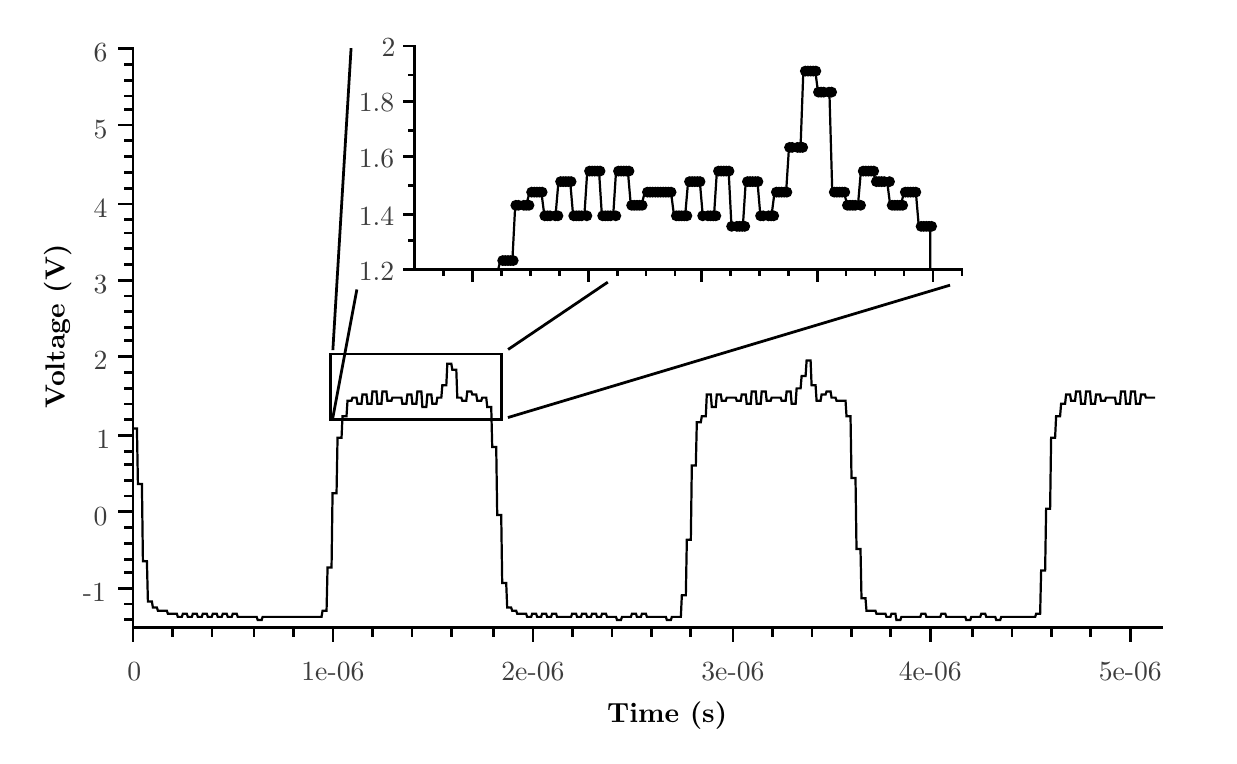
\begin{tikzpicture}{0pt}{0pt}{449pt}{269pt}
	\clip(0pt,269pt) -- (426.964pt,269pt) -- (426.964pt,13.2022pt) -- (0pt,13.2022pt) -- (0pt,269pt);
\begin{scope}
	\clip(139.785pt,262.344pt) -- (337.577pt,262.344pt) -- (337.577pt,181.515pt) -- (139.785pt,181.515pt) -- (139.785pt,262.344pt);
	\color[gray]{0}
	\draw[line width=0.8pt, line join=miter, line cap=rect](169.975pt,181.515pt) -- (171.016pt,185.557pt) -- (172.057pt,185.557pt) -- (173.098pt,185.557pt) -- (174.139pt,185.557pt) -- (175.18pt,185.557pt) -- (176.221pt,205.764pt) -- (177.262pt,205.764pt) -- (178.303pt,205.764pt) -- (179.344pt,205.764pt) -- (180.385pt,205.764pt) -- (181.426pt,209.805pt) -- (182.467pt,209.805pt) -- (183.508pt,209.805pt) -- (184.549pt,209.805pt) -- (185.59pt,209.805pt) -- (186.631pt,201.722pt) -- (187.672pt,201.722pt) -- (188.713pt,201.722pt) -- (189.754pt,201.722pt) -- (190.795pt,201.722pt) -- (191.836pt,213.847pt) -- (192.877pt,213.847pt) -- (193.918pt,213.847pt) -- (194.959pt,213.847pt) -- (196pt,213.847pt) -- (197.041pt,201.722pt) -- (198.082pt,201.722pt) -- (199.123pt,201.722pt) -- (200.164pt,201.722pt) -- (201.205pt,201.722pt) -- (202.246pt,217.888pt) -- (203.287pt,217.888pt) -- (204.328pt,217.888pt) -- (205.369pt,217.888pt) -- (206.41pt,217.888pt) -- (207.451pt,201.722pt) -- (208.492pt,201.722pt) -- (209.533pt,201.722pt) -- (210.574pt,201.722pt) -- (211.615pt,201.722pt) -- (212.656pt,217.888pt) -- (213.697pt,217.888pt) -- (214.738pt,217.888pt) -- (215.779pt,217.888pt) -- (216.82pt,217.888pt) -- (217.861pt,205.764pt) -- (218.902pt,205.764pt) -- (219.943pt,205.764pt) -- (220.984pt,205.764pt) -- (222.025pt,205.764pt) -- (223.066pt,209.805pt) -- (224.107pt,209.805pt) -- (225.148pt,209.805pt) -- (226.189pt,209.805pt) -- (227.23pt,209.805pt) -- (228.271pt,209.805pt) -- (229.312pt,209.805pt) -- (230.353pt,209.805pt) -- (231.394pt,209.805pt) -- (232.435pt,209.805pt) -- (233.476pt,201.722pt) -- (234.517pt,201.722pt) -- (235.558pt,201.722pt) -- (236.599pt,201.722pt) -- (237.64pt,201.722pt) -- (238.681pt,213.847pt) -- (239.722pt,213.847pt) -- (240.763pt,213.847pt) -- (241.804pt,213.847pt) -- (242.845pt,213.847pt) -- (243.886pt,201.722pt) -- (244.927pt,201.722pt) -- (245.968pt,201.722pt) -- (247.009pt,201.722pt) -- (248.05pt,201.722pt) -- (249.091pt,217.888pt) -- (250.132pt,217.888pt) -- (251.173pt,217.888pt) -- (252.214pt,217.888pt) -- (253.255pt,217.888pt) -- (254.296pt,197.681pt) -- (255.337pt,197.681pt) -- (256.378pt,197.681pt) -- (257.419pt,197.681pt) -- (258.46pt,197.681pt) -- (259.501pt,213.847pt) -- (260.542pt,213.847pt) -- (261.583pt,213.847pt) -- (262.624pt,213.847pt) -- (263.665pt,213.847pt) -- (264.706pt,201.722pt) -- (265.747pt,201.722pt) -- (266.788pt,201.722pt) -- (267.829pt,201.722pt) -- (268.87pt,201.722pt) -- (269.911pt,209.805pt) -- (270.952pt,209.805pt) -- (271.993pt,209.805pt) -- (273.034pt,209.805pt) -- (274.075pt,209.805pt) -- (275.116pt,225.971pt) -- (276.157pt,225.971pt) -- (277.198pt,225.971pt) -- (278.24pt,225.971pt) -- (279.281pt,225.971pt) -- (280.322pt,254.261pt) -- (281.363pt,254.261pt) -- (282.404pt,254.261pt) -- (283.445pt,254.261pt) -- (284.486pt,254.261pt) -- (285.527pt,246.178pt) -- (286.568pt,246.178pt) -- (287.609pt,246.178pt) -- (288.65pt,246.178pt) -- (289.691pt,246.178pt) -- (290.732pt,209.805pt) -- (291.773pt,209.805pt) -- (292.814pt,209.805pt) -- (293.855pt,209.805pt) -- (294.896pt,209.805pt) -- (295.937pt,205.764pt) -- (296.978pt,205.764pt) -- (298.019pt,205.764pt) -- (299.06pt,205.764pt) -- (300.101pt,205.764pt) -- (301.142pt,217.888pt) -- (302.183pt,217.888pt) -- (303.224pt,217.888pt) -- (304.265pt,217.888pt) -- (305.306pt,217.888pt) -- (306.347pt,213.847pt) -- (307.388pt,213.847pt) -- (308.429pt,213.847pt) -- (309.47pt,213.847pt) -- (310.511pt,213.847pt) -- (311.552pt,205.764pt) -- (312.593pt,205.764pt) -- (313.634pt,205.764pt) -- (314.675pt,205.764pt) -- (315.716pt,205.764pt) -- (316.757pt,209.805pt) -- (317.798pt,209.805pt) -- (318.839pt,209.805pt) -- (319.88pt,209.805pt) -- (320.921pt,209.805pt) -- (321.962pt,197.681pt) -- (323.003pt,197.681pt) -- (324.044pt,197.681pt) -- (325.085pt,197.681pt) -- (326.126pt,197.681pt) -- (326.126pt,181.515pt);
	\color[gray]{0}
	\fill(171.641pt,184.843pt) ellipse (1.42638pt and 1.42638pt);
	\draw[line width=1pt, line join=miter, line cap=rect](171.641pt,184.843pt) ellipse (1.42638pt and 1.42638pt);
	\fill(172.592pt,184.843pt) ellipse (1.42638pt and 1.42638pt);
	\draw[line width=1pt, line join=miter, line cap=rect](172.592pt,184.843pt) ellipse (1.42638pt and 1.42638pt);
	\fill(173.543pt,184.843pt) ellipse (1.42638pt and 1.42638pt);
	\draw[line width=1pt, line join=miter, line cap=rect](173.543pt,184.843pt) ellipse (1.42638pt and 1.42638pt);
	\fill(174.494pt,184.843pt) ellipse (1.42638pt and 1.42638pt);
	\draw[line width=1pt, line join=miter, line cap=rect](174.494pt,184.843pt) ellipse (1.42638pt and 1.42638pt);
	\fill(175.445pt,184.843pt) ellipse (1.42638pt and 1.42638pt);
	\draw[line width=1pt, line join=miter, line cap=rect](175.445pt,184.843pt) ellipse (1.42638pt and 1.42638pt);
	\fill(176.396pt,204.813pt) ellipse (1.42638pt and 1.42638pt);
	\draw[line width=1pt, line join=miter, line cap=rect](176.396pt,204.813pt) ellipse (1.42638pt and 1.42638pt);
	\fill(177.347pt,204.813pt) ellipse (1.42638pt and 1.42638pt);
	\draw[line width=1pt, line join=miter, line cap=rect](177.347pt,204.813pt) ellipse (1.42638pt and 1.42638pt);
	\fill(179.249pt,204.813pt) ellipse (1.42638pt and 1.42638pt);
	\draw[line width=1pt, line join=miter, line cap=rect](179.249pt,204.813pt) ellipse (1.42638pt and 1.42638pt);
	\fill(180.2pt,204.813pt) ellipse (1.42638pt and 1.42638pt);
	\draw[line width=1pt, line join=miter, line cap=rect](180.2pt,204.813pt) ellipse (1.42638pt and 1.42638pt);
	\fill(181.15pt,204.813pt) ellipse (1.42638pt and 1.42638pt);
	\draw[line width=1pt, line join=miter, line cap=rect](181.15pt,204.813pt) ellipse (1.42638pt and 1.42638pt);
	\fill(182.101pt,209.567pt) ellipse (1.42638pt and 1.42638pt);
	\draw[line width=1pt, line join=miter, line cap=rect](182.101pt,209.567pt) ellipse (1.42638pt and 1.42638pt);
	\fill(183.052pt,209.567pt) ellipse (1.42638pt and 1.42638pt);
	\draw[line width=1pt, line join=miter, line cap=rect](183.052pt,209.567pt) ellipse (1.42638pt and 1.42638pt);
	\fill(184.003pt,209.567pt) ellipse (1.42638pt and 1.42638pt);
	\draw[line width=1pt, line join=miter, line cap=rect](184.003pt,209.567pt) ellipse (1.42638pt and 1.42638pt);
	\fill(184.954pt,209.567pt) ellipse (1.42638pt and 1.42638pt);
	\draw[line width=1pt, line join=miter, line cap=rect](184.954pt,209.567pt) ellipse (1.42638pt and 1.42638pt);
	\fill(185.905pt,209.567pt) ellipse (1.42638pt and 1.42638pt);
	\draw[line width=1pt, line join=miter, line cap=rect](185.905pt,209.567pt) ellipse (1.42638pt and 1.42638pt);
	\fill(186.856pt,201.009pt) ellipse (1.42638pt and 1.42638pt);
	\draw[line width=1pt, line join=miter, line cap=rect](186.856pt,201.009pt) ellipse (1.42638pt and 1.42638pt);
	\fill(187.807pt,201.009pt) ellipse (1.42638pt and 1.42638pt);
	\draw[line width=1pt, line join=miter, line cap=rect](187.807pt,201.009pt) ellipse (1.42638pt and 1.42638pt);
	\fill(188.758pt,201.009pt) ellipse (1.42638pt and 1.42638pt);
	\draw[line width=1pt, line join=miter, line cap=rect](188.758pt,201.009pt) ellipse (1.42638pt and 1.42638pt);
	\fill(190.66pt,201.009pt) ellipse (1.42638pt and 1.42638pt);
	\draw[line width=1pt, line join=miter, line cap=rect](190.66pt,201.009pt) ellipse (1.42638pt and 1.42638pt);
	\fill(191.611pt,201.009pt) ellipse (1.42638pt and 1.42638pt);
	\draw[line width=1pt, line join=miter, line cap=rect](191.611pt,201.009pt) ellipse (1.42638pt and 1.42638pt);
	\fill(192.562pt,213.371pt) ellipse (1.42638pt and 1.42638pt);
	\draw[line width=1pt, line join=miter, line cap=rect](192.562pt,213.371pt) ellipse (1.42638pt and 1.42638pt);
	\fill(193.512pt,213.371pt) ellipse (1.42638pt and 1.42638pt);
	\draw[line width=1pt, line join=miter, line cap=rect](193.512pt,213.371pt) ellipse (1.42638pt and 1.42638pt);
	\fill(194.463pt,213.371pt) ellipse (1.42638pt and 1.42638pt);
	\draw[line width=1pt, line join=miter, line cap=rect](194.463pt,213.371pt) ellipse (1.42638pt and 1.42638pt);
	\fill(195.414pt,213.371pt) ellipse (1.42638pt and 1.42638pt);
	\draw[line width=1pt, line join=miter, line cap=rect](195.414pt,213.371pt) ellipse (1.42638pt and 1.42638pt);
	\fill(196.365pt,213.371pt) ellipse (1.42638pt and 1.42638pt);
	\draw[line width=1pt, line join=miter, line cap=rect](196.365pt,213.371pt) ellipse (1.42638pt and 1.42638pt);
	\fill(197.316pt,201.009pt) ellipse (1.42638pt and 1.42638pt);
	\draw[line width=1pt, line join=miter, line cap=rect](197.316pt,201.009pt) ellipse (1.42638pt and 1.42638pt);
	\fill(198.267pt,201.009pt) ellipse (1.42638pt and 1.42638pt);
	\draw[line width=1pt, line join=miter, line cap=rect](198.267pt,201.009pt) ellipse (1.42638pt and 1.42638pt);
	\fill(199.218pt,201.009pt) ellipse (1.42638pt and 1.42638pt);
	\draw[line width=1pt, line join=miter, line cap=rect](199.218pt,201.009pt) ellipse (1.42638pt and 1.42638pt);
	\fill(200.169pt,201.009pt) ellipse (1.42638pt and 1.42638pt);
	\draw[line width=1pt, line join=miter, line cap=rect](200.169pt,201.009pt) ellipse (1.42638pt and 1.42638pt);
	\fill(202.071pt,201.009pt) ellipse (1.42638pt and 1.42638pt);
	\draw[line width=1pt, line join=miter, line cap=rect](202.071pt,201.009pt) ellipse (1.42638pt and 1.42638pt);
	\fill(203.022pt,217.175pt) ellipse (1.42638pt and 1.42638pt);
	\draw[line width=1pt, line join=miter, line cap=rect](203.022pt,217.175pt) ellipse (1.42638pt and 1.42638pt);
	\fill(203.973pt,217.175pt) ellipse (1.42638pt and 1.42638pt);
	\draw[line width=1pt, line join=miter, line cap=rect](203.973pt,217.175pt) ellipse (1.42638pt and 1.42638pt);
	\fill(204.923pt,217.175pt) ellipse (1.42638pt and 1.42638pt);
	\draw[line width=1pt, line join=miter, line cap=rect](204.923pt,217.175pt) ellipse (1.42638pt and 1.42638pt);
	\fill(205.874pt,217.175pt) ellipse (1.42638pt and 1.42638pt);
	\draw[line width=1pt, line join=miter, line cap=rect](205.874pt,217.175pt) ellipse (1.42638pt and 1.42638pt);
	\fill(206.825pt,217.175pt) ellipse (1.42638pt and 1.42638pt);
	\draw[line width=1pt, line join=miter, line cap=rect](206.825pt,217.175pt) ellipse (1.42638pt and 1.42638pt);
	\fill(207.776pt,201.009pt) ellipse (1.42638pt and 1.42638pt);
	\draw[line width=1pt, line join=miter, line cap=rect](207.776pt,201.009pt) ellipse (1.42638pt and 1.42638pt);
	\fill(208.727pt,201.009pt) ellipse (1.42638pt and 1.42638pt);
	\draw[line width=1pt, line join=miter, line cap=rect](208.727pt,201.009pt) ellipse (1.42638pt and 1.42638pt);
	\fill(209.678pt,201.009pt) ellipse (1.42638pt and 1.42638pt);
	\draw[line width=1pt, line join=miter, line cap=rect](209.678pt,201.009pt) ellipse (1.42638pt and 1.42638pt);
	\fill(210.629pt,201.009pt) ellipse (1.42638pt and 1.42638pt);
	\draw[line width=1pt, line join=miter, line cap=rect](210.629pt,201.009pt) ellipse (1.42638pt and 1.42638pt);
	\fill(212.531pt,201.009pt) ellipse (1.42638pt and 1.42638pt);
	\draw[line width=1pt, line join=miter, line cap=rect](212.531pt,201.009pt) ellipse (1.42638pt and 1.42638pt);
	\fill(213.482pt,217.175pt) ellipse (1.42638pt and 1.42638pt);
	\draw[line width=1pt, line join=miter, line cap=rect](213.482pt,217.175pt) ellipse (1.42638pt and 1.42638pt);
	\fill(214.433pt,217.175pt) ellipse (1.42638pt and 1.42638pt);
	\draw[line width=1pt, line join=miter, line cap=rect](214.433pt,217.175pt) ellipse (1.42638pt and 1.42638pt);
	\fill(215.384pt,217.175pt) ellipse (1.42638pt and 1.42638pt);
	\draw[line width=1pt, line join=miter, line cap=rect](215.384pt,217.175pt) ellipse (1.42638pt and 1.42638pt);
	\fill(216.335pt,217.175pt) ellipse (1.42638pt and 1.42638pt);
	\draw[line width=1pt, line join=miter, line cap=rect](216.335pt,217.175pt) ellipse (1.42638pt and 1.42638pt);
	\fill(217.285pt,217.175pt) ellipse (1.42638pt and 1.42638pt);
	\draw[line width=1pt, line join=miter, line cap=rect](217.285pt,217.175pt) ellipse (1.42638pt and 1.42638pt);
	\fill(218.236pt,204.813pt) ellipse (1.42638pt and 1.42638pt);
	\draw[line width=1pt, line join=miter, line cap=rect](218.236pt,204.813pt) ellipse (1.42638pt and 1.42638pt);
	\fill(219.187pt,204.813pt) ellipse (1.42638pt and 1.42638pt);
	\draw[line width=1pt, line join=miter, line cap=rect](219.187pt,204.813pt) ellipse (1.42638pt and 1.42638pt);
	\fill(220.138pt,204.813pt) ellipse (1.42638pt and 1.42638pt);
	\draw[line width=1pt, line join=miter, line cap=rect](220.138pt,204.813pt) ellipse (1.42638pt and 1.42638pt);
	\fill(221.089pt,204.813pt) ellipse (1.42638pt and 1.42638pt);
	\draw[line width=1pt, line join=miter, line cap=rect](221.089pt,204.813pt) ellipse (1.42638pt and 1.42638pt);
	\fill(222.04pt,204.813pt) ellipse (1.42638pt and 1.42638pt);
	\draw[line width=1pt, line join=miter, line cap=rect](222.04pt,204.813pt) ellipse (1.42638pt and 1.42638pt);
	\fill(223.942pt,209.567pt) ellipse (1.42638pt and 1.42638pt);
	\draw[line width=1pt, line join=miter, line cap=rect](223.942pt,209.567pt) ellipse (1.42638pt and 1.42638pt);
	\fill(224.893pt,209.567pt) ellipse (1.42638pt and 1.42638pt);
	\draw[line width=1pt, line join=miter, line cap=rect](224.893pt,209.567pt) ellipse (1.42638pt and 1.42638pt);
	\fill(225.844pt,209.567pt) ellipse (1.42638pt and 1.42638pt);
	\draw[line width=1pt, line join=miter, line cap=rect](225.844pt,209.567pt) ellipse (1.42638pt and 1.42638pt);
	\fill(226.795pt,209.567pt) ellipse (1.42638pt and 1.42638pt);
	\draw[line width=1pt, line join=miter, line cap=rect](226.795pt,209.567pt) ellipse (1.42638pt and 1.42638pt);
	\fill(227.746pt,209.567pt) ellipse (1.42638pt and 1.42638pt);
	\draw[line width=1pt, line join=miter, line cap=rect](227.746pt,209.567pt) ellipse (1.42638pt and 1.42638pt);
	\fill(228.697pt,209.567pt) ellipse (1.42638pt and 1.42638pt);
	\draw[line width=1pt, line join=miter, line cap=rect](228.697pt,209.567pt) ellipse (1.42638pt and 1.42638pt);
	\fill(229.647pt,209.567pt) ellipse (1.42638pt and 1.42638pt);
	\draw[line width=1pt, line join=miter, line cap=rect](229.647pt,209.567pt) ellipse (1.42638pt and 1.42638pt);
	\fill(230.598pt,209.567pt) ellipse (1.42638pt and 1.42638pt);
	\draw[line width=1pt, line join=miter, line cap=rect](230.598pt,209.567pt) ellipse (1.42638pt and 1.42638pt);
	\fill(231.549pt,209.567pt) ellipse (1.42638pt and 1.42638pt);
	\draw[line width=1pt, line join=miter, line cap=rect](231.549pt,209.567pt) ellipse (1.42638pt and 1.42638pt);
	\fill(232.5pt,209.567pt) ellipse (1.42638pt and 1.42638pt);
	\draw[line width=1pt, line join=miter, line cap=rect](232.5pt,209.567pt) ellipse (1.42638pt and 1.42638pt);
	\fill(234.402pt,201.009pt) ellipse (1.42638pt and 1.42638pt);
	\draw[line width=1pt, line join=miter, line cap=rect](234.402pt,201.009pt) ellipse (1.42638pt and 1.42638pt);
	\fill(235.353pt,201.009pt) ellipse (1.42638pt and 1.42638pt);
	\draw[line width=1pt, line join=miter, line cap=rect](235.353pt,201.009pt) ellipse (1.42638pt and 1.42638pt);
	\fill(236.304pt,201.009pt) ellipse (1.42638pt and 1.42638pt);
	\draw[line width=1pt, line join=miter, line cap=rect](236.304pt,201.009pt) ellipse (1.42638pt and 1.42638pt);
	\fill(237.255pt,201.009pt) ellipse (1.42638pt and 1.42638pt);
	\draw[line width=1pt, line join=miter, line cap=rect](237.255pt,201.009pt) ellipse (1.42638pt and 1.42638pt);
	\fill(238.206pt,201.009pt) ellipse (1.42638pt and 1.42638pt);
	\draw[line width=1pt, line join=miter, line cap=rect](238.206pt,201.009pt) ellipse (1.42638pt and 1.42638pt);
	\fill(239.157pt,213.371pt) ellipse (1.42638pt and 1.42638pt);
	\draw[line width=1pt, line join=miter, line cap=rect](239.157pt,213.371pt) ellipse (1.42638pt and 1.42638pt);
	\fill(240.108pt,213.371pt) ellipse (1.42638pt and 1.42638pt);
	\draw[line width=1pt, line join=miter, line cap=rect](240.108pt,213.371pt) ellipse (1.42638pt and 1.42638pt);
	\fill(241.058pt,213.371pt) ellipse (1.42638pt and 1.42638pt);
	\draw[line width=1pt, line join=miter, line cap=rect](241.058pt,213.371pt) ellipse (1.42638pt and 1.42638pt);
	\fill(242.009pt,213.371pt) ellipse (1.42638pt and 1.42638pt);
	\draw[line width=1pt, line join=miter, line cap=rect](242.009pt,213.371pt) ellipse (1.42638pt and 1.42638pt);
	\fill(242.96pt,213.371pt) ellipse (1.42638pt and 1.42638pt);
	\draw[line width=1pt, line join=miter, line cap=rect](242.96pt,213.371pt) ellipse (1.42638pt and 1.42638pt);
	\fill(243.911pt,201.009pt) ellipse (1.42638pt and 1.42638pt);
	\draw[line width=1pt, line join=miter, line cap=rect](243.911pt,201.009pt) ellipse (1.42638pt and 1.42638pt);
	\fill(245.813pt,201.009pt) ellipse (1.42638pt and 1.42638pt);
	\draw[line width=1pt, line join=miter, line cap=rect](245.813pt,201.009pt) ellipse (1.42638pt and 1.42638pt);
	\fill(246.764pt,201.009pt) ellipse (1.42638pt and 1.42638pt);
	\draw[line width=1pt, line join=miter, line cap=rect](246.764pt,201.009pt) ellipse (1.42638pt and 1.42638pt);
	\fill(247.715pt,201.009pt) ellipse (1.42638pt and 1.42638pt);
	\draw[line width=1pt, line join=miter, line cap=rect](247.715pt,201.009pt) ellipse (1.42638pt and 1.42638pt);
	\fill(248.666pt,201.009pt) ellipse (1.42638pt and 1.42638pt);
	\draw[line width=1pt, line join=miter, line cap=rect](248.666pt,201.009pt) ellipse (1.42638pt and 1.42638pt);
	\fill(249.617pt,217.175pt) ellipse (1.42638pt and 1.42638pt);
	\draw[line width=1pt, line join=miter, line cap=rect](249.617pt,217.175pt) ellipse (1.42638pt and 1.42638pt);
	\fill(250.568pt,217.175pt) ellipse (1.42638pt and 1.42638pt);
	\draw[line width=1pt, line join=miter, line cap=rect](250.568pt,217.175pt) ellipse (1.42638pt and 1.42638pt);
	\fill(251.519pt,217.175pt) ellipse (1.42638pt and 1.42638pt);
	\draw[line width=1pt, line join=miter, line cap=rect](251.519pt,217.175pt) ellipse (1.42638pt and 1.42638pt);
	\fill(252.47pt,217.175pt) ellipse (1.42638pt and 1.42638pt);
	\draw[line width=1pt, line join=miter, line cap=rect](252.47pt,217.175pt) ellipse (1.42638pt and 1.42638pt);
	\fill(253.42pt,217.175pt) ellipse (1.42638pt and 1.42638pt);
	\draw[line width=1pt, line join=miter, line cap=rect](253.42pt,217.175pt) ellipse (1.42638pt and 1.42638pt);
	\fill(254.371pt,197.205pt) ellipse (1.42638pt and 1.42638pt);
	\draw[line width=1pt, line join=miter, line cap=rect](254.371pt,197.205pt) ellipse (1.42638pt and 1.42638pt);
	\fill(256.273pt,197.205pt) ellipse (1.42638pt and 1.42638pt);
	\draw[line width=1pt, line join=miter, line cap=rect](256.273pt,197.205pt) ellipse (1.42638pt and 1.42638pt);
	\fill(257.224pt,197.205pt) ellipse (1.42638pt and 1.42638pt);
	\draw[line width=1pt, line join=miter, line cap=rect](257.224pt,197.205pt) ellipse (1.42638pt and 1.42638pt);
	\fill(258.175pt,197.205pt) ellipse (1.42638pt and 1.42638pt);
	\draw[line width=1pt, line join=miter, line cap=rect](258.175pt,197.205pt) ellipse (1.42638pt and 1.42638pt);
	\fill(259.126pt,197.205pt) ellipse (1.42638pt and 1.42638pt);
	\draw[line width=1pt, line join=miter, line cap=rect](259.126pt,197.205pt) ellipse (1.42638pt and 1.42638pt);
	\fill(260.077pt,213.371pt) ellipse (1.42638pt and 1.42638pt);
	\draw[line width=1pt, line join=miter, line cap=rect](260.077pt,213.371pt) ellipse (1.42638pt and 1.42638pt);
	\fill(261.028pt,213.371pt) ellipse (1.42638pt and 1.42638pt);
	\draw[line width=1pt, line join=miter, line cap=rect](261.028pt,213.371pt) ellipse (1.42638pt and 1.42638pt);
	\fill(261.979pt,213.371pt) ellipse (1.42638pt and 1.42638pt);
	\draw[line width=1pt, line join=miter, line cap=rect](261.979pt,213.371pt) ellipse (1.42638pt and 1.42638pt);
	\fill(262.93pt,213.371pt) ellipse (1.42638pt and 1.42638pt);
	\draw[line width=1pt, line join=miter, line cap=rect](262.93pt,213.371pt) ellipse (1.42638pt and 1.42638pt);
	\fill(263.881pt,213.371pt) ellipse (1.42638pt and 1.42638pt);
	\draw[line width=1pt, line join=miter, line cap=rect](263.881pt,213.371pt) ellipse (1.42638pt and 1.42638pt);
	\fill(264.832pt,201.009pt) ellipse (1.42638pt and 1.42638pt);
	\draw[line width=1pt, line join=miter, line cap=rect](264.832pt,201.009pt) ellipse (1.42638pt and 1.42638pt);
	\fill(265.782pt,201.009pt) ellipse (1.42638pt and 1.42638pt);
	\draw[line width=1pt, line join=miter, line cap=rect](265.782pt,201.009pt) ellipse (1.42638pt and 1.42638pt);
	\fill(267.684pt,201.009pt) ellipse (1.42638pt and 1.42638pt);
	\draw[line width=1pt, line join=miter, line cap=rect](267.684pt,201.009pt) ellipse (1.42638pt and 1.42638pt);
	\fill(268.635pt,201.009pt) ellipse (1.42638pt and 1.42638pt);
	\draw[line width=1pt, line join=miter, line cap=rect](268.635pt,201.009pt) ellipse (1.42638pt and 1.42638pt);
	\fill(269.586pt,201.009pt) ellipse (1.42638pt and 1.42638pt);
	\draw[line width=1pt, line join=miter, line cap=rect](269.586pt,201.009pt) ellipse (1.42638pt and 1.42638pt);
	\fill(270.537pt,209.567pt) ellipse (1.42638pt and 1.42638pt);
	\draw[line width=1pt, line join=miter, line cap=rect](270.537pt,209.567pt) ellipse (1.42638pt and 1.42638pt);
	\fill(271.488pt,209.567pt) ellipse (1.42638pt and 1.42638pt);
	\draw[line width=1pt, line join=miter, line cap=rect](271.488pt,209.567pt) ellipse (1.42638pt and 1.42638pt);
	\fill(272.439pt,209.567pt) ellipse (1.42638pt and 1.42638pt);
	\draw[line width=1pt, line join=miter, line cap=rect](272.439pt,209.567pt) ellipse (1.42638pt and 1.42638pt);
	\fill(273.39pt,209.567pt) ellipse (1.42638pt and 1.42638pt);
	\draw[line width=1pt, line join=miter, line cap=rect](273.39pt,209.567pt) ellipse (1.42638pt and 1.42638pt);
	\fill(274.341pt,209.567pt) ellipse (1.42638pt and 1.42638pt);
	\draw[line width=1pt, line join=miter, line cap=rect](274.341pt,209.567pt) ellipse (1.42638pt and 1.42638pt);
	\fill(275.292pt,225.733pt) ellipse (1.42638pt and 1.42638pt);
	\draw[line width=1pt, line join=miter, line cap=rect](275.292pt,225.733pt) ellipse (1.42638pt and 1.42638pt);
	\fill(276.243pt,225.733pt) ellipse (1.42638pt and 1.42638pt);
	\draw[line width=1pt, line join=miter, line cap=rect](276.243pt,225.733pt) ellipse (1.42638pt and 1.42638pt);
	\fill(278.144pt,225.733pt) ellipse (1.42638pt and 1.42638pt);
	\draw[line width=1pt, line join=miter, line cap=rect](278.144pt,225.733pt) ellipse (1.42638pt and 1.42638pt);
	\fill(279.095pt,225.733pt) ellipse (1.42638pt and 1.42638pt);
	\draw[line width=1pt, line join=miter, line cap=rect](279.095pt,225.733pt) ellipse (1.42638pt and 1.42638pt);
	\fill(280.046pt,225.733pt) ellipse (1.42638pt and 1.42638pt);
	\draw[line width=1pt, line join=miter, line cap=rect](280.046pt,225.733pt) ellipse (1.42638pt and 1.42638pt);
	\fill(280.997pt,253.31pt) ellipse (1.42638pt and 1.42638pt);
	\draw[line width=1pt, line join=miter, line cap=rect](280.997pt,253.31pt) ellipse (1.42638pt and 1.42638pt);
	\fill(281.948pt,253.31pt) ellipse (1.42638pt and 1.42638pt);
	\draw[line width=1pt, line join=miter, line cap=rect](281.948pt,253.31pt) ellipse (1.42638pt and 1.42638pt);
	\fill(282.899pt,253.31pt) ellipse (1.42638pt and 1.42638pt);
	\draw[line width=1pt, line join=miter, line cap=rect](282.899pt,253.31pt) ellipse (1.42638pt and 1.42638pt);
	\fill(283.85pt,253.31pt) ellipse (1.42638pt and 1.42638pt);
	\draw[line width=1pt, line join=miter, line cap=rect](283.85pt,253.31pt) ellipse (1.42638pt and 1.42638pt);
	\fill(284.801pt,253.31pt) ellipse (1.42638pt and 1.42638pt);
	\draw[line width=1pt, line join=miter, line cap=rect](284.801pt,253.31pt) ellipse (1.42638pt and 1.42638pt);
	\fill(285.752pt,245.702pt) ellipse (1.42638pt and 1.42638pt);
	\draw[line width=1pt, line join=miter, line cap=rect](285.752pt,245.702pt) ellipse (1.42638pt and 1.42638pt);
	\fill(286.703pt,245.702pt) ellipse (1.42638pt and 1.42638pt);
	\draw[line width=1pt, line join=miter, line cap=rect](286.703pt,245.702pt) ellipse (1.42638pt and 1.42638pt);
	\fill(287.654pt,245.702pt) ellipse (1.42638pt and 1.42638pt);
	\draw[line width=1pt, line join=miter, line cap=rect](287.654pt,245.702pt) ellipse (1.42638pt and 1.42638pt);
	\fill(289.555pt,245.702pt) ellipse (1.42638pt and 1.42638pt);
	\draw[line width=1pt, line join=miter, line cap=rect](289.555pt,245.702pt) ellipse (1.42638pt and 1.42638pt);
	\fill(290.506pt,245.702pt) ellipse (1.42638pt and 1.42638pt);
	\draw[line width=1pt, line join=miter, line cap=rect](290.506pt,245.702pt) ellipse (1.42638pt and 1.42638pt);
	\fill(291.457pt,209.567pt) ellipse (1.42638pt and 1.42638pt);
	\draw[line width=1pt, line join=miter, line cap=rect](291.457pt,209.567pt) ellipse (1.42638pt and 1.42638pt);
	\fill(292.408pt,209.567pt) ellipse (1.42638pt and 1.42638pt);
	\draw[line width=1pt, line join=miter, line cap=rect](292.408pt,209.567pt) ellipse (1.42638pt and 1.42638pt);
	\fill(293.359pt,209.567pt) ellipse (1.42638pt and 1.42638pt);
	\draw[line width=1pt, line join=miter, line cap=rect](293.359pt,209.567pt) ellipse (1.42638pt and 1.42638pt);
	\fill(294.31pt,209.567pt) ellipse (1.42638pt and 1.42638pt);
	\draw[line width=1pt, line join=miter, line cap=rect](294.31pt,209.567pt) ellipse (1.42638pt and 1.42638pt);
	\fill(295.261pt,209.567pt) ellipse (1.42638pt and 1.42638pt);
	\draw[line width=1pt, line join=miter, line cap=rect](295.261pt,209.567pt) ellipse (1.42638pt and 1.42638pt);
	\fill(296.212pt,204.813pt) ellipse (1.42638pt and 1.42638pt);
	\draw[line width=1pt, line join=miter, line cap=rect](296.212pt,204.813pt) ellipse (1.42638pt and 1.42638pt);
	\fill(297.163pt,204.813pt) ellipse (1.42638pt and 1.42638pt);
	\draw[line width=1pt, line join=miter, line cap=rect](297.163pt,204.813pt) ellipse (1.42638pt and 1.42638pt);
	\fill(298.114pt,204.813pt) ellipse (1.42638pt and 1.42638pt);
	\draw[line width=1pt, line join=miter, line cap=rect](298.114pt,204.813pt) ellipse (1.42638pt and 1.42638pt);
	\fill(299.065pt,204.813pt) ellipse (1.42638pt and 1.42638pt);
	\draw[line width=1pt, line join=miter, line cap=rect](299.065pt,204.813pt) ellipse (1.42638pt and 1.42638pt);
	\fill(300.967pt,204.813pt) ellipse (1.42638pt and 1.42638pt);
	\draw[line width=1pt, line join=miter, line cap=rect](300.967pt,204.813pt) ellipse (1.42638pt and 1.42638pt);
	\fill(301.917pt,217.175pt) ellipse (1.42638pt and 1.42638pt);
	\draw[line width=1pt, line join=miter, line cap=rect](301.917pt,217.175pt) ellipse (1.42638pt and 1.42638pt);
	\fill(302.868pt,217.175pt) ellipse (1.42638pt and 1.42638pt);
	\draw[line width=1pt, line join=miter, line cap=rect](302.868pt,217.175pt) ellipse (1.42638pt and 1.42638pt);
	\fill(303.819pt,217.175pt) ellipse (1.42638pt and 1.42638pt);
	\draw[line width=1pt, line join=miter, line cap=rect](303.819pt,217.175pt) ellipse (1.42638pt and 1.42638pt);
	\fill(304.77pt,217.175pt) ellipse (1.42638pt and 1.42638pt);
	\draw[line width=1pt, line join=miter, line cap=rect](304.77pt,217.175pt) ellipse (1.42638pt and 1.42638pt);
	\fill(305.721pt,217.175pt) ellipse (1.42638pt and 1.42638pt);
	\draw[line width=1pt, line join=miter, line cap=rect](305.721pt,217.175pt) ellipse (1.42638pt and 1.42638pt);
	\fill(306.672pt,213.371pt) ellipse (1.42638pt and 1.42638pt);
	\draw[line width=1pt, line join=miter, line cap=rect](306.672pt,213.371pt) ellipse (1.42638pt and 1.42638pt);
	\fill(307.623pt,213.371pt) ellipse (1.42638pt and 1.42638pt);
	\draw[line width=1pt, line join=miter, line cap=rect](307.623pt,213.371pt) ellipse (1.42638pt and 1.42638pt);
	\fill(308.574pt,213.371pt) ellipse (1.42638pt and 1.42638pt);
	\draw[line width=1pt, line join=miter, line cap=rect](308.574pt,213.371pt) ellipse (1.42638pt and 1.42638pt);
	\fill(309.525pt,213.371pt) ellipse (1.42638pt and 1.42638pt);
	\draw[line width=1pt, line join=miter, line cap=rect](309.525pt,213.371pt) ellipse (1.42638pt and 1.42638pt);
	\fill(311.427pt,213.371pt) ellipse (1.42638pt and 1.42638pt);
	\draw[line width=1pt, line join=miter, line cap=rect](311.427pt,213.371pt) ellipse (1.42638pt and 1.42638pt);
	\fill(312.378pt,204.813pt) ellipse (1.42638pt and 1.42638pt);
	\draw[line width=1pt, line join=miter, line cap=rect](312.378pt,204.813pt) ellipse (1.42638pt and 1.42638pt);
	\fill(313.328pt,204.813pt) ellipse (1.42638pt and 1.42638pt);
	\draw[line width=1pt, line join=miter, line cap=rect](313.328pt,204.813pt) ellipse (1.42638pt and 1.42638pt);
	\fill(314.279pt,204.813pt) ellipse (1.42638pt and 1.42638pt);
	\draw[line width=1pt, line join=miter, line cap=rect](314.279pt,204.813pt) ellipse (1.42638pt and 1.42638pt);
	\fill(315.23pt,204.813pt) ellipse (1.42638pt and 1.42638pt);
	\draw[line width=1pt, line join=miter, line cap=rect](315.23pt,204.813pt) ellipse (1.42638pt and 1.42638pt);
	\fill(316.181pt,204.813pt) ellipse (1.42638pt and 1.42638pt);
	\draw[line width=1pt, line join=miter, line cap=rect](316.181pt,204.813pt) ellipse (1.42638pt and 1.42638pt);
	\fill(317.132pt,209.567pt) ellipse (1.42638pt and 1.42638pt);
	\draw[line width=1pt, line join=miter, line cap=rect](317.132pt,209.567pt) ellipse (1.42638pt and 1.42638pt);
	\fill(318.083pt,209.567pt) ellipse (1.42638pt and 1.42638pt);
	\draw[line width=1pt, line join=miter, line cap=rect](318.083pt,209.567pt) ellipse (1.42638pt and 1.42638pt);
	\fill(319.034pt,209.567pt) ellipse (1.42638pt and 1.42638pt);
	\draw[line width=1pt, line join=miter, line cap=rect](319.034pt,209.567pt) ellipse (1.42638pt and 1.42638pt);
	\fill(319.985pt,209.567pt) ellipse (1.42638pt and 1.42638pt);
	\draw[line width=1pt, line join=miter, line cap=rect](319.985pt,209.567pt) ellipse (1.42638pt and 1.42638pt);
	\fill(320.936pt,209.567pt) ellipse (1.42638pt and 1.42638pt);
	\draw[line width=1pt, line join=miter, line cap=rect](320.936pt,209.567pt) ellipse (1.42638pt and 1.42638pt);
	\fill(322.838pt,197.205pt) ellipse (1.42638pt and 1.42638pt);
	\draw[line width=1pt, line join=miter, line cap=rect](322.838pt,197.205pt) ellipse (1.42638pt and 1.42638pt);
	\fill(323.789pt,197.205pt) ellipse (1.42638pt and 1.42638pt);
	\draw[line width=1pt, line join=miter, line cap=rect](323.789pt,197.205pt) ellipse (1.42638pt and 1.42638pt);
	\fill(324.74pt,197.205pt) ellipse (1.42638pt and 1.42638pt);
	\draw[line width=1pt, line join=miter, line cap=rect](324.74pt,197.205pt) ellipse (1.42638pt and 1.42638pt);
	\fill(325.69pt,197.205pt) ellipse (1.42638pt and 1.42638pt);
	\draw[line width=1pt, line join=miter, line cap=rect](325.69pt,197.205pt) ellipse (1.42638pt and 1.42638pt);
	\fill(326.641pt,197.205pt) ellipse (1.42638pt and 1.42638pt);
	\draw[line width=1pt, line join=miter, line cap=rect](326.641pt,197.205pt) ellipse (1.42638pt and 1.42638pt);
\end{scope}
\begin{scope}
	\color[gray]{0.235294}
	\pgftext[center, base, at={\pgfpoint{126.049pt}{177.712pt}}]{1.2}
	\pgftext[center, base, at={\pgfpoint{126.049pt}{197.681pt}}]{1.4}
	\pgftext[center, base, at={\pgfpoint{126.049pt}{218.601pt}}]{1.6}
	\pgftext[center, base, at={\pgfpoint{126.049pt}{238.571pt}}]{1.8}
	\pgftext[center, base, at={\pgfpoint{130.373pt}{258.54pt}}]{2}
	\color[gray]{0}
	\draw[line width=1pt, line join=bevel, line cap=rect](139.785pt,191.975pt) -- (137.884pt,191.975pt);
	\draw[line width=1pt, line join=bevel, line cap=rect](139.785pt,211.945pt) -- (137.884pt,211.945pt);
	\draw[line width=1pt, line join=bevel, line cap=rect](139.785pt,231.914pt) -- (137.884pt,231.914pt);
	\draw[line width=1pt, line join=bevel, line cap=rect](139.785pt,251.883pt) -- (137.884pt,251.883pt);
	\draw[line width=1pt, line join=bevel, line cap=rect](139.785pt,181.515pt) -- (135.982pt,181.515pt);
	\draw[line width=1pt, line join=bevel, line cap=rect](139.785pt,201.485pt) -- (135.982pt,201.485pt);
	\draw[line width=1pt, line join=bevel, line cap=rect](139.785pt,222.405pt) -- (135.982pt,222.405pt);
	\draw[line width=1pt, line join=bevel, line cap=rect](139.785pt,242.374pt) -- (135.982pt,242.374pt);
	\draw[line width=1pt, line join=bevel, line cap=rect](139.785pt,262.344pt) -- (135.982pt,262.344pt);
	\draw[line width=1pt, line join=bevel, line cap=rect](139.785pt,262.344pt) -- (139.785pt,181.515pt);
	\draw[line width=1pt, line join=bevel, line cap=rect](150.246pt,181.515pt) -- (150.246pt,179.613pt);
	\draw[line width=1pt, line join=bevel, line cap=rect](171.166pt,181.515pt) -- (171.166pt,179.613pt);
	\draw[line width=1pt, line join=bevel, line cap=rect](192.086pt,181.515pt) -- (192.086pt,179.613pt);
	\draw[line width=1pt, line join=bevel, line cap=rect](213.006pt,181.515pt) -- (213.006pt,179.613pt);
	\draw[line width=1pt, line join=bevel, line cap=rect](233.927pt,181.515pt) -- (233.927pt,179.613pt);
	\draw[line width=1pt, line join=bevel, line cap=rect](253.896pt,181.515pt) -- (253.896pt,179.613pt);
	\draw[line width=1pt, line join=bevel, line cap=rect](274.816pt,181.515pt) -- (274.816pt,179.613pt);
	\draw[line width=1pt, line join=bevel, line cap=rect](295.736pt,181.515pt) -- (295.736pt,179.613pt);
	\draw[line width=1pt, line join=bevel, line cap=rect](316.657pt,181.515pt) -- (316.657pt,179.613pt);
	\draw[line width=1pt, line join=bevel, line cap=rect](337.577pt,181.515pt) -- (337.577pt,179.613pt);
	\draw[line width=1pt, line join=bevel, line cap=rect](181.626pt,181.515pt) -- (181.626pt,179.613pt);
	\draw[line width=1pt, line join=bevel, line cap=rect](223.466pt,181.515pt) -- (223.466pt,179.613pt);
	\draw[line width=1pt, line join=bevel, line cap=rect](264.356pt,181.515pt) -- (264.356pt,179.613pt);
	\draw[line width=1pt, line join=bevel, line cap=rect](306.197pt,181.515pt) -- (306.197pt,179.613pt);
	\draw[line width=1pt, line join=bevel, line cap=rect](160.706pt,181.515pt) -- (160.706pt,177.712pt);
	\draw[line width=1pt, line join=bevel, line cap=rect](202.546pt,181.515pt) -- (202.546pt,177.712pt);
	\draw[line width=1pt, line join=bevel, line cap=rect](243.436pt,181.515pt) -- (243.436pt,177.712pt);
	\draw[line width=1pt, line join=bevel, line cap=rect](285.276pt,181.515pt) -- (285.276pt,177.712pt);
	\draw[line width=1pt, line join=bevel, line cap=rect](327.117pt,181.515pt) -- (327.117pt,177.712pt);
	\draw[line width=1pt, line join=bevel, line cap=rect](139.785pt,181.515pt) -- (337.577pt,181.515pt);
\end{scope}
\begin{scope}
	\clip(38.0368pt,261.393pt) -- (409.847pt,261.393pt) -- (409.847pt,52.19pt) -- (38.0368pt,52.19pt) -- (38.0368pt,261.393pt);
	\color[gray]{0}
	\draw[line width=0.8pt, line join=miter, line cap=rect](38.3975pt,124.156pt) -- (38.7581pt,124.156pt) -- (39.1187pt,124.156pt) -- (39.4794pt,124.156pt) -- (39.84pt,104.072pt) -- (40.2006pt,104.072pt) -- (40.5613pt,104.072pt) -- (40.9219pt,104.072pt) -- (41.2825pt,104.072pt) -- (41.6431pt,76.1786pt) -- (42.0038pt,76.1786pt) -- (42.3644pt,76.1786pt) -- (42.725pt,76.1786pt) -- (43.0857pt,76.1786pt) -- (43.4463pt,61.6739pt) -- (43.8069pt,61.6739pt) -- (44.1676pt,61.6739pt) -- (44.5282pt,61.6739pt) -- (44.8888pt,61.6739pt) -- (45.2495pt,59.4424pt) -- (45.6101pt,59.4424pt) -- (45.9707pt,59.4424pt) -- (46.3313pt,59.4424pt) -- (46.692pt,59.4424pt) -- (47.0526pt,58.3266pt) -- (47.4132pt,58.3266pt) -- (47.7739pt,58.3266pt) -- (48.1345pt,58.3266pt) -- (48.4951pt,58.3266pt) -- (48.8558pt,58.3266pt) -- (49.2164pt,58.3266pt) -- (49.577pt,58.3266pt) -- (49.9377pt,58.3266pt) -- (50.2983pt,58.3266pt) -- (50.6589pt,57.2109pt) -- (51.0195pt,57.2109pt) -- (51.3802pt,57.2109pt) -- (51.7408pt,57.2109pt) -- (52.1014pt,57.2109pt) -- (52.4621pt,57.2109pt) -- (52.8227pt,57.2109pt) -- (53.1833pt,57.2109pt) -- (53.544pt,57.2109pt) -- (53.9046pt,57.2109pt) -- (54.2652pt,56.0951pt) -- (54.6258pt,56.0951pt) -- (54.9865pt,56.0951pt) -- (55.3471pt,56.0951pt) -- (55.7077pt,56.0951pt) -- (56.0684pt,57.2109pt) -- (56.429pt,57.2109pt) -- (56.7896pt,57.2109pt) -- (57.1503pt,57.2109pt) -- (57.5109pt,57.2109pt) -- (57.8715pt,56.0951pt) -- (58.2322pt,56.0951pt) -- (58.5928pt,56.0951pt) -- (58.9534pt,56.0951pt) -- (59.314pt,56.0951pt) -- (59.6747pt,57.2109pt) -- (60.0353pt,57.2109pt) -- (60.3959pt,57.2109pt) -- (60.7566pt,57.2109pt) -- (61.1172pt,57.2109pt) -- (61.4778pt,56.0951pt) -- (61.8385pt,56.0951pt) -- (62.1991pt,56.0951pt) -- (62.5597pt,56.0951pt) -- (62.9204pt,56.0951pt) -- (63.281pt,57.2109pt) -- (63.6416pt,57.2109pt) -- (64.0022pt,57.2109pt) -- (64.3629pt,57.2109pt) -- (64.7235pt,57.2109pt) -- (65.0841pt,56.0951pt) -- (65.4448pt,56.0951pt) -- (65.8054pt,56.0951pt) -- (66.166pt,56.0951pt) -- (66.5267pt,56.0951pt) -- (66.8873pt,57.2109pt) -- (67.2479pt,57.2109pt) -- (67.6085pt,57.2109pt) -- (67.9692pt,57.2109pt) -- (68.3298pt,57.2109pt) -- (68.6904pt,56.0951pt) -- (69.0511pt,56.0951pt) -- (69.4117pt,56.0951pt) -- (69.7723pt,56.0951pt) -- (70.133pt,56.0951pt) -- (70.4936pt,57.2109pt) -- (70.8542pt,57.2109pt) -- (71.2149pt,57.2109pt) -- (71.5755pt,57.2109pt) -- (71.9361pt,57.2109pt) -- (72.2967pt,56.0951pt) -- (72.6574pt,56.0951pt) -- (73.018pt,56.0951pt) -- (73.3786pt,56.0951pt) -- (73.7393pt,56.0951pt) -- (74.0999pt,57.2109pt) -- (74.4605pt,57.2109pt) -- (74.8212pt,57.2109pt) -- (75.1818pt,57.2109pt) -- (75.5424pt,57.2109pt) -- (75.9031pt,56.0951pt) -- (76.2637pt,56.0951pt) -- (76.6243pt,56.0951pt) -- (76.9849pt,56.0951pt) -- (77.3456pt,56.0951pt) -- (77.7062pt,56.0951pt) -- (78.0668pt,56.0951pt) -- (78.4275pt,56.0951pt) -- (78.7881pt,56.0951pt) -- (79.1487pt,56.0951pt) -- (79.5094pt,56.0951pt) -- (79.87pt,56.0951pt) -- (80.2306pt,56.0951pt) -- (80.5913pt,56.0951pt) -- (80.9519pt,56.0951pt) -- (81.3125pt,56.0951pt) -- (81.6731pt,56.0951pt) -- (82.0338pt,56.0951pt) -- (82.3944pt,56.0951pt) -- (82.755pt,56.0951pt) -- (83.1157pt,54.9794pt) -- (83.4763pt,54.9794pt) -- (83.8369pt,54.9794pt) -- (84.1976pt,54.9794pt) -- (84.5582pt,54.9794pt) -- (84.9188pt,56.0951pt) -- (85.2794pt,56.0951pt) -- (85.6401pt,56.0951pt) -- (86.0007pt,56.0951pt) -- (86.3613pt,56.0951pt) -- (86.722pt,56.0951pt) -- (87.0826pt,56.0951pt) -- (87.4432pt,56.0951pt) -- (87.8039pt,56.0951pt) -- (88.1645pt,56.0951pt) -- (88.5251pt,56.0951pt) -- (88.8858pt,56.0951pt) -- (89.2464pt,56.0951pt) -- (89.607pt,56.0951pt) -- (89.9676pt,56.0951pt) -- (90.3283pt,56.0951pt) -- (90.6889pt,56.0951pt) -- (91.0495pt,56.0951pt) -- (91.4102pt,56.0951pt) -- (91.7708pt,56.0951pt) -- (92.1314pt,56.0951pt) -- (92.4921pt,56.0951pt) -- (92.8527pt,56.0951pt) -- (93.2133pt,56.0951pt) -- (93.574pt,56.0951pt) -- (93.9346pt,56.0951pt) -- (94.2952pt,56.0951pt) -- (94.6558pt,56.0951pt) -- (95.0165pt,56.0951pt) -- (95.3771pt,56.0951pt) -- (95.7377pt,56.0951pt) -- (96.0984pt,56.0951pt) -- (96.459pt,56.0951pt) -- (96.8196pt,56.0951pt) -- (97.1803pt,56.0951pt) -- (97.5409pt,56.0951pt) -- (97.9015pt,56.0951pt) -- (98.2621pt,56.0951pt) -- (98.6228pt,56.0951pt) -- (98.9834pt,56.0951pt) -- (99.344pt,56.0951pt) -- (99.7047pt,56.0951pt) -- (100.065pt,56.0951pt) -- (100.426pt,56.0951pt) -- (100.787pt,56.0951pt) -- (101.147pt,56.0951pt) -- (101.508pt,56.0951pt) -- (101.868pt,56.0951pt) -- (102.229pt,56.0951pt) -- (102.59pt,56.0951pt) -- (102.95pt,56.0951pt) -- (103.311pt,56.0951pt) -- (103.672pt,56.0951pt) -- (104.032pt,56.0951pt) -- (104.393pt,56.0951pt) -- (104.754pt,56.0951pt) -- (105.114pt,56.0951pt) -- (105.475pt,56.0951pt) -- (105.835pt,56.0951pt) -- (106.196pt,56.0951pt) -- (106.557pt,58.3266pt) -- (106.917pt,58.3266pt) -- (107.278pt,58.3266pt) -- (107.639pt,58.3266pt) -- (107.999pt,58.3266pt) -- (108.36pt,73.9471pt) -- (108.72pt,73.9471pt) -- (109.081pt,73.9471pt) -- (109.442pt,73.9471pt) -- (109.802pt,73.9471pt) -- (110.163pt,100.725pt) -- (110.524pt,100.725pt) -- (110.884pt,100.725pt) -- (111.245pt,100.725pt) -- (111.605pt,100.725pt) -- (111.966pt,120.808pt) -- (112.327pt,120.808pt) -- (112.687pt,120.808pt) -- (113.048pt,120.808pt) -- (113.409pt,120.808pt) -- (113.769pt,128.619pt) -- (114.13pt,128.619pt) -- (114.491pt,128.619pt) -- (114.851pt,128.619pt) -- (115.212pt,128.619pt) -- (115.572pt,134.197pt) -- (115.933pt,134.197pt) -- (116.294pt,134.197pt) -- (116.654pt,134.197pt) -- (117.015pt,134.197pt) -- (117.376pt,135.313pt) -- (117.736pt,135.313pt) -- (118.097pt,135.313pt) -- (118.457pt,135.313pt) -- (118.818pt,135.313pt) -- (119.179pt,133.082pt) -- (119.539pt,133.082pt) -- (119.9pt,133.082pt) -- (120.261pt,133.082pt) -- (120.621pt,133.082pt) -- (120.982pt,136.429pt) -- (121.343pt,136.429pt) -- (121.703pt,136.429pt) -- (122.064pt,136.429pt) -- (122.424pt,136.429pt) -- (122.785pt,133.082pt) -- (123.146pt,133.082pt) -- (123.506pt,133.082pt) -- (123.867pt,133.082pt) -- (124.228pt,133.082pt) -- (124.588pt,137.545pt) -- (124.949pt,137.545pt) -- (125.309pt,137.545pt) -- (125.67pt,137.545pt) -- (126.031pt,137.545pt) -- (126.391pt,133.082pt) -- (126.752pt,133.082pt) -- (127.113pt,133.082pt) -- (127.473pt,133.082pt) -- (127.834pt,133.082pt) -- (128.194pt,137.545pt) -- (128.555pt,137.545pt) -- (128.916pt,137.545pt) -- (129.276pt,137.545pt) -- (129.637pt,137.545pt) -- (129.998pt,134.197pt) -- (130.358pt,134.197pt) -- (130.719pt,134.197pt) -- (131.08pt,134.197pt) -- (131.44pt,134.197pt) -- (131.801pt,135.313pt) -- (132.161pt,135.313pt) -- (132.522pt,135.313pt) -- (132.883pt,135.313pt) -- (133.243pt,135.313pt) -- (133.604pt,135.313pt) -- (133.965pt,135.313pt) -- (134.325pt,135.313pt) -- (134.686pt,135.313pt) -- (135.046pt,135.313pt) -- (135.407pt,133.082pt) -- (135.768pt,133.082pt) -- (136.128pt,133.082pt) -- (136.489pt,133.082pt) -- (136.85pt,133.082pt) -- (137.21pt,136.429pt) -- (137.571pt,136.429pt) -- (137.932pt,136.429pt) -- (138.292pt,136.429pt) -- (138.653pt,136.429pt) -- (139.013pt,133.082pt) -- (139.374pt,133.082pt) -- (139.735pt,133.082pt) -- (140.095pt,133.082pt) -- (140.456pt,133.082pt) -- (140.817pt,137.545pt) -- (141.177pt,137.545pt) -- (141.538pt,137.545pt) -- (141.898pt,137.545pt) -- (142.259pt,137.545pt) -- (142.62pt,131.966pt) -- (142.98pt,131.966pt) -- (143.341pt,131.966pt) -- (143.702pt,131.966pt) -- (144.062pt,131.966pt) -- (144.423pt,136.429pt) -- (144.783pt,136.429pt) -- (145.144pt,136.429pt) -- (145.505pt,136.429pt) -- (145.865pt,136.429pt) -- (146.226pt,133.082pt) -- (146.587pt,133.082pt) -- (146.947pt,133.082pt) -- (147.308pt,133.082pt) -- (147.669pt,133.082pt) -- (148.029pt,135.313pt) -- (148.39pt,135.313pt) -- (148.75pt,135.313pt) -- (149.111pt,135.313pt) -- (149.472pt,135.313pt) -- (149.832pt,139.776pt) -- (150.193pt,139.776pt) -- (150.554pt,139.776pt) -- (150.914pt,139.776pt) -- (151.275pt,139.776pt) -- (151.635pt,147.586pt) -- (151.996pt,147.586pt) -- (152.357pt,147.586pt) -- (152.717pt,147.586pt) -- (153.078pt,147.586pt) -- (153.439pt,145.355pt) -- (153.799pt,145.355pt) -- (154.16pt,145.355pt) -- (154.521pt,145.355pt) -- (154.881pt,145.355pt) -- (155.242pt,135.313pt) -- (155.602pt,135.313pt) -- (155.963pt,135.313pt) -- (156.324pt,135.313pt) -- (156.684pt,135.313pt) -- (157.045pt,134.197pt) -- (157.406pt,134.197pt) -- (157.766pt,134.197pt) -- (158.127pt,134.197pt) -- (158.487pt,134.197pt) -- (158.848pt,137.545pt) -- (159.209pt,137.545pt) -- (159.569pt,137.545pt) -- (159.93pt,137.545pt) -- (160.291pt,137.545pt) -- (160.651pt,136.429pt) -- (161.012pt,136.429pt) -- (161.373pt,136.429pt) -- (161.733pt,136.429pt) -- (162.094pt,136.429pt) -- (162.454pt,134.197pt) -- (162.815pt,134.197pt) -- (163.176pt,134.197pt) -- (163.536pt,134.197pt) -- (163.897pt,134.197pt) -- (164.258pt,135.313pt) -- (164.618pt,135.313pt) -- (164.979pt,135.313pt) -- (165.339pt,135.313pt) -- (165.7pt,135.313pt) -- (166.061pt,131.966pt) -- (166.421pt,131.966pt) -- (166.782pt,131.966pt) -- (167.143pt,131.966pt) -- (167.503pt,131.966pt) -- (167.864pt,117.461pt) -- (168.224pt,117.461pt) -- (168.585pt,117.461pt) -- (168.946pt,117.461pt) -- (169.306pt,117.461pt) -- (169.667pt,92.9148pt) -- (170.028pt,92.9148pt) -- (170.388pt,92.9148pt) -- (170.749pt,92.9148pt) -- (171.11pt,92.9148pt) -- (171.47pt,68.3683pt) -- (171.831pt,68.3683pt) -- (172.191pt,68.3683pt) -- (172.552pt,68.3683pt) -- (172.913pt,68.3683pt) -- (173.273pt,59.4424pt) -- (173.634pt,59.4424pt) -- (173.995pt,59.4424pt) -- (174.355pt,59.4424pt) -- (174.716pt,59.4424pt) -- (175.076pt,58.3266pt) -- (175.437pt,58.3266pt) -- (175.798pt,58.3266pt) -- (176.158pt,58.3266pt) -- (176.519pt,58.3266pt) -- (176.88pt,57.2109pt) -- (177.24pt,57.2109pt) -- (177.601pt,57.2109pt) -- (177.962pt,57.2109pt) -- (178.322pt,57.2109pt) -- (178.683pt,57.2109pt) -- (179.043pt,57.2109pt) -- (179.404pt,57.2109pt) -- (179.765pt,57.2109pt) -- (180.125pt,57.2109pt) -- (180.486pt,56.0951pt) -- (180.847pt,56.0951pt) -- (181.207pt,56.0951pt) -- (181.568pt,56.0951pt) -- (181.928pt,56.0951pt) -- (182.289pt,57.2109pt) -- (182.65pt,57.2109pt) -- (183.01pt,57.2109pt) -- (183.371pt,57.2109pt) -- (183.732pt,57.2109pt) -- (184.092pt,56.0951pt) -- (184.453pt,56.0951pt) -- (184.813pt,56.0951pt) -- (185.174pt,56.0951pt) -- (185.535pt,56.0951pt) -- (185.895pt,57.2109pt) -- (186.256pt,57.2109pt) -- (186.617pt,57.2109pt) -- (186.977pt,57.2109pt) -- (187.338pt,57.2109pt) -- (187.699pt,56.0951pt) -- (188.059pt,56.0951pt) -- (188.42pt,56.0951pt) -- (188.78pt,56.0951pt) -- (189.141pt,56.0951pt) -- (189.502pt,57.2109pt) -- (189.862pt,57.2109pt) -- (190.223pt,57.2109pt) -- (190.584pt,57.2109pt) -- (190.944pt,57.2109pt) -- (191.305pt,56.0951pt) -- (191.665pt,56.0951pt) -- (192.026pt,56.0951pt) -- (192.387pt,56.0951pt) -- (192.747pt,56.0951pt) -- (193.108pt,56.0951pt) -- (193.469pt,56.0951pt) -- (193.829pt,56.0951pt) -- (194.19pt,56.0951pt) -- (194.551pt,56.0951pt) -- (194.911pt,56.0951pt) -- (195.272pt,56.0951pt) -- (195.632pt,56.0951pt) -- (195.993pt,56.0951pt) -- (196.354pt,56.0951pt) -- (196.714pt,57.2109pt) -- (197.075pt,57.2109pt) -- (197.436pt,57.2109pt) -- (197.796pt,57.2109pt) -- (198.157pt,57.2109pt) -- (198.517pt,56.0951pt) -- (198.878pt,56.0951pt) -- (199.239pt,56.0951pt) -- (199.599pt,56.0951pt) -- (199.96pt,56.0951pt) -- (200.321pt,57.2109pt) -- (200.681pt,57.2109pt) -- (201.042pt,57.2109pt) -- (201.402pt,57.2109pt) -- (201.763pt,57.2109pt) -- (202.124pt,56.0951pt) -- (202.484pt,56.0951pt) -- (202.845pt,56.0951pt) -- (203.206pt,56.0951pt) -- (203.566pt,56.0951pt) -- (203.927pt,57.2109pt) -- (204.288pt,57.2109pt) -- (204.648pt,57.2109pt) -- (205.009pt,57.2109pt) -- (205.369pt,57.2109pt) -- (205.73pt,56.0951pt) -- (206.091pt,56.0951pt) -- (206.451pt,56.0951pt) -- (206.812pt,56.0951pt) -- (207.173pt,56.0951pt) -- (207.533pt,57.2109pt) -- (207.894pt,57.2109pt) -- (208.254pt,57.2109pt) -- (208.615pt,57.2109pt) -- (208.976pt,57.2109pt) -- (209.336pt,56.0951pt) -- (209.697pt,56.0951pt) -- (210.058pt,56.0951pt) -- (210.418pt,56.0951pt) -- (210.779pt,56.0951pt) -- (211.14pt,56.0951pt) -- (211.5pt,56.0951pt) -- (211.861pt,56.0951pt) -- (212.221pt,56.0951pt) -- (212.582pt,56.0951pt) -- (212.943pt,54.9794pt) -- (213.303pt,54.9794pt) -- (213.664pt,54.9794pt) -- (214.025pt,54.9794pt) -- (214.385pt,54.9794pt) -- (214.746pt,56.0951pt) -- (215.106pt,56.0951pt) -- (215.467pt,56.0951pt) -- (215.828pt,56.0951pt) -- (216.188pt,56.0951pt) -- (216.549pt,56.0951pt) -- (216.91pt,56.0951pt) -- (217.27pt,56.0951pt) -- (217.631pt,56.0951pt) -- (217.992pt,56.0951pt) -- (218.352pt,57.2109pt) -- (218.713pt,57.2109pt) -- (219.073pt,57.2109pt) -- (219.434pt,57.2109pt) -- (219.795pt,57.2109pt) -- (220.155pt,56.0951pt) -- (220.516pt,56.0951pt) -- (220.877pt,56.0951pt) -- (221.237pt,56.0951pt) -- (221.598pt,56.0951pt) -- (221.958pt,57.2109pt) -- (222.319pt,57.2109pt) -- (222.68pt,57.2109pt) -- (223.04pt,57.2109pt) -- (223.401pt,57.2109pt) -- (223.762pt,56.0951pt) -- (224.122pt,56.0951pt) -- (224.483pt,56.0951pt) -- (224.843pt,56.0951pt) -- (225.204pt,56.0951pt) -- (225.565pt,56.0951pt) -- (225.925pt,56.0951pt) -- (226.286pt,56.0951pt) -- (226.647pt,56.0951pt) -- (227.007pt,56.0951pt) -- (227.368pt,56.0951pt) -- (227.729pt,56.0951pt) -- (228.089pt,56.0951pt) -- (228.45pt,56.0951pt) -- (228.81pt,56.0951pt) -- (229.171pt,56.0951pt) -- (229.532pt,56.0951pt) -- (229.892pt,56.0951pt) -- (230.253pt,56.0951pt) -- (230.614pt,56.0951pt) -- (230.974pt,54.9794pt) -- (231.335pt,54.9794pt) -- (231.695pt,54.9794pt) -- (232.056pt,54.9794pt) -- (232.417pt,54.9794pt) -- (232.777pt,56.0951pt) -- (233.138pt,56.0951pt) -- (233.499pt,56.0951pt) -- (233.859pt,56.0951pt) -- (234.22pt,56.0951pt) -- (234.581pt,56.0951pt) -- (234.941pt,56.0951pt) -- (235.302pt,56.0951pt) -- (235.662pt,56.0951pt) -- (236.023pt,56.0951pt) -- (236.384pt,63.9053pt) -- (236.744pt,63.9053pt) -- (237.105pt,63.9053pt) -- (237.466pt,63.9053pt) -- (237.826pt,63.9053pt) -- (238.187pt,83.9888pt) -- (238.547pt,83.9888pt) -- (238.908pt,83.9888pt) -- (239.269pt,83.9888pt) -- (239.629pt,83.9888pt) -- (239.99pt,110.767pt) -- (240.351pt,110.767pt) -- (240.711pt,110.767pt) -- (241.072pt,110.767pt) -- (241.432pt,110.767pt) -- (241.793pt,126.387pt) -- (242.154pt,126.387pt) -- (242.514pt,126.387pt) -- (242.875pt,126.387pt) -- (243.236pt,126.387pt) -- (243.596pt,128.619pt) -- (243.957pt,128.619pt) -- (244.318pt,128.619pt) -- (244.678pt,128.619pt) -- (245.039pt,128.619pt) -- (245.399pt,136.429pt) -- (245.76pt,136.429pt) -- (246.121pt,136.429pt) -- (246.481pt,136.429pt) -- (246.842pt,136.429pt) -- (247.203pt,131.966pt) -- (247.563pt,131.966pt) -- (247.924pt,131.966pt) -- (248.284pt,131.966pt) -- (248.645pt,131.966pt) -- (249.006pt,136.429pt) -- (249.366pt,136.429pt) -- (249.727pt,136.429pt) -- (250.088pt,136.429pt) -- (250.448pt,136.429pt) -- (250.809pt,134.197pt) -- (251.17pt,134.197pt) -- (251.53pt,134.197pt) -- (251.891pt,134.197pt) -- (252.251pt,134.197pt) -- (252.612pt,135.313pt) -- (252.973pt,135.313pt) -- (253.333pt,135.313pt) -- (253.694pt,135.313pt) -- (254.055pt,135.313pt) -- (254.415pt,135.313pt) -- (254.776pt,135.313pt) -- (255.136pt,135.313pt) -- (255.497pt,135.313pt) -- (255.858pt,135.313pt) -- (256.218pt,134.197pt) -- (256.579pt,134.197pt) -- (256.94pt,134.197pt) -- (257.3pt,134.197pt) -- (257.661pt,134.197pt) -- (258.021pt,136.429pt) -- (258.382pt,136.429pt) -- (258.743pt,136.429pt) -- (259.103pt,136.429pt) -- (259.464pt,136.429pt) -- (259.825pt,133.082pt) -- (260.185pt,133.082pt) -- (260.546pt,133.082pt) -- (260.907pt,133.082pt) -- (261.267pt,133.082pt) -- (261.628pt,137.545pt) -- (261.988pt,137.545pt) -- (262.349pt,137.545pt) -- (262.71pt,137.545pt) -- (263.07pt,137.545pt) -- (263.431pt,133.082pt) -- (263.792pt,133.082pt) -- (264.152pt,133.082pt) -- (264.513pt,133.082pt) -- (264.873pt,133.082pt) -- (265.234pt,137.545pt) -- (265.595pt,137.545pt) -- (265.955pt,137.545pt) -- (266.316pt,137.545pt) -- (266.677pt,137.545pt) -- (267.037pt,134.197pt) -- (267.398pt,134.197pt) -- (267.759pt,134.197pt) -- (268.119pt,134.197pt) -- (268.48pt,134.197pt) -- (268.84pt,135.313pt) -- (269.201pt,135.313pt) -- (269.562pt,135.313pt) -- (269.922pt,135.313pt) -- (270.283pt,135.313pt) -- (270.644pt,135.313pt) -- (271.004pt,135.313pt) -- (271.365pt,135.313pt) -- (271.725pt,135.313pt) -- (272.086pt,135.313pt) -- (272.447pt,134.197pt) -- (272.807pt,134.197pt) -- (273.168pt,134.197pt) -- (273.529pt,134.197pt) -- (273.889pt,134.197pt) -- (274.25pt,137.545pt) -- (274.611pt,137.545pt) -- (274.971pt,137.545pt) -- (275.332pt,137.545pt) -- (275.692pt,137.545pt) -- (276.053pt,133.082pt) -- (276.414pt,133.082pt) -- (276.774pt,133.082pt) -- (277.135pt,133.082pt) -- (277.496pt,133.082pt) -- (277.856pt,138.66pt) -- (278.217pt,138.66pt) -- (278.577pt,138.66pt) -- (278.938pt,138.66pt) -- (279.299pt,138.66pt) -- (279.659pt,143.123pt) -- (280.02pt,143.123pt) -- (280.381pt,143.123pt) -- (280.741pt,143.123pt) -- (281.102pt,143.123pt) -- (281.462pt,148.702pt) -- (281.823pt,148.702pt) -- (282.184pt,148.702pt) -- (282.544pt,148.702pt) -- (282.905pt,148.702pt) -- (283.266pt,139.776pt) -- (283.626pt,139.776pt) -- (283.987pt,139.776pt) -- (284.348pt,139.776pt) -- (284.708pt,139.776pt) -- (285.069pt,134.197pt) -- (285.429pt,134.197pt) -- (285.79pt,134.197pt) -- (286.151pt,134.197pt) -- (286.511pt,134.197pt) -- (286.872pt,136.429pt) -- (287.233pt,136.429pt) -- (287.593pt,136.429pt) -- (287.954pt,136.429pt) -- (288.314pt,136.429pt) -- (288.675pt,137.545pt) -- (289.036pt,137.545pt) -- (289.396pt,137.545pt) -- (289.757pt,137.545pt) -- (290.118pt,137.545pt) -- (290.478pt,135.313pt) -- (290.839pt,135.313pt) -- (291.2pt,135.313pt) -- (291.56pt,135.313pt) -- (291.921pt,135.313pt) -- (292.281pt,134.197pt) -- (292.642pt,134.197pt) -- (293.003pt,134.197pt) -- (293.363pt,134.197pt) -- (293.724pt,134.197pt) -- (294.085pt,134.197pt) -- (294.445pt,134.197pt) -- (294.806pt,134.197pt) -- (295.166pt,134.197pt) -- (295.527pt,134.197pt) -- (295.888pt,128.619pt) -- (296.248pt,128.619pt) -- (296.609pt,128.619pt) -- (296.97pt,128.619pt) -- (297.33pt,128.619pt) -- (297.691pt,106.304pt) -- (298.051pt,106.304pt) -- (298.412pt,106.304pt) -- (298.773pt,106.304pt) -- (299.133pt,106.304pt) -- (299.494pt,80.6416pt) -- (299.855pt,80.6416pt) -- (300.215pt,80.6416pt) -- (300.576pt,80.6416pt) -- (300.937pt,80.6416pt) -- (301.297pt,62.7896pt) -- (301.658pt,62.7896pt) -- (302.018pt,62.7896pt) -- (302.379pt,62.7896pt) -- (302.74pt,62.7896pt) -- (303.1pt,58.3266pt) -- (303.461pt,58.3266pt) -- (303.822pt,58.3266pt) -- (304.182pt,58.3266pt) -- (304.543pt,58.3266pt) -- (304.903pt,58.3266pt) -- (305.264pt,58.3266pt) -- (305.625pt,58.3266pt) -- (305.985pt,58.3266pt) -- (306.346pt,58.3266pt) -- (306.707pt,57.2109pt) -- (307.067pt,57.2109pt) -- (307.428pt,57.2109pt) -- (307.789pt,57.2109pt) -- (308.149pt,57.2109pt) -- (308.51pt,57.2109pt) -- (308.87pt,57.2109pt) -- (309.231pt,57.2109pt) -- (309.592pt,57.2109pt) -- (309.952pt,57.2109pt) -- (310.313pt,56.0951pt) -- (310.674pt,56.0951pt) -- (311.034pt,56.0951pt) -- (311.395pt,56.0951pt) -- (311.755pt,56.0951pt) -- (312.116pt,57.2109pt) -- (312.477pt,57.2109pt) -- (312.837pt,57.2109pt) -- (313.198pt,57.2109pt) -- (313.559pt,57.2109pt) -- (313.919pt,54.9794pt) -- (314.28pt,54.9794pt) -- (314.64pt,54.9794pt) -- (315.001pt,54.9794pt) -- (315.362pt,54.9794pt) -- (315.722pt,56.0951pt) -- (316.083pt,56.0951pt) -- (316.444pt,56.0951pt) -- (316.804pt,56.0951pt) -- (317.165pt,56.0951pt) -- (317.526pt,56.0951pt) -- (317.886pt,56.0951pt) -- (318.247pt,56.0951pt) -- (318.607pt,56.0951pt) -- (318.968pt,56.0951pt) -- (319.329pt,56.0951pt) -- (319.689pt,56.0951pt) -- (320.05pt,56.0951pt) -- (320.411pt,56.0951pt) -- (320.771pt,56.0951pt) -- (321.132pt,56.0951pt) -- (321.492pt,56.0951pt) -- (321.853pt,56.0951pt) -- (322.214pt,56.0951pt) -- (322.574pt,56.0951pt) -- (322.935pt,57.2109pt) -- (323.296pt,57.2109pt) -- (323.656pt,57.2109pt) -- (324.017pt,57.2109pt) -- (324.378pt,57.2109pt) -- (324.738pt,56.0951pt) -- (325.099pt,56.0951pt) -- (325.459pt,56.0951pt) -- (325.82pt,56.0951pt) -- (326.181pt,56.0951pt) -- (326.541pt,56.0951pt) -- (326.902pt,56.0951pt) -- (327.263pt,56.0951pt) -- (327.623pt,56.0951pt) -- (327.984pt,56.0951pt) -- (328.344pt,56.0951pt) -- (328.705pt,56.0951pt) -- (329.066pt,56.0951pt) -- (329.426pt,56.0951pt) -- (329.787pt,56.0951pt) -- (330.148pt,57.2109pt) -- (330.508pt,57.2109pt) -- (330.869pt,57.2109pt) -- (331.23pt,57.2109pt) -- (331.59pt,57.2109pt) -- (331.951pt,56.0951pt) -- (332.311pt,56.0951pt) -- (332.672pt,56.0951pt) -- (333.033pt,56.0951pt) -- (333.393pt,56.0951pt) -- (333.754pt,56.0951pt) -- (334.115pt,56.0951pt) -- (334.475pt,56.0951pt) -- (334.836pt,56.0951pt) -- (335.196pt,56.0951pt) -- (335.557pt,56.0951pt) -- (335.918pt,56.0951pt) -- (336.278pt,56.0951pt) -- (336.639pt,56.0951pt) -- (337pt,56.0951pt) -- (337.36pt,56.0951pt) -- (337.721pt,56.0951pt) -- (338.081pt,56.0951pt) -- (338.442pt,56.0951pt) -- (338.803pt,56.0951pt) -- (339.163pt,54.9794pt) -- (339.524pt,54.9794pt) -- (339.885pt,54.9794pt) -- (340.245pt,54.9794pt) -- (340.606pt,54.9794pt) -- (340.967pt,56.0951pt) -- (341.327pt,56.0951pt) -- (341.688pt,56.0951pt) -- (342.048pt,56.0951pt) -- (342.409pt,56.0951pt) -- (342.77pt,56.0951pt) -- (343.13pt,56.0951pt) -- (343.491pt,56.0951pt) -- (343.852pt,56.0951pt) -- (344.212pt,56.0951pt) -- (344.573pt,57.2109pt) -- (344.933pt,57.2109pt) -- (345.294pt,57.2109pt) -- (345.655pt,57.2109pt) -- (346.015pt,57.2109pt) -- (346.376pt,56.0951pt) -- (346.737pt,56.0951pt) -- (347.097pt,56.0951pt) -- (347.458pt,56.0951pt) -- (347.819pt,56.0951pt) -- (348.179pt,56.0951pt) -- (348.54pt,56.0951pt) -- (348.9pt,56.0951pt) -- (349.261pt,56.0951pt) -- (349.622pt,56.0951pt) -- (349.982pt,54.9794pt) -- (350.343pt,54.9794pt) -- (350.704pt,54.9794pt) -- (351.064pt,54.9794pt) -- (351.425pt,54.9794pt) -- (351.785pt,56.0951pt) -- (352.146pt,56.0951pt) -- (352.507pt,56.0951pt) -- (352.867pt,56.0951pt) -- (353.228pt,56.0951pt) -- (353.589pt,56.0951pt) -- (353.949pt,56.0951pt) -- (354.31pt,56.0951pt) -- (354.67pt,56.0951pt) -- (355.031pt,56.0951pt) -- (355.392pt,56.0951pt) -- (355.752pt,56.0951pt) -- (356.113pt,56.0951pt) -- (356.474pt,56.0951pt) -- (356.834pt,56.0951pt) -- (357.195pt,56.0951pt) -- (357.556pt,56.0951pt) -- (357.916pt,56.0951pt) -- (358.277pt,56.0951pt) -- (358.637pt,56.0951pt) -- (358.998pt,56.0951pt) -- (359.359pt,56.0951pt) -- (359.719pt,56.0951pt) -- (360.08pt,56.0951pt) -- (360.441pt,56.0951pt) -- (360.801pt,56.0951pt) -- (361.162pt,56.0951pt) -- (361.522pt,56.0951pt) -- (361.883pt,56.0951pt) -- (362.244pt,56.0951pt) -- (362.604pt,56.0951pt) -- (362.965pt,56.0951pt) -- (363.326pt,56.0951pt) -- (363.686pt,56.0951pt) -- (364.047pt,56.0951pt) -- (364.408pt,57.2109pt) -- (364.768pt,57.2109pt) -- (365.129pt,57.2109pt) -- (365.489pt,57.2109pt) -- (365.85pt,57.2109pt) -- (366.211pt,72.8313pt) -- (366.571pt,72.8313pt) -- (366.932pt,72.8313pt) -- (367.293pt,72.8313pt) -- (367.653pt,72.8313pt) -- (368.014pt,95.1463pt) -- (368.374pt,95.1463pt) -- (368.735pt,95.1463pt) -- (369.096pt,95.1463pt) -- (369.456pt,95.1463pt) -- (369.817pt,120.808pt) -- (370.178pt,120.808pt) -- (370.538pt,120.808pt) -- (370.899pt,120.808pt) -- (371.26pt,120.808pt) -- (371.62pt,128.619pt) -- (371.981pt,128.619pt) -- (372.341pt,128.619pt) -- (372.702pt,128.619pt) -- (373.063pt,128.619pt) -- (373.423pt,133.082pt) -- (373.784pt,133.082pt) -- (374.145pt,133.082pt) -- (374.505pt,133.082pt) -- (374.866pt,133.082pt) -- (375.226pt,136.429pt) -- (375.587pt,136.429pt) -- (375.948pt,136.429pt) -- (376.308pt,136.429pt) -- (376.669pt,136.429pt) -- (377.03pt,134.197pt) -- (377.39pt,134.197pt) -- (377.751pt,134.197pt) -- (378.111pt,134.197pt) -- (378.472pt,134.197pt) -- (378.833pt,137.545pt) -- (379.193pt,137.545pt) -- (379.554pt,137.545pt) -- (379.915pt,137.545pt) -- (380.275pt,137.545pt) -- (380.636pt,133.082pt) -- (380.997pt,133.082pt) -- (381.357pt,133.082pt) -- (381.718pt,133.082pt) -- (382.078pt,133.082pt) -- (382.439pt,137.545pt) -- (382.8pt,137.545pt) -- (383.16pt,137.545pt) -- (383.521pt,137.545pt) -- (383.882pt,137.545pt) -- (384.242pt,133.082pt) -- (384.603pt,133.082pt) -- (384.963pt,133.082pt) -- (385.324pt,133.082pt) -- (385.685pt,133.082pt) -- (386.045pt,136.429pt) -- (386.406pt,136.429pt) -- (386.767pt,136.429pt) -- (387.127pt,136.429pt) -- (387.488pt,136.429pt) -- (387.849pt,134.197pt) -- (388.209pt,134.197pt) -- (388.57pt,134.197pt) -- (388.93pt,134.197pt) -- (389.291pt,134.197pt) -- (389.652pt,135.313pt) -- (390.012pt,135.313pt) -- (390.373pt,135.313pt) -- (390.734pt,135.313pt) -- (391.094pt,135.313pt) -- (391.455pt,135.313pt) -- (391.815pt,135.313pt) -- (392.176pt,135.313pt) -- (392.537pt,135.313pt) -- (392.897pt,135.313pt) -- (393.258pt,133.082pt) -- (393.619pt,133.082pt) -- (393.979pt,133.082pt) -- (394.34pt,133.082pt) -- (394.7pt,133.082pt) -- (395.061pt,137.545pt) -- (395.422pt,137.545pt) -- (395.782pt,137.545pt) -- (396.143pt,137.545pt) -- (396.504pt,137.545pt) -- (396.864pt,133.082pt) -- (397.225pt,133.082pt) -- (397.586pt,133.082pt) -- (397.946pt,133.082pt) -- (398.307pt,133.082pt) -- (398.667pt,137.545pt) -- (399.028pt,137.545pt) -- (399.389pt,137.545pt) -- (399.749pt,137.545pt) -- (400.11pt,137.545pt) -- (400.471pt,133.082pt) -- (400.831pt,133.082pt) -- (401.192pt,133.082pt) -- (401.552pt,133.082pt) -- (401.913pt,133.082pt) -- (402.274pt,136.429pt) -- (402.634pt,136.429pt) -- (402.995pt,136.429pt) -- (403.356pt,136.429pt) -- (403.716pt,136.429pt) -- (404.077pt,135.313pt) -- (404.438pt,135.313pt) -- (404.798pt,135.313pt) -- (405.159pt,135.313pt) -- (405.519pt,135.313pt) -- (405.88pt,135.313pt) -- (406.241pt,135.313pt) -- (406.601pt,135.313pt) -- (406.962pt,135.313pt);
	\color[gray]{0}
	\draw[line width=1pt, line join=miter, line cap=rect](118.865pt,173.908pt) -- (110.307pt,128.264pt);
	\draw[line width=1pt, line join=miter, line cap=rect](332.822pt,175.81pt) -- (174.019pt,128.264pt);
	\draw[line width=1pt, line join=miter, line cap=rect](116.963pt,263.294pt) -- (110.307pt,152.988pt);
	\draw[line width=1pt, line join=miter, line cap=rect](209.203pt,176.761pt) -- (174.019pt,152.988pt);
\end{scope}
\begin{scope}
	\color[gray]{0}
	\pgftext[center, base, at={\pgfpoint{13.3129pt}{161.07pt}},rotate=90]{\textbf{Voltage (V)}}
	\color[gray]{0.235294}
	\pgftext[center, base, at={\pgfpoint{24.1296pt}{61.6992pt}}]{-1}
	\pgftext[center, base, at={\pgfpoint{26.3286pt}{89.2759pt}}]{0}
	\pgftext[center, base, at={\pgfpoint{27.2795pt}{116.853pt}}]{1}
	\pgftext[center, base, at={\pgfpoint{26.3286pt}{145.38pt}}]{2}
	\pgftext[center, base, at={\pgfpoint{26.3286pt}{172.957pt}}]{3}
	\pgftext[center, base, at={\pgfpoint{26.3286pt}{200.534pt}}]{4}
	\pgftext[center, base, at={\pgfpoint{26.3286pt}{229.061pt}}]{5}
	\pgftext[center, base, at={\pgfpoint{26.3286pt}{256.638pt}}]{6}
	\color[gray]{0}
	\draw[line width=1pt, line join=bevel, line cap=rect](38.0368pt,55.0428pt) -- (35.1841pt,55.0428pt);
	\draw[line width=1pt, line join=bevel, line cap=rect](38.0368pt,60.7483pt) -- (35.1841pt,60.7483pt);
	\draw[line width=1pt, line join=bevel, line cap=rect](38.0368pt,72.1593pt) -- (35.1841pt,72.1593pt);
	\draw[line width=1pt, line join=bevel, line cap=rect](38.0368pt,76.9139pt) -- (35.1841pt,76.9139pt);
	\draw[line width=1pt, line join=bevel, line cap=rect](38.0368pt,82.6195pt) -- (35.1841pt,82.6195pt);
	\draw[line width=1pt, line join=bevel, line cap=rect](38.0368pt,88.325pt) -- (35.1841pt,88.325pt);
	\draw[line width=1pt, line join=bevel, line cap=rect](38.0368pt,99.7361pt) -- (35.1841pt,99.7361pt);
	\draw[line width=1pt, line join=bevel, line cap=rect](38.0368pt,105.442pt) -- (35.1841pt,105.442pt);
	\draw[line width=1pt, line join=bevel, line cap=rect](38.0368pt,111.147pt) -- (35.1841pt,111.147pt);
	\draw[line width=1pt, line join=bevel, line cap=rect](38.0368pt,115.902pt) -- (35.1841pt,115.902pt);
	\draw[line width=1pt, line join=bevel, line cap=rect](38.0368pt,127.313pt) -- (35.1841pt,127.313pt);
	\draw[line width=1pt, line join=bevel, line cap=rect](38.0368pt,133.018pt) -- (35.1841pt,133.018pt);
	\draw[line width=1pt, line join=bevel, line cap=rect](38.0368pt,138.724pt) -- (35.1841pt,138.724pt);
	\draw[line width=1pt, line join=bevel, line cap=rect](38.0368pt,144.429pt) -- (35.1841pt,144.429pt);
	\draw[line width=1pt, line join=bevel, line cap=rect](38.0368pt,155.84pt) -- (35.1841pt,155.84pt);
	\draw[line width=1pt, line join=bevel, line cap=rect](38.0368pt,160.595pt) -- (35.1841pt,160.595pt);
	\draw[line width=1pt, line join=bevel, line cap=rect](38.0368pt,166.301pt) -- (35.1841pt,166.301pt);
	\draw[line width=1pt, line join=bevel, line cap=rect](38.0368pt,172.006pt) -- (35.1841pt,172.006pt);
	\draw[line width=1pt, line join=bevel, line cap=rect](38.0368pt,183.417pt) -- (35.1841pt,183.417pt);
	\draw[line width=1pt, line join=bevel, line cap=rect](38.0368pt,189.123pt) -- (35.1841pt,189.123pt);
	\draw[line width=1pt, line join=bevel, line cap=rect](38.0368pt,194.828pt) -- (35.1841pt,194.828pt);
	\draw[line width=1pt, line join=bevel, line cap=rect](38.0368pt,199.583pt) -- (35.1841pt,199.583pt);
	\draw[line width=1pt, line join=bevel, line cap=rect](38.0368pt,210.994pt) -- (35.1841pt,210.994pt);
	\draw[line width=1pt, line join=bevel, line cap=rect](38.0368pt,216.699pt) -- (35.1841pt,216.699pt);
	\draw[line width=1pt, line join=bevel, line cap=rect](38.0368pt,222.405pt) -- (35.1841pt,222.405pt);
	\draw[line width=1pt, line join=bevel, line cap=rect](38.0368pt,228.11pt) -- (35.1841pt,228.11pt);
	\draw[line width=1pt, line join=bevel, line cap=rect](38.0368pt,239.521pt) -- (35.1841pt,239.521pt);
	\draw[line width=1pt, line join=bevel, line cap=rect](38.0368pt,244.276pt) -- (35.1841pt,244.276pt);
	\draw[line width=1pt, line join=bevel, line cap=rect](38.0368pt,249.982pt) -- (35.1841pt,249.982pt);
	\draw[line width=1pt, line join=bevel, line cap=rect](38.0368pt,255.687pt) -- (35.1841pt,255.687pt);
	\draw[line width=1pt, line join=bevel, line cap=rect](38.0368pt,66.4538pt) -- (33.2822pt,66.4538pt);
	\draw[line width=1pt, line join=bevel, line cap=rect](38.0368pt,94.0305pt) -- (33.2822pt,94.0305pt);
	\draw[line width=1pt, line join=bevel, line cap=rect](38.0368pt,121.607pt) -- (33.2822pt,121.607pt);
	\draw[line width=1pt, line join=bevel, line cap=rect](38.0368pt,150.135pt) -- (33.2822pt,150.135pt);
	\draw[line width=1pt, line join=bevel, line cap=rect](38.0368pt,177.712pt) -- (33.2822pt,177.712pt);
	\draw[line width=1pt, line join=bevel, line cap=rect](38.0368pt,205.288pt) -- (33.2822pt,205.288pt);
	\draw[line width=1pt, line join=bevel, line cap=rect](38.0368pt,233.816pt) -- (33.2822pt,233.816pt);
	\draw[line width=1pt, line join=bevel, line cap=rect](38.0368pt,261.393pt) -- (33.2822pt,261.393pt);
	\draw[line width=1pt, line join=bevel, line cap=rect](38.0368pt,261.393pt) -- (38.0368pt,52.19pt);
	\pgftext[center, base, at={\pgfpoint{231.074pt}{17.9568pt}}]{\textbf{Time (s)}}
	\color[gray]{0.235294}
	\pgftext[center, base, at={\pgfpoint{38.5123pt}{33.1716pt}}]{0}
	\pgftext[center, base, at={\pgfpoint{110.299pt}{33.1716pt}}]{1e-06}
	\pgftext[center, base, at={\pgfpoint{182.569pt}{33.1716pt}}]{2e-06}
	\pgftext[center, base, at={\pgfpoint{254.839pt}{33.1716pt}}]{3e-06}
	\pgftext[center, base, at={\pgfpoint{326.158pt}{33.1716pt}}]{4e-06}
	\pgftext[center, base, at={\pgfpoint{398.428pt}{33.1716pt}}]{5e-06}
	\color[gray]{0}
	\draw[line width=1pt, line join=bevel, line cap=rect](52.3007pt,52.19pt) -- (52.3007pt,49.3372pt);
	\draw[line width=1pt, line join=bevel, line cap=rect](66.5645pt,52.19pt) -- (66.5645pt,49.3372pt);
	\draw[line width=1pt, line join=bevel, line cap=rect](81.7792pt,52.19pt) -- (81.7792pt,49.3372pt);
	\draw[line width=1pt, line join=bevel, line cap=rect](96.043pt,52.19pt) -- (96.043pt,49.3372pt);
	\draw[line width=1pt, line join=bevel, line cap=rect](124.571pt,52.19pt) -- (124.571pt,49.3372pt);
	\draw[line width=1pt, line join=bevel, line cap=rect](138.834pt,52.19pt) -- (138.834pt,49.3372pt);
	\draw[line width=1pt, line join=bevel, line cap=rect](153.098pt,52.19pt) -- (153.098pt,49.3372pt);
	\draw[line width=1pt, line join=bevel, line cap=rect](168.313pt,52.19pt) -- (168.313pt,49.3372pt);
	\draw[line width=1pt, line join=bevel, line cap=rect](196.841pt,52.19pt) -- (196.841pt,49.3372pt);
	\draw[line width=1pt, line join=bevel, line cap=rect](211.104pt,52.19pt) -- (211.104pt,49.3372pt);
	\draw[line width=1pt, line join=bevel, line cap=rect](225.368pt,52.19pt) -- (225.368pt,49.3372pt);
	\draw[line width=1pt, line join=bevel, line cap=rect](239.632pt,52.19pt) -- (239.632pt,49.3372pt);
	\draw[line width=1pt, line join=bevel, line cap=rect](269.111pt,52.19pt) -- (269.111pt,49.3372pt);
	\draw[line width=1pt, line join=bevel, line cap=rect](283.374pt,52.19pt) -- (283.374pt,49.3372pt);
	\draw[line width=1pt, line join=bevel, line cap=rect](297.638pt,52.19pt) -- (297.638pt,49.3372pt);
	\draw[line width=1pt, line join=bevel, line cap=rect](311.902pt,52.19pt) -- (311.902pt,49.3372pt);
	\draw[line width=1pt, line join=bevel, line cap=rect](341.381pt,52.19pt) -- (341.381pt,49.3372pt);
	\draw[line width=1pt, line join=bevel, line cap=rect](355.644pt,52.19pt) -- (355.644pt,49.3372pt);
	\draw[line width=1pt, line join=bevel, line cap=rect](369.908pt,52.19pt) -- (369.908pt,49.3372pt);
	\draw[line width=1pt, line join=bevel, line cap=rect](384.172pt,52.19pt) -- (384.172pt,49.3372pt);
	\draw[line width=1pt, line join=bevel, line cap=rect](38.0368pt,52.19pt) -- (38.0368pt,47.4354pt);
	\draw[line width=1pt, line join=bevel, line cap=rect](110.307pt,52.19pt) -- (110.307pt,47.4354pt);
	\draw[line width=1pt, line join=bevel, line cap=rect](182.577pt,52.19pt) -- (182.577pt,47.4354pt);
	\draw[line width=1pt, line join=bevel, line cap=rect](254.847pt,52.19pt) -- (254.847pt,47.4354pt);
	\draw[line width=1pt, line join=bevel, line cap=rect](326.166pt,52.19pt) -- (326.166pt,47.4354pt);
	\draw[line width=1pt, line join=bevel, line cap=rect](398.436pt,52.19pt) -- (398.436pt,47.4354pt);
	\draw[line width=1pt, line join=bevel, line cap=rect](38.0368pt,52.19pt) -- (409.847pt,52.19pt);
	\draw[line width=1pt, line join=miter, line cap=rect](109.356pt,151.086pt) -- (171.166pt,151.086pt) -- (171.166pt,127.313pt) -- (109.356pt,127.313pt) -- (109.356pt,151.086pt);
\end{scope}
\end{tikzpicture}
 
		\vspace{-20pt}
		\caption{The inaccuracies and noise sources in the chip mean that there is a maximum input voltage that can be mixed. When this limit is exceeded the waveform becomes distorted during the high and low times}
		\label{fig:variations2}
\end{figure} 

The cause of this error in signal production is the upper limit of the voltage allowed by the mixer. This is confirmed by connecting the TG315 signal generator once again to act as the input. The generators have the ability to alter the amplitude of the produced signal. When this signal, which is fed into the mixer chip along with the fixed VCO signal, is increased in amplitude, the output signal increases up to a maximum value of around 1.9\,V after which there is no increase in amplitude. This is shown in figure~\ref{fig:amplitude} where the amplitude of the signal generator is increased but the resulting signal does not follow the same increase pattern. Instead, the output signal increases at a much slower rate until it reaches the peak of 1.9\,V where the wave continues to degrade. 

\begin{figure}[htbp]
	\centering
		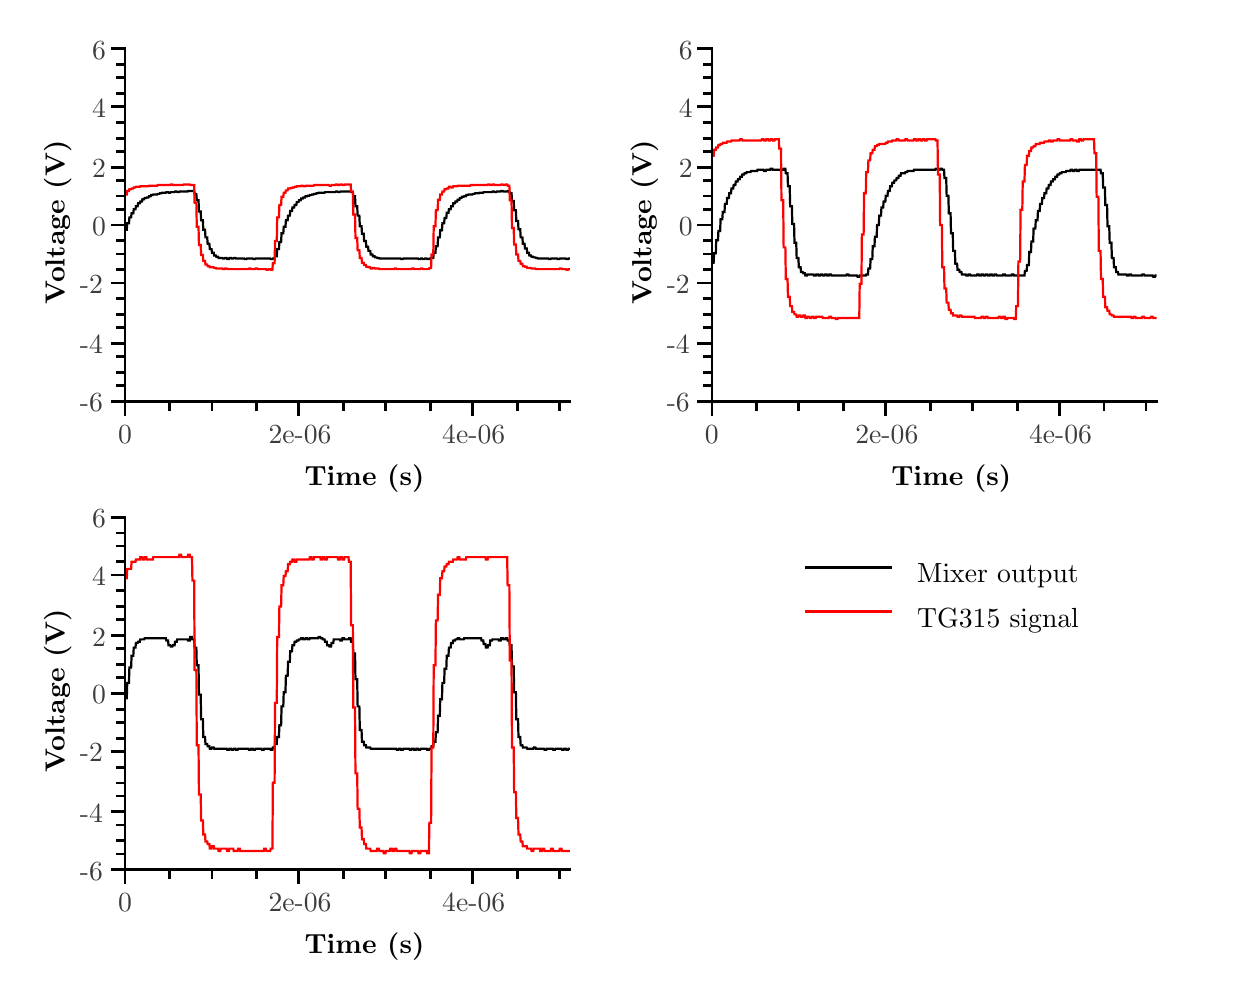
\begin{tikzpicture}{0pt}{0pt}{449pt}{359pt}
	\clip(0pt,359pt) -- (426.964pt,359pt) -- (426.964pt,17.6193pt) -- (0pt,17.6193pt) -- (0pt,359pt);
\begin{scope}
	\clip(35.1841pt,351.393pt) -- (195.89pt,351.393pt) -- (195.89pt,223.969pt) -- (35.1841pt,223.969pt) -- (35.1841pt,351.393pt);
	\color[rgb]{0,0,0}
	\draw[line width=0.8pt, line join=miter, line cap=rect](35.3412pt,285.982pt) -- (35.4983pt,285.982pt) -- (35.6554pt,285.982pt) -- (35.8124pt,285.982pt) -- (35.9695pt,288.318pt) -- (36.1266pt,288.318pt) -- (36.2837pt,288.318pt) -- (36.4408pt,288.318pt) -- (36.5979pt,288.318pt) -- (36.755pt,290.442pt) -- (36.9121pt,290.442pt) -- (37.0692pt,290.442pt) -- (37.2263pt,290.442pt) -- (37.3834pt,290.442pt) -- (37.5405pt,291.928pt) -- (37.6976pt,291.928pt) -- (37.8547pt,291.928pt) -- (38.0117pt,291.928pt) -- (38.1688pt,291.928pt) -- (38.3259pt,293.415pt) -- (38.483pt,293.415pt) -- (38.6401pt,293.415pt) -- (38.7972pt,293.415pt) -- (38.9543pt,293.415pt) -- (39.1114pt,294.477pt) -- (39.2685pt,294.477pt) -- (39.4256pt,294.477pt) -- (39.5827pt,294.477pt) -- (39.7398pt,294.477pt) -- (39.8969pt,295.539pt) -- (40.0539pt,295.539pt) -- (40.211pt,295.539pt) -- (40.3681pt,295.539pt) -- (40.5252pt,295.539pt) -- (40.6823pt,296.176pt) -- (40.8394pt,296.176pt) -- (40.9965pt,296.176pt) -- (41.1536pt,296.176pt) -- (41.3107pt,296.176pt) -- (41.4678pt,297.025pt) -- (41.6249pt,297.025pt) -- (41.782pt,297.025pt) -- (41.9391pt,297.025pt) -- (42.0962pt,297.025pt) -- (42.2532pt,297.45pt) -- (42.4103pt,297.45pt) -- (42.5674pt,297.45pt) -- (42.7245pt,297.45pt) -- (42.8816pt,297.45pt) -- (43.0387pt,297.662pt) -- (43.1958pt,297.662pt) -- (43.3529pt,297.662pt) -- (43.51pt,297.662pt) -- (43.6671pt,297.662pt) -- (43.8242pt,298.087pt) -- (43.9813pt,298.087pt) -- (44.1384pt,298.087pt) -- (44.2954pt,298.087pt) -- (44.4525pt,298.087pt) -- (44.6096pt,298.512pt) -- (44.7667pt,298.512pt) -- (44.9238pt,298.512pt) -- (45.0809pt,298.512pt) -- (45.238pt,298.512pt) -- (45.3951pt,298.724pt) -- (45.5522pt,298.724pt) -- (45.7093pt,298.724pt) -- (45.8664pt,298.724pt) -- (46.0235pt,298.724pt) -- (46.1806pt,298.724pt) -- (46.3376pt,298.724pt) -- (46.4947pt,298.724pt) -- (46.6518pt,298.724pt) -- (46.8089pt,298.724pt) -- (46.966pt,298.937pt) -- (47.1231pt,298.937pt) -- (47.2802pt,298.937pt) -- (47.4373pt,298.937pt) -- (47.5944pt,298.937pt) -- (47.7515pt,299.149pt) -- (47.9086pt,299.149pt) -- (48.0657pt,299.149pt) -- (48.2228pt,299.149pt) -- (48.3799pt,299.149pt) -- (48.5369pt,299.361pt) -- (48.694pt,299.361pt) -- (48.8511pt,299.361pt) -- (49.0082pt,299.361pt) -- (49.1653pt,299.361pt) -- (49.3224pt,299.361pt) -- (49.4795pt,299.361pt) -- (49.6366pt,299.361pt) -- (49.7937pt,299.361pt) -- (49.9508pt,299.361pt) -- (50.1079pt,299.574pt) -- (50.265pt,299.574pt) -- (50.4221pt,299.574pt) -- (50.5791pt,299.574pt) -- (50.7362pt,299.574pt) -- (50.8933pt,299.361pt) -- (51.0504pt,299.361pt) -- (51.2075pt,299.361pt) -- (51.3646pt,299.361pt) -- (51.5217pt,299.361pt) -- (51.6788pt,299.574pt) -- (51.8359pt,299.574pt) -- (51.993pt,299.574pt) -- (52.1501pt,299.574pt) -- (52.3072pt,299.574pt) -- (52.4643pt,299.574pt) -- (52.6213pt,299.574pt) -- (52.7784pt,299.574pt) -- (52.9355pt,299.574pt) -- (53.0926pt,299.574pt) -- (53.2497pt,299.786pt) -- (53.4068pt,299.786pt) -- (53.5639pt,299.786pt) -- (53.721pt,299.786pt) -- (53.8781pt,299.786pt) -- (54.0352pt,299.574pt) -- (54.1923pt,299.574pt) -- (54.3494pt,299.574pt) -- (54.5065pt,299.574pt) -- (54.6636pt,299.574pt) -- (54.8206pt,299.786pt) -- (54.9777pt,299.786pt) -- (55.1348pt,299.786pt) -- (55.2919pt,299.786pt) -- (55.449pt,299.786pt) -- (55.6061pt,299.786pt) -- (55.7632pt,299.786pt) -- (55.9203pt,299.786pt) -- (56.0774pt,299.786pt) -- (56.2345pt,299.786pt) -- (56.3916pt,299.786pt) -- (56.5487pt,299.786pt) -- (56.7058pt,299.786pt) -- (56.8628pt,299.786pt) -- (57.0199pt,299.786pt) -- (57.177pt,299.786pt) -- (57.3341pt,299.786pt) -- (57.4912pt,299.786pt) -- (57.6483pt,299.786pt) -- (57.8054pt,299.786pt) -- (57.9625pt,299.999pt) -- (58.1196pt,299.999pt) -- (58.2767pt,299.999pt) -- (58.4338pt,299.999pt) -- (58.5909pt,299.999pt) -- (58.748pt,299.999pt) -- (58.9051pt,299.999pt) -- (59.0621pt,299.999pt) -- (59.2192pt,299.999pt) -- (59.3763pt,299.999pt) -- (59.5334pt,299.999pt) -- (59.6905pt,299.999pt) -- (59.8476pt,299.999pt) -- (60.0047pt,299.999pt) -- (60.1618pt,299.999pt) -- (60.3189pt,298.937pt) -- (60.476pt,298.937pt) -- (60.6331pt,298.937pt) -- (60.7902pt,298.937pt) -- (60.9473pt,298.937pt) -- (61.1043pt,296.601pt) -- (61.2614pt,296.601pt) -- (61.4185pt,296.601pt) -- (61.5756pt,296.601pt) -- (61.7327pt,296.601pt) -- (61.8898pt,292.565pt) -- (62.0469pt,292.565pt) -- (62.204pt,292.565pt) -- (62.3611pt,292.565pt) -- (62.5182pt,292.565pt) -- (62.6753pt,289.38pt) -- (62.8324pt,289.38pt) -- (62.9895pt,289.38pt) -- (63.1465pt,289.38pt) -- (63.3036pt,289.38pt) -- (63.4607pt,285.982pt) -- (63.6178pt,285.982pt) -- (63.7749pt,285.982pt) -- (63.932pt,285.982pt) -- (64.0891pt,285.982pt) -- (64.2462pt,283.221pt) -- (64.4033pt,283.221pt) -- (64.5604pt,283.221pt) -- (64.7175pt,283.221pt) -- (64.8746pt,283.221pt) -- (65.0317pt,280.885pt) -- (65.1888pt,280.885pt) -- (65.3458pt,280.885pt) -- (65.5029pt,280.885pt) -- (65.66pt,280.885pt) -- (65.8171pt,278.974pt) -- (65.9742pt,278.974pt) -- (66.1313pt,278.974pt) -- (66.2884pt,278.974pt) -- (66.4455pt,278.974pt) -- (66.6026pt,277.699pt) -- (66.7597pt,277.699pt) -- (66.9168pt,277.699pt) -- (67.0739pt,277.699pt) -- (67.231pt,277.699pt) -- (67.388pt,276.638pt) -- (67.5451pt,276.638pt) -- (67.7022pt,276.638pt) -- (67.8593pt,276.638pt) -- (68.0164pt,276.638pt) -- (68.1735pt,276.213pt) -- (68.3306pt,276.213pt) -- (68.4877pt,276.213pt) -- (68.6448pt,276.213pt) -- (68.8019pt,276.213pt) -- (68.959pt,275.788pt) -- (69.1161pt,275.788pt) -- (69.2732pt,275.788pt) -- (69.4303pt,275.788pt) -- (69.5873pt,275.788pt) -- (69.7444pt,275.788pt) -- (69.9015pt,275.788pt) -- (70.0586pt,275.788pt) -- (70.2157pt,275.788pt) -- (70.3728pt,275.788pt) -- (70.5299pt,275.576pt) -- (70.687pt,275.576pt) -- (70.8441pt,275.576pt) -- (71.0012pt,275.576pt) -- (71.1583pt,275.576pt) -- (71.3154pt,275.788pt) -- (71.4725pt,275.788pt) -- (71.6295pt,275.788pt) -- (71.7866pt,275.788pt) -- (71.9437pt,275.788pt) -- (72.1008pt,275.363pt) -- (72.2579pt,275.363pt) -- (72.415pt,275.363pt) -- (72.5721pt,275.363pt) -- (72.7292pt,275.363pt) -- (72.8863pt,275.788pt) -- (73.0434pt,275.788pt) -- (73.2005pt,275.788pt) -- (73.3576pt,275.788pt) -- (73.5147pt,275.788pt) -- (73.6717pt,275.576pt) -- (73.8288pt,275.576pt) -- (73.9859pt,275.576pt) -- (74.143pt,275.576pt) -- (74.3001pt,275.576pt) -- (74.4572pt,275.788pt) -- (74.6143pt,275.788pt) -- (74.7714pt,275.788pt) -- (74.9285pt,275.788pt) -- (75.0856pt,275.788pt) -- (75.2427pt,275.576pt) -- (75.3998pt,275.576pt) -- (75.5569pt,275.576pt) -- (75.714pt,275.576pt) -- (75.871pt,275.576pt) -- (76.0281pt,275.576pt) -- (76.1852pt,275.576pt) -- (76.3423pt,275.576pt) -- (76.4994pt,275.576pt) -- (76.6565pt,275.576pt) -- (76.8136pt,275.576pt) -- (76.9707pt,275.576pt) -- (77.1278pt,275.576pt) -- (77.2849pt,275.576pt) -- (77.442pt,275.576pt) -- (77.5991pt,275.576pt) -- (77.7562pt,275.576pt) -- (77.9132pt,275.576pt) -- (78.0703pt,275.576pt) -- (78.2274pt,275.576pt) -- (78.3845pt,275.363pt) -- (78.5416pt,275.363pt) -- (78.6987pt,275.363pt) -- (78.8558pt,275.363pt) -- (79.0129pt,275.363pt) -- (79.17pt,275.576pt) -- (79.3271pt,275.576pt) -- (79.4842pt,275.576pt) -- (79.6413pt,275.576pt) -- (79.7984pt,275.576pt) -- (79.9554pt,275.576pt) -- (80.1125pt,275.576pt) -- (80.2696pt,275.576pt) -- (80.4267pt,275.576pt) -- (80.5838pt,275.576pt) -- (80.7409pt,275.576pt) -- (80.898pt,275.576pt) -- (81.0551pt,275.576pt) -- (81.2122pt,275.576pt) -- (81.3693pt,275.576pt) -- (81.5264pt,275.363pt) -- (81.6835pt,275.363pt) -- (81.8406pt,275.363pt) -- (81.9977pt,275.363pt) -- (82.1547pt,275.363pt) -- (82.3118pt,275.576pt) -- (82.4689pt,275.576pt) -- (82.626pt,275.576pt) -- (82.7831pt,275.576pt) -- (82.9402pt,275.576pt) -- (83.0973pt,275.576pt) -- (83.2544pt,275.576pt) -- (83.4115pt,275.576pt) -- (83.5686pt,275.576pt) -- (83.7257pt,275.576pt) -- (83.8828pt,275.576pt) -- (84.0399pt,275.576pt) -- (84.1969pt,275.576pt) -- (84.354pt,275.576pt) -- (84.5111pt,275.576pt) -- (84.6682pt,275.576pt) -- (84.8253pt,275.576pt) -- (84.9824pt,275.576pt) -- (85.1395pt,275.576pt) -- (85.2966pt,275.576pt) -- (85.4537pt,275.576pt) -- (85.6108pt,275.576pt) -- (85.7679pt,275.576pt) -- (85.925pt,275.576pt) -- (86.0821pt,275.576pt) -- (86.2392pt,275.576pt) -- (86.3962pt,275.576pt) -- (86.5533pt,275.576pt) -- (86.7104pt,275.576pt) -- (86.8675pt,275.576pt) -- (87.0246pt,275.576pt) -- (87.1817pt,275.576pt) -- (87.3388pt,275.576pt) -- (87.4959pt,275.576pt) -- (87.653pt,275.576pt) -- (87.8101pt,275.363pt) -- (87.9672pt,275.363pt) -- (88.1243pt,275.363pt) -- (88.2814pt,275.363pt) -- (88.4384pt,275.363pt) -- (88.5955pt,275.576pt) -- (88.7526pt,275.576pt) -- (88.9097pt,275.576pt) -- (89.0668pt,275.576pt) -- (89.2239pt,275.576pt) -- (89.381pt,276.425pt) -- (89.5381pt,276.425pt) -- (89.6952pt,276.425pt) -- (89.8523pt,276.425pt) -- (90.0094pt,276.425pt) -- (90.1665pt,278.974pt) -- (90.3236pt,278.974pt) -- (90.4806pt,278.974pt) -- (90.6377pt,278.974pt) -- (90.7948pt,278.974pt) -- (90.9519pt,281.522pt) -- (91.109pt,281.522pt) -- (91.2661pt,281.522pt) -- (91.4232pt,281.522pt) -- (91.5803pt,281.522pt) -- (91.7374pt,284.708pt) -- (91.8945pt,284.708pt) -- (92.0516pt,284.708pt) -- (92.2087pt,284.708pt) -- (92.3658pt,284.708pt) -- (92.5229pt,287.044pt) -- (92.6799pt,287.044pt) -- (92.837pt,287.044pt) -- (92.9941pt,287.044pt) -- (93.1512pt,287.044pt) -- (93.3083pt,289.38pt) -- (93.4654pt,289.38pt) -- (93.6225pt,289.38pt) -- (93.7796pt,289.38pt) -- (93.9367pt,289.38pt) -- (94.0938pt,291.079pt) -- (94.2509pt,291.079pt) -- (94.408pt,291.079pt) -- (94.5651pt,291.079pt) -- (94.7221pt,291.079pt) -- (94.8792pt,292.778pt) -- (95.0363pt,292.778pt) -- (95.1934pt,292.778pt) -- (95.3505pt,292.778pt) -- (95.5076pt,292.778pt) -- (95.6647pt,294.052pt) -- (95.8218pt,294.052pt) -- (95.9789pt,294.052pt) -- (96.136pt,294.052pt) -- (96.2931pt,294.052pt) -- (96.4502pt,294.902pt) -- (96.6073pt,294.902pt) -- (96.7644pt,294.902pt) -- (96.9214pt,294.902pt) -- (97.0785pt,294.902pt) -- (97.2356pt,295.963pt) -- (97.3927pt,295.963pt) -- (97.5498pt,295.963pt) -- (97.7069pt,295.963pt) -- (97.864pt,295.963pt) -- (98.0211pt,296.601pt) -- (98.1782pt,296.601pt) -- (98.3353pt,296.601pt) -- (98.4924pt,296.601pt) -- (98.6495pt,296.601pt) -- (98.8066pt,297.238pt) -- (98.9636pt,297.238pt) -- (99.1207pt,297.238pt) -- (99.2778pt,297.238pt) -- (99.4349pt,297.238pt) -- (99.592pt,297.662pt) -- (99.7491pt,297.662pt) -- (99.9062pt,297.662pt) -- (100.063pt,297.662pt) -- (100.22pt,297.662pt) -- (100.377pt,298.087pt) -- (100.535pt,298.087pt) -- (100.692pt,298.087pt) -- (100.849pt,298.087pt) -- (101.006pt,298.087pt) -- (101.163pt,298.3pt) -- (101.32pt,298.3pt) -- (101.477pt,298.3pt) -- (101.634pt,298.3pt) -- (101.791pt,298.3pt) -- (101.948pt,298.512pt) -- (102.105pt,298.512pt) -- (102.263pt,298.512pt) -- (102.42pt,298.512pt) -- (102.577pt,298.512pt) -- (102.734pt,298.724pt) -- (102.891pt,298.724pt) -- (103.048pt,298.724pt) -- (103.205pt,298.724pt) -- (103.362pt,298.724pt) -- (103.519pt,298.937pt) -- (103.676pt,298.937pt) -- (103.834pt,298.937pt) -- (103.991pt,298.937pt) -- (104.148pt,298.937pt) -- (104.305pt,299.149pt) -- (104.462pt,299.149pt) -- (104.619pt,299.149pt) -- (104.776pt,299.149pt) -- (104.933pt,299.149pt) -- (105.09pt,299.361pt) -- (105.247pt,299.361pt) -- (105.404pt,299.361pt) -- (105.562pt,299.361pt) -- (105.719pt,299.361pt) -- (105.876pt,299.361pt) -- (106.033pt,299.361pt) -- (106.19pt,299.361pt) -- (106.347pt,299.361pt) -- (106.504pt,299.361pt) -- (106.661pt,299.361pt) -- (106.818pt,299.361pt) -- (106.975pt,299.361pt) -- (107.132pt,299.361pt) -- (107.29pt,299.361pt) -- (107.447pt,299.574pt) -- (107.604pt,299.574pt) -- (107.761pt,299.574pt) -- (107.918pt,299.574pt) -- (108.075pt,299.574pt) -- (108.232pt,299.574pt) -- (108.389pt,299.574pt) -- (108.546pt,299.574pt) -- (108.703pt,299.574pt) -- (108.86pt,299.574pt) -- (109.018pt,299.574pt) -- (109.175pt,299.574pt) -- (109.332pt,299.574pt) -- (109.489pt,299.574pt) -- (109.646pt,299.574pt) -- (109.803pt,299.574pt) -- (109.96pt,299.574pt) -- (110.117pt,299.574pt) -- (110.274pt,299.574pt) -- (110.431pt,299.574pt) -- (110.588pt,299.574pt) -- (110.746pt,299.574pt) -- (110.903pt,299.574pt) -- (111.06pt,299.574pt) -- (111.217pt,299.574pt) -- (111.374pt,299.786pt) -- (111.531pt,299.786pt) -- (111.688pt,299.786pt) -- (111.845pt,299.786pt) -- (112.002pt,299.786pt) -- (112.159pt,299.574pt) -- (112.317pt,299.574pt) -- (112.474pt,299.574pt) -- (112.631pt,299.574pt) -- (112.788pt,299.574pt) -- (112.945pt,299.786pt) -- (113.102pt,299.786pt) -- (113.259pt,299.786pt) -- (113.416pt,299.786pt) -- (113.573pt,299.786pt) -- (113.73pt,299.786pt) -- (113.887pt,299.786pt) -- (114.045pt,299.786pt) -- (114.202pt,299.786pt) -- (114.359pt,299.786pt) -- (114.516pt,299.786pt) -- (114.673pt,299.786pt) -- (114.83pt,299.786pt) -- (114.987pt,299.786pt) -- (115.144pt,299.786pt) -- (115.301pt,299.786pt) -- (115.458pt,299.786pt) -- (115.615pt,299.786pt) -- (115.773pt,299.786pt) -- (115.93pt,299.786pt) -- (116.087pt,299.786pt) -- (116.244pt,299.786pt) -- (116.401pt,299.786pt) -- (116.558pt,299.786pt) -- (116.715pt,299.786pt) -- (116.872pt,299.574pt) -- (117.029pt,299.574pt) -- (117.186pt,299.574pt) -- (117.343pt,299.574pt) -- (117.501pt,299.574pt) -- (117.658pt,298.087pt) -- (117.815pt,298.087pt) -- (117.972pt,298.087pt) -- (118.129pt,298.087pt) -- (118.286pt,298.087pt) -- (118.443pt,294.477pt) -- (118.6pt,294.477pt) -- (118.757pt,294.477pt) -- (118.914pt,294.477pt) -- (119.071pt,294.477pt) -- (119.229pt,291.079pt) -- (119.386pt,291.079pt) -- (119.543pt,291.079pt) -- (119.7pt,291.079pt) -- (119.857pt,291.079pt) -- (120.014pt,287.256pt) -- (120.171pt,287.256pt) -- (120.328pt,287.256pt) -- (120.485pt,287.256pt) -- (120.642pt,287.256pt) -- (120.8pt,284.495pt) -- (120.957pt,284.495pt) -- (121.114pt,284.495pt) -- (121.271pt,284.495pt) -- (121.428pt,284.495pt) -- (121.585pt,281.947pt) -- (121.742pt,281.947pt) -- (121.899pt,281.947pt) -- (122.056pt,281.947pt) -- (122.213pt,281.947pt) -- (122.37pt,279.823pt) -- (122.528pt,279.823pt) -- (122.685pt,279.823pt) -- (122.842pt,279.823pt) -- (122.999pt,279.823pt) -- (123.156pt,278.337pt) -- (123.313pt,278.337pt) -- (123.47pt,278.337pt) -- (123.627pt,278.337pt) -- (123.784pt,278.337pt) -- (123.941pt,277.062pt) -- (124.098pt,277.062pt) -- (124.256pt,277.062pt) -- (124.413pt,277.062pt) -- (124.57pt,277.062pt) -- (124.727pt,276.425pt) -- (124.884pt,276.425pt) -- (125.041pt,276.425pt) -- (125.198pt,276.425pt) -- (125.355pt,276.425pt) -- (125.512pt,276pt) -- (125.669pt,276pt) -- (125.826pt,276pt) -- (125.984pt,276pt) -- (126.141pt,276pt) -- (126.298pt,275.788pt) -- (126.455pt,275.788pt) -- (126.612pt,275.788pt) -- (126.769pt,275.788pt) -- (126.926pt,275.788pt) -- (127.083pt,275.576pt) -- (127.24pt,275.576pt) -- (127.397pt,275.576pt) -- (127.554pt,275.576pt) -- (127.712pt,275.576pt) -- (127.869pt,275.576pt) -- (128.026pt,275.576pt) -- (128.183pt,275.576pt) -- (128.34pt,275.576pt) -- (128.497pt,275.576pt) -- (128.654pt,275.576pt) -- (128.811pt,275.576pt) -- (128.968pt,275.576pt) -- (129.125pt,275.576pt) -- (129.283pt,275.576pt) -- (129.44pt,275.576pt) -- (129.597pt,275.576pt) -- (129.754pt,275.576pt) -- (129.911pt,275.576pt) -- (130.068pt,275.576pt) -- (130.225pt,275.576pt) -- (130.382pt,275.576pt) -- (130.539pt,275.576pt) -- (130.696pt,275.576pt) -- (130.853pt,275.576pt) -- (131.011pt,275.576pt) -- (131.168pt,275.576pt) -- (131.325pt,275.576pt) -- (131.482pt,275.576pt) -- (131.639pt,275.576pt) -- (131.796pt,275.576pt) -- (131.953pt,275.576pt) -- (132.11pt,275.576pt) -- (132.267pt,275.576pt) -- (132.424pt,275.576pt) -- (132.581pt,275.576pt) -- (132.739pt,275.576pt) -- (132.896pt,275.576pt) -- (133.053pt,275.576pt) -- (133.21pt,275.576pt) -- (133.367pt,275.576pt) -- (133.524pt,275.576pt) -- (133.681pt,275.576pt) -- (133.838pt,275.576pt) -- (133.995pt,275.576pt) -- (134.152pt,275.576pt) -- (134.309pt,275.576pt) -- (134.467pt,275.576pt) -- (134.624pt,275.576pt) -- (134.781pt,275.576pt) -- (134.938pt,275.363pt) -- (135.095pt,275.363pt) -- (135.252pt,275.363pt) -- (135.409pt,275.363pt) -- (135.566pt,275.363pt) -- (135.723pt,275.576pt) -- (135.88pt,275.576pt) -- (136.037pt,275.576pt) -- (136.195pt,275.576pt) -- (136.352pt,275.576pt) -- (136.509pt,275.576pt) -- (136.666pt,275.576pt) -- (136.823pt,275.576pt) -- (136.98pt,275.576pt) -- (137.137pt,275.576pt) -- (137.294pt,275.576pt) -- (137.451pt,275.576pt) -- (137.608pt,275.576pt) -- (137.766pt,275.576pt) -- (137.923pt,275.576pt) -- (138.08pt,275.576pt) -- (138.237pt,275.576pt) -- (138.394pt,275.576pt) -- (138.551pt,275.576pt) -- (138.708pt,275.576pt) -- (138.865pt,275.576pt) -- (139.022pt,275.576pt) -- (139.179pt,275.576pt) -- (139.336pt,275.576pt) -- (139.494pt,275.576pt) -- (139.651pt,275.576pt) -- (139.808pt,275.576pt) -- (139.965pt,275.576pt) -- (140.122pt,275.576pt) -- (140.279pt,275.576pt) -- (140.436pt,275.576pt) -- (140.593pt,275.576pt) -- (140.75pt,275.576pt) -- (140.907pt,275.576pt) -- (141.064pt,275.576pt) -- (141.222pt,275.363pt) -- (141.379pt,275.363pt) -- (141.536pt,275.363pt) -- (141.693pt,275.363pt) -- (141.85pt,275.363pt) -- (142.007pt,275.576pt) -- (142.164pt,275.576pt) -- (142.321pt,275.576pt) -- (142.478pt,275.576pt) -- (142.635pt,275.576pt) -- (142.792pt,275.363pt) -- (142.95pt,275.363pt) -- (143.107pt,275.363pt) -- (143.264pt,275.363pt) -- (143.421pt,275.363pt) -- (143.578pt,275.576pt) -- (143.735pt,275.576pt) -- (143.892pt,275.576pt) -- (144.049pt,275.576pt) -- (144.206pt,275.576pt) -- (144.363pt,275.363pt) -- (144.52pt,275.363pt) -- (144.678pt,275.363pt) -- (144.835pt,275.363pt) -- (144.992pt,275.363pt) -- (145.149pt,275.576pt) -- (145.306pt,275.576pt) -- (145.463pt,275.576pt) -- (145.62pt,275.576pt) -- (145.777pt,275.576pt) -- (145.934pt,275.788pt) -- (146.091pt,275.788pt) -- (146.248pt,275.788pt) -- (146.406pt,275.788pt) -- (146.563pt,275.788pt) -- (146.72pt,277.699pt) -- (146.877pt,277.699pt) -- (147.034pt,277.699pt) -- (147.191pt,277.699pt) -- (147.348pt,277.699pt) -- (147.505pt,280.036pt) -- (147.662pt,280.036pt) -- (147.819pt,280.036pt) -- (147.977pt,280.036pt) -- (148.134pt,280.036pt) -- (148.291pt,283.221pt) -- (148.448pt,283.221pt) -- (148.605pt,283.221pt) -- (148.762pt,283.221pt) -- (148.919pt,283.221pt) -- (149.076pt,285.77pt) -- (149.233pt,285.77pt) -- (149.39pt,285.77pt) -- (149.547pt,285.77pt) -- (149.705pt,285.77pt) -- (149.862pt,288.318pt) -- (150.019pt,288.318pt) -- (150.176pt,288.318pt) -- (150.333pt,288.318pt) -- (150.49pt,288.318pt) -- (150.647pt,290.229pt) -- (150.804pt,290.229pt) -- (150.961pt,290.229pt) -- (151.118pt,290.229pt) -- (151.275pt,290.229pt) -- (151.433pt,292.141pt) -- (151.59pt,292.141pt) -- (151.747pt,292.141pt) -- (151.904pt,292.141pt) -- (152.061pt,292.141pt) -- (152.218pt,293.415pt) -- (152.375pt,293.415pt) -- (152.532pt,293.415pt) -- (152.689pt,293.415pt) -- (152.846pt,293.415pt) -- (153.003pt,294.477pt) -- (153.161pt,294.477pt) -- (153.318pt,294.477pt) -- (153.475pt,294.477pt) -- (153.632pt,294.477pt) -- (153.789pt,295.539pt) -- (153.946pt,295.539pt) -- (154.103pt,295.539pt) -- (154.26pt,295.539pt) -- (154.417pt,295.539pt) -- (154.574pt,296.176pt) -- (154.731pt,296.176pt) -- (154.889pt,296.176pt) -- (155.046pt,296.176pt) -- (155.203pt,296.176pt) -- (155.36pt,296.813pt) -- (155.517pt,296.813pt) -- (155.674pt,296.813pt) -- (155.831pt,296.813pt) -- (155.988pt,296.813pt) -- (156.145pt,297.45pt) -- (156.302pt,297.45pt) -- (156.46pt,297.45pt) -- (156.617pt,297.45pt) -- (156.774pt,297.45pt) -- (156.931pt,297.875pt) -- (157.088pt,297.875pt) -- (157.245pt,297.875pt) -- (157.402pt,297.875pt) -- (157.559pt,297.875pt) -- (157.716pt,298.087pt) -- (157.873pt,298.087pt) -- (158.03pt,298.087pt) -- (158.188pt,298.087pt) -- (158.345pt,298.087pt) -- (158.502pt,298.512pt) -- (158.659pt,298.512pt) -- (158.816pt,298.512pt) -- (158.973pt,298.512pt) -- (159.13pt,298.512pt) -- (159.287pt,298.724pt) -- (159.444pt,298.724pt) -- (159.601pt,298.724pt) -- (159.758pt,298.724pt) -- (159.916pt,298.724pt) -- (160.073pt,298.724pt) -- (160.23pt,298.724pt) -- (160.387pt,298.724pt) -- (160.544pt,298.724pt) -- (160.701pt,298.724pt) -- (160.858pt,298.937pt) -- (161.015pt,298.937pt) -- (161.172pt,298.937pt) -- (161.329pt,298.937pt) -- (161.486pt,298.937pt) -- (161.644pt,299.149pt) -- (161.801pt,299.149pt) -- (161.958pt,299.149pt) -- (162.115pt,299.149pt) -- (162.272pt,299.149pt) -- (162.429pt,299.149pt) -- (162.586pt,299.149pt) -- (162.743pt,299.149pt) -- (162.9pt,299.149pt) -- (163.057pt,299.149pt) -- (163.214pt,299.361pt) -- (163.372pt,299.361pt) -- (163.529pt,299.361pt) -- (163.686pt,299.361pt) -- (163.843pt,299.361pt) -- (164pt,299.361pt) -- (164.157pt,299.361pt) -- (164.314pt,299.361pt) -- (164.471pt,299.361pt) -- (164.628pt,299.361pt) -- (164.785pt,299.574pt) -- (164.943pt,299.574pt) -- (165.1pt,299.574pt) -- (165.257pt,299.574pt) -- (165.414pt,299.574pt) -- (165.571pt,299.574pt) -- (165.728pt,299.574pt) -- (165.885pt,299.574pt) -- (166.042pt,299.574pt) -- (166.199pt,299.574pt) -- (166.356pt,299.574pt) -- (166.513pt,299.574pt) -- (166.671pt,299.574pt) -- (166.828pt,299.574pt) -- (166.985pt,299.574pt) -- (167.142pt,299.574pt) -- (167.299pt,299.574pt) -- (167.456pt,299.574pt) -- (167.613pt,299.574pt) -- (167.77pt,299.574pt) -- (167.927pt,299.786pt) -- (168.084pt,299.786pt) -- (168.241pt,299.786pt) -- (168.399pt,299.786pt) -- (168.556pt,299.786pt) -- (168.713pt,299.574pt) -- (168.87pt,299.574pt) -- (169.027pt,299.574pt) -- (169.184pt,299.574pt) -- (169.341pt,299.574pt) -- (169.498pt,299.786pt) -- (169.655pt,299.786pt) -- (169.812pt,299.786pt) -- (169.969pt,299.786pt) -- (170.127pt,299.786pt) -- (170.284pt,299.786pt) -- (170.441pt,299.786pt) -- (170.598pt,299.786pt) -- (170.755pt,299.786pt) -- (170.912pt,299.786pt) -- (171.069pt,299.999pt) -- (171.226pt,299.999pt) -- (171.383pt,299.999pt) -- (171.54pt,299.999pt) -- (171.697pt,299.999pt) -- (171.855pt,299.786pt) -- (172.012pt,299.786pt) -- (172.169pt,299.786pt) -- (172.326pt,299.786pt) -- (172.483pt,299.786pt) -- (172.64pt,299.786pt) -- (172.797pt,299.786pt) -- (172.954pt,299.786pt) -- (173.111pt,299.786pt) -- (173.268pt,299.786pt) -- (173.426pt,299.999pt) -- (173.583pt,299.999pt) -- (173.74pt,299.999pt) -- (173.897pt,299.999pt) -- (174.054pt,299.999pt) -- (174.211pt,299.149pt) -- (174.368pt,299.149pt) -- (174.525pt,299.149pt) -- (174.682pt,299.149pt) -- (174.839pt,299.149pt) -- (174.996pt,296.388pt) -- (175.154pt,296.388pt) -- (175.311pt,296.388pt) -- (175.468pt,296.388pt) -- (175.625pt,296.388pt) -- (175.782pt,292.99pt) -- (175.939pt,292.99pt) -- (176.096pt,292.99pt) -- (176.253pt,292.99pt) -- (176.41pt,292.99pt) -- (176.567pt,289.168pt) -- (176.724pt,289.168pt) -- (176.882pt,289.168pt) -- (177.039pt,289.168pt) -- (177.196pt,289.168pt) -- (177.353pt,286.194pt) -- (177.51pt,286.194pt) -- (177.667pt,286.194pt) -- (177.824pt,286.194pt) -- (177.981pt,286.194pt) -- (178.138pt,283.221pt) -- (178.295pt,283.221pt) -- (178.452pt,283.221pt) -- (178.61pt,283.221pt) -- (178.767pt,283.221pt) -- (178.924pt,280.885pt) -- (179.081pt,280.885pt) -- (179.238pt,280.885pt) -- (179.395pt,280.885pt) -- (179.552pt,280.885pt) -- (179.709pt,279.186pt) -- (179.866pt,279.186pt) -- (180.023pt,279.186pt) -- (180.18pt,279.186pt) -- (180.338pt,279.186pt) -- (180.495pt,277.699pt) -- (180.652pt,277.699pt) -- (180.809pt,277.699pt) -- (180.966pt,277.699pt) -- (181.123pt,277.699pt) -- (181.28pt,276.638pt) -- (181.437pt,276.638pt) -- (181.594pt,276.638pt) -- (181.751pt,276.638pt) -- (181.909pt,276.638pt) -- (182.066pt,276.213pt) -- (182.223pt,276.213pt) -- (182.38pt,276.213pt) -- (182.537pt,276.213pt) -- (182.694pt,276.213pt) -- (182.851pt,276pt) -- (183.008pt,276pt) -- (183.165pt,276pt) -- (183.322pt,276pt) -- (183.479pt,276pt) -- (183.637pt,275.788pt) -- (183.794pt,275.788pt) -- (183.951pt,275.788pt) -- (184.108pt,275.788pt) -- (184.265pt,275.788pt) -- (184.422pt,275.576pt) -- (184.579pt,275.576pt) -- (184.736pt,275.576pt) -- (184.893pt,275.576pt) -- (185.05pt,275.576pt) -- (185.207pt,275.576pt) -- (185.365pt,275.576pt) -- (185.522pt,275.576pt) -- (185.679pt,275.576pt) -- (185.836pt,275.576pt) -- (185.993pt,275.576pt) -- (186.15pt,275.576pt) -- (186.307pt,275.576pt) -- (186.464pt,275.576pt) -- (186.621pt,275.576pt) -- (186.778pt,275.576pt) -- (186.935pt,275.576pt) -- (187.093pt,275.576pt) -- (187.25pt,275.576pt) -- (187.407pt,275.576pt) -- (187.564pt,275.576pt) -- (187.721pt,275.576pt) -- (187.878pt,275.576pt) -- (188.035pt,275.576pt) -- (188.192pt,275.576pt) -- (188.349pt,275.363pt) -- (188.506pt,275.363pt) -- (188.663pt,275.363pt) -- (188.821pt,275.363pt) -- (188.978pt,275.363pt) -- (189.135pt,275.576pt) -- (189.292pt,275.576pt) -- (189.449pt,275.576pt) -- (189.606pt,275.576pt) -- (189.763pt,275.576pt) -- (189.92pt,275.576pt) -- (190.077pt,275.576pt) -- (190.234pt,275.576pt) -- (190.391pt,275.576pt) -- (190.549pt,275.576pt) -- (190.706pt,275.576pt) -- (190.863pt,275.576pt) -- (191.02pt,275.576pt) -- (191.177pt,275.576pt) -- (191.334pt,275.576pt) -- (191.491pt,275.363pt) -- (191.648pt,275.363pt) -- (191.805pt,275.363pt) -- (191.962pt,275.363pt) -- (192.12pt,275.363pt) -- (192.277pt,275.576pt) -- (192.434pt,275.576pt) -- (192.591pt,275.576pt) -- (192.748pt,275.576pt) -- (192.905pt,275.576pt) -- (193.062pt,275.576pt) -- (193.219pt,275.576pt) -- (193.376pt,275.576pt) -- (193.533pt,275.576pt) -- (193.69pt,275.576pt) -- (193.848pt,275.576pt) -- (194.005pt,275.576pt) -- (194.162pt,275.576pt) -- (194.319pt,275.576pt) -- (194.476pt,275.576pt) -- (194.633pt,275.363pt) -- (194.79pt,275.363pt) -- (194.947pt,275.363pt) -- (195.104pt,275.363pt) -- (195.261pt,275.363pt) -- (195.418pt,275.576pt) -- (195.576pt,275.576pt) -- (195.733pt,275.576pt) -- (195.89pt,275.576pt);
	\color[rgb]{1,0,0}
	\draw[line width=0.8pt, line join=miter, line cap=rect](35.3412pt,298.724pt) -- (35.4983pt,298.724pt) -- (35.6554pt,298.724pt) -- (35.8124pt,298.724pt) -- (35.9695pt,299.999pt) -- (36.1266pt,299.999pt) -- (36.2837pt,299.999pt) -- (36.4408pt,299.999pt) -- (36.5979pt,299.999pt) -- (36.755pt,300.636pt) -- (36.9121pt,300.636pt) -- (37.0692pt,300.636pt) -- (37.2263pt,300.636pt) -- (37.3834pt,300.636pt) -- (37.5405pt,300.848pt) -- (37.6976pt,300.848pt) -- (37.8547pt,300.848pt) -- (38.0117pt,300.848pt) -- (38.1688pt,300.848pt) -- (38.3259pt,301.273pt) -- (38.483pt,301.273pt) -- (38.6401pt,301.273pt) -- (38.7972pt,301.273pt) -- (38.9543pt,301.273pt) -- (39.1114pt,301.485pt) -- (39.2685pt,301.485pt) -- (39.4256pt,301.485pt) -- (39.5827pt,301.485pt) -- (39.7398pt,301.485pt) -- (39.8969pt,301.485pt) -- (40.0539pt,301.485pt) -- (40.211pt,301.485pt) -- (40.3681pt,301.485pt) -- (40.5252pt,301.485pt) -- (40.6823pt,301.697pt) -- (40.8394pt,301.697pt) -- (40.9965pt,301.697pt) -- (41.1536pt,301.697pt) -- (41.3107pt,301.697pt) -- (41.4678pt,301.697pt) -- (41.6249pt,301.697pt) -- (41.782pt,301.697pt) -- (41.9391pt,301.697pt) -- (42.0962pt,301.697pt) -- (42.2532pt,301.697pt) -- (42.4103pt,301.697pt) -- (42.5674pt,301.697pt) -- (42.7245pt,301.697pt) -- (42.8816pt,301.697pt) -- (43.0387pt,301.697pt) -- (43.1958pt,301.697pt) -- (43.3529pt,301.697pt) -- (43.51pt,301.697pt) -- (43.6671pt,301.697pt) -- (43.8242pt,301.91pt) -- (43.9813pt,301.91pt) -- (44.1384pt,301.91pt) -- (44.2954pt,301.91pt) -- (44.4525pt,301.91pt) -- (44.6096pt,301.91pt) -- (44.7667pt,301.91pt) -- (44.9238pt,301.91pt) -- (45.0809pt,301.91pt) -- (45.238pt,301.91pt) -- (45.3951pt,301.91pt) -- (45.5522pt,301.91pt) -- (45.7093pt,301.91pt) -- (45.8664pt,301.91pt) -- (46.0235pt,301.91pt) -- (46.1806pt,301.91pt) -- (46.3376pt,301.91pt) -- (46.4947pt,301.91pt) -- (46.6518pt,301.91pt) -- (46.8089pt,301.91pt) -- (46.966pt,302.122pt) -- (47.1231pt,302.122pt) -- (47.2802pt,302.122pt) -- (47.4373pt,302.122pt) -- (47.5944pt,302.122pt) -- (47.7515pt,302.122pt) -- (47.9086pt,302.122pt) -- (48.0657pt,302.122pt) -- (48.2228pt,302.122pt) -- (48.3799pt,302.122pt) -- (48.5369pt,302.122pt) -- (48.694pt,302.122pt) -- (48.8511pt,302.122pt) -- (49.0082pt,302.122pt) -- (49.1653pt,302.122pt) -- (49.3224pt,302.122pt) -- (49.4795pt,302.122pt) -- (49.6366pt,302.122pt) -- (49.7937pt,302.122pt) -- (49.9508pt,302.122pt) -- (50.1079pt,302.122pt) -- (50.265pt,302.122pt) -- (50.4221pt,302.122pt) -- (50.5791pt,302.122pt) -- (50.7362pt,302.122pt) -- (50.8933pt,302.122pt) -- (51.0504pt,302.122pt) -- (51.2075pt,302.122pt) -- (51.3646pt,302.122pt) -- (51.5217pt,302.122pt) -- (51.6788pt,302.335pt) -- (51.8359pt,302.335pt) -- (51.993pt,302.335pt) -- (52.1501pt,302.335pt) -- (52.3072pt,302.335pt) -- (52.4643pt,302.122pt) -- (52.6213pt,302.122pt) -- (52.7784pt,302.122pt) -- (52.9355pt,302.122pt) -- (53.0926pt,302.122pt) -- (53.2497pt,302.122pt) -- (53.4068pt,302.122pt) -- (53.5639pt,302.122pt) -- (53.721pt,302.122pt) -- (53.8781pt,302.122pt) -- (54.0352pt,302.122pt) -- (54.1923pt,302.122pt) -- (54.3494pt,302.122pt) -- (54.5065pt,302.122pt) -- (54.6636pt,302.122pt) -- (54.8206pt,302.122pt) -- (54.9777pt,302.122pt) -- (55.1348pt,302.122pt) -- (55.2919pt,302.122pt) -- (55.449pt,302.122pt) -- (55.6061pt,302.122pt) -- (55.7632pt,302.122pt) -- (55.9203pt,302.122pt) -- (56.0774pt,302.122pt) -- (56.2345pt,302.122pt) -- (56.3916pt,302.335pt) -- (56.5487pt,302.335pt) -- (56.7058pt,302.335pt) -- (56.8628pt,302.335pt) -- (57.0199pt,302.335pt) -- (57.177pt,302.335pt) -- (57.3341pt,302.335pt) -- (57.4912pt,302.335pt) -- (57.6483pt,302.335pt) -- (57.8054pt,302.335pt) -- (57.9625pt,302.335pt) -- (58.1196pt,302.335pt) -- (58.2767pt,302.335pt) -- (58.4338pt,302.335pt) -- (58.5909pt,302.335pt) -- (58.748pt,302.122pt) -- (58.9051pt,302.122pt) -- (59.0621pt,302.122pt) -- (59.2192pt,302.122pt) -- (59.3763pt,302.122pt) -- (59.5334pt,302.122pt) -- (59.6905pt,302.122pt) -- (59.8476pt,302.122pt) -- (60.0047pt,302.122pt) -- (60.1618pt,302.122pt) -- (60.3189pt,295.751pt) -- (60.476pt,295.751pt) -- (60.6331pt,295.751pt) -- (60.7902pt,295.751pt) -- (60.9473pt,295.751pt) -- (61.1043pt,287.044pt) -- (61.2614pt,287.044pt) -- (61.4185pt,287.044pt) -- (61.5756pt,287.044pt) -- (61.7327pt,287.044pt) -- (61.8898pt,280.46pt) -- (62.0469pt,280.46pt) -- (62.204pt,280.46pt) -- (62.3611pt,280.46pt) -- (62.5182pt,280.46pt) -- (62.6753pt,276.85pt) -- (62.8324pt,276.85pt) -- (62.9895pt,276.85pt) -- (63.1465pt,276.85pt) -- (63.3036pt,276.85pt) -- (63.4607pt,274.726pt) -- (63.6178pt,274.726pt) -- (63.7749pt,274.726pt) -- (63.932pt,274.726pt) -- (64.0891pt,274.726pt) -- (64.2462pt,273.452pt) -- (64.4033pt,273.452pt) -- (64.5604pt,273.452pt) -- (64.7175pt,273.452pt) -- (64.8746pt,273.452pt) -- (65.0317pt,272.815pt) -- (65.1888pt,272.815pt) -- (65.3458pt,272.815pt) -- (65.5029pt,272.815pt) -- (65.66pt,272.815pt) -- (65.8171pt,272.39pt) -- (65.9742pt,272.39pt) -- (66.1313pt,272.39pt) -- (66.2884pt,272.39pt) -- (66.4455pt,272.39pt) -- (66.6026pt,272.39pt) -- (66.7597pt,272.39pt) -- (66.9168pt,272.39pt) -- (67.0739pt,272.39pt) -- (67.231pt,272.39pt) -- (67.388pt,272.178pt) -- (67.5451pt,272.178pt) -- (67.7022pt,272.178pt) -- (67.8593pt,272.178pt) -- (68.0164pt,272.178pt) -- (68.1735pt,271.965pt) -- (68.3306pt,271.965pt) -- (68.4877pt,271.965pt) -- (68.6448pt,271.965pt) -- (68.8019pt,271.965pt) -- (68.959pt,271.965pt) -- (69.1161pt,271.965pt) -- (69.2732pt,271.965pt) -- (69.4303pt,271.965pt) -- (69.5873pt,271.965pt) -- (69.7444pt,271.965pt) -- (69.9015pt,271.965pt) -- (70.0586pt,271.965pt) -- (70.2157pt,271.965pt) -- (70.3728pt,271.965pt) -- (70.5299pt,271.753pt) -- (70.687pt,271.753pt) -- (70.8441pt,271.753pt) -- (71.0012pt,271.753pt) -- (71.1583pt,271.753pt) -- (71.3154pt,271.965pt) -- (71.4725pt,271.965pt) -- (71.6295pt,271.965pt) -- (71.7866pt,271.965pt) -- (71.9437pt,271.965pt) -- (72.1008pt,271.753pt) -- (72.2579pt,271.753pt) -- (72.415pt,271.753pt) -- (72.5721pt,271.753pt) -- (72.7292pt,271.753pt) -- (72.8863pt,271.753pt) -- (73.0434pt,271.753pt) -- (73.2005pt,271.753pt) -- (73.3576pt,271.753pt) -- (73.5147pt,271.753pt) -- (73.6717pt,271.753pt) -- (73.8288pt,271.753pt) -- (73.9859pt,271.753pt) -- (74.143pt,271.753pt) -- (74.3001pt,271.753pt) -- (74.4572pt,271.753pt) -- (74.6143pt,271.753pt) -- (74.7714pt,271.753pt) -- (74.9285pt,271.753pt) -- (75.0856pt,271.753pt) -- (75.2427pt,271.753pt) -- (75.3998pt,271.753pt) -- (75.5569pt,271.753pt) -- (75.714pt,271.753pt) -- (75.871pt,271.753pt) -- (76.0281pt,271.753pt) -- (76.1852pt,271.753pt) -- (76.3423pt,271.753pt) -- (76.4994pt,271.753pt) -- (76.6565pt,271.753pt) -- (76.8136pt,271.753pt) -- (76.9707pt,271.753pt) -- (77.1278pt,271.753pt) -- (77.2849pt,271.753pt) -- (77.442pt,271.753pt) -- (77.5991pt,271.753pt) -- (77.7562pt,271.753pt) -- (77.9132pt,271.753pt) -- (78.0703pt,271.753pt) -- (78.2274pt,271.753pt) -- (78.3845pt,271.753pt) -- (78.5416pt,271.753pt) -- (78.6987pt,271.753pt) -- (78.8558pt,271.753pt) -- (79.0129pt,271.753pt) -- (79.17pt,271.753pt) -- (79.3271pt,271.753pt) -- (79.4842pt,271.753pt) -- (79.6413pt,271.753pt) -- (79.7984pt,271.753pt) -- (79.9554pt,271.965pt) -- (80.1125pt,271.965pt) -- (80.2696pt,271.965pt) -- (80.4267pt,271.965pt) -- (80.5838pt,271.965pt) -- (80.7409pt,271.753pt) -- (80.898pt,271.753pt) -- (81.0551pt,271.753pt) -- (81.2122pt,271.753pt) -- (81.3693pt,271.753pt) -- (81.5264pt,271.753pt) -- (81.6835pt,271.753pt) -- (81.8406pt,271.753pt) -- (81.9977pt,271.753pt) -- (82.1547pt,271.753pt) -- (82.3118pt,271.965pt) -- (82.4689pt,271.965pt) -- (82.626pt,271.965pt) -- (82.7831pt,271.965pt) -- (82.9402pt,271.965pt) -- (83.0973pt,271.753pt) -- (83.2544pt,271.753pt) -- (83.4115pt,271.753pt) -- (83.5686pt,271.753pt) -- (83.7257pt,271.753pt) -- (83.8828pt,271.753pt) -- (84.0399pt,271.753pt) -- (84.1969pt,271.753pt) -- (84.354pt,271.753pt) -- (84.5111pt,271.753pt) -- (84.6682pt,271.753pt) -- (84.8253pt,271.753pt) -- (84.9824pt,271.753pt) -- (85.1395pt,271.753pt) -- (85.2966pt,271.753pt) -- (85.4537pt,271.753pt) -- (85.6108pt,271.753pt) -- (85.7679pt,271.753pt) -- (85.925pt,271.753pt) -- (86.0821pt,271.753pt) -- (86.2392pt,271.541pt) -- (86.3962pt,271.541pt) -- (86.5533pt,271.541pt) -- (86.7104pt,271.541pt) -- (86.8675pt,271.541pt) -- (87.0246pt,271.753pt) -- (87.1817pt,271.753pt) -- (87.3388pt,271.753pt) -- (87.4959pt,271.753pt) -- (87.653pt,271.753pt) -- (87.8101pt,271.541pt) -- (87.9672pt,271.541pt) -- (88.1243pt,271.541pt) -- (88.2814pt,271.541pt) -- (88.4384pt,271.541pt) -- (88.5955pt,273.877pt) -- (88.7526pt,273.877pt) -- (88.9097pt,273.877pt) -- (89.0668pt,273.877pt) -- (89.2239pt,273.877pt) -- (89.381pt,281.947pt) -- (89.5381pt,281.947pt) -- (89.6952pt,281.947pt) -- (89.8523pt,281.947pt) -- (90.0094pt,281.947pt) -- (90.1665pt,290.442pt) -- (90.3236pt,290.442pt) -- (90.4806pt,290.442pt) -- (90.6377pt,290.442pt) -- (90.7948pt,290.442pt) -- (90.9519pt,294.902pt) -- (91.109pt,294.902pt) -- (91.2661pt,294.902pt) -- (91.4232pt,294.902pt) -- (91.5803pt,294.902pt) -- (91.7374pt,297.875pt) -- (91.8945pt,297.875pt) -- (92.0516pt,297.875pt) -- (92.2087pt,297.875pt) -- (92.3658pt,297.875pt) -- (92.5229pt,299.361pt) -- (92.6799pt,299.361pt) -- (92.837pt,299.361pt) -- (92.9941pt,299.361pt) -- (93.1512pt,299.361pt) -- (93.3083pt,300.211pt) -- (93.4654pt,300.211pt) -- (93.6225pt,300.211pt) -- (93.7796pt,300.211pt) -- (93.9367pt,300.211pt) -- (94.0938pt,300.848pt) -- (94.2509pt,300.848pt) -- (94.408pt,300.848pt) -- (94.5651pt,300.848pt) -- (94.7221pt,300.848pt) -- (94.8792pt,301.06pt) -- (95.0363pt,301.06pt) -- (95.1934pt,301.06pt) -- (95.3505pt,301.06pt) -- (95.5076pt,301.06pt) -- (95.6647pt,301.273pt) -- (95.8218pt,301.273pt) -- (95.9789pt,301.273pt) -- (96.136pt,301.273pt) -- (96.2931pt,301.273pt) -- (96.4502pt,301.485pt) -- (96.6073pt,301.485pt) -- (96.7644pt,301.485pt) -- (96.9214pt,301.485pt) -- (97.0785pt,301.485pt) -- (97.2356pt,301.697pt) -- (97.3927pt,301.697pt) -- (97.5498pt,301.697pt) -- (97.7069pt,301.697pt) -- (97.864pt,301.697pt) -- (98.0211pt,301.697pt) -- (98.1782pt,301.697pt) -- (98.3353pt,301.697pt) -- (98.4924pt,301.697pt) -- (98.6495pt,301.697pt) -- (98.8066pt,301.91pt) -- (98.9636pt,301.91pt) -- (99.1207pt,301.91pt) -- (99.2778pt,301.91pt) -- (99.4349pt,301.91pt) -- (99.592pt,301.697pt) -- (99.7491pt,301.697pt) -- (99.9062pt,301.697pt) -- (100.063pt,301.697pt) -- (100.22pt,301.697pt) -- (100.377pt,301.91pt) -- (100.535pt,301.91pt) -- (100.692pt,301.91pt) -- (100.849pt,301.91pt) -- (101.006pt,301.91pt) -- (101.163pt,301.91pt) -- (101.32pt,301.91pt) -- (101.477pt,301.91pt) -- (101.634pt,301.91pt) -- (101.791pt,301.91pt) -- (101.948pt,301.91pt) -- (102.105pt,301.91pt) -- (102.263pt,301.91pt) -- (102.42pt,301.91pt) -- (102.577pt,301.91pt) -- (102.734pt,301.91pt) -- (102.891pt,301.91pt) -- (103.048pt,301.91pt) -- (103.205pt,301.91pt) -- (103.362pt,301.91pt) -- (103.519pt,302.122pt) -- (103.676pt,302.122pt) -- (103.834pt,302.122pt) -- (103.991pt,302.122pt) -- (104.148pt,302.122pt) -- (104.305pt,302.122pt) -- (104.462pt,302.122pt) -- (104.619pt,302.122pt) -- (104.776pt,302.122pt) -- (104.933pt,302.122pt) -- (105.09pt,302.122pt) -- (105.247pt,302.122pt) -- (105.404pt,302.122pt) -- (105.562pt,302.122pt) -- (105.719pt,302.122pt) -- (105.876pt,302.122pt) -- (106.033pt,302.122pt) -- (106.19pt,302.122pt) -- (106.347pt,302.122pt) -- (106.504pt,302.122pt) -- (106.661pt,302.122pt) -- (106.818pt,302.122pt) -- (106.975pt,302.122pt) -- (107.132pt,302.122pt) -- (107.29pt,302.122pt) -- (107.447pt,302.122pt) -- (107.604pt,302.122pt) -- (107.761pt,302.122pt) -- (107.918pt,302.122pt) -- (108.075pt,302.122pt) -- (108.232pt,302.122pt) -- (108.389pt,302.122pt) -- (108.546pt,302.122pt) -- (108.703pt,302.122pt) -- (108.86pt,302.122pt) -- (109.018pt,301.91pt) -- (109.175pt,301.91pt) -- (109.332pt,301.91pt) -- (109.489pt,301.91pt) -- (109.646pt,301.91pt) -- (109.803pt,302.122pt) -- (109.96pt,302.122pt) -- (110.117pt,302.122pt) -- (110.274pt,302.122pt) -- (110.431pt,302.122pt) -- (110.588pt,302.122pt) -- (110.746pt,302.122pt) -- (110.903pt,302.122pt) -- (111.06pt,302.122pt) -- (111.217pt,302.122pt) -- (111.374pt,302.335pt) -- (111.531pt,302.335pt) -- (111.688pt,302.335pt) -- (111.845pt,302.335pt) -- (112.002pt,302.335pt) -- (112.159pt,302.122pt) -- (112.317pt,302.122pt) -- (112.474pt,302.122pt) -- (112.631pt,302.122pt) -- (112.788pt,302.122pt) -- (112.945pt,302.335pt) -- (113.102pt,302.335pt) -- (113.259pt,302.335pt) -- (113.416pt,302.335pt) -- (113.573pt,302.335pt) -- (113.73pt,302.122pt) -- (113.887pt,302.122pt) -- (114.045pt,302.122pt) -- (114.202pt,302.122pt) -- (114.359pt,302.122pt) -- (114.516pt,302.335pt) -- (114.673pt,302.335pt) -- (114.83pt,302.335pt) -- (114.987pt,302.335pt) -- (115.144pt,302.335pt) -- (115.301pt,302.335pt) -- (115.458pt,302.335pt) -- (115.615pt,302.335pt) -- (115.773pt,302.335pt) -- (115.93pt,302.335pt) -- (116.087pt,302.335pt) -- (116.244pt,302.335pt) -- (116.401pt,302.335pt) -- (116.558pt,302.335pt) -- (116.715pt,302.335pt) -- (116.872pt,299.786pt) -- (117.029pt,299.786pt) -- (117.186pt,299.786pt) -- (117.343pt,299.786pt) -- (117.501pt,299.786pt) -- (117.658pt,291.504pt) -- (117.815pt,291.504pt) -- (117.972pt,291.504pt) -- (118.129pt,291.504pt) -- (118.286pt,291.504pt) -- (118.443pt,283.009pt) -- (118.6pt,283.009pt) -- (118.757pt,283.009pt) -- (118.914pt,283.009pt) -- (119.071pt,283.009pt) -- (119.229pt,278.549pt) -- (119.386pt,278.549pt) -- (119.543pt,278.549pt) -- (119.7pt,278.549pt) -- (119.857pt,278.549pt) -- (120.014pt,275.788pt) -- (120.171pt,275.788pt) -- (120.328pt,275.788pt) -- (120.485pt,275.788pt) -- (120.642pt,275.788pt) -- (120.8pt,274.089pt) -- (120.957pt,274.089pt) -- (121.114pt,274.089pt) -- (121.271pt,274.089pt) -- (121.428pt,274.089pt) -- (121.585pt,273.24pt) -- (121.742pt,273.24pt) -- (121.899pt,273.24pt) -- (122.056pt,273.24pt) -- (122.213pt,273.24pt) -- (122.37pt,272.602pt) -- (122.528pt,272.602pt) -- (122.685pt,272.602pt) -- (122.842pt,272.602pt) -- (122.999pt,272.602pt) -- (123.156pt,272.39pt) -- (123.313pt,272.39pt) -- (123.47pt,272.39pt) -- (123.627pt,272.39pt) -- (123.784pt,272.39pt) -- (123.941pt,271.965pt) -- (124.098pt,271.965pt) -- (124.256pt,271.965pt) -- (124.413pt,271.965pt) -- (124.57pt,271.965pt) -- (124.727pt,272.178pt) -- (124.884pt,272.178pt) -- (125.041pt,272.178pt) -- (125.198pt,272.178pt) -- (125.355pt,272.178pt) -- (125.512pt,271.965pt) -- (125.669pt,271.965pt) -- (125.826pt,271.965pt) -- (125.984pt,271.965pt) -- (126.141pt,271.965pt) -- (126.298pt,271.965pt) -- (126.455pt,271.965pt) -- (126.612pt,271.965pt) -- (126.769pt,271.965pt) -- (126.926pt,271.965pt) -- (127.083pt,271.753pt) -- (127.24pt,271.753pt) -- (127.397pt,271.753pt) -- (127.554pt,271.753pt) -- (127.712pt,271.753pt) -- (127.869pt,271.753pt) -- (128.026pt,271.753pt) -- (128.183pt,271.753pt) -- (128.34pt,271.753pt) -- (128.497pt,271.753pt) -- (128.654pt,271.753pt) -- (128.811pt,271.753pt) -- (128.968pt,271.753pt) -- (129.125pt,271.753pt) -- (129.283pt,271.753pt) -- (129.44pt,271.753pt) -- (129.597pt,271.753pt) -- (129.754pt,271.753pt) -- (129.911pt,271.753pt) -- (130.068pt,271.753pt) -- (130.225pt,271.753pt) -- (130.382pt,271.753pt) -- (130.539pt,271.753pt) -- (130.696pt,271.753pt) -- (130.853pt,271.753pt) -- (131.011pt,271.753pt) -- (131.168pt,271.753pt) -- (131.325pt,271.753pt) -- (131.482pt,271.753pt) -- (131.639pt,271.753pt) -- (131.796pt,271.753pt) -- (131.953pt,271.753pt) -- (132.11pt,271.753pt) -- (132.267pt,271.753pt) -- (132.424pt,271.753pt) -- (132.581pt,271.965pt) -- (132.739pt,271.965pt) -- (132.896pt,271.965pt) -- (133.053pt,271.965pt) -- (133.21pt,271.965pt) -- (133.367pt,271.753pt) -- (133.524pt,271.753pt) -- (133.681pt,271.753pt) -- (133.838pt,271.753pt) -- (133.995pt,271.753pt) -- (134.152pt,271.753pt) -- (134.309pt,271.753pt) -- (134.467pt,271.753pt) -- (134.624pt,271.753pt) -- (134.781pt,271.753pt) -- (134.938pt,271.753pt) -- (135.095pt,271.753pt) -- (135.252pt,271.753pt) -- (135.409pt,271.753pt) -- (135.566pt,271.753pt) -- (135.723pt,271.753pt) -- (135.88pt,271.753pt) -- (136.037pt,271.753pt) -- (136.195pt,271.753pt) -- (136.352pt,271.753pt) -- (136.509pt,271.753pt) -- (136.666pt,271.753pt) -- (136.823pt,271.753pt) -- (136.98pt,271.753pt) -- (137.137pt,271.753pt) -- (137.294pt,271.753pt) -- (137.451pt,271.753pt) -- (137.608pt,271.753pt) -- (137.766pt,271.753pt) -- (137.923pt,271.753pt) -- (138.08pt,271.753pt) -- (138.237pt,271.753pt) -- (138.394pt,271.753pt) -- (138.551pt,271.753pt) -- (138.708pt,271.753pt) -- (138.865pt,271.965pt) -- (139.022pt,271.965pt) -- (139.179pt,271.965pt) -- (139.336pt,271.965pt) -- (139.494pt,271.965pt) -- (139.651pt,271.753pt) -- (139.808pt,271.753pt) -- (139.965pt,271.753pt) -- (140.122pt,271.753pt) -- (140.279pt,271.753pt) -- (140.436pt,271.753pt) -- (140.593pt,271.753pt) -- (140.75pt,271.753pt) -- (140.907pt,271.753pt) -- (141.064pt,271.753pt) -- (141.222pt,271.753pt) -- (141.379pt,271.753pt) -- (141.536pt,271.753pt) -- (141.693pt,271.753pt) -- (141.85pt,271.753pt) -- (142.007pt,271.965pt) -- (142.164pt,271.965pt) -- (142.321pt,271.965pt) -- (142.478pt,271.965pt) -- (142.635pt,271.965pt) -- (142.792pt,271.753pt) -- (142.95pt,271.753pt) -- (143.107pt,271.753pt) -- (143.264pt,271.753pt) -- (143.421pt,271.753pt) -- (143.578pt,271.753pt) -- (143.735pt,271.753pt) -- (143.892pt,271.753pt) -- (144.049pt,271.753pt) -- (144.206pt,271.753pt) -- (144.363pt,271.753pt) -- (144.52pt,271.753pt) -- (144.678pt,271.753pt) -- (144.835pt,271.753pt) -- (144.992pt,271.753pt) -- (145.149pt,272.178pt) -- (145.306pt,272.178pt) -- (145.463pt,272.178pt) -- (145.62pt,272.178pt) -- (145.777pt,272.178pt) -- (145.934pt,277.062pt) -- (146.091pt,277.062pt) -- (146.248pt,277.062pt) -- (146.406pt,277.062pt) -- (146.563pt,277.062pt) -- (146.72pt,287.256pt) -- (146.877pt,287.256pt) -- (147.034pt,287.256pt) -- (147.191pt,287.256pt) -- (147.348pt,287.256pt) -- (147.505pt,292.99pt) -- (147.662pt,292.99pt) -- (147.819pt,292.99pt) -- (147.977pt,292.99pt) -- (148.134pt,292.99pt) -- (148.291pt,296.813pt) -- (148.448pt,296.813pt) -- (148.605pt,296.813pt) -- (148.762pt,296.813pt) -- (148.919pt,296.813pt) -- (149.076pt,298.724pt) -- (149.233pt,298.724pt) -- (149.39pt,298.724pt) -- (149.547pt,298.724pt) -- (149.705pt,298.724pt) -- (149.862pt,299.786pt) -- (150.019pt,299.786pt) -- (150.176pt,299.786pt) -- (150.333pt,299.786pt) -- (150.49pt,299.786pt) -- (150.647pt,300.636pt) -- (150.804pt,300.636pt) -- (150.961pt,300.636pt) -- (151.118pt,300.636pt) -- (151.275pt,300.636pt) -- (151.433pt,300.848pt) -- (151.59pt,300.848pt) -- (151.747pt,300.848pt) -- (151.904pt,300.848pt) -- (152.061pt,300.848pt) -- (152.218pt,301.485pt) -- (152.375pt,301.485pt) -- (152.532pt,301.485pt) -- (152.689pt,301.485pt) -- (152.846pt,301.485pt) -- (153.003pt,301.273pt) -- (153.161pt,301.273pt) -- (153.318pt,301.273pt) -- (153.475pt,301.273pt) -- (153.632pt,301.273pt) -- (153.789pt,301.697pt) -- (153.946pt,301.697pt) -- (154.103pt,301.697pt) -- (154.26pt,301.697pt) -- (154.417pt,301.697pt) -- (154.574pt,301.697pt) -- (154.731pt,301.697pt) -- (154.889pt,301.697pt) -- (155.046pt,301.697pt) -- (155.203pt,301.697pt) -- (155.36pt,301.91pt) -- (155.517pt,301.91pt) -- (155.674pt,301.91pt) -- (155.831pt,301.91pt) -- (155.988pt,301.91pt) -- (156.145pt,301.91pt) -- (156.302pt,301.91pt) -- (156.46pt,301.91pt) -- (156.617pt,301.91pt) -- (156.774pt,301.91pt) -- (156.931pt,301.91pt) -- (157.088pt,301.91pt) -- (157.245pt,301.91pt) -- (157.402pt,301.91pt) -- (157.559pt,301.91pt) -- (157.716pt,301.91pt) -- (157.873pt,301.91pt) -- (158.03pt,301.91pt) -- (158.188pt,301.91pt) -- (158.345pt,301.91pt) -- (158.502pt,301.91pt) -- (158.659pt,301.91pt) -- (158.816pt,301.91pt) -- (158.973pt,301.91pt) -- (159.13pt,301.91pt) -- (159.287pt,301.91pt) -- (159.444pt,301.91pt) -- (159.601pt,301.91pt) -- (159.758pt,301.91pt) -- (159.916pt,301.91pt) -- (160.073pt,302.122pt) -- (160.23pt,302.122pt) -- (160.387pt,302.122pt) -- (160.544pt,302.122pt) -- (160.701pt,302.122pt) -- (160.858pt,302.122pt) -- (161.015pt,302.122pt) -- (161.172pt,302.122pt) -- (161.329pt,302.122pt) -- (161.486pt,302.122pt) -- (161.644pt,302.122pt) -- (161.801pt,302.122pt) -- (161.958pt,302.122pt) -- (162.115pt,302.122pt) -- (162.272pt,302.122pt) -- (162.429pt,302.122pt) -- (162.586pt,302.122pt) -- (162.743pt,302.122pt) -- (162.9pt,302.122pt) -- (163.057pt,302.122pt) -- (163.214pt,302.122pt) -- (163.372pt,302.122pt) -- (163.529pt,302.122pt) -- (163.686pt,302.122pt) -- (163.843pt,302.122pt) -- (164pt,302.122pt) -- (164.157pt,302.122pt) -- (164.314pt,302.122pt) -- (164.471pt,302.122pt) -- (164.628pt,302.122pt) -- (164.785pt,302.122pt) -- (164.943pt,302.122pt) -- (165.1pt,302.122pt) -- (165.257pt,302.122pt) -- (165.414pt,302.122pt) -- (165.571pt,302.122pt) -- (165.728pt,302.122pt) -- (165.885pt,302.122pt) -- (166.042pt,302.122pt) -- (166.199pt,302.122pt) -- (166.356pt,302.335pt) -- (166.513pt,302.335pt) -- (166.671pt,302.335pt) -- (166.828pt,302.335pt) -- (166.985pt,302.335pt) -- (167.142pt,302.122pt) -- (167.299pt,302.122pt) -- (167.456pt,302.122pt) -- (167.613pt,302.122pt) -- (167.77pt,302.122pt) -- (167.927pt,302.335pt) -- (168.084pt,302.335pt) -- (168.241pt,302.335pt) -- (168.399pt,302.335pt) -- (168.556pt,302.335pt) -- (168.713pt,302.122pt) -- (168.87pt,302.122pt) -- (169.027pt,302.122pt) -- (169.184pt,302.122pt) -- (169.341pt,302.122pt) -- (169.498pt,302.122pt) -- (169.655pt,302.122pt) -- (169.812pt,302.122pt) -- (169.969pt,302.122pt) -- (170.127pt,302.122pt) -- (170.284pt,302.122pt) -- (170.441pt,302.122pt) -- (170.598pt,302.122pt) -- (170.755pt,302.122pt) -- (170.912pt,302.122pt) -- (171.069pt,302.335pt) -- (171.226pt,302.335pt) -- (171.383pt,302.335pt) -- (171.54pt,302.335pt) -- (171.697pt,302.335pt) -- (171.855pt,302.122pt) -- (172.012pt,302.122pt) -- (172.169pt,302.122pt) -- (172.326pt,302.122pt) -- (172.483pt,302.122pt) -- (172.64pt,302.335pt) -- (172.797pt,302.335pt) -- (172.954pt,302.335pt) -- (173.111pt,302.335pt) -- (173.268pt,302.335pt) -- (173.426pt,301.91pt) -- (173.583pt,301.91pt) -- (173.74pt,301.91pt) -- (173.897pt,301.91pt) -- (174.054pt,301.91pt) -- (174.211pt,296.601pt) -- (174.368pt,296.601pt) -- (174.525pt,296.601pt) -- (174.682pt,296.601pt) -- (174.839pt,296.601pt) -- (174.996pt,286.619pt) -- (175.154pt,286.619pt) -- (175.311pt,286.619pt) -- (175.468pt,286.619pt) -- (175.625pt,286.619pt) -- (175.782pt,280.673pt) -- (175.939pt,280.673pt) -- (176.096pt,280.673pt) -- (176.253pt,280.673pt) -- (176.41pt,280.673pt) -- (176.567pt,277.062pt) -- (176.724pt,277.062pt) -- (176.882pt,277.062pt) -- (177.039pt,277.062pt) -- (177.196pt,277.062pt) -- (177.353pt,274.726pt) -- (177.51pt,274.726pt) -- (177.667pt,274.726pt) -- (177.824pt,274.726pt) -- (177.981pt,274.726pt) -- (178.138pt,273.664pt) -- (178.295pt,273.664pt) -- (178.452pt,273.664pt) -- (178.61pt,273.664pt) -- (178.767pt,273.664pt) -- (178.924pt,272.815pt) -- (179.081pt,272.815pt) -- (179.238pt,272.815pt) -- (179.395pt,272.815pt) -- (179.552pt,272.815pt) -- (179.709pt,272.602pt) -- (179.866pt,272.602pt) -- (180.023pt,272.602pt) -- (180.18pt,272.602pt) -- (180.338pt,272.602pt) -- (180.495pt,272.178pt) -- (180.652pt,272.178pt) -- (180.809pt,272.178pt) -- (180.966pt,272.178pt) -- (181.123pt,272.178pt) -- (181.28pt,272.178pt) -- (181.437pt,272.178pt) -- (181.594pt,272.178pt) -- (181.751pt,272.178pt) -- (181.909pt,272.178pt) -- (182.066pt,271.965pt) -- (182.223pt,271.965pt) -- (182.38pt,271.965pt) -- (182.537pt,271.965pt) -- (182.694pt,271.965pt) -- (182.851pt,271.965pt) -- (183.008pt,271.965pt) -- (183.165pt,271.965pt) -- (183.322pt,271.965pt) -- (183.479pt,271.965pt) -- (183.637pt,271.753pt) -- (183.794pt,271.753pt) -- (183.951pt,271.753pt) -- (184.108pt,271.753pt) -- (184.265pt,271.753pt) -- (184.422pt,271.753pt) -- (184.579pt,271.753pt) -- (184.736pt,271.753pt) -- (184.893pt,271.753pt) -- (185.05pt,271.753pt) -- (185.207pt,271.753pt) -- (185.365pt,271.753pt) -- (185.522pt,271.753pt) -- (185.679pt,271.753pt) -- (185.836pt,271.753pt) -- (185.993pt,271.753pt) -- (186.15pt,271.753pt) -- (186.307pt,271.753pt) -- (186.464pt,271.753pt) -- (186.621pt,271.753pt) -- (186.778pt,271.753pt) -- (186.935pt,271.753pt) -- (187.093pt,271.753pt) -- (187.25pt,271.753pt) -- (187.407pt,271.753pt) -- (187.564pt,271.753pt) -- (187.721pt,271.753pt) -- (187.878pt,271.753pt) -- (188.035pt,271.753pt) -- (188.192pt,271.753pt) -- (188.349pt,271.753pt) -- (188.506pt,271.753pt) -- (188.663pt,271.753pt) -- (188.821pt,271.753pt) -- (188.978pt,271.753pt) -- (189.135pt,271.753pt) -- (189.292pt,271.753pt) -- (189.449pt,271.753pt) -- (189.606pt,271.753pt) -- (189.763pt,271.753pt) -- (189.92pt,271.753pt) -- (190.077pt,271.753pt) -- (190.234pt,271.753pt) -- (190.391pt,271.753pt) -- (190.549pt,271.753pt) -- (190.706pt,271.753pt) -- (190.863pt,271.753pt) -- (191.02pt,271.753pt) -- (191.177pt,271.753pt) -- (191.334pt,271.753pt) -- (191.491pt,271.753pt) -- (191.648pt,271.753pt) -- (191.805pt,271.753pt) -- (191.962pt,271.753pt) -- (192.12pt,271.753pt) -- (192.277pt,271.965pt) -- (192.434pt,271.965pt) -- (192.591pt,271.965pt) -- (192.748pt,271.965pt) -- (192.905pt,271.965pt) -- (193.062pt,271.753pt) -- (193.219pt,271.753pt) -- (193.376pt,271.753pt) -- (193.533pt,271.753pt) -- (193.69pt,271.753pt) -- (193.848pt,271.753pt) -- (194.005pt,271.753pt) -- (194.162pt,271.753pt) -- (194.319pt,271.753pt) -- (194.476pt,271.753pt) -- (194.633pt,271.541pt) -- (194.79pt,271.541pt) -- (194.947pt,271.541pt) -- (195.104pt,271.541pt) -- (195.261pt,271.541pt) -- (195.418pt,271.753pt) -- (195.576pt,271.753pt) -- (195.733pt,271.753pt) -- (195.89pt,271.753pt);
\end{scope}
\begin{scope}
	\color[rgb]{0,0,0}
	\pgftext[center, base, at={\pgfpoint{13.3129pt}{288.632pt}},rotate=90]{\textbf{Voltage (V)}}
	\color[rgb]{0.235294,0.235294,0.235294}
	\pgftext[center, base, at={\pgfpoint{23.045pt}{220.166pt}}]{-6}
	\pgftext[center, base, at={\pgfpoint{23.045pt}{241.086pt}}]{-4}
	\pgftext[center, base, at={\pgfpoint{23.045pt}{262.957pt}}]{-2}
	\pgftext[center, base, at={\pgfpoint{25.7863pt}{283.877pt}}]{0}
	\pgftext[center, base, at={\pgfpoint{25.7863pt}{304.798pt}}]{2}
	\pgftext[center, base, at={\pgfpoint{25.7863pt}{326.669pt}}]{4}
	\pgftext[center, base, at={\pgfpoint{25.7863pt}{347.589pt}}]{6}
	\color[rgb]{0,0,0}
	\draw[line width=1pt, line join=bevel, line cap=rect](35.1841pt,229.675pt) -- (32.3313pt,229.675pt);
	\draw[line width=1pt, line join=bevel, line cap=rect](35.1841pt,240.135pt) -- (32.3313pt,240.135pt);
	\draw[line width=1pt, line join=bevel, line cap=rect](35.1841pt,250.595pt) -- (32.3313pt,250.595pt);
	\draw[line width=1pt, line join=bevel, line cap=rect](35.1841pt,261.055pt) -- (32.3313pt,261.055pt);
	\draw[line width=1pt, line join=bevel, line cap=rect](35.1841pt,271.515pt) -- (32.3313pt,271.515pt);
	\draw[line width=1pt, line join=bevel, line cap=rect](35.1841pt,281.975pt) -- (32.3313pt,281.975pt);
	\draw[line width=1pt, line join=bevel, line cap=rect](35.1841pt,293.386pt) -- (32.3313pt,293.386pt);
	\draw[line width=1pt, line join=bevel, line cap=rect](35.1841pt,303.847pt) -- (32.3313pt,303.847pt);
	\draw[line width=1pt, line join=bevel, line cap=rect](35.1841pt,314.307pt) -- (32.3313pt,314.307pt);
	\draw[line width=1pt, line join=bevel, line cap=rect](35.1841pt,324.767pt) -- (32.3313pt,324.767pt);
	\draw[line width=1pt, line join=bevel, line cap=rect](35.1841pt,335.227pt) -- (32.3313pt,335.227pt);
	\draw[line width=1pt, line join=bevel, line cap=rect](35.1841pt,345.687pt) -- (32.3313pt,345.687pt);
	\draw[line width=1pt, line join=bevel, line cap=rect](35.1841pt,234.429pt) -- (32.3313pt,234.429pt);
	\draw[line width=1pt, line join=bevel, line cap=rect](35.1841pt,255.35pt) -- (32.3313pt,255.35pt);
	\draw[line width=1pt, line join=bevel, line cap=rect](35.1841pt,277.221pt) -- (32.3313pt,277.221pt);
	\draw[line width=1pt, line join=bevel, line cap=rect](35.1841pt,298.141pt) -- (32.3313pt,298.141pt);
	\draw[line width=1pt, line join=bevel, line cap=rect](35.1841pt,319.061pt) -- (32.3313pt,319.061pt);
	\draw[line width=1pt, line join=bevel, line cap=rect](35.1841pt,340.933pt) -- (32.3313pt,340.933pt);
	\draw[line width=1pt, line join=bevel, line cap=rect](35.1841pt,223.969pt) -- (30.4295pt,223.969pt);
	\draw[line width=1pt, line join=bevel, line cap=rect](35.1841pt,244.889pt) -- (30.4295pt,244.889pt);
	\draw[line width=1pt, line join=bevel, line cap=rect](35.1841pt,266.761pt) -- (30.4295pt,266.761pt);
	\draw[line width=1pt, line join=bevel, line cap=rect](35.1841pt,287.681pt) -- (30.4295pt,287.681pt);
	\draw[line width=1pt, line join=bevel, line cap=rect](35.1841pt,308.601pt) -- (30.4295pt,308.601pt);
	\draw[line width=1pt, line join=bevel, line cap=rect](35.1841pt,330.472pt) -- (30.4295pt,330.472pt);
	\draw[line width=1pt, line join=bevel, line cap=rect](35.1841pt,351.393pt) -- (30.4295pt,351.393pt);
	\draw[line width=1pt, line join=bevel, line cap=rect](35.1841pt,351.393pt) -- (35.1841pt,223.969pt);
	\pgftext[center, base, at={\pgfpoint{121.718pt}{193.54pt}}]{\textbf{Time (s)}}
	\color[rgb]{0.235294,0.235294,0.235294}
	\pgftext[center, base, at={\pgfpoint{35.1766pt}{208.754pt}}]{0}
	\pgftext[center, base, at={\pgfpoint{98.4129pt}{208.754pt}}]{2e-06}
	\pgftext[center, base, at={\pgfpoint{161.174pt}{208.754pt}}]{4e-06}
	\color[rgb]{0,0,0}
	\draw[line width=1pt, line join=bevel, line cap=rect](51.3497pt,223.969pt) -- (51.3497pt,221.116pt);
	\draw[line width=1pt, line join=bevel, line cap=rect](82.7301pt,223.969pt) -- (82.7301pt,221.116pt);
	\draw[line width=1pt, line join=bevel, line cap=rect](114.111pt,223.969pt) -- (114.111pt,221.116pt);
	\draw[line width=1pt, line join=bevel, line cap=rect](145.491pt,223.969pt) -- (145.491pt,221.116pt);
	\draw[line width=1pt, line join=bevel, line cap=rect](176.871pt,223.969pt) -- (176.871pt,221.116pt);
	\draw[line width=1pt, line join=bevel, line cap=rect](66.5645pt,223.969pt) -- (66.5645pt,221.116pt);
	\draw[line width=1pt, line join=bevel, line cap=rect](129.325pt,223.969pt) -- (129.325pt,221.116pt);
	\draw[line width=1pt, line join=bevel, line cap=rect](192.086pt,223.969pt) -- (192.086pt,221.116pt);
	\draw[line width=1pt, line join=bevel, line cap=rect](35.1841pt,223.969pt) -- (35.1841pt,219.215pt);
	\draw[line width=1pt, line join=bevel, line cap=rect](97.9449pt,223.969pt) -- (97.9449pt,219.215pt);
	\draw[line width=1pt, line join=bevel, line cap=rect](160.706pt,223.969pt) -- (160.706pt,219.215pt);
	\draw[line width=1pt, line join=bevel, line cap=rect](35.1841pt,223.969pt) -- (195.89pt,223.969pt);
\end{scope}
\begin{scope}
	\clip(35.1841pt,182.129pt) -- (195.89pt,182.129pt) -- (195.89pt,54.7053pt) -- (35.1841pt,54.7053pt) -- (35.1841pt,182.129pt);
	\color[rgb]{0,0,0}
	\draw[line width=0.8pt, line join=miter, line cap=rect](35.3412pt,116.718pt) -- (35.4983pt,116.718pt) -- (35.6554pt,116.718pt) -- (35.8124pt,116.718pt) -- (35.9695pt,122.24pt) -- (36.1266pt,122.24pt) -- (36.2837pt,122.24pt) -- (36.4408pt,122.24pt) -- (36.5979pt,122.24pt) -- (36.755pt,127.761pt) -- (36.9121pt,127.761pt) -- (37.0692pt,127.761pt) -- (37.2263pt,127.761pt) -- (37.3834pt,127.761pt) -- (37.5405pt,132.009pt) -- (37.6976pt,132.009pt) -- (37.8547pt,132.009pt) -- (38.0117pt,132.009pt) -- (38.1688pt,132.009pt) -- (38.3259pt,134.982pt) -- (38.483pt,134.982pt) -- (38.6401pt,134.982pt) -- (38.7972pt,134.982pt) -- (38.9543pt,134.982pt) -- (39.1114pt,136.681pt) -- (39.2685pt,136.681pt) -- (39.4256pt,136.681pt) -- (39.5827pt,136.681pt) -- (39.7398pt,136.681pt) -- (39.8969pt,137.106pt) -- (40.0539pt,137.106pt) -- (40.211pt,137.106pt) -- (40.3681pt,137.106pt) -- (40.5252pt,137.106pt) -- (40.6823pt,137.955pt) -- (40.8394pt,137.955pt) -- (40.9965pt,137.955pt) -- (41.1536pt,137.955pt) -- (41.3107pt,137.955pt) -- (41.4678pt,137.955pt) -- (41.6249pt,137.955pt) -- (41.782pt,137.955pt) -- (41.9391pt,137.955pt) -- (42.0962pt,137.955pt) -- (42.2532pt,138.38pt) -- (42.4103pt,138.38pt) -- (42.5674pt,138.38pt) -- (42.7245pt,138.38pt) -- (42.8816pt,138.38pt) -- (43.0387pt,138.38pt) -- (43.1958pt,138.38pt) -- (43.3529pt,138.38pt) -- (43.51pt,138.38pt) -- (43.6671pt,138.38pt) -- (43.8242pt,138.38pt) -- (43.9813pt,138.38pt) -- (44.1384pt,138.38pt) -- (44.2954pt,138.38pt) -- (44.4525pt,138.38pt) -- (44.6096pt,138.38pt) -- (44.7667pt,138.38pt) -- (44.9238pt,138.38pt) -- (45.0809pt,138.38pt) -- (45.238pt,138.38pt) -- (45.3951pt,138.38pt) -- (45.5522pt,138.38pt) -- (45.7093pt,138.38pt) -- (45.8664pt,138.38pt) -- (46.0235pt,138.38pt) -- (46.1806pt,138.38pt) -- (46.3376pt,138.38pt) -- (46.4947pt,138.38pt) -- (46.6518pt,138.38pt) -- (46.8089pt,138.38pt) -- (46.966pt,138.38pt) -- (47.1231pt,138.38pt) -- (47.2802pt,138.38pt) -- (47.4373pt,138.38pt) -- (47.5944pt,138.38pt) -- (47.7515pt,138.38pt) -- (47.9086pt,138.38pt) -- (48.0657pt,138.38pt) -- (48.2228pt,138.38pt) -- (48.3799pt,138.38pt) -- (48.5369pt,138.38pt) -- (48.694pt,138.38pt) -- (48.8511pt,138.38pt) -- (49.0082pt,138.38pt) -- (49.1653pt,138.38pt) -- (49.3224pt,138.38pt) -- (49.4795pt,138.38pt) -- (49.6366pt,138.38pt) -- (49.7937pt,138.38pt) -- (49.9508pt,138.38pt) -- (50.1079pt,137.53pt) -- (50.265pt,137.53pt) -- (50.4221pt,137.53pt) -- (50.5791pt,137.53pt) -- (50.7362pt,137.53pt) -- (50.8933pt,135.832pt) -- (51.0504pt,135.832pt) -- (51.2075pt,135.832pt) -- (51.3646pt,135.832pt) -- (51.5217pt,135.832pt) -- (51.6788pt,135.407pt) -- (51.8359pt,135.407pt) -- (51.993pt,135.407pt) -- (52.1501pt,135.407pt) -- (52.3072pt,135.407pt) -- (52.4643pt,135.832pt) -- (52.6213pt,135.832pt) -- (52.7784pt,135.832pt) -- (52.9355pt,135.832pt) -- (53.0926pt,135.832pt) -- (53.2497pt,137.106pt) -- (53.4068pt,137.106pt) -- (53.5639pt,137.106pt) -- (53.721pt,137.106pt) -- (53.8781pt,137.106pt) -- (54.0352pt,137.955pt) -- (54.1923pt,137.955pt) -- (54.3494pt,137.955pt) -- (54.5065pt,137.955pt) -- (54.6636pt,137.955pt) -- (54.8206pt,137.955pt) -- (54.9777pt,137.955pt) -- (55.1348pt,137.955pt) -- (55.2919pt,137.955pt) -- (55.449pt,137.955pt) -- (55.6061pt,137.955pt) -- (55.7632pt,137.955pt) -- (55.9203pt,137.955pt) -- (56.0774pt,137.955pt) -- (56.2345pt,137.955pt) -- (56.3916pt,137.955pt) -- (56.5487pt,137.955pt) -- (56.7058pt,137.955pt) -- (56.8628pt,137.955pt) -- (57.0199pt,137.955pt) -- (57.177pt,137.955pt) -- (57.3341pt,137.955pt) -- (57.4912pt,137.955pt) -- (57.6483pt,137.955pt) -- (57.8054pt,137.955pt) -- (57.9625pt,137.53pt) -- (58.1196pt,137.53pt) -- (58.2767pt,137.53pt) -- (58.4338pt,137.53pt) -- (58.5909pt,137.53pt) -- (58.748pt,138.805pt) -- (58.9051pt,138.805pt) -- (59.0621pt,138.805pt) -- (59.2192pt,138.805pt) -- (59.3763pt,138.805pt) -- (59.5334pt,137.955pt) -- (59.6905pt,137.955pt) -- (59.8476pt,137.955pt) -- (60.0047pt,137.955pt) -- (60.1618pt,137.955pt) -- (60.3189pt,134.982pt) -- (60.476pt,134.982pt) -- (60.6331pt,134.982pt) -- (60.7902pt,134.982pt) -- (60.9473pt,134.982pt) -- (61.1043pt,128.611pt) -- (61.2614pt,128.611pt) -- (61.4185pt,128.611pt) -- (61.5756pt,128.611pt) -- (61.7327pt,128.611pt) -- (61.8898pt,117.992pt) -- (62.0469pt,117.992pt) -- (62.204pt,117.992pt) -- (62.3611pt,117.992pt) -- (62.5182pt,117.992pt) -- (62.6753pt,109.073pt) -- (62.8324pt,109.073pt) -- (62.9895pt,109.073pt) -- (63.1465pt,109.073pt) -- (63.3036pt,109.073pt) -- (63.4607pt,102.701pt) -- (63.6178pt,102.701pt) -- (63.7749pt,102.701pt) -- (63.932pt,102.701pt) -- (64.0891pt,102.701pt) -- (64.2462pt,100.153pt) -- (64.4033pt,100.153pt) -- (64.5604pt,100.153pt) -- (64.7175pt,100.153pt) -- (64.8746pt,100.153pt) -- (65.0317pt,99.3035pt) -- (65.1888pt,99.3035pt) -- (65.3458pt,99.3035pt) -- (65.5029pt,99.3035pt) -- (65.66pt,99.3035pt) -- (65.8171pt,98.454pt) -- (65.9742pt,98.454pt) -- (66.1313pt,98.454pt) -- (66.2884pt,98.454pt) -- (66.4455pt,98.454pt) -- (66.6026pt,98.8787pt) -- (66.7597pt,98.8787pt) -- (66.9168pt,98.8787pt) -- (67.0739pt,98.8787pt) -- (67.231pt,98.8787pt) -- (67.388pt,98.454pt) -- (67.5451pt,98.454pt) -- (67.7022pt,98.454pt) -- (67.8593pt,98.454pt) -- (68.0164pt,98.454pt) -- (68.1735pt,98.454pt) -- (68.3306pt,98.454pt) -- (68.4877pt,98.454pt) -- (68.6448pt,98.454pt) -- (68.8019pt,98.454pt) -- (68.959pt,98.454pt) -- (69.1161pt,98.454pt) -- (69.2732pt,98.454pt) -- (69.4303pt,98.454pt) -- (69.5873pt,98.454pt) -- (69.7444pt,98.454pt) -- (69.9015pt,98.454pt) -- (70.0586pt,98.454pt) -- (70.2157pt,98.454pt) -- (70.3728pt,98.454pt) -- (70.5299pt,98.454pt) -- (70.687pt,98.454pt) -- (70.8441pt,98.454pt) -- (71.0012pt,98.454pt) -- (71.1583pt,98.454pt) -- (71.3154pt,98.454pt) -- (71.4725pt,98.454pt) -- (71.6295pt,98.454pt) -- (71.7866pt,98.454pt) -- (71.9437pt,98.454pt) -- (72.1008pt,98.0292pt) -- (72.2579pt,98.0292pt) -- (72.415pt,98.0292pt) -- (72.5721pt,98.0292pt) -- (72.7292pt,98.0292pt) -- (72.8863pt,98.454pt) -- (73.0434pt,98.454pt) -- (73.2005pt,98.454pt) -- (73.3576pt,98.454pt) -- (73.5147pt,98.454pt) -- (73.6717pt,98.0292pt) -- (73.8288pt,98.0292pt) -- (73.9859pt,98.0292pt) -- (74.143pt,98.0292pt) -- (74.3001pt,98.0292pt) -- (74.4572pt,98.454pt) -- (74.6143pt,98.454pt) -- (74.7714pt,98.454pt) -- (74.9285pt,98.454pt) -- (75.0856pt,98.454pt) -- (75.2427pt,98.0292pt) -- (75.3998pt,98.0292pt) -- (75.5569pt,98.0292pt) -- (75.714pt,98.0292pt) -- (75.871pt,98.0292pt) -- (76.0281pt,98.454pt) -- (76.1852pt,98.454pt) -- (76.3423pt,98.454pt) -- (76.4994pt,98.454pt) -- (76.6565pt,98.454pt) -- (76.8136pt,98.454pt) -- (76.9707pt,98.454pt) -- (77.1278pt,98.454pt) -- (77.2849pt,98.454pt) -- (77.442pt,98.454pt) -- (77.5991pt,98.454pt) -- (77.7562pt,98.454pt) -- (77.9132pt,98.454pt) -- (78.0703pt,98.454pt) -- (78.2274pt,98.454pt) -- (78.3845pt,98.454pt) -- (78.5416pt,98.454pt) -- (78.6987pt,98.454pt) -- (78.8558pt,98.454pt) -- (79.0129pt,98.454pt) -- (79.17pt,98.454pt) -- (79.3271pt,98.454pt) -- (79.4842pt,98.454pt) -- (79.6413pt,98.454pt) -- (79.7984pt,98.454pt) -- (79.9554pt,98.0292pt) -- (80.1125pt,98.0292pt) -- (80.2696pt,98.0292pt) -- (80.4267pt,98.0292pt) -- (80.5838pt,98.0292pt) -- (80.7409pt,98.454pt) -- (80.898pt,98.454pt) -- (81.0551pt,98.454pt) -- (81.2122pt,98.454pt) -- (81.3693pt,98.454pt) -- (81.5264pt,98.0292pt) -- (81.6835pt,98.0292pt) -- (81.8406pt,98.0292pt) -- (81.9977pt,98.0292pt) -- (82.1547pt,98.0292pt) -- (82.3118pt,98.454pt) -- (82.4689pt,98.454pt) -- (82.626pt,98.454pt) -- (82.7831pt,98.454pt) -- (82.9402pt,98.454pt) -- (83.0973pt,98.454pt) -- (83.2544pt,98.454pt) -- (83.4115pt,98.454pt) -- (83.5686pt,98.454pt) -- (83.7257pt,98.454pt) -- (83.8828pt,98.454pt) -- (84.0399pt,98.454pt) -- (84.1969pt,98.454pt) -- (84.354pt,98.454pt) -- (84.5111pt,98.454pt) -- (84.6682pt,98.0292pt) -- (84.8253pt,98.0292pt) -- (84.9824pt,98.0292pt) -- (85.1395pt,98.0292pt) -- (85.2966pt,98.0292pt) -- (85.4537pt,98.454pt) -- (85.6108pt,98.454pt) -- (85.7679pt,98.454pt) -- (85.925pt,98.454pt) -- (86.0821pt,98.454pt) -- (86.2392pt,98.454pt) -- (86.3962pt,98.454pt) -- (86.5533pt,98.454pt) -- (86.7104pt,98.454pt) -- (86.8675pt,98.454pt) -- (87.0246pt,98.454pt) -- (87.1817pt,98.454pt) -- (87.3388pt,98.454pt) -- (87.4959pt,98.454pt) -- (87.653pt,98.454pt) -- (87.8101pt,98.0292pt) -- (87.9672pt,98.0292pt) -- (88.1243pt,98.0292pt) -- (88.2814pt,98.0292pt) -- (88.4384pt,98.0292pt) -- (88.5955pt,98.8787pt) -- (88.7526pt,98.8787pt) -- (88.9097pt,98.8787pt) -- (89.0668pt,98.8787pt) -- (89.2239pt,98.8787pt) -- (89.381pt,100.153pt) -- (89.5381pt,100.153pt) -- (89.6952pt,100.153pt) -- (89.8523pt,100.153pt) -- (90.0094pt,100.153pt) -- (90.1665pt,102.701pt) -- (90.3236pt,102.701pt) -- (90.4806pt,102.701pt) -- (90.6377pt,102.701pt) -- (90.7948pt,102.701pt) -- (90.9519pt,106.949pt) -- (91.109pt,106.949pt) -- (91.2661pt,106.949pt) -- (91.4232pt,106.949pt) -- (91.5803pt,106.949pt) -- (91.7374pt,113.745pt) -- (91.8945pt,113.745pt) -- (92.0516pt,113.745pt) -- (92.2087pt,113.745pt) -- (92.3658pt,113.745pt) -- (92.5229pt,118.842pt) -- (92.6799pt,118.842pt) -- (92.837pt,118.842pt) -- (92.9941pt,118.842pt) -- (93.1512pt,118.842pt) -- (93.3083pt,124.788pt) -- (93.4654pt,124.788pt) -- (93.6225pt,124.788pt) -- (93.7796pt,124.788pt) -- (93.9367pt,124.788pt) -- (94.0938pt,129.885pt) -- (94.2509pt,129.885pt) -- (94.408pt,129.885pt) -- (94.5651pt,129.885pt) -- (94.7221pt,129.885pt) -- (94.8792pt,133.708pt) -- (95.0363pt,133.708pt) -- (95.1934pt,133.708pt) -- (95.3505pt,133.708pt) -- (95.5076pt,133.708pt) -- (95.6647pt,135.832pt) -- (95.8218pt,135.832pt) -- (95.9789pt,135.832pt) -- (96.136pt,135.832pt) -- (96.2931pt,135.832pt) -- (96.4502pt,137.106pt) -- (96.6073pt,137.106pt) -- (96.7644pt,137.106pt) -- (96.9214pt,137.106pt) -- (97.0785pt,137.106pt) -- (97.2356pt,137.53pt) -- (97.3927pt,137.53pt) -- (97.5498pt,137.53pt) -- (97.7069pt,137.53pt) -- (97.864pt,137.53pt) -- (98.0211pt,137.955pt) -- (98.1782pt,137.955pt) -- (98.3353pt,137.955pt) -- (98.4924pt,137.955pt) -- (98.6495pt,137.955pt) -- (98.8066pt,138.38pt) -- (98.9636pt,138.38pt) -- (99.1207pt,138.38pt) -- (99.2778pt,138.38pt) -- (99.4349pt,138.38pt) -- (99.592pt,137.955pt) -- (99.7491pt,137.955pt) -- (99.9062pt,137.955pt) -- (100.063pt,137.955pt) -- (100.22pt,137.955pt) -- (100.377pt,138.38pt) -- (100.535pt,138.38pt) -- (100.692pt,138.38pt) -- (100.849pt,138.38pt) -- (101.006pt,138.38pt) -- (101.163pt,137.955pt) -- (101.32pt,137.955pt) -- (101.477pt,137.955pt) -- (101.634pt,137.955pt) -- (101.791pt,137.955pt) -- (101.948pt,138.38pt) -- (102.105pt,138.38pt) -- (102.263pt,138.38pt) -- (102.42pt,138.38pt) -- (102.577pt,138.38pt) -- (102.734pt,138.38pt) -- (102.891pt,138.38pt) -- (103.048pt,138.38pt) -- (103.205pt,138.38pt) -- (103.362pt,138.38pt) -- (103.519pt,138.38pt) -- (103.676pt,138.38pt) -- (103.834pt,138.38pt) -- (103.991pt,138.38pt) -- (104.148pt,138.38pt) -- (104.305pt,138.38pt) -- (104.462pt,138.38pt) -- (104.619pt,138.38pt) -- (104.776pt,138.38pt) -- (104.933pt,138.38pt) -- (105.09pt,138.805pt) -- (105.247pt,138.805pt) -- (105.404pt,138.805pt) -- (105.562pt,138.805pt) -- (105.719pt,138.805pt) -- (105.876pt,138.38pt) -- (106.033pt,138.38pt) -- (106.19pt,138.38pt) -- (106.347pt,138.38pt) -- (106.504pt,138.38pt) -- (106.661pt,137.955pt) -- (106.818pt,137.955pt) -- (106.975pt,137.955pt) -- (107.132pt,137.955pt) -- (107.29pt,137.955pt) -- (107.447pt,137.106pt) -- (107.604pt,137.106pt) -- (107.761pt,137.106pt) -- (107.918pt,137.106pt) -- (108.075pt,137.106pt) -- (108.232pt,135.832pt) -- (108.389pt,135.832pt) -- (108.546pt,135.832pt) -- (108.703pt,135.832pt) -- (108.86pt,135.832pt) -- (109.018pt,135.407pt) -- (109.175pt,135.407pt) -- (109.332pt,135.407pt) -- (109.489pt,135.407pt) -- (109.646pt,135.407pt) -- (109.803pt,136.681pt) -- (109.96pt,136.681pt) -- (110.117pt,136.681pt) -- (110.274pt,136.681pt) -- (110.431pt,136.681pt) -- (110.588pt,137.955pt) -- (110.746pt,137.955pt) -- (110.903pt,137.955pt) -- (111.06pt,137.955pt) -- (111.217pt,137.955pt) -- (111.374pt,137.955pt) -- (111.531pt,137.955pt) -- (111.688pt,137.955pt) -- (111.845pt,137.955pt) -- (112.002pt,137.955pt) -- (112.159pt,137.955pt) -- (112.317pt,137.955pt) -- (112.474pt,137.955pt) -- (112.631pt,137.955pt) -- (112.788pt,137.955pt) -- (112.945pt,137.53pt) -- (113.102pt,137.53pt) -- (113.259pt,137.53pt) -- (113.416pt,137.53pt) -- (113.573pt,137.53pt) -- (113.73pt,138.38pt) -- (113.887pt,138.38pt) -- (114.045pt,138.38pt) -- (114.202pt,138.38pt) -- (114.359pt,138.38pt) -- (114.516pt,137.955pt) -- (114.673pt,137.955pt) -- (114.83pt,137.955pt) -- (114.987pt,137.955pt) -- (115.144pt,137.955pt) -- (115.301pt,137.955pt) -- (115.458pt,137.955pt) -- (115.615pt,137.955pt) -- (115.773pt,137.955pt) -- (115.93pt,137.955pt) -- (116.087pt,138.38pt) -- (116.244pt,138.38pt) -- (116.401pt,138.38pt) -- (116.558pt,138.38pt) -- (116.715pt,138.38pt) -- (116.872pt,137.106pt) -- (117.029pt,137.106pt) -- (117.186pt,137.106pt) -- (117.343pt,137.106pt) -- (117.501pt,137.106pt) -- (117.658pt,132.858pt) -- (117.815pt,132.858pt) -- (117.972pt,132.858pt) -- (118.129pt,132.858pt) -- (118.286pt,132.858pt) -- (118.443pt,123.514pt) -- (118.6pt,123.514pt) -- (118.757pt,123.514pt) -- (118.914pt,123.514pt) -- (119.071pt,123.514pt) -- (119.229pt,113.745pt) -- (119.386pt,113.745pt) -- (119.543pt,113.745pt) -- (119.7pt,113.745pt) -- (119.857pt,113.745pt) -- (120.014pt,105.25pt) -- (120.171pt,105.25pt) -- (120.328pt,105.25pt) -- (120.485pt,105.25pt) -- (120.642pt,105.25pt) -- (120.8pt,101.002pt) -- (120.957pt,101.002pt) -- (121.114pt,101.002pt) -- (121.271pt,101.002pt) -- (121.428pt,101.002pt) -- (121.585pt,99.7282pt) -- (121.742pt,99.7282pt) -- (121.899pt,99.7282pt) -- (122.056pt,99.7282pt) -- (122.213pt,99.7282pt) -- (122.37pt,98.8787pt) -- (122.528pt,98.8787pt) -- (122.685pt,98.8787pt) -- (122.842pt,98.8787pt) -- (122.999pt,98.8787pt) -- (123.156pt,98.8787pt) -- (123.313pt,98.8787pt) -- (123.47pt,98.8787pt) -- (123.627pt,98.8787pt) -- (123.784pt,98.8787pt) -- (123.941pt,98.454pt) -- (124.098pt,98.454pt) -- (124.256pt,98.454pt) -- (124.413pt,98.454pt) -- (124.57pt,98.454pt) -- (124.727pt,98.454pt) -- (124.884pt,98.454pt) -- (125.041pt,98.454pt) -- (125.198pt,98.454pt) -- (125.355pt,98.454pt) -- (125.512pt,98.454pt) -- (125.669pt,98.454pt) -- (125.826pt,98.454pt) -- (125.984pt,98.454pt) -- (126.141pt,98.454pt) -- (126.298pt,98.454pt) -- (126.455pt,98.454pt) -- (126.612pt,98.454pt) -- (126.769pt,98.454pt) -- (126.926pt,98.454pt) -- (127.083pt,98.454pt) -- (127.24pt,98.454pt) -- (127.397pt,98.454pt) -- (127.554pt,98.454pt) -- (127.712pt,98.454pt) -- (127.869pt,98.454pt) -- (128.026pt,98.454pt) -- (128.183pt,98.454pt) -- (128.34pt,98.454pt) -- (128.497pt,98.454pt) -- (128.654pt,98.454pt) -- (128.811pt,98.454pt) -- (128.968pt,98.454pt) -- (129.125pt,98.454pt) -- (129.283pt,98.454pt) -- (129.44pt,98.454pt) -- (129.597pt,98.454pt) -- (129.754pt,98.454pt) -- (129.911pt,98.454pt) -- (130.068pt,98.454pt) -- (130.225pt,98.454pt) -- (130.382pt,98.454pt) -- (130.539pt,98.454pt) -- (130.696pt,98.454pt) -- (130.853pt,98.454pt) -- (131.011pt,98.454pt) -- (131.168pt,98.454pt) -- (131.325pt,98.454pt) -- (131.482pt,98.454pt) -- (131.639pt,98.454pt) -- (131.796pt,98.454pt) -- (131.953pt,98.454pt) -- (132.11pt,98.454pt) -- (132.267pt,98.454pt) -- (132.424pt,98.454pt) -- (132.581pt,98.454pt) -- (132.739pt,98.454pt) -- (132.896pt,98.454pt) -- (133.053pt,98.454pt) -- (133.21pt,98.454pt) -- (133.367pt,98.0292pt) -- (133.524pt,98.0292pt) -- (133.681pt,98.0292pt) -- (133.838pt,98.0292pt) -- (133.995pt,98.0292pt) -- (134.152pt,98.454pt) -- (134.309pt,98.454pt) -- (134.467pt,98.454pt) -- (134.624pt,98.454pt) -- (134.781pt,98.454pt) -- (134.938pt,98.0292pt) -- (135.095pt,98.0292pt) -- (135.252pt,98.0292pt) -- (135.409pt,98.0292pt) -- (135.566pt,98.0292pt) -- (135.723pt,98.454pt) -- (135.88pt,98.454pt) -- (136.037pt,98.454pt) -- (136.195pt,98.454pt) -- (136.352pt,98.454pt) -- (136.509pt,98.454pt) -- (136.666pt,98.454pt) -- (136.823pt,98.454pt) -- (136.98pt,98.454pt) -- (137.137pt,98.454pt) -- (137.294pt,98.454pt) -- (137.451pt,98.454pt) -- (137.608pt,98.454pt) -- (137.766pt,98.454pt) -- (137.923pt,98.454pt) -- (138.08pt,98.0292pt) -- (138.237pt,98.0292pt) -- (138.394pt,98.0292pt) -- (138.551pt,98.0292pt) -- (138.708pt,98.0292pt) -- (138.865pt,98.454pt) -- (139.022pt,98.454pt) -- (139.179pt,98.454pt) -- (139.336pt,98.454pt) -- (139.494pt,98.454pt) -- (139.651pt,98.0292pt) -- (139.808pt,98.0292pt) -- (139.965pt,98.0292pt) -- (140.122pt,98.0292pt) -- (140.279pt,98.0292pt) -- (140.436pt,98.454pt) -- (140.593pt,98.454pt) -- (140.75pt,98.454pt) -- (140.907pt,98.454pt) -- (141.064pt,98.454pt) -- (141.222pt,98.0292pt) -- (141.379pt,98.0292pt) -- (141.536pt,98.0292pt) -- (141.693pt,98.0292pt) -- (141.85pt,98.0292pt) -- (142.007pt,98.454pt) -- (142.164pt,98.454pt) -- (142.321pt,98.454pt) -- (142.478pt,98.454pt) -- (142.635pt,98.454pt) -- (142.792pt,98.454pt) -- (142.95pt,98.454pt) -- (143.107pt,98.454pt) -- (143.264pt,98.454pt) -- (143.421pt,98.454pt) -- (143.578pt,98.454pt) -- (143.735pt,98.454pt) -- (143.892pt,98.454pt) -- (144.049pt,98.454pt) -- (144.206pt,98.454pt) -- (144.363pt,98.0292pt) -- (144.52pt,98.0292pt) -- (144.678pt,98.0292pt) -- (144.835pt,98.0292pt) -- (144.992pt,98.0292pt) -- (145.149pt,98.454pt) -- (145.306pt,98.454pt) -- (145.463pt,98.454pt) -- (145.62pt,98.454pt) -- (145.777pt,98.454pt) -- (145.934pt,99.3035pt) -- (146.091pt,99.3035pt) -- (146.248pt,99.3035pt) -- (146.406pt,99.3035pt) -- (146.563pt,99.3035pt) -- (146.72pt,101.002pt) -- (146.877pt,101.002pt) -- (147.034pt,101.002pt) -- (147.191pt,101.002pt) -- (147.348pt,101.002pt) -- (147.505pt,104.4pt) -- (147.662pt,104.4pt) -- (147.819pt,104.4pt) -- (147.977pt,104.4pt) -- (148.134pt,104.4pt) -- (148.291pt,110.347pt) -- (148.448pt,110.347pt) -- (148.605pt,110.347pt) -- (148.762pt,110.347pt) -- (148.919pt,110.347pt) -- (149.076pt,116.293pt) -- (149.233pt,116.293pt) -- (149.39pt,116.293pt) -- (149.547pt,116.293pt) -- (149.705pt,116.293pt) -- (149.862pt,122.24pt) -- (150.019pt,122.24pt) -- (150.176pt,122.24pt) -- (150.333pt,122.24pt) -- (150.49pt,122.24pt) -- (150.647pt,127.337pt) -- (150.804pt,127.337pt) -- (150.961pt,127.337pt) -- (151.118pt,127.337pt) -- (151.275pt,127.337pt) -- (151.433pt,132.009pt) -- (151.59pt,132.009pt) -- (151.747pt,132.009pt) -- (151.904pt,132.009pt) -- (152.061pt,132.009pt) -- (152.218pt,134.982pt) -- (152.375pt,134.982pt) -- (152.532pt,134.982pt) -- (152.689pt,134.982pt) -- (152.846pt,134.982pt) -- (153.003pt,136.681pt) -- (153.161pt,136.681pt) -- (153.318pt,136.681pt) -- (153.475pt,136.681pt) -- (153.632pt,136.681pt) -- (153.789pt,137.53pt) -- (153.946pt,137.53pt) -- (154.103pt,137.53pt) -- (154.26pt,137.53pt) -- (154.417pt,137.53pt) -- (154.574pt,137.955pt) -- (154.731pt,137.955pt) -- (154.889pt,137.955pt) -- (155.046pt,137.955pt) -- (155.203pt,137.955pt) -- (155.36pt,138.38pt) -- (155.517pt,138.38pt) -- (155.674pt,138.38pt) -- (155.831pt,138.38pt) -- (155.988pt,138.38pt) -- (156.145pt,137.955pt) -- (156.302pt,137.955pt) -- (156.46pt,137.955pt) -- (156.617pt,137.955pt) -- (156.774pt,137.955pt) -- (156.931pt,137.955pt) -- (157.088pt,137.955pt) -- (157.245pt,137.955pt) -- (157.402pt,137.955pt) -- (157.559pt,137.955pt) -- (157.716pt,138.38pt) -- (157.873pt,138.38pt) -- (158.03pt,138.38pt) -- (158.188pt,138.38pt) -- (158.345pt,138.38pt) -- (158.502pt,138.38pt) -- (158.659pt,138.38pt) -- (158.816pt,138.38pt) -- (158.973pt,138.38pt) -- (159.13pt,138.38pt) -- (159.287pt,138.38pt) -- (159.444pt,138.38pt) -- (159.601pt,138.38pt) -- (159.758pt,138.38pt) -- (159.916pt,138.38pt) -- (160.073pt,138.38pt) -- (160.23pt,138.38pt) -- (160.387pt,138.38pt) -- (160.544pt,138.38pt) -- (160.701pt,138.38pt) -- (160.858pt,138.38pt) -- (161.015pt,138.38pt) -- (161.172pt,138.38pt) -- (161.329pt,138.38pt) -- (161.486pt,138.38pt) -- (161.644pt,138.38pt) -- (161.801pt,138.38pt) -- (161.958pt,138.38pt) -- (162.115pt,138.38pt) -- (162.272pt,138.38pt) -- (162.429pt,138.38pt) -- (162.586pt,138.38pt) -- (162.743pt,138.38pt) -- (162.9pt,138.38pt) -- (163.057pt,138.38pt) -- (163.214pt,138.38pt) -- (163.372pt,138.38pt) -- (163.529pt,138.38pt) -- (163.686pt,138.38pt) -- (163.843pt,138.38pt) -- (164pt,137.53pt) -- (164.157pt,137.53pt) -- (164.314pt,137.53pt) -- (164.471pt,137.53pt) -- (164.628pt,137.53pt) -- (164.785pt,136.256pt) -- (164.943pt,136.256pt) -- (165.1pt,136.256pt) -- (165.257pt,136.256pt) -- (165.414pt,136.256pt) -- (165.571pt,134.982pt) -- (165.728pt,134.982pt) -- (165.885pt,134.982pt) -- (166.042pt,134.982pt) -- (166.199pt,134.982pt) -- (166.356pt,135.832pt) -- (166.513pt,135.832pt) -- (166.671pt,135.832pt) -- (166.828pt,135.832pt) -- (166.985pt,135.832pt) -- (167.142pt,137.53pt) -- (167.299pt,137.53pt) -- (167.456pt,137.53pt) -- (167.613pt,137.53pt) -- (167.77pt,137.53pt) -- (167.927pt,137.955pt) -- (168.084pt,137.955pt) -- (168.241pt,137.955pt) -- (168.399pt,137.955pt) -- (168.556pt,137.955pt) -- (168.713pt,137.955pt) -- (168.87pt,137.955pt) -- (169.027pt,137.955pt) -- (169.184pt,137.955pt) -- (169.341pt,137.955pt) -- (169.498pt,137.955pt) -- (169.655pt,137.955pt) -- (169.812pt,137.955pt) -- (169.969pt,137.955pt) -- (170.127pt,137.955pt) -- (170.284pt,137.53pt) -- (170.441pt,137.53pt) -- (170.598pt,137.53pt) -- (170.755pt,137.53pt) -- (170.912pt,137.53pt) -- (171.069pt,138.38pt) -- (171.226pt,138.38pt) -- (171.383pt,138.38pt) -- (171.54pt,138.38pt) -- (171.697pt,138.38pt) -- (171.855pt,137.955pt) -- (172.012pt,137.955pt) -- (172.169pt,137.955pt) -- (172.326pt,137.955pt) -- (172.483pt,137.955pt) -- (172.64pt,138.38pt) -- (172.797pt,138.38pt) -- (172.954pt,138.38pt) -- (173.111pt,138.38pt) -- (173.268pt,138.38pt) -- (173.426pt,137.53pt) -- (173.583pt,137.53pt) -- (173.74pt,137.53pt) -- (173.897pt,137.53pt) -- (174.054pt,137.53pt) -- (174.211pt,135.832pt) -- (174.368pt,135.832pt) -- (174.525pt,135.832pt) -- (174.682pt,135.832pt) -- (174.839pt,135.832pt) -- (174.996pt,128.186pt) -- (175.154pt,128.186pt) -- (175.311pt,128.186pt) -- (175.468pt,128.186pt) -- (175.625pt,128.186pt) -- (175.782pt,118.842pt) -- (175.939pt,118.842pt) -- (176.096pt,118.842pt) -- (176.253pt,118.842pt) -- (176.41pt,118.842pt) -- (176.567pt,109.073pt) -- (176.724pt,109.073pt) -- (176.882pt,109.073pt) -- (177.039pt,109.073pt) -- (177.196pt,109.073pt) -- (177.353pt,102.701pt) -- (177.51pt,102.701pt) -- (177.667pt,102.701pt) -- (177.824pt,102.701pt) -- (177.981pt,102.701pt) -- (178.138pt,99.7282pt) -- (178.295pt,99.7282pt) -- (178.452pt,99.7282pt) -- (178.61pt,99.7282pt) -- (178.767pt,99.7282pt) -- (178.924pt,98.8787pt) -- (179.081pt,98.8787pt) -- (179.238pt,98.8787pt) -- (179.395pt,98.8787pt) -- (179.552pt,98.8787pt) -- (179.709pt,98.8787pt) -- (179.866pt,98.8787pt) -- (180.023pt,98.8787pt) -- (180.18pt,98.8787pt) -- (180.338pt,98.8787pt) -- (180.495pt,98.454pt) -- (180.652pt,98.454pt) -- (180.809pt,98.454pt) -- (180.966pt,98.454pt) -- (181.123pt,98.454pt) -- (181.28pt,98.454pt) -- (181.437pt,98.454pt) -- (181.594pt,98.454pt) -- (181.751pt,98.454pt) -- (181.909pt,98.454pt) -- (182.066pt,98.454pt) -- (182.223pt,98.454pt) -- (182.38pt,98.454pt) -- (182.537pt,98.454pt) -- (182.694pt,98.454pt) -- (182.851pt,98.8787pt) -- (183.008pt,98.8787pt) -- (183.165pt,98.8787pt) -- (183.322pt,98.8787pt) -- (183.479pt,98.8787pt) -- (183.637pt,98.454pt) -- (183.794pt,98.454pt) -- (183.951pt,98.454pt) -- (184.108pt,98.454pt) -- (184.265pt,98.454pt) -- (184.422pt,98.454pt) -- (184.579pt,98.454pt) -- (184.736pt,98.454pt) -- (184.893pt,98.454pt) -- (185.05pt,98.454pt) -- (185.207pt,98.454pt) -- (185.365pt,98.454pt) -- (185.522pt,98.454pt) -- (185.679pt,98.454pt) -- (185.836pt,98.454pt) -- (185.993pt,98.454pt) -- (186.15pt,98.454pt) -- (186.307pt,98.454pt) -- (186.464pt,98.454pt) -- (186.621pt,98.454pt) -- (186.778pt,98.0292pt) -- (186.935pt,98.0292pt) -- (187.093pt,98.0292pt) -- (187.25pt,98.0292pt) -- (187.407pt,98.0292pt) -- (187.564pt,98.454pt) -- (187.721pt,98.454pt) -- (187.878pt,98.454pt) -- (188.035pt,98.454pt) -- (188.192pt,98.454pt) -- (188.349pt,98.454pt) -- (188.506pt,98.454pt) -- (188.663pt,98.454pt) -- (188.821pt,98.454pt) -- (188.978pt,98.454pt) -- (189.135pt,98.454pt) -- (189.292pt,98.454pt) -- (189.449pt,98.454pt) -- (189.606pt,98.454pt) -- (189.763pt,98.454pt) -- (189.92pt,98.0292pt) -- (190.077pt,98.0292pt) -- (190.234pt,98.0292pt) -- (190.391pt,98.0292pt) -- (190.549pt,98.0292pt) -- (190.706pt,98.454pt) -- (190.863pt,98.454pt) -- (191.02pt,98.454pt) -- (191.177pt,98.454pt) -- (191.334pt,98.454pt) -- (191.491pt,98.454pt) -- (191.648pt,98.454pt) -- (191.805pt,98.454pt) -- (191.962pt,98.454pt) -- (192.12pt,98.454pt) -- (192.277pt,98.454pt) -- (192.434pt,98.454pt) -- (192.591pt,98.454pt) -- (192.748pt,98.454pt) -- (192.905pt,98.454pt) -- (193.062pt,98.0292pt) -- (193.219pt,98.0292pt) -- (193.376pt,98.0292pt) -- (193.533pt,98.0292pt) -- (193.69pt,98.0292pt) -- (193.848pt,98.454pt) -- (194.005pt,98.454pt) -- (194.162pt,98.454pt) -- (194.319pt,98.454pt) -- (194.476pt,98.454pt) -- (194.633pt,98.0292pt) -- (194.79pt,98.0292pt) -- (194.947pt,98.0292pt) -- (195.104pt,98.0292pt) -- (195.261pt,98.0292pt) -- (195.418pt,98.454pt) -- (195.576pt,98.454pt) -- (195.733pt,98.454pt) -- (195.89pt,98.454pt);
	\color[rgb]{1,0,0}
	\draw[line width=0.8pt, line join=miter, line cap=rect](35.3412pt,160.042pt) -- (35.4983pt,160.042pt) -- (35.6554pt,160.042pt) -- (35.8124pt,160.042pt) -- (35.9695pt,163.44pt) -- (36.1266pt,163.44pt) -- (36.2837pt,163.44pt) -- (36.4408pt,163.44pt) -- (36.5979pt,163.44pt) -- (36.755pt,163.44pt) -- (36.9121pt,163.44pt) -- (37.0692pt,163.44pt) -- (37.2263pt,163.44pt) -- (37.3834pt,163.44pt) -- (37.5405pt,165.988pt) -- (37.6976pt,165.988pt) -- (37.8547pt,165.988pt) -- (38.0117pt,165.988pt) -- (38.1688pt,165.988pt) -- (38.3259pt,165.988pt) -- (38.483pt,165.988pt) -- (38.6401pt,165.988pt) -- (38.7972pt,165.988pt) -- (38.9543pt,165.988pt) -- (39.1114pt,166.838pt) -- (39.2685pt,166.838pt) -- (39.4256pt,166.838pt) -- (39.5827pt,166.838pt) -- (39.7398pt,166.838pt) -- (39.8969pt,166.838pt) -- (40.0539pt,166.838pt) -- (40.211pt,166.838pt) -- (40.3681pt,166.838pt) -- (40.5252pt,166.838pt) -- (40.6823pt,167.687pt) -- (40.8394pt,167.687pt) -- (40.9965pt,167.687pt) -- (41.1536pt,167.687pt) -- (41.3107pt,167.687pt) -- (41.4678pt,166.838pt) -- (41.6249pt,166.838pt) -- (41.782pt,166.838pt) -- (41.9391pt,166.838pt) -- (42.0962pt,166.838pt) -- (42.2532pt,167.687pt) -- (42.4103pt,167.687pt) -- (42.5674pt,167.687pt) -- (42.7245pt,167.687pt) -- (42.8816pt,167.687pt) -- (43.0387pt,166.838pt) -- (43.1958pt,166.838pt) -- (43.3529pt,166.838pt) -- (43.51pt,166.838pt) -- (43.6671pt,166.838pt) -- (43.8242pt,166.838pt) -- (43.9813pt,166.838pt) -- (44.1384pt,166.838pt) -- (44.2954pt,166.838pt) -- (44.4525pt,166.838pt) -- (44.6096pt,166.838pt) -- (44.7667pt,166.838pt) -- (44.9238pt,166.838pt) -- (45.0809pt,166.838pt) -- (45.238pt,166.838pt) -- (45.3951pt,167.687pt) -- (45.5522pt,167.687pt) -- (45.7093pt,167.687pt) -- (45.8664pt,167.687pt) -- (46.0235pt,167.687pt) -- (46.1806pt,167.687pt) -- (46.3376pt,167.687pt) -- (46.4947pt,167.687pt) -- (46.6518pt,167.687pt) -- (46.8089pt,167.687pt) -- (46.966pt,167.687pt) -- (47.1231pt,167.687pt) -- (47.2802pt,167.687pt) -- (47.4373pt,167.687pt) -- (47.5944pt,167.687pt) -- (47.7515pt,167.687pt) -- (47.9086pt,167.687pt) -- (48.0657pt,167.687pt) -- (48.2228pt,167.687pt) -- (48.3799pt,167.687pt) -- (48.5369pt,167.687pt) -- (48.694pt,167.687pt) -- (48.8511pt,167.687pt) -- (49.0082pt,167.687pt) -- (49.1653pt,167.687pt) -- (49.3224pt,167.687pt) -- (49.4795pt,167.687pt) -- (49.6366pt,167.687pt) -- (49.7937pt,167.687pt) -- (49.9508pt,167.687pt) -- (50.1079pt,167.687pt) -- (50.265pt,167.687pt) -- (50.4221pt,167.687pt) -- (50.5791pt,167.687pt) -- (50.7362pt,167.687pt) -- (50.8933pt,167.687pt) -- (51.0504pt,167.687pt) -- (51.2075pt,167.687pt) -- (51.3646pt,167.687pt) -- (51.5217pt,167.687pt) -- (51.6788pt,167.687pt) -- (51.8359pt,167.687pt) -- (51.993pt,167.687pt) -- (52.1501pt,167.687pt) -- (52.3072pt,167.687pt) -- (52.4643pt,167.687pt) -- (52.6213pt,167.687pt) -- (52.7784pt,167.687pt) -- (52.9355pt,167.687pt) -- (53.0926pt,167.687pt) -- (53.2497pt,167.687pt) -- (53.4068pt,167.687pt) -- (53.5639pt,167.687pt) -- (53.721pt,167.687pt) -- (53.8781pt,167.687pt) -- (54.0352pt,167.687pt) -- (54.1923pt,167.687pt) -- (54.3494pt,167.687pt) -- (54.5065pt,167.687pt) -- (54.6636pt,167.687pt) -- (54.8206pt,168.537pt) -- (54.9777pt,168.537pt) -- (55.1348pt,168.537pt) -- (55.2919pt,168.537pt) -- (55.449pt,168.537pt) -- (55.6061pt,167.687pt) -- (55.7632pt,167.687pt) -- (55.9203pt,167.687pt) -- (56.0774pt,167.687pt) -- (56.2345pt,167.687pt) -- (56.3916pt,167.687pt) -- (56.5487pt,167.687pt) -- (56.7058pt,167.687pt) -- (56.8628pt,167.687pt) -- (57.0199pt,167.687pt) -- (57.177pt,167.687pt) -- (57.3341pt,167.687pt) -- (57.4912pt,167.687pt) -- (57.6483pt,167.687pt) -- (57.8054pt,167.687pt) -- (57.9625pt,168.537pt) -- (58.1196pt,168.537pt) -- (58.2767pt,168.537pt) -- (58.4338pt,168.537pt) -- (58.5909pt,168.537pt) -- (58.748pt,167.687pt) -- (58.9051pt,167.687pt) -- (59.0621pt,167.687pt) -- (59.2192pt,167.687pt) -- (59.3763pt,167.687pt) -- (59.5334pt,159.192pt) -- (59.6905pt,159.192pt) -- (59.8476pt,159.192pt) -- (60.0047pt,159.192pt) -- (60.1618pt,159.192pt) -- (60.3189pt,126.912pt) -- (60.476pt,126.912pt) -- (60.6331pt,126.912pt) -- (60.7902pt,126.912pt) -- (60.9473pt,126.912pt) -- (61.1043pt,99.7282pt) -- (61.2614pt,99.7282pt) -- (61.4185pt,99.7282pt) -- (61.5756pt,99.7282pt) -- (61.7327pt,99.7282pt) -- (61.8898pt,81.8889pt) -- (62.0469pt,81.8889pt) -- (62.204pt,81.8889pt) -- (62.3611pt,81.8889pt) -- (62.5182pt,81.8889pt) -- (62.6753pt,72.5445pt) -- (62.8324pt,72.5445pt) -- (62.9895pt,72.5445pt) -- (63.1465pt,72.5445pt) -- (63.3036pt,72.5445pt) -- (63.4607pt,67.4476pt) -- (63.6178pt,67.4476pt) -- (63.7749pt,67.4476pt) -- (63.932pt,67.4476pt) -- (64.0891pt,67.4476pt) -- (64.2462pt,64.8991pt) -- (64.4033pt,64.8991pt) -- (64.5604pt,64.8991pt) -- (64.7175pt,64.8991pt) -- (64.8746pt,64.8991pt) -- (65.0317pt,64.0496pt) -- (65.1888pt,64.0496pt) -- (65.3458pt,64.0496pt) -- (65.5029pt,64.0496pt) -- (65.66pt,64.0496pt) -- (65.8171pt,62.3507pt) -- (65.9742pt,62.3507pt) -- (66.1313pt,62.3507pt) -- (66.2884pt,62.3507pt) -- (66.4455pt,62.3507pt) -- (66.6026pt,63.2002pt) -- (66.7597pt,63.2002pt) -- (66.9168pt,63.2002pt) -- (67.0739pt,63.2002pt) -- (67.231pt,63.2002pt) -- (67.388pt,62.3507pt) -- (67.5451pt,62.3507pt) -- (67.7022pt,62.3507pt) -- (67.8593pt,62.3507pt) -- (68.0164pt,62.3507pt) -- (68.1735pt,62.3507pt) -- (68.3306pt,62.3507pt) -- (68.4877pt,62.3507pt) -- (68.6448pt,62.3507pt) -- (68.8019pt,62.3507pt) -- (68.959pt,61.5012pt) -- (69.1161pt,61.5012pt) -- (69.2732pt,61.5012pt) -- (69.4303pt,61.5012pt) -- (69.5873pt,61.5012pt) -- (69.7444pt,62.3507pt) -- (69.9015pt,62.3507pt) -- (70.0586pt,62.3507pt) -- (70.2157pt,62.3507pt) -- (70.3728pt,62.3507pt) -- (70.5299pt,62.3507pt) -- (70.687pt,62.3507pt) -- (70.8441pt,62.3507pt) -- (71.0012pt,62.3507pt) -- (71.1583pt,62.3507pt) -- (71.3154pt,62.3507pt) -- (71.4725pt,62.3507pt) -- (71.6295pt,62.3507pt) -- (71.7866pt,62.3507pt) -- (71.9437pt,62.3507pt) -- (72.1008pt,61.5012pt) -- (72.2579pt,61.5012pt) -- (72.415pt,61.5012pt) -- (72.5721pt,61.5012pt) -- (72.7292pt,61.5012pt) -- (72.8863pt,62.3507pt) -- (73.0434pt,62.3507pt) -- (73.2005pt,62.3507pt) -- (73.3576pt,62.3507pt) -- (73.5147pt,62.3507pt) -- (73.6717pt,62.3507pt) -- (73.8288pt,62.3507pt) -- (73.9859pt,62.3507pt) -- (74.143pt,62.3507pt) -- (74.3001pt,62.3507pt) -- (74.4572pt,61.5012pt) -- (74.6143pt,61.5012pt) -- (74.7714pt,61.5012pt) -- (74.9285pt,61.5012pt) -- (75.0856pt,61.5012pt) -- (75.2427pt,61.5012pt) -- (75.3998pt,61.5012pt) -- (75.5569pt,61.5012pt) -- (75.714pt,61.5012pt) -- (75.871pt,61.5012pt) -- (76.0281pt,62.3507pt) -- (76.1852pt,62.3507pt) -- (76.3423pt,62.3507pt) -- (76.4994pt,62.3507pt) -- (76.6565pt,62.3507pt) -- (76.8136pt,61.5012pt) -- (76.9707pt,61.5012pt) -- (77.1278pt,61.5012pt) -- (77.2849pt,61.5012pt) -- (77.442pt,61.5012pt) -- (77.5991pt,61.5012pt) -- (77.7562pt,61.5012pt) -- (77.9132pt,61.5012pt) -- (78.0703pt,61.5012pt) -- (78.2274pt,61.5012pt) -- (78.3845pt,61.5012pt) -- (78.5416pt,61.5012pt) -- (78.6987pt,61.5012pt) -- (78.8558pt,61.5012pt) -- (79.0129pt,61.5012pt) -- (79.17pt,61.5012pt) -- (79.3271pt,61.5012pt) -- (79.4842pt,61.5012pt) -- (79.6413pt,61.5012pt) -- (79.7984pt,61.5012pt) -- (79.9554pt,61.5012pt) -- (80.1125pt,61.5012pt) -- (80.2696pt,61.5012pt) -- (80.4267pt,61.5012pt) -- (80.5838pt,61.5012pt) -- (80.7409pt,61.5012pt) -- (80.898pt,61.5012pt) -- (81.0551pt,61.5012pt) -- (81.2122pt,61.5012pt) -- (81.3693pt,61.5012pt) -- (81.5264pt,61.5012pt) -- (81.6835pt,61.5012pt) -- (81.8406pt,61.5012pt) -- (81.9977pt,61.5012pt) -- (82.1547pt,61.5012pt) -- (82.3118pt,61.5012pt) -- (82.4689pt,61.5012pt) -- (82.626pt,61.5012pt) -- (82.7831pt,61.5012pt) -- (82.9402pt,61.5012pt) -- (83.0973pt,61.5012pt) -- (83.2544pt,61.5012pt) -- (83.4115pt,61.5012pt) -- (83.5686pt,61.5012pt) -- (83.7257pt,61.5012pt) -- (83.8828pt,61.5012pt) -- (84.0399pt,61.5012pt) -- (84.1969pt,61.5012pt) -- (84.354pt,61.5012pt) -- (84.5111pt,61.5012pt) -- (84.6682pt,61.5012pt) -- (84.8253pt,61.5012pt) -- (84.9824pt,61.5012pt) -- (85.1395pt,61.5012pt) -- (85.2966pt,61.5012pt) -- (85.4537pt,62.3507pt) -- (85.6108pt,62.3507pt) -- (85.7679pt,62.3507pt) -- (85.925pt,62.3507pt) -- (86.0821pt,62.3507pt) -- (86.2392pt,61.5012pt) -- (86.3962pt,61.5012pt) -- (86.5533pt,61.5012pt) -- (86.7104pt,61.5012pt) -- (86.8675pt,61.5012pt) -- (87.0246pt,61.5012pt) -- (87.1817pt,61.5012pt) -- (87.3388pt,61.5012pt) -- (87.4959pt,61.5012pt) -- (87.653pt,61.5012pt) -- (87.8101pt,62.3507pt) -- (87.9672pt,62.3507pt) -- (88.1243pt,62.3507pt) -- (88.2814pt,62.3507pt) -- (88.4384pt,62.3507pt) -- (88.5955pt,86.1364pt) -- (88.7526pt,86.1364pt) -- (88.9097pt,86.1364pt) -- (89.0668pt,86.1364pt) -- (89.2239pt,86.1364pt) -- (89.381pt,115.019pt) -- (89.5381pt,115.019pt) -- (89.6952pt,115.019pt) -- (89.8523pt,115.019pt) -- (90.0094pt,115.019pt) -- (90.1665pt,138.805pt) -- (90.3236pt,138.805pt) -- (90.4806pt,138.805pt) -- (90.6377pt,138.805pt) -- (90.7948pt,138.805pt) -- (90.9519pt,149.848pt) -- (91.109pt,149.848pt) -- (91.2661pt,149.848pt) -- (91.4232pt,149.848pt) -- (91.5803pt,149.848pt) -- (91.7374pt,157.493pt) -- (91.8945pt,157.493pt) -- (92.0516pt,157.493pt) -- (92.2087pt,157.493pt) -- (92.3658pt,157.493pt) -- (92.5229pt,160.891pt) -- (92.6799pt,160.891pt) -- (92.837pt,160.891pt) -- (92.9941pt,160.891pt) -- (93.1512pt,160.891pt) -- (93.3083pt,162.59pt) -- (93.4654pt,162.59pt) -- (93.6225pt,162.59pt) -- (93.7796pt,162.59pt) -- (93.9367pt,162.59pt) -- (94.0938pt,165.139pt) -- (94.2509pt,165.139pt) -- (94.408pt,165.139pt) -- (94.5651pt,165.139pt) -- (94.7221pt,165.139pt) -- (94.8792pt,165.988pt) -- (95.0363pt,165.988pt) -- (95.1934pt,165.988pt) -- (95.3505pt,165.988pt) -- (95.5076pt,165.988pt) -- (95.6647pt,166.838pt) -- (95.8218pt,166.838pt) -- (95.9789pt,166.838pt) -- (96.136pt,166.838pt) -- (96.2931pt,166.838pt) -- (96.4502pt,165.988pt) -- (96.6073pt,165.988pt) -- (96.7644pt,165.988pt) -- (96.9214pt,165.988pt) -- (97.0785pt,165.988pt) -- (97.2356pt,166.838pt) -- (97.3927pt,166.838pt) -- (97.5498pt,166.838pt) -- (97.7069pt,166.838pt) -- (97.864pt,166.838pt) -- (98.0211pt,166.838pt) -- (98.1782pt,166.838pt) -- (98.3353pt,166.838pt) -- (98.4924pt,166.838pt) -- (98.6495pt,166.838pt) -- (98.8066pt,166.838pt) -- (98.9636pt,166.838pt) -- (99.1207pt,166.838pt) -- (99.2778pt,166.838pt) -- (99.4349pt,166.838pt) -- (99.592pt,166.838pt) -- (99.7491pt,166.838pt) -- (99.9062pt,166.838pt) -- (100.063pt,166.838pt) -- (100.22pt,166.838pt) -- (100.377pt,166.838pt) -- (100.535pt,166.838pt) -- (100.692pt,166.838pt) -- (100.849pt,166.838pt) -- (101.006pt,166.838pt) -- (101.163pt,166.838pt) -- (101.32pt,166.838pt) -- (101.477pt,166.838pt) -- (101.634pt,166.838pt) -- (101.791pt,166.838pt) -- (101.948pt,167.687pt) -- (102.105pt,167.687pt) -- (102.263pt,167.687pt) -- (102.42pt,167.687pt) -- (102.577pt,167.687pt) -- (102.734pt,166.838pt) -- (102.891pt,166.838pt) -- (103.048pt,166.838pt) -- (103.205pt,166.838pt) -- (103.362pt,166.838pt) -- (103.519pt,167.687pt) -- (103.676pt,167.687pt) -- (103.834pt,167.687pt) -- (103.991pt,167.687pt) -- (104.148pt,167.687pt) -- (104.305pt,167.687pt) -- (104.462pt,167.687pt) -- (104.619pt,167.687pt) -- (104.776pt,167.687pt) -- (104.933pt,167.687pt) -- (105.09pt,167.687pt) -- (105.247pt,167.687pt) -- (105.404pt,167.687pt) -- (105.562pt,167.687pt) -- (105.719pt,167.687pt) -- (105.876pt,166.838pt) -- (106.033pt,166.838pt) -- (106.19pt,166.838pt) -- (106.347pt,166.838pt) -- (106.504pt,166.838pt) -- (106.661pt,167.687pt) -- (106.818pt,167.687pt) -- (106.975pt,167.687pt) -- (107.132pt,167.687pt) -- (107.29pt,167.687pt) -- (107.447pt,166.838pt) -- (107.604pt,166.838pt) -- (107.761pt,166.838pt) -- (107.918pt,166.838pt) -- (108.075pt,166.838pt) -- (108.232pt,167.687pt) -- (108.389pt,167.687pt) -- (108.546pt,167.687pt) -- (108.703pt,167.687pt) -- (108.86pt,167.687pt) -- (109.018pt,167.687pt) -- (109.175pt,167.687pt) -- (109.332pt,167.687pt) -- (109.489pt,167.687pt) -- (109.646pt,167.687pt) -- (109.803pt,167.687pt) -- (109.96pt,167.687pt) -- (110.117pt,167.687pt) -- (110.274pt,167.687pt) -- (110.431pt,167.687pt) -- (110.588pt,167.687pt) -- (110.746pt,167.687pt) -- (110.903pt,167.687pt) -- (111.06pt,167.687pt) -- (111.217pt,167.687pt) -- (111.374pt,167.687pt) -- (111.531pt,167.687pt) -- (111.688pt,167.687pt) -- (111.845pt,167.687pt) -- (112.002pt,167.687pt) -- (112.159pt,166.838pt) -- (112.317pt,166.838pt) -- (112.474pt,166.838pt) -- (112.631pt,166.838pt) -- (112.788pt,166.838pt) -- (112.945pt,167.687pt) -- (113.102pt,167.687pt) -- (113.259pt,167.687pt) -- (113.416pt,167.687pt) -- (113.573pt,167.687pt) -- (113.73pt,166.838pt) -- (113.887pt,166.838pt) -- (114.045pt,166.838pt) -- (114.202pt,166.838pt) -- (114.359pt,166.838pt) -- (114.516pt,167.687pt) -- (114.673pt,167.687pt) -- (114.83pt,167.687pt) -- (114.987pt,167.687pt) -- (115.144pt,167.687pt) -- (115.301pt,167.687pt) -- (115.458pt,167.687pt) -- (115.615pt,167.687pt) -- (115.773pt,167.687pt) -- (115.93pt,167.687pt) -- (116.087pt,165.988pt) -- (116.244pt,165.988pt) -- (116.401pt,165.988pt) -- (116.558pt,165.988pt) -- (116.715pt,165.988pt) -- (116.872pt,143.052pt) -- (117.029pt,143.052pt) -- (117.186pt,143.052pt) -- (117.343pt,143.052pt) -- (117.501pt,143.052pt) -- (117.658pt,113.32pt) -- (117.815pt,113.32pt) -- (117.972pt,113.32pt) -- (118.129pt,113.32pt) -- (118.286pt,113.32pt) -- (118.443pt,89.5343pt) -- (118.6pt,89.5343pt) -- (118.757pt,89.5343pt) -- (118.914pt,89.5343pt) -- (119.071pt,89.5343pt) -- (119.229pt,76.792pt) -- (119.386pt,76.792pt) -- (119.543pt,76.792pt) -- (119.7pt,76.792pt) -- (119.857pt,76.792pt) -- (120.014pt,69.9961pt) -- (120.171pt,69.9961pt) -- (120.328pt,69.9961pt) -- (120.485pt,69.9961pt) -- (120.642pt,69.9961pt) -- (120.8pt,65.7486pt) -- (120.957pt,65.7486pt) -- (121.114pt,65.7486pt) -- (121.271pt,65.7486pt) -- (121.428pt,65.7486pt) -- (121.585pt,64.0496pt) -- (121.742pt,64.0496pt) -- (121.899pt,64.0496pt) -- (122.056pt,64.0496pt) -- (122.213pt,64.0496pt) -- (122.37pt,62.3507pt) -- (122.528pt,62.3507pt) -- (122.685pt,62.3507pt) -- (122.842pt,62.3507pt) -- (122.999pt,62.3507pt) -- (123.156pt,62.3507pt) -- (123.313pt,62.3507pt) -- (123.47pt,62.3507pt) -- (123.627pt,62.3507pt) -- (123.784pt,62.3507pt) -- (123.941pt,61.5012pt) -- (124.098pt,61.5012pt) -- (124.256pt,61.5012pt) -- (124.413pt,61.5012pt) -- (124.57pt,61.5012pt) -- (124.727pt,61.5012pt) -- (124.884pt,61.5012pt) -- (125.041pt,61.5012pt) -- (125.198pt,61.5012pt) -- (125.355pt,61.5012pt) -- (125.512pt,61.5012pt) -- (125.669pt,61.5012pt) -- (125.826pt,61.5012pt) -- (125.984pt,61.5012pt) -- (126.141pt,61.5012pt) -- (126.298pt,62.3507pt) -- (126.455pt,62.3507pt) -- (126.612pt,62.3507pt) -- (126.769pt,62.3507pt) -- (126.926pt,62.3507pt) -- (127.083pt,61.5012pt) -- (127.24pt,61.5012pt) -- (127.397pt,61.5012pt) -- (127.554pt,61.5012pt) -- (127.712pt,61.5012pt) -- (127.869pt,61.5012pt) -- (128.026pt,61.5012pt) -- (128.183pt,61.5012pt) -- (128.34pt,61.5012pt) -- (128.497pt,61.5012pt) -- (128.654pt,60.6517pt) -- (128.811pt,60.6517pt) -- (128.968pt,60.6517pt) -- (129.125pt,60.6517pt) -- (129.283pt,60.6517pt) -- (129.44pt,61.5012pt) -- (129.597pt,61.5012pt) -- (129.754pt,61.5012pt) -- (129.911pt,61.5012pt) -- (130.068pt,61.5012pt) -- (130.225pt,61.5012pt) -- (130.382pt,61.5012pt) -- (130.539pt,61.5012pt) -- (130.696pt,61.5012pt) -- (130.853pt,61.5012pt) -- (131.011pt,62.3507pt) -- (131.168pt,62.3507pt) -- (131.325pt,62.3507pt) -- (131.482pt,62.3507pt) -- (131.639pt,62.3507pt) -- (131.796pt,61.5012pt) -- (131.953pt,61.5012pt) -- (132.11pt,61.5012pt) -- (132.267pt,61.5012pt) -- (132.424pt,61.5012pt) -- (132.581pt,62.3507pt) -- (132.739pt,62.3507pt) -- (132.896pt,62.3507pt) -- (133.053pt,62.3507pt) -- (133.21pt,62.3507pt) -- (133.367pt,61.5012pt) -- (133.524pt,61.5012pt) -- (133.681pt,61.5012pt) -- (133.838pt,61.5012pt) -- (133.995pt,61.5012pt) -- (134.152pt,61.5012pt) -- (134.309pt,61.5012pt) -- (134.467pt,61.5012pt) -- (134.624pt,61.5012pt) -- (134.781pt,61.5012pt) -- (134.938pt,61.5012pt) -- (135.095pt,61.5012pt) -- (135.252pt,61.5012pt) -- (135.409pt,61.5012pt) -- (135.566pt,61.5012pt) -- (135.723pt,61.5012pt) -- (135.88pt,61.5012pt) -- (136.037pt,61.5012pt) -- (136.195pt,61.5012pt) -- (136.352pt,61.5012pt) -- (136.509pt,61.5012pt) -- (136.666pt,61.5012pt) -- (136.823pt,61.5012pt) -- (136.98pt,61.5012pt) -- (137.137pt,61.5012pt) -- (137.294pt,61.5012pt) -- (137.451pt,61.5012pt) -- (137.608pt,61.5012pt) -- (137.766pt,61.5012pt) -- (137.923pt,61.5012pt) -- (138.08pt,60.6517pt) -- (138.237pt,60.6517pt) -- (138.394pt,60.6517pt) -- (138.551pt,60.6517pt) -- (138.708pt,60.6517pt) -- (138.865pt,61.5012pt) -- (139.022pt,61.5012pt) -- (139.179pt,61.5012pt) -- (139.336pt,61.5012pt) -- (139.494pt,61.5012pt) -- (139.651pt,61.5012pt) -- (139.808pt,61.5012pt) -- (139.965pt,61.5012pt) -- (140.122pt,61.5012pt) -- (140.279pt,61.5012pt) -- (140.436pt,61.5012pt) -- (140.593pt,61.5012pt) -- (140.75pt,61.5012pt) -- (140.907pt,61.5012pt) -- (141.064pt,61.5012pt) -- (141.222pt,60.6517pt) -- (141.379pt,60.6517pt) -- (141.536pt,60.6517pt) -- (141.693pt,60.6517pt) -- (141.85pt,60.6517pt) -- (142.007pt,61.5012pt) -- (142.164pt,61.5012pt) -- (142.321pt,61.5012pt) -- (142.478pt,61.5012pt) -- (142.635pt,61.5012pt) -- (142.792pt,61.5012pt) -- (142.95pt,61.5012pt) -- (143.107pt,61.5012pt) -- (143.264pt,61.5012pt) -- (143.421pt,61.5012pt) -- (143.578pt,61.5012pt) -- (143.735pt,61.5012pt) -- (143.892pt,61.5012pt) -- (144.049pt,61.5012pt) -- (144.206pt,61.5012pt) -- (144.363pt,60.6517pt) -- (144.52pt,60.6517pt) -- (144.678pt,60.6517pt) -- (144.835pt,60.6517pt) -- (144.992pt,60.6517pt) -- (145.149pt,71.6951pt) -- (145.306pt,71.6951pt) -- (145.463pt,71.6951pt) -- (145.62pt,71.6951pt) -- (145.777pt,71.6951pt) -- (145.934pt,98.8787pt) -- (146.091pt,98.8787pt) -- (146.248pt,98.8787pt) -- (146.406pt,98.8787pt) -- (146.563pt,98.8787pt) -- (146.72pt,128.611pt) -- (146.877pt,128.611pt) -- (147.034pt,128.611pt) -- (147.191pt,128.611pt) -- (147.348pt,128.611pt) -- (147.505pt,144.751pt) -- (147.662pt,144.751pt) -- (147.819pt,144.751pt) -- (147.977pt,144.751pt) -- (148.134pt,144.751pt) -- (148.291pt,154.096pt) -- (148.448pt,154.096pt) -- (148.605pt,154.096pt) -- (148.762pt,154.096pt) -- (148.919pt,154.096pt) -- (149.076pt,160.042pt) -- (149.233pt,160.042pt) -- (149.39pt,160.042pt) -- (149.547pt,160.042pt) -- (149.705pt,160.042pt) -- (149.862pt,162.59pt) -- (150.019pt,162.59pt) -- (150.176pt,162.59pt) -- (150.333pt,162.59pt) -- (150.49pt,162.59pt) -- (150.647pt,164.289pt) -- (150.804pt,164.289pt) -- (150.961pt,164.289pt) -- (151.118pt,164.289pt) -- (151.275pt,164.289pt) -- (151.433pt,165.139pt) -- (151.59pt,165.139pt) -- (151.747pt,165.139pt) -- (151.904pt,165.139pt) -- (152.061pt,165.139pt) -- (152.218pt,165.988pt) -- (152.375pt,165.988pt) -- (152.532pt,165.988pt) -- (152.689pt,165.988pt) -- (152.846pt,165.988pt) -- (153.003pt,165.988pt) -- (153.161pt,165.988pt) -- (153.318pt,165.988pt) -- (153.475pt,165.988pt) -- (153.632pt,165.988pt) -- (153.789pt,166.838pt) -- (153.946pt,166.838pt) -- (154.103pt,166.838pt) -- (154.26pt,166.838pt) -- (154.417pt,166.838pt) -- (154.574pt,166.838pt) -- (154.731pt,166.838pt) -- (154.889pt,166.838pt) -- (155.046pt,166.838pt) -- (155.203pt,166.838pt) -- (155.36pt,167.687pt) -- (155.517pt,167.687pt) -- (155.674pt,167.687pt) -- (155.831pt,167.687pt) -- (155.988pt,167.687pt) -- (156.145pt,166.838pt) -- (156.302pt,166.838pt) -- (156.46pt,166.838pt) -- (156.617pt,166.838pt) -- (156.774pt,166.838pt) -- (156.931pt,166.838pt) -- (157.088pt,166.838pt) -- (157.245pt,166.838pt) -- (157.402pt,166.838pt) -- (157.559pt,166.838pt) -- (157.716pt,166.838pt) -- (157.873pt,166.838pt) -- (158.03pt,166.838pt) -- (158.188pt,166.838pt) -- (158.345pt,166.838pt) -- (158.502pt,167.687pt) -- (158.659pt,167.687pt) -- (158.816pt,167.687pt) -- (158.973pt,167.687pt) -- (159.13pt,167.687pt) -- (159.287pt,167.687pt) -- (159.444pt,167.687pt) -- (159.601pt,167.687pt) -- (159.758pt,167.687pt) -- (159.916pt,167.687pt) -- (160.073pt,167.687pt) -- (160.23pt,167.687pt) -- (160.387pt,167.687pt) -- (160.544pt,167.687pt) -- (160.701pt,167.687pt) -- (160.858pt,167.687pt) -- (161.015pt,167.687pt) -- (161.172pt,167.687pt) -- (161.329pt,167.687pt) -- (161.486pt,167.687pt) -- (161.644pt,167.687pt) -- (161.801pt,167.687pt) -- (161.958pt,167.687pt) -- (162.115pt,167.687pt) -- (162.272pt,167.687pt) -- (162.429pt,167.687pt) -- (162.586pt,167.687pt) -- (162.743pt,167.687pt) -- (162.9pt,167.687pt) -- (163.057pt,167.687pt) -- (163.214pt,167.687pt) -- (163.372pt,167.687pt) -- (163.529pt,167.687pt) -- (163.686pt,167.687pt) -- (163.843pt,167.687pt) -- (164pt,167.687pt) -- (164.157pt,167.687pt) -- (164.314pt,167.687pt) -- (164.471pt,167.687pt) -- (164.628pt,167.687pt) -- (164.785pt,167.687pt) -- (164.943pt,167.687pt) -- (165.1pt,167.687pt) -- (165.257pt,167.687pt) -- (165.414pt,167.687pt) -- (165.571pt,166.838pt) -- (165.728pt,166.838pt) -- (165.885pt,166.838pt) -- (166.042pt,166.838pt) -- (166.199pt,166.838pt) -- (166.356pt,167.687pt) -- (166.513pt,167.687pt) -- (166.671pt,167.687pt) -- (166.828pt,167.687pt) -- (166.985pt,167.687pt) -- (167.142pt,167.687pt) -- (167.299pt,167.687pt) -- (167.456pt,167.687pt) -- (167.613pt,167.687pt) -- (167.77pt,167.687pt) -- (167.927pt,167.687pt) -- (168.084pt,167.687pt) -- (168.241pt,167.687pt) -- (168.399pt,167.687pt) -- (168.556pt,167.687pt) -- (168.713pt,167.687pt) -- (168.87pt,167.687pt) -- (169.027pt,167.687pt) -- (169.184pt,167.687pt) -- (169.341pt,167.687pt) -- (169.498pt,167.687pt) -- (169.655pt,167.687pt) -- (169.812pt,167.687pt) -- (169.969pt,167.687pt) -- (170.127pt,167.687pt) -- (170.284pt,167.687pt) -- (170.441pt,167.687pt) -- (170.598pt,167.687pt) -- (170.755pt,167.687pt) -- (170.912pt,167.687pt) -- (171.069pt,167.687pt) -- (171.226pt,167.687pt) -- (171.383pt,167.687pt) -- (171.54pt,167.687pt) -- (171.697pt,167.687pt) -- (171.855pt,167.687pt) -- (172.012pt,167.687pt) -- (172.169pt,167.687pt) -- (172.326pt,167.687pt) -- (172.483pt,167.687pt) -- (172.64pt,167.687pt) -- (172.797pt,167.687pt) -- (172.954pt,167.687pt) -- (173.111pt,167.687pt) -- (173.268pt,167.687pt) -- (173.426pt,157.493pt) -- (173.583pt,157.493pt) -- (173.74pt,157.493pt) -- (173.897pt,157.493pt) -- (174.054pt,157.493pt) -- (174.211pt,130.31pt) -- (174.368pt,130.31pt) -- (174.525pt,130.31pt) -- (174.682pt,130.31pt) -- (174.839pt,130.31pt) -- (174.996pt,98.8787pt) -- (175.154pt,98.8787pt) -- (175.311pt,98.8787pt) -- (175.468pt,98.8787pt) -- (175.625pt,98.8787pt) -- (175.782pt,82.7384pt) -- (175.939pt,82.7384pt) -- (176.096pt,82.7384pt) -- (176.253pt,82.7384pt) -- (176.41pt,82.7384pt) -- (176.567pt,73.394pt) -- (176.724pt,73.394pt) -- (176.882pt,73.394pt) -- (177.039pt,73.394pt) -- (177.196pt,73.394pt) -- (177.353pt,67.4476pt) -- (177.51pt,67.4476pt) -- (177.667pt,67.4476pt) -- (177.824pt,67.4476pt) -- (177.981pt,67.4476pt) -- (178.138pt,64.8991pt) -- (178.295pt,64.8991pt) -- (178.452pt,64.8991pt) -- (178.61pt,64.8991pt) -- (178.767pt,64.8991pt) -- (178.924pt,63.2002pt) -- (179.081pt,63.2002pt) -- (179.238pt,63.2002pt) -- (179.395pt,63.2002pt) -- (179.552pt,63.2002pt) -- (179.709pt,63.2002pt) -- (179.866pt,63.2002pt) -- (180.023pt,63.2002pt) -- (180.18pt,63.2002pt) -- (180.338pt,63.2002pt) -- (180.495pt,62.3507pt) -- (180.652pt,62.3507pt) -- (180.809pt,62.3507pt) -- (180.966pt,62.3507pt) -- (181.123pt,62.3507pt) -- (181.28pt,62.3507pt) -- (181.437pt,62.3507pt) -- (181.594pt,62.3507pt) -- (181.751pt,62.3507pt) -- (181.909pt,62.3507pt) -- (182.066pt,61.5012pt) -- (182.223pt,61.5012pt) -- (182.38pt,61.5012pt) -- (182.537pt,61.5012pt) -- (182.694pt,61.5012pt) -- (182.851pt,62.3507pt) -- (183.008pt,62.3507pt) -- (183.165pt,62.3507pt) -- (183.322pt,62.3507pt) -- (183.479pt,62.3507pt) -- (183.637pt,62.3507pt) -- (183.794pt,62.3507pt) -- (183.951pt,62.3507pt) -- (184.108pt,62.3507pt) -- (184.265pt,62.3507pt) -- (184.422pt,62.3507pt) -- (184.579pt,62.3507pt) -- (184.736pt,62.3507pt) -- (184.893pt,62.3507pt) -- (185.05pt,62.3507pt) -- (185.207pt,61.5012pt) -- (185.365pt,61.5012pt) -- (185.522pt,61.5012pt) -- (185.679pt,61.5012pt) -- (185.836pt,61.5012pt) -- (185.993pt,62.3507pt) -- (186.15pt,62.3507pt) -- (186.307pt,62.3507pt) -- (186.464pt,62.3507pt) -- (186.621pt,62.3507pt) -- (186.778pt,61.5012pt) -- (186.935pt,61.5012pt) -- (187.093pt,61.5012pt) -- (187.25pt,61.5012pt) -- (187.407pt,61.5012pt) -- (187.564pt,61.5012pt) -- (187.721pt,61.5012pt) -- (187.878pt,61.5012pt) -- (188.035pt,61.5012pt) -- (188.192pt,61.5012pt) -- (188.349pt,61.5012pt) -- (188.506pt,61.5012pt) -- (188.663pt,61.5012pt) -- (188.821pt,61.5012pt) -- (188.978pt,61.5012pt) -- (189.135pt,62.3507pt) -- (189.292pt,62.3507pt) -- (189.449pt,62.3507pt) -- (189.606pt,62.3507pt) -- (189.763pt,62.3507pt) -- (189.92pt,61.5012pt) -- (190.077pt,61.5012pt) -- (190.234pt,61.5012pt) -- (190.391pt,61.5012pt) -- (190.549pt,61.5012pt) -- (190.706pt,61.5012pt) -- (190.863pt,61.5012pt) -- (191.02pt,61.5012pt) -- (191.177pt,61.5012pt) -- (191.334pt,61.5012pt) -- (191.491pt,61.5012pt) -- (191.648pt,61.5012pt) -- (191.805pt,61.5012pt) -- (191.962pt,61.5012pt) -- (192.12pt,61.5012pt) -- (192.277pt,62.3507pt) -- (192.434pt,62.3507pt) -- (192.591pt,62.3507pt) -- (192.748pt,62.3507pt) -- (192.905pt,62.3507pt) -- (193.062pt,61.5012pt) -- (193.219pt,61.5012pt) -- (193.376pt,61.5012pt) -- (193.533pt,61.5012pt) -- (193.69pt,61.5012pt) -- (193.848pt,61.5012pt) -- (194.005pt,61.5012pt) -- (194.162pt,61.5012pt) -- (194.319pt,61.5012pt) -- (194.476pt,61.5012pt) -- (194.633pt,61.5012pt) -- (194.79pt,61.5012pt) -- (194.947pt,61.5012pt) -- (195.104pt,61.5012pt) -- (195.261pt,61.5012pt) -- (195.418pt,61.5012pt) -- (195.576pt,61.5012pt) -- (195.733pt,61.5012pt) -- (195.89pt,61.5012pt);
\end{scope}
\begin{scope}
	\color[rgb]{0,0,0}
	\pgftext[center, base, at={\pgfpoint{13.3129pt}{119.368pt}},rotate=90]{\textbf{Voltage (V)}}
	\color[rgb]{0.235294,0.235294,0.235294}
	\pgftext[center, base, at={\pgfpoint{23.045pt}{50.9016pt}}]{-6}
	\pgftext[center, base, at={\pgfpoint{23.045pt}{71.8218pt}}]{-4}
	\pgftext[center, base, at={\pgfpoint{23.045pt}{93.693pt}}]{-2}
	\pgftext[center, base, at={\pgfpoint{25.7863pt}{114.613pt}}]{0}
	\pgftext[center, base, at={\pgfpoint{25.7863pt}{135.534pt}}]{2}
	\pgftext[center, base, at={\pgfpoint{25.7863pt}{157.405pt}}]{4}
	\pgftext[center, base, at={\pgfpoint{25.7863pt}{178.325pt}}]{6}
	\color[rgb]{0,0,0}
	\draw[line width=1pt, line join=bevel, line cap=rect](35.1841pt,60.4108pt) -- (32.3313pt,60.4108pt);
	\draw[line width=1pt, line join=bevel, line cap=rect](35.1841pt,70.8709pt) -- (32.3313pt,70.8709pt);
	\draw[line width=1pt, line join=bevel, line cap=rect](35.1841pt,81.3311pt) -- (32.3313pt,81.3311pt);
	\draw[line width=1pt, line join=bevel, line cap=rect](35.1841pt,91.7912pt) -- (32.3313pt,91.7912pt);
	\draw[line width=1pt, line join=bevel, line cap=rect](35.1841pt,102.251pt) -- (32.3313pt,102.251pt);
	\draw[line width=1pt, line join=bevel, line cap=rect](35.1841pt,112.711pt) -- (32.3313pt,112.711pt);
	\draw[line width=1pt, line join=bevel, line cap=rect](35.1841pt,124.123pt) -- (32.3313pt,124.123pt);
	\draw[line width=1pt, line join=bevel, line cap=rect](35.1841pt,134.583pt) -- (32.3313pt,134.583pt);
	\draw[line width=1pt, line join=bevel, line cap=rect](35.1841pt,145.043pt) -- (32.3313pt,145.043pt);
	\draw[line width=1pt, line join=bevel, line cap=rect](35.1841pt,155.503pt) -- (32.3313pt,155.503pt);
	\draw[line width=1pt, line join=bevel, line cap=rect](35.1841pt,165.963pt) -- (32.3313pt,165.963pt);
	\draw[line width=1pt, line join=bevel, line cap=rect](35.1841pt,176.423pt) -- (32.3313pt,176.423pt);
	\draw[line width=1pt, line join=bevel, line cap=rect](35.1841pt,65.1654pt) -- (32.3313pt,65.1654pt);
	\draw[line width=1pt, line join=bevel, line cap=rect](35.1841pt,86.0857pt) -- (32.3313pt,86.0857pt);
	\draw[line width=1pt, line join=bevel, line cap=rect](35.1841pt,107.957pt) -- (32.3313pt,107.957pt);
	\draw[line width=1pt, line join=bevel, line cap=rect](35.1841pt,128.877pt) -- (32.3313pt,128.877pt);
	\draw[line width=1pt, line join=bevel, line cap=rect](35.1841pt,149.797pt) -- (32.3313pt,149.797pt);
	\draw[line width=1pt, line join=bevel, line cap=rect](35.1841pt,171.669pt) -- (32.3313pt,171.669pt);
	\draw[line width=1pt, line join=bevel, line cap=rect](35.1841pt,54.7053pt) -- (30.4295pt,54.7053pt);
	\draw[line width=1pt, line join=bevel, line cap=rect](35.1841pt,75.6255pt) -- (30.4295pt,75.6255pt);
	\draw[line width=1pt, line join=bevel, line cap=rect](35.1841pt,97.4967pt) -- (30.4295pt,97.4967pt);
	\draw[line width=1pt, line join=bevel, line cap=rect](35.1841pt,118.417pt) -- (30.4295pt,118.417pt);
	\draw[line width=1pt, line join=bevel, line cap=rect](35.1841pt,139.337pt) -- (30.4295pt,139.337pt);
	\draw[line width=1pt, line join=bevel, line cap=rect](35.1841pt,161.208pt) -- (30.4295pt,161.208pt);
	\draw[line width=1pt, line join=bevel, line cap=rect](35.1841pt,182.129pt) -- (30.4295pt,182.129pt);
	\draw[line width=1pt, line join=bevel, line cap=rect](35.1841pt,182.129pt) -- (35.1841pt,54.7053pt);
	\pgftext[center, base, at={\pgfpoint{121.718pt}{24.2758pt}}]{\textbf{Time (s)}}
	\color[rgb]{0.235294,0.235294,0.235294}
	\pgftext[center, base, at={\pgfpoint{35.1766pt}{39.4905pt}}]{0}
	\pgftext[center, base, at={\pgfpoint{98.4129pt}{39.4905pt}}]{2e-06}
	\pgftext[center, base, at={\pgfpoint{161.174pt}{39.4905pt}}]{4e-06}
	\color[rgb]{0,0,0}
	\draw[line width=1pt, line join=bevel, line cap=rect](51.3497pt,54.7053pt) -- (51.3497pt,51.8525pt);
	\draw[line width=1pt, line join=bevel, line cap=rect](82.7301pt,54.7053pt) -- (82.7301pt,51.8525pt);
	\draw[line width=1pt, line join=bevel, line cap=rect](114.111pt,54.7053pt) -- (114.111pt,51.8525pt);
	\draw[line width=1pt, line join=bevel, line cap=rect](145.491pt,54.7053pt) -- (145.491pt,51.8525pt);
	\draw[line width=1pt, line join=bevel, line cap=rect](176.871pt,54.7053pt) -- (176.871pt,51.8525pt);
	\draw[line width=1pt, line join=bevel, line cap=rect](66.5645pt,54.7053pt) -- (66.5645pt,51.8525pt);
	\draw[line width=1pt, line join=bevel, line cap=rect](129.325pt,54.7053pt) -- (129.325pt,51.8525pt);
	\draw[line width=1pt, line join=bevel, line cap=rect](192.086pt,54.7053pt) -- (192.086pt,51.8525pt);
	\draw[line width=1pt, line join=bevel, line cap=rect](35.1841pt,54.7053pt) -- (35.1841pt,49.9507pt);
	\draw[line width=1pt, line join=bevel, line cap=rect](97.9449pt,54.7053pt) -- (97.9449pt,49.9507pt);
	\draw[line width=1pt, line join=bevel, line cap=rect](160.706pt,54.7053pt) -- (160.706pt,49.9507pt);
	\draw[line width=1pt, line join=bevel, line cap=rect](35.1841pt,54.7053pt) -- (195.89pt,54.7053pt);
\end{scope}
\begin{scope}
	\clip(247.239pt,351.393pt) -- (407.945pt,351.393pt) -- (407.945pt,223.969pt) -- (247.239pt,223.969pt) -- (247.239pt,351.393pt);
	\color[rgb]{0,0,0}
	\draw[line width=0.8pt, line join=miter, line cap=rect](247.397pt,274.089pt) -- (247.554pt,274.089pt) -- (247.711pt,274.089pt) -- (247.868pt,274.089pt) -- (248.025pt,277.487pt) -- (248.182pt,277.487pt) -- (248.339pt,277.487pt) -- (248.496pt,277.487pt) -- (248.653pt,277.487pt) -- (248.81pt,282.159pt) -- (248.967pt,282.159pt) -- (249.125pt,282.159pt) -- (249.282pt,282.159pt) -- (249.439pt,282.159pt) -- (249.596pt,285.557pt) -- (249.753pt,285.557pt) -- (249.91pt,285.557pt) -- (250.067pt,285.557pt) -- (250.224pt,285.557pt) -- (250.381pt,289.805pt) -- (250.538pt,289.805pt) -- (250.696pt,289.805pt) -- (250.853pt,289.805pt) -- (251.01pt,289.805pt) -- (251.167pt,292.353pt) -- (251.324pt,292.353pt) -- (251.481pt,292.353pt) -- (251.638pt,292.353pt) -- (251.795pt,292.353pt) -- (251.952pt,295.326pt) -- (252.109pt,295.326pt) -- (252.266pt,295.326pt) -- (252.424pt,295.326pt) -- (252.581pt,295.326pt) -- (252.738pt,297.45pt) -- (252.895pt,297.45pt) -- (253.052pt,297.45pt) -- (253.209pt,297.45pt) -- (253.366pt,297.45pt) -- (253.523pt,299.149pt) -- (253.68pt,299.149pt) -- (253.837pt,299.149pt) -- (253.994pt,299.149pt) -- (254.152pt,299.149pt) -- (254.309pt,300.848pt) -- (254.466pt,300.848pt) -- (254.623pt,300.848pt) -- (254.78pt,300.848pt) -- (254.937pt,300.848pt) -- (255.094pt,302.122pt) -- (255.251pt,302.122pt) -- (255.408pt,302.122pt) -- (255.565pt,302.122pt) -- (255.722pt,302.122pt) -- (255.88pt,303.396pt) -- (256.037pt,303.396pt) -- (256.194pt,303.396pt) -- (256.351pt,303.396pt) -- (256.508pt,303.396pt) -- (256.665pt,304.246pt) -- (256.822pt,304.246pt) -- (256.979pt,304.246pt) -- (257.136pt,304.246pt) -- (257.293pt,304.246pt) -- (257.45pt,305.095pt) -- (257.608pt,305.095pt) -- (257.765pt,305.095pt) -- (257.922pt,305.095pt) -- (258.079pt,305.095pt) -- (258.236pt,305.945pt) -- (258.393pt,305.945pt) -- (258.55pt,305.945pt) -- (258.707pt,305.945pt) -- (258.864pt,305.945pt) -- (259.021pt,306.37pt) -- (259.179pt,306.37pt) -- (259.336pt,306.37pt) -- (259.493pt,306.37pt) -- (259.65pt,306.37pt) -- (259.807pt,306.794pt) -- (259.964pt,306.794pt) -- (260.121pt,306.794pt) -- (260.278pt,306.794pt) -- (260.435pt,306.794pt) -- (260.592pt,306.794pt) -- (260.749pt,306.794pt) -- (260.907pt,306.794pt) -- (261.064pt,306.794pt) -- (261.221pt,306.794pt) -- (261.378pt,307.219pt) -- (261.535pt,307.219pt) -- (261.692pt,307.219pt) -- (261.849pt,307.219pt) -- (262.006pt,307.219pt) -- (262.163pt,307.219pt) -- (262.32pt,307.219pt) -- (262.477pt,307.219pt) -- (262.635pt,307.219pt) -- (262.792pt,307.219pt) -- (262.949pt,307.219pt) -- (263.106pt,307.219pt) -- (263.263pt,307.219pt) -- (263.42pt,307.219pt) -- (263.577pt,307.219pt) -- (263.734pt,307.644pt) -- (263.891pt,307.644pt) -- (264.048pt,307.644pt) -- (264.205pt,307.644pt) -- (264.363pt,307.644pt) -- (264.52pt,307.644pt) -- (264.677pt,307.644pt) -- (264.834pt,307.644pt) -- (264.991pt,307.644pt) -- (265.148pt,307.644pt) -- (265.305pt,307.644pt) -- (265.462pt,307.644pt) -- (265.619pt,307.644pt) -- (265.776pt,307.644pt) -- (265.933pt,307.644pt) -- (266.091pt,307.219pt) -- (266.248pt,307.219pt) -- (266.405pt,307.219pt) -- (266.562pt,307.219pt) -- (266.719pt,307.219pt) -- (266.876pt,307.644pt) -- (267.033pt,307.644pt) -- (267.19pt,307.644pt) -- (267.347pt,307.644pt) -- (267.504pt,307.644pt) -- (267.662pt,307.644pt) -- (267.819pt,307.644pt) -- (267.976pt,307.644pt) -- (268.133pt,307.644pt) -- (268.29pt,307.644pt) -- (268.447pt,308.069pt) -- (268.604pt,308.069pt) -- (268.761pt,308.069pt) -- (268.918pt,308.069pt) -- (269.075pt,308.069pt) -- (269.232pt,307.644pt) -- (269.39pt,307.644pt) -- (269.547pt,307.644pt) -- (269.704pt,307.644pt) -- (269.861pt,307.644pt) -- (270.018pt,307.644pt) -- (270.175pt,307.644pt) -- (270.332pt,307.644pt) -- (270.489pt,307.644pt) -- (270.646pt,307.644pt) -- (270.803pt,307.644pt) -- (270.96pt,307.644pt) -- (271.118pt,307.644pt) -- (271.275pt,307.644pt) -- (271.432pt,307.644pt) -- (271.589pt,307.644pt) -- (271.746pt,307.644pt) -- (271.903pt,307.644pt) -- (272.06pt,307.644pt) -- (272.217pt,307.644pt) -- (272.374pt,307.644pt) -- (272.531pt,307.644pt) -- (272.688pt,307.644pt) -- (272.846pt,307.644pt) -- (273.003pt,307.644pt) -- (273.16pt,308.069pt) -- (273.317pt,308.069pt) -- (273.474pt,308.069pt) -- (273.631pt,308.069pt) -- (273.788pt,308.069pt) -- (273.945pt,306.37pt) -- (274.102pt,306.37pt) -- (274.259pt,306.37pt) -- (274.416pt,306.37pt) -- (274.574pt,306.37pt) -- (274.731pt,301.697pt) -- (274.888pt,301.697pt) -- (275.045pt,301.697pt) -- (275.202pt,301.697pt) -- (275.359pt,301.697pt) -- (275.516pt,294.477pt) -- (275.673pt,294.477pt) -- (275.83pt,294.477pt) -- (275.987pt,294.477pt) -- (276.144pt,294.477pt) -- (276.302pt,288.106pt) -- (276.459pt,288.106pt) -- (276.616pt,288.106pt) -- (276.773pt,288.106pt) -- (276.93pt,288.106pt) -- (277.087pt,281.31pt) -- (277.244pt,281.31pt) -- (277.401pt,281.31pt) -- (277.558pt,281.31pt) -- (277.715pt,281.31pt) -- (277.873pt,275.788pt) -- (278.03pt,275.788pt) -- (278.187pt,275.788pt) -- (278.344pt,275.788pt) -- (278.501pt,275.788pt) -- (278.658pt,272.39pt) -- (278.815pt,272.39pt) -- (278.972pt,272.39pt) -- (279.129pt,272.39pt) -- (279.286pt,272.39pt) -- (279.443pt,270.691pt) -- (279.601pt,270.691pt) -- (279.758pt,270.691pt) -- (279.915pt,270.691pt) -- (280.072pt,270.691pt) -- (280.229pt,270.266pt) -- (280.386pt,270.266pt) -- (280.543pt,270.266pt) -- (280.7pt,270.266pt) -- (280.857pt,270.266pt) -- (281.014pt,269.417pt) -- (281.171pt,269.417pt) -- (281.329pt,269.417pt) -- (281.486pt,269.417pt) -- (281.643pt,269.417pt) -- (281.8pt,269.842pt) -- (281.957pt,269.842pt) -- (282.114pt,269.842pt) -- (282.271pt,269.842pt) -- (282.428pt,269.842pt) -- (282.585pt,269.842pt) -- (282.742pt,269.842pt) -- (282.899pt,269.842pt) -- (283.057pt,269.842pt) -- (283.214pt,269.842pt) -- (283.371pt,269.842pt) -- (283.528pt,269.842pt) -- (283.685pt,269.842pt) -- (283.842pt,269.842pt) -- (283.999pt,269.842pt) -- (284.156pt,269.417pt) -- (284.313pt,269.417pt) -- (284.47pt,269.417pt) -- (284.627pt,269.417pt) -- (284.785pt,269.417pt) -- (284.942pt,269.842pt) -- (285.099pt,269.842pt) -- (285.256pt,269.842pt) -- (285.413pt,269.842pt) -- (285.57pt,269.842pt) -- (285.727pt,269.417pt) -- (285.884pt,269.417pt) -- (286.041pt,269.417pt) -- (286.198pt,269.417pt) -- (286.356pt,269.417pt) -- (286.513pt,269.842pt) -- (286.67pt,269.842pt) -- (286.827pt,269.842pt) -- (286.984pt,269.842pt) -- (287.141pt,269.842pt) -- (287.298pt,269.417pt) -- (287.455pt,269.417pt) -- (287.612pt,269.417pt) -- (287.769pt,269.417pt) -- (287.926pt,269.417pt) -- (288.084pt,269.842pt) -- (288.241pt,269.842pt) -- (288.398pt,269.842pt) -- (288.555pt,269.842pt) -- (288.712pt,269.842pt) -- (288.869pt,269.417pt) -- (289.026pt,269.417pt) -- (289.183pt,269.417pt) -- (289.34pt,269.417pt) -- (289.497pt,269.417pt) -- (289.654pt,269.842pt) -- (289.812pt,269.842pt) -- (289.969pt,269.842pt) -- (290.126pt,269.842pt) -- (290.283pt,269.842pt) -- (290.44pt,269.417pt) -- (290.597pt,269.417pt) -- (290.754pt,269.417pt) -- (290.911pt,269.417pt) -- (291.068pt,269.417pt) -- (291.225pt,269.417pt) -- (291.382pt,269.417pt) -- (291.54pt,269.417pt) -- (291.697pt,269.417pt) -- (291.854pt,269.417pt) -- (292.011pt,269.417pt) -- (292.168pt,269.417pt) -- (292.325pt,269.417pt) -- (292.482pt,269.417pt) -- (292.639pt,269.417pt) -- (292.796pt,269.417pt) -- (292.953pt,269.417pt) -- (293.11pt,269.417pt) -- (293.268pt,269.417pt) -- (293.425pt,269.417pt) -- (293.582pt,269.417pt) -- (293.739pt,269.417pt) -- (293.896pt,269.417pt) -- (294.053pt,269.417pt) -- (294.21pt,269.417pt) -- (294.367pt,269.417pt) -- (294.524pt,269.417pt) -- (294.681pt,269.417pt) -- (294.839pt,269.417pt) -- (294.996pt,269.417pt) -- (295.153pt,269.417pt) -- (295.31pt,269.417pt) -- (295.467pt,269.417pt) -- (295.624pt,269.417pt) -- (295.781pt,269.417pt) -- (295.938pt,269.842pt) -- (296.095pt,269.842pt) -- (296.252pt,269.842pt) -- (296.409pt,269.842pt) -- (296.567pt,269.842pt) -- (296.724pt,269.417pt) -- (296.881pt,269.417pt) -- (297.038pt,269.417pt) -- (297.195pt,269.417pt) -- (297.352pt,269.417pt) -- (297.509pt,269.417pt) -- (297.666pt,269.417pt) -- (297.823pt,269.417pt) -- (297.98pt,269.417pt) -- (298.137pt,269.417pt) -- (298.295pt,269.417pt) -- (298.452pt,269.417pt) -- (298.609pt,269.417pt) -- (298.766pt,269.417pt) -- (298.923pt,269.417pt) -- (299.08pt,269.417pt) -- (299.237pt,269.417pt) -- (299.394pt,269.417pt) -- (299.551pt,269.417pt) -- (299.708pt,269.417pt) -- (299.865pt,268.992pt) -- (300.023pt,268.992pt) -- (300.18pt,268.992pt) -- (300.337pt,268.992pt) -- (300.494pt,268.992pt) -- (300.651pt,269.417pt) -- (300.808pt,269.417pt) -- (300.965pt,269.417pt) -- (301.122pt,269.417pt) -- (301.279pt,269.417pt) -- (301.436pt,269.417pt) -- (301.593pt,269.417pt) -- (301.751pt,269.417pt) -- (301.908pt,269.417pt) -- (302.065pt,269.417pt) -- (302.222pt,269.417pt) -- (302.379pt,269.417pt) -- (302.536pt,269.417pt) -- (302.693pt,269.417pt) -- (302.85pt,269.417pt) -- (303.007pt,269.842pt) -- (303.164pt,269.842pt) -- (303.322pt,269.842pt) -- (303.479pt,269.842pt) -- (303.636pt,269.842pt) -- (303.793pt,271.965pt) -- (303.95pt,271.965pt) -- (304.107pt,271.965pt) -- (304.264pt,271.965pt) -- (304.421pt,271.965pt) -- (304.578pt,275.363pt) -- (304.735pt,275.363pt) -- (304.892pt,275.363pt) -- (305.05pt,275.363pt) -- (305.207pt,275.363pt) -- (305.364pt,280.036pt) -- (305.521pt,280.036pt) -- (305.678pt,280.036pt) -- (305.835pt,280.036pt) -- (305.992pt,280.036pt) -- (306.149pt,283.433pt) -- (306.306pt,283.433pt) -- (306.463pt,283.433pt) -- (306.62pt,283.433pt) -- (306.778pt,283.433pt) -- (306.935pt,287.681pt) -- (307.092pt,287.681pt) -- (307.249pt,287.681pt) -- (307.406pt,287.681pt) -- (307.563pt,287.681pt) -- (307.72pt,291.079pt) -- (307.877pt,291.079pt) -- (308.034pt,291.079pt) -- (308.191pt,291.079pt) -- (308.348pt,291.079pt) -- (308.506pt,294.052pt) -- (308.663pt,294.052pt) -- (308.82pt,294.052pt) -- (308.977pt,294.052pt) -- (309.134pt,294.052pt) -- (309.291pt,296.176pt) -- (309.448pt,296.176pt) -- (309.605pt,296.176pt) -- (309.762pt,296.176pt) -- (309.919pt,296.176pt) -- (310.076pt,298.3pt) -- (310.234pt,298.3pt) -- (310.391pt,298.3pt) -- (310.548pt,298.3pt) -- (310.705pt,298.3pt) -- (310.862pt,299.999pt) -- (311.019pt,299.999pt) -- (311.176pt,299.999pt) -- (311.333pt,299.999pt) -- (311.49pt,299.999pt) -- (311.647pt,301.697pt) -- (311.805pt,301.697pt) -- (311.962pt,301.697pt) -- (312.119pt,301.697pt) -- (312.276pt,301.697pt) -- (312.433pt,302.972pt) -- (312.59pt,302.972pt) -- (312.747pt,302.972pt) -- (312.904pt,302.972pt) -- (313.061pt,302.972pt) -- (313.218pt,303.821pt) -- (313.375pt,303.821pt) -- (313.533pt,303.821pt) -- (313.69pt,303.821pt) -- (313.847pt,303.821pt) -- (314.004pt,304.671pt) -- (314.161pt,304.671pt) -- (314.318pt,304.671pt) -- (314.475pt,304.671pt) -- (314.632pt,304.671pt) -- (314.789pt,305.52pt) -- (314.946pt,305.52pt) -- (315.103pt,305.52pt) -- (315.261pt,305.52pt) -- (315.418pt,305.52pt) -- (315.575pt,306.37pt) -- (315.732pt,306.37pt) -- (315.889pt,306.37pt) -- (316.046pt,306.37pt) -- (316.203pt,306.37pt) -- (316.36pt,306.37pt) -- (316.517pt,306.37pt) -- (316.674pt,306.37pt) -- (316.831pt,306.37pt) -- (316.989pt,306.37pt) -- (317.146pt,306.794pt) -- (317.303pt,306.794pt) -- (317.46pt,306.794pt) -- (317.617pt,306.794pt) -- (317.774pt,306.794pt) -- (317.931pt,307.219pt) -- (318.088pt,307.219pt) -- (318.245pt,307.219pt) -- (318.402pt,307.219pt) -- (318.559pt,307.219pt) -- (318.717pt,307.219pt) -- (318.874pt,307.219pt) -- (319.031pt,307.219pt) -- (319.188pt,307.219pt) -- (319.345pt,307.219pt) -- (319.502pt,307.219pt) -- (319.659pt,307.219pt) -- (319.816pt,307.219pt) -- (319.973pt,307.219pt) -- (320.13pt,307.219pt) -- (320.287pt,307.644pt) -- (320.445pt,307.644pt) -- (320.602pt,307.644pt) -- (320.759pt,307.644pt) -- (320.916pt,307.644pt) -- (321.073pt,307.644pt) -- (321.23pt,307.644pt) -- (321.387pt,307.644pt) -- (321.544pt,307.644pt) -- (321.701pt,307.644pt) -- (321.858pt,307.644pt) -- (322.016pt,307.644pt) -- (322.173pt,307.644pt) -- (322.33pt,307.644pt) -- (322.487pt,307.644pt) -- (322.644pt,307.644pt) -- (322.801pt,307.644pt) -- (322.958pt,307.644pt) -- (323.115pt,307.644pt) -- (323.272pt,307.644pt) -- (323.429pt,307.644pt) -- (323.586pt,307.644pt) -- (323.744pt,307.644pt) -- (323.901pt,307.644pt) -- (324.058pt,307.644pt) -- (324.215pt,307.644pt) -- (324.372pt,307.644pt) -- (324.529pt,307.644pt) -- (324.686pt,307.644pt) -- (324.843pt,307.644pt) -- (325pt,307.644pt) -- (325.157pt,307.644pt) -- (325.314pt,307.644pt) -- (325.472pt,307.644pt) -- (325.629pt,307.644pt) -- (325.786pt,307.644pt) -- (325.943pt,307.644pt) -- (326.1pt,307.644pt) -- (326.257pt,307.644pt) -- (326.414pt,307.644pt) -- (326.571pt,307.644pt) -- (326.728pt,307.644pt) -- (326.885pt,307.644pt) -- (327.042pt,307.644pt) -- (327.2pt,307.644pt) -- (327.357pt,307.644pt) -- (327.514pt,307.644pt) -- (327.671pt,307.644pt) -- (327.828pt,307.644pt) -- (327.985pt,307.644pt) -- (328.142pt,308.069pt) -- (328.299pt,308.069pt) -- (328.456pt,308.069pt) -- (328.613pt,308.069pt) -- (328.77pt,308.069pt) -- (328.928pt,307.644pt) -- (329.085pt,307.644pt) -- (329.242pt,307.644pt) -- (329.399pt,307.644pt) -- (329.556pt,307.644pt) -- (329.713pt,308.069pt) -- (329.87pt,308.069pt) -- (330.027pt,308.069pt) -- (330.184pt,308.069pt) -- (330.341pt,308.069pt) -- (330.499pt,307.644pt) -- (330.656pt,307.644pt) -- (330.813pt,307.644pt) -- (330.97pt,307.644pt) -- (331.127pt,307.644pt) -- (331.284pt,304.671pt) -- (331.441pt,304.671pt) -- (331.598pt,304.671pt) -- (331.755pt,304.671pt) -- (331.912pt,304.671pt) -- (332.069pt,298.3pt) -- (332.227pt,298.3pt) -- (332.384pt,298.3pt) -- (332.541pt,298.3pt) -- (332.698pt,298.3pt) -- (332.855pt,291.928pt) -- (333.012pt,291.928pt) -- (333.169pt,291.928pt) -- (333.326pt,291.928pt) -- (333.483pt,291.928pt) -- (333.64pt,284.708pt) -- (333.797pt,284.708pt) -- (333.955pt,284.708pt) -- (334.112pt,284.708pt) -- (334.269pt,284.708pt) -- (334.426pt,278.337pt) -- (334.583pt,278.337pt) -- (334.74pt,278.337pt) -- (334.897pt,278.337pt) -- (335.054pt,278.337pt) -- (335.211pt,273.664pt) -- (335.368pt,273.664pt) -- (335.525pt,273.664pt) -- (335.683pt,273.664pt) -- (335.84pt,273.664pt) -- (335.997pt,271.541pt) -- (336.154pt,271.541pt) -- (336.311pt,271.541pt) -- (336.468pt,271.541pt) -- (336.625pt,271.541pt) -- (336.782pt,270.691pt) -- (336.939pt,270.691pt) -- (337.096pt,270.691pt) -- (337.253pt,270.691pt) -- (337.411pt,270.691pt) -- (337.568pt,269.842pt) -- (337.725pt,269.842pt) -- (337.882pt,269.842pt) -- (338.039pt,269.842pt) -- (338.196pt,269.842pt) -- (338.353pt,269.842pt) -- (338.51pt,269.842pt) -- (338.667pt,269.842pt) -- (338.824pt,269.842pt) -- (338.982pt,269.842pt) -- (339.139pt,269.417pt) -- (339.296pt,269.417pt) -- (339.453pt,269.417pt) -- (339.61pt,269.417pt) -- (339.767pt,269.417pt) -- (339.924pt,269.842pt) -- (340.081pt,269.842pt) -- (340.238pt,269.842pt) -- (340.395pt,269.842pt) -- (340.552pt,269.842pt) -- (340.71pt,269.417pt) -- (340.867pt,269.417pt) -- (341.024pt,269.417pt) -- (341.181pt,269.417pt) -- (341.338pt,269.417pt) -- (341.495pt,269.417pt) -- (341.652pt,269.417pt) -- (341.809pt,269.417pt) -- (341.966pt,269.417pt) -- (342.123pt,269.417pt) -- (342.28pt,269.417pt) -- (342.438pt,269.417pt) -- (342.595pt,269.417pt) -- (342.752pt,269.417pt) -- (342.909pt,269.417pt) -- (343.066pt,269.842pt) -- (343.223pt,269.842pt) -- (343.38pt,269.842pt) -- (343.537pt,269.842pt) -- (343.694pt,269.842pt) -- (343.851pt,269.417pt) -- (344.008pt,269.417pt) -- (344.166pt,269.417pt) -- (344.323pt,269.417pt) -- (344.48pt,269.417pt) -- (344.637pt,269.842pt) -- (344.794pt,269.842pt) -- (344.951pt,269.842pt) -- (345.108pt,269.842pt) -- (345.265pt,269.842pt) -- (345.422pt,269.417pt) -- (345.579pt,269.417pt) -- (345.736pt,269.417pt) -- (345.894pt,269.417pt) -- (346.051pt,269.417pt) -- (346.208pt,269.842pt) -- (346.365pt,269.842pt) -- (346.522pt,269.842pt) -- (346.679pt,269.842pt) -- (346.836pt,269.842pt) -- (346.993pt,269.417pt) -- (347.15pt,269.417pt) -- (347.307pt,269.417pt) -- (347.465pt,269.417pt) -- (347.622pt,269.417pt) -- (347.779pt,269.842pt) -- (347.936pt,269.842pt) -- (348.093pt,269.842pt) -- (348.25pt,269.842pt) -- (348.407pt,269.842pt) -- (348.564pt,269.417pt) -- (348.721pt,269.417pt) -- (348.878pt,269.417pt) -- (349.035pt,269.417pt) -- (349.193pt,269.417pt) -- (349.35pt,269.842pt) -- (349.507pt,269.842pt) -- (349.664pt,269.842pt) -- (349.821pt,269.842pt) -- (349.978pt,269.842pt) -- (350.135pt,269.417pt) -- (350.292pt,269.417pt) -- (350.449pt,269.417pt) -- (350.606pt,269.417pt) -- (350.763pt,269.417pt) -- (350.921pt,269.417pt) -- (351.078pt,269.417pt) -- (351.235pt,269.417pt) -- (351.392pt,269.417pt) -- (351.549pt,269.417pt) -- (351.706pt,269.417pt) -- (351.863pt,269.417pt) -- (352.02pt,269.417pt) -- (352.177pt,269.417pt) -- (352.334pt,269.417pt) -- (352.491pt,269.842pt) -- (352.649pt,269.842pt) -- (352.806pt,269.842pt) -- (352.963pt,269.842pt) -- (353.12pt,269.842pt) -- (353.277pt,269.417pt) -- (353.434pt,269.417pt) -- (353.591pt,269.417pt) -- (353.748pt,269.417pt) -- (353.905pt,269.417pt) -- (354.062pt,269.417pt) -- (354.219pt,269.417pt) -- (354.377pt,269.417pt) -- (354.534pt,269.417pt) -- (354.691pt,269.417pt) -- (354.848pt,269.417pt) -- (355.005pt,269.417pt) -- (355.162pt,269.417pt) -- (355.319pt,269.417pt) -- (355.476pt,269.417pt) -- (355.633pt,269.842pt) -- (355.79pt,269.842pt) -- (355.948pt,269.842pt) -- (356.105pt,269.842pt) -- (356.262pt,269.842pt) -- (356.419pt,269.417pt) -- (356.576pt,269.417pt) -- (356.733pt,269.417pt) -- (356.89pt,269.417pt) -- (357.047pt,269.417pt) -- (357.204pt,269.417pt) -- (357.361pt,269.417pt) -- (357.518pt,269.417pt) -- (357.676pt,269.417pt) -- (357.833pt,269.417pt) -- (357.99pt,269.417pt) -- (358.147pt,269.417pt) -- (358.304pt,269.417pt) -- (358.461pt,269.417pt) -- (358.618pt,269.417pt) -- (358.775pt,269.417pt) -- (358.932pt,269.417pt) -- (359.089pt,269.417pt) -- (359.246pt,269.417pt) -- (359.404pt,269.417pt) -- (359.561pt,269.417pt) -- (359.718pt,269.417pt) -- (359.875pt,269.417pt) -- (360.032pt,269.417pt) -- (360.189pt,269.417pt) -- (360.346pt,271.116pt) -- (360.503pt,271.116pt) -- (360.66pt,271.116pt) -- (360.817pt,271.116pt) -- (360.974pt,271.116pt) -- (361.132pt,273.24pt) -- (361.289pt,273.24pt) -- (361.446pt,273.24pt) -- (361.603pt,273.24pt) -- (361.76pt,273.24pt) -- (361.917pt,277.912pt) -- (362.074pt,277.912pt) -- (362.231pt,277.912pt) -- (362.388pt,277.912pt) -- (362.545pt,277.912pt) -- (362.702pt,281.734pt) -- (362.86pt,281.734pt) -- (363.017pt,281.734pt) -- (363.174pt,281.734pt) -- (363.331pt,281.734pt) -- (363.488pt,286.407pt) -- (363.645pt,286.407pt) -- (363.802pt,286.407pt) -- (363.959pt,286.407pt) -- (364.116pt,286.407pt) -- (364.273pt,289.38pt) -- (364.431pt,289.38pt) -- (364.588pt,289.38pt) -- (364.745pt,289.38pt) -- (364.902pt,289.38pt) -- (365.059pt,292.778pt) -- (365.216pt,292.778pt) -- (365.373pt,292.778pt) -- (365.53pt,292.778pt) -- (365.687pt,292.778pt) -- (365.844pt,295.326pt) -- (366.001pt,295.326pt) -- (366.159pt,295.326pt) -- (366.316pt,295.326pt) -- (366.473pt,295.326pt) -- (366.63pt,297.45pt) -- (366.787pt,297.45pt) -- (366.944pt,297.45pt) -- (367.101pt,297.45pt) -- (367.258pt,297.45pt) -- (367.415pt,299.149pt) -- (367.572pt,299.149pt) -- (367.729pt,299.149pt) -- (367.887pt,299.149pt) -- (368.044pt,299.149pt) -- (368.201pt,300.848pt) -- (368.358pt,300.848pt) -- (368.515pt,300.848pt) -- (368.672pt,300.848pt) -- (368.829pt,300.848pt) -- (368.986pt,302.122pt) -- (369.143pt,302.122pt) -- (369.3pt,302.122pt) -- (369.457pt,302.122pt) -- (369.615pt,302.122pt) -- (369.772pt,303.396pt) -- (369.929pt,303.396pt) -- (370.086pt,303.396pt) -- (370.243pt,303.396pt) -- (370.4pt,303.396pt) -- (370.557pt,304.246pt) -- (370.714pt,304.246pt) -- (370.871pt,304.246pt) -- (371.028pt,304.246pt) -- (371.185pt,304.246pt) -- (371.343pt,305.095pt) -- (371.5pt,305.095pt) -- (371.657pt,305.095pt) -- (371.814pt,305.095pt) -- (371.971pt,305.095pt) -- (372.128pt,305.945pt) -- (372.285pt,305.945pt) -- (372.442pt,305.945pt) -- (372.599pt,305.945pt) -- (372.756pt,305.945pt) -- (372.913pt,306.37pt) -- (373.071pt,306.37pt) -- (373.228pt,306.37pt) -- (373.385pt,306.37pt) -- (373.542pt,306.37pt) -- (373.699pt,306.794pt) -- (373.856pt,306.794pt) -- (374.013pt,306.794pt) -- (374.17pt,306.794pt) -- (374.327pt,306.794pt) -- (374.484pt,306.794pt) -- (374.642pt,306.794pt) -- (374.799pt,306.794pt) -- (374.956pt,306.794pt) -- (375.113pt,306.794pt) -- (375.27pt,307.219pt) -- (375.427pt,307.219pt) -- (375.584pt,307.219pt) -- (375.741pt,307.219pt) -- (375.898pt,307.219pt) -- (376.055pt,307.219pt) -- (376.212pt,307.219pt) -- (376.37pt,307.219pt) -- (376.527pt,307.219pt) -- (376.684pt,307.219pt) -- (376.841pt,307.644pt) -- (376.998pt,307.644pt) -- (377.155pt,307.644pt) -- (377.312pt,307.644pt) -- (377.469pt,307.644pt) -- (377.626pt,307.219pt) -- (377.783pt,307.219pt) -- (377.94pt,307.219pt) -- (378.098pt,307.219pt) -- (378.255pt,307.219pt) -- (378.412pt,307.644pt) -- (378.569pt,307.644pt) -- (378.726pt,307.644pt) -- (378.883pt,307.644pt) -- (379.04pt,307.644pt) -- (379.197pt,307.219pt) -- (379.354pt,307.219pt) -- (379.511pt,307.219pt) -- (379.668pt,307.219pt) -- (379.826pt,307.219pt) -- (379.983pt,307.644pt) -- (380.14pt,307.644pt) -- (380.297pt,307.644pt) -- (380.454pt,307.644pt) -- (380.611pt,307.644pt) -- (380.768pt,307.644pt) -- (380.925pt,307.644pt) -- (381.082pt,307.644pt) -- (381.239pt,307.644pt) -- (381.396pt,307.644pt) -- (381.554pt,307.644pt) -- (381.711pt,307.644pt) -- (381.868pt,307.644pt) -- (382.025pt,307.644pt) -- (382.182pt,307.644pt) -- (382.339pt,307.644pt) -- (382.496pt,307.644pt) -- (382.653pt,307.644pt) -- (382.81pt,307.644pt) -- (382.967pt,307.644pt) -- (383.125pt,307.644pt) -- (383.282pt,307.644pt) -- (383.439pt,307.644pt) -- (383.596pt,307.644pt) -- (383.753pt,307.644pt) -- (383.91pt,307.644pt) -- (384.067pt,307.644pt) -- (384.224pt,307.644pt) -- (384.381pt,307.644pt) -- (384.538pt,307.644pt) -- (384.695pt,307.644pt) -- (384.853pt,307.644pt) -- (385.01pt,307.644pt) -- (385.167pt,307.644pt) -- (385.324pt,307.644pt) -- (385.481pt,307.644pt) -- (385.638pt,307.644pt) -- (385.795pt,307.644pt) -- (385.952pt,307.644pt) -- (386.109pt,307.644pt) -- (386.266pt,307.644pt) -- (386.423pt,307.644pt) -- (386.581pt,307.644pt) -- (386.738pt,307.644pt) -- (386.895pt,307.644pt) -- (387.052pt,307.644pt) -- (387.209pt,307.644pt) -- (387.366pt,307.644pt) -- (387.523pt,307.644pt) -- (387.68pt,307.644pt) -- (387.837pt,306.37pt) -- (387.994pt,306.37pt) -- (388.151pt,306.37pt) -- (388.309pt,306.37pt) -- (388.466pt,306.37pt) -- (388.623pt,301.273pt) -- (388.78pt,301.273pt) -- (388.937pt,301.273pt) -- (389.094pt,301.273pt) -- (389.251pt,301.273pt) -- (389.408pt,294.902pt) -- (389.565pt,294.902pt) -- (389.722pt,294.902pt) -- (389.879pt,294.902pt) -- (390.037pt,294.902pt) -- (390.194pt,287.256pt) -- (390.351pt,287.256pt) -- (390.508pt,287.256pt) -- (390.665pt,287.256pt) -- (390.822pt,287.256pt) -- (390.979pt,281.31pt) -- (391.136pt,281.31pt) -- (391.293pt,281.31pt) -- (391.45pt,281.31pt) -- (391.608pt,281.31pt) -- (391.765pt,275.788pt) -- (391.922pt,275.788pt) -- (392.079pt,275.788pt) -- (392.236pt,275.788pt) -- (392.393pt,275.788pt) -- (392.55pt,272.39pt) -- (392.707pt,272.39pt) -- (392.864pt,272.39pt) -- (393.021pt,272.39pt) -- (393.178pt,272.39pt) -- (393.336pt,270.691pt) -- (393.493pt,270.691pt) -- (393.65pt,270.691pt) -- (393.807pt,270.691pt) -- (393.964pt,270.691pt) -- (394.121pt,269.842pt) -- (394.278pt,269.842pt) -- (394.435pt,269.842pt) -- (394.592pt,269.842pt) -- (394.749pt,269.842pt) -- (394.906pt,269.842pt) -- (395.064pt,269.842pt) -- (395.221pt,269.842pt) -- (395.378pt,269.842pt) -- (395.535pt,269.842pt) -- (395.692pt,269.842pt) -- (395.849pt,269.842pt) -- (396.006pt,269.842pt) -- (396.163pt,269.842pt) -- (396.32pt,269.842pt) -- (396.477pt,269.842pt) -- (396.634pt,269.842pt) -- (396.792pt,269.842pt) -- (396.949pt,269.842pt) -- (397.106pt,269.842pt) -- (397.263pt,269.417pt) -- (397.42pt,269.417pt) -- (397.577pt,269.417pt) -- (397.734pt,269.417pt) -- (397.891pt,269.417pt) -- (398.048pt,269.842pt) -- (398.205pt,269.842pt) -- (398.362pt,269.842pt) -- (398.52pt,269.842pt) -- (398.677pt,269.842pt) -- (398.834pt,269.417pt) -- (398.991pt,269.417pt) -- (399.148pt,269.417pt) -- (399.305pt,269.417pt) -- (399.462pt,269.417pt) -- (399.619pt,269.417pt) -- (399.776pt,269.417pt) -- (399.933pt,269.417pt) -- (400.091pt,269.417pt) -- (400.248pt,269.417pt) -- (400.405pt,269.417pt) -- (400.562pt,269.417pt) -- (400.719pt,269.417pt) -- (400.876pt,269.417pt) -- (401.033pt,269.417pt) -- (401.19pt,269.417pt) -- (401.347pt,269.417pt) -- (401.504pt,269.417pt) -- (401.661pt,269.417pt) -- (401.819pt,269.417pt) -- (401.976pt,269.417pt) -- (402.133pt,269.417pt) -- (402.29pt,269.417pt) -- (402.447pt,269.417pt) -- (402.604pt,269.417pt) -- (402.761pt,269.842pt) -- (402.918pt,269.842pt) -- (403.075pt,269.842pt) -- (403.232pt,269.842pt) -- (403.389pt,269.842pt) -- (403.547pt,269.417pt) -- (403.704pt,269.417pt) -- (403.861pt,269.417pt) -- (404.018pt,269.417pt) -- (404.175pt,269.417pt) -- (404.332pt,269.417pt) -- (404.489pt,269.417pt) -- (404.646pt,269.417pt) -- (404.803pt,269.417pt) -- (404.96pt,269.417pt) -- (405.117pt,269.417pt) -- (405.275pt,269.417pt) -- (405.432pt,269.417pt) -- (405.589pt,269.417pt) -- (405.746pt,269.417pt) -- (405.903pt,269.417pt) -- (406.06pt,269.417pt) -- (406.217pt,269.417pt) -- (406.374pt,269.417pt) -- (406.531pt,269.417pt) -- (406.688pt,268.992pt) -- (406.845pt,268.992pt) -- (407.003pt,268.992pt) -- (407.16pt,268.992pt) -- (407.317pt,268.992pt) -- (407.474pt,269.417pt) -- (407.631pt,269.417pt) -- (407.788pt,269.417pt) -- (407.945pt,269.417pt);
	\color[rgb]{1,0,0}
	\draw[line width=0.8pt, line join=miter, line cap=rect](247.397pt,312.741pt) -- (247.554pt,312.741pt) -- (247.711pt,312.741pt) -- (247.868pt,312.741pt) -- (248.025pt,314.865pt) -- (248.182pt,314.865pt) -- (248.339pt,314.865pt) -- (248.496pt,314.865pt) -- (248.653pt,314.865pt) -- (248.81pt,315.714pt) -- (248.967pt,315.714pt) -- (249.125pt,315.714pt) -- (249.282pt,315.714pt) -- (249.439pt,315.714pt) -- (249.596pt,316.564pt) -- (249.753pt,316.564pt) -- (249.91pt,316.564pt) -- (250.067pt,316.564pt) -- (250.224pt,316.564pt) -- (250.381pt,316.988pt) -- (250.538pt,316.988pt) -- (250.696pt,316.988pt) -- (250.853pt,316.988pt) -- (251.01pt,316.988pt) -- (251.167pt,317.413pt) -- (251.324pt,317.413pt) -- (251.481pt,317.413pt) -- (251.638pt,317.413pt) -- (251.795pt,317.413pt) -- (251.952pt,317.413pt) -- (252.109pt,317.413pt) -- (252.266pt,317.413pt) -- (252.424pt,317.413pt) -- (252.581pt,317.413pt) -- (252.738pt,317.838pt) -- (252.895pt,317.838pt) -- (253.052pt,317.838pt) -- (253.209pt,317.838pt) -- (253.366pt,317.838pt) -- (253.523pt,317.838pt) -- (253.68pt,317.838pt) -- (253.837pt,317.838pt) -- (253.994pt,317.838pt) -- (254.152pt,317.838pt) -- (254.309pt,318.263pt) -- (254.466pt,318.263pt) -- (254.623pt,318.263pt) -- (254.78pt,318.263pt) -- (254.937pt,318.263pt) -- (255.094pt,318.263pt) -- (255.251pt,318.263pt) -- (255.408pt,318.263pt) -- (255.565pt,318.263pt) -- (255.722pt,318.263pt) -- (255.88pt,318.263pt) -- (256.037pt,318.263pt) -- (256.194pt,318.263pt) -- (256.351pt,318.263pt) -- (256.508pt,318.263pt) -- (256.665pt,318.263pt) -- (256.822pt,318.263pt) -- (256.979pt,318.263pt) -- (257.136pt,318.263pt) -- (257.293pt,318.263pt) -- (257.45pt,318.687pt) -- (257.608pt,318.687pt) -- (257.765pt,318.687pt) -- (257.922pt,318.687pt) -- (258.079pt,318.687pt) -- (258.236pt,318.263pt) -- (258.393pt,318.263pt) -- (258.55pt,318.263pt) -- (258.707pt,318.263pt) -- (258.864pt,318.263pt) -- (259.021pt,318.263pt) -- (259.179pt,318.263pt) -- (259.336pt,318.263pt) -- (259.493pt,318.263pt) -- (259.65pt,318.263pt) -- (259.807pt,318.263pt) -- (259.964pt,318.263pt) -- (260.121pt,318.263pt) -- (260.278pt,318.263pt) -- (260.435pt,318.263pt) -- (260.592pt,318.263pt) -- (260.749pt,318.263pt) -- (260.907pt,318.263pt) -- (261.064pt,318.263pt) -- (261.221pt,318.263pt) -- (261.378pt,318.263pt) -- (261.535pt,318.263pt) -- (261.692pt,318.263pt) -- (261.849pt,318.263pt) -- (262.006pt,318.263pt) -- (262.163pt,318.263pt) -- (262.32pt,318.263pt) -- (262.477pt,318.263pt) -- (262.635pt,318.263pt) -- (262.792pt,318.263pt) -- (262.949pt,318.263pt) -- (263.106pt,318.263pt) -- (263.263pt,318.263pt) -- (263.42pt,318.263pt) -- (263.577pt,318.263pt) -- (263.734pt,318.263pt) -- (263.891pt,318.263pt) -- (264.048pt,318.263pt) -- (264.205pt,318.263pt) -- (264.363pt,318.263pt) -- (264.52pt,318.263pt) -- (264.677pt,318.263pt) -- (264.834pt,318.263pt) -- (264.991pt,318.263pt) -- (265.148pt,318.263pt) -- (265.305pt,318.687pt) -- (265.462pt,318.687pt) -- (265.619pt,318.687pt) -- (265.776pt,318.687pt) -- (265.933pt,318.687pt) -- (266.091pt,318.263pt) -- (266.248pt,318.263pt) -- (266.405pt,318.263pt) -- (266.562pt,318.263pt) -- (266.719pt,318.263pt) -- (266.876pt,318.687pt) -- (267.033pt,318.687pt) -- (267.19pt,318.687pt) -- (267.347pt,318.687pt) -- (267.504pt,318.687pt) -- (267.662pt,318.263pt) -- (267.819pt,318.263pt) -- (267.976pt,318.263pt) -- (268.133pt,318.263pt) -- (268.29pt,318.263pt) -- (268.447pt,318.687pt) -- (268.604pt,318.687pt) -- (268.761pt,318.687pt) -- (268.918pt,318.687pt) -- (269.075pt,318.687pt) -- (269.232pt,318.263pt) -- (269.39pt,318.263pt) -- (269.547pt,318.263pt) -- (269.704pt,318.263pt) -- (269.861pt,318.263pt) -- (270.018pt,318.687pt) -- (270.175pt,318.687pt) -- (270.332pt,318.687pt) -- (270.489pt,318.687pt) -- (270.646pt,318.687pt) -- (270.803pt,318.687pt) -- (270.96pt,318.687pt) -- (271.118pt,318.687pt) -- (271.275pt,318.687pt) -- (271.432pt,318.687pt) -- (271.589pt,315.289pt) -- (271.746pt,315.289pt) -- (271.903pt,315.289pt) -- (272.06pt,315.289pt) -- (272.217pt,315.289pt) -- (272.374pt,296.601pt) -- (272.531pt,296.601pt) -- (272.688pt,296.601pt) -- (272.846pt,296.601pt) -- (273.003pt,296.601pt) -- (273.16pt,279.611pt) -- (273.317pt,279.611pt) -- (273.474pt,279.611pt) -- (273.631pt,279.611pt) -- (273.788pt,279.611pt) -- (273.945pt,268.143pt) -- (274.102pt,268.143pt) -- (274.259pt,268.143pt) -- (274.416pt,268.143pt) -- (274.574pt,268.143pt) -- (274.731pt,261.771pt) -- (274.888pt,261.771pt) -- (275.045pt,261.771pt) -- (275.202pt,261.771pt) -- (275.359pt,261.771pt) -- (275.516pt,258.374pt) -- (275.673pt,258.374pt) -- (275.83pt,258.374pt) -- (275.987pt,258.374pt) -- (276.144pt,258.374pt) -- (276.302pt,256.25pt) -- (276.459pt,256.25pt) -- (276.616pt,256.25pt) -- (276.773pt,256.25pt) -- (276.93pt,256.25pt) -- (277.087pt,255.4pt) -- (277.244pt,255.4pt) -- (277.401pt,255.4pt) -- (277.558pt,255.4pt) -- (277.715pt,255.4pt) -- (277.873pt,254.551pt) -- (278.03pt,254.551pt) -- (278.187pt,254.551pt) -- (278.344pt,254.551pt) -- (278.501pt,254.551pt) -- (278.658pt,254.976pt) -- (278.815pt,254.976pt) -- (278.972pt,254.976pt) -- (279.129pt,254.976pt) -- (279.286pt,254.976pt) -- (279.443pt,254.551pt) -- (279.601pt,254.551pt) -- (279.758pt,254.551pt) -- (279.915pt,254.551pt) -- (280.072pt,254.551pt) -- (280.229pt,254.976pt) -- (280.386pt,254.976pt) -- (280.543pt,254.976pt) -- (280.7pt,254.976pt) -- (280.857pt,254.976pt) -- (281.014pt,254.126pt) -- (281.171pt,254.126pt) -- (281.329pt,254.126pt) -- (281.486pt,254.126pt) -- (281.643pt,254.126pt) -- (281.8pt,254.551pt) -- (281.957pt,254.551pt) -- (282.114pt,254.551pt) -- (282.271pt,254.551pt) -- (282.428pt,254.551pt) -- (282.585pt,254.126pt) -- (282.742pt,254.126pt) -- (282.899pt,254.126pt) -- (283.057pt,254.126pt) -- (283.214pt,254.126pt) -- (283.371pt,254.551pt) -- (283.528pt,254.551pt) -- (283.685pt,254.551pt) -- (283.842pt,254.551pt) -- (283.999pt,254.551pt) -- (284.156pt,254.126pt) -- (284.313pt,254.126pt) -- (284.47pt,254.126pt) -- (284.627pt,254.126pt) -- (284.785pt,254.126pt) -- (284.942pt,254.551pt) -- (285.099pt,254.551pt) -- (285.256pt,254.551pt) -- (285.413pt,254.551pt) -- (285.57pt,254.551pt) -- (285.727pt,254.551pt) -- (285.884pt,254.551pt) -- (286.041pt,254.551pt) -- (286.198pt,254.551pt) -- (286.356pt,254.551pt) -- (286.513pt,254.551pt) -- (286.67pt,254.551pt) -- (286.827pt,254.551pt) -- (286.984pt,254.551pt) -- (287.141pt,254.551pt) -- (287.298pt,254.126pt) -- (287.455pt,254.126pt) -- (287.612pt,254.126pt) -- (287.769pt,254.126pt) -- (287.926pt,254.126pt) -- (288.084pt,254.126pt) -- (288.241pt,254.126pt) -- (288.398pt,254.126pt) -- (288.555pt,254.126pt) -- (288.712pt,254.126pt) -- (288.869pt,254.126pt) -- (289.026pt,254.126pt) -- (289.183pt,254.126pt) -- (289.34pt,254.126pt) -- (289.497pt,254.126pt) -- (289.654pt,254.551pt) -- (289.812pt,254.551pt) -- (289.969pt,254.551pt) -- (290.126pt,254.551pt) -- (290.283pt,254.551pt) -- (290.44pt,254.126pt) -- (290.597pt,254.126pt) -- (290.754pt,254.126pt) -- (290.911pt,254.126pt) -- (291.068pt,254.126pt) -- (291.225pt,254.126pt) -- (291.382pt,254.126pt) -- (291.54pt,254.126pt) -- (291.697pt,254.126pt) -- (291.854pt,254.126pt) -- (292.011pt,253.701pt) -- (292.168pt,253.701pt) -- (292.325pt,253.701pt) -- (292.482pt,253.701pt) -- (292.639pt,253.701pt) -- (292.796pt,254.126pt) -- (292.953pt,254.126pt) -- (293.11pt,254.126pt) -- (293.268pt,254.126pt) -- (293.425pt,254.126pt) -- (293.582pt,254.126pt) -- (293.739pt,254.126pt) -- (293.896pt,254.126pt) -- (294.053pt,254.126pt) -- (294.21pt,254.126pt) -- (294.367pt,254.126pt) -- (294.524pt,254.126pt) -- (294.681pt,254.126pt) -- (294.839pt,254.126pt) -- (294.996pt,254.126pt) -- (295.153pt,254.126pt) -- (295.31pt,254.126pt) -- (295.467pt,254.126pt) -- (295.624pt,254.126pt) -- (295.781pt,254.126pt) -- (295.938pt,254.126pt) -- (296.095pt,254.126pt) -- (296.252pt,254.126pt) -- (296.409pt,254.126pt) -- (296.567pt,254.126pt) -- (296.724pt,254.126pt) -- (296.881pt,254.126pt) -- (297.038pt,254.126pt) -- (297.195pt,254.126pt) -- (297.352pt,254.126pt) -- (297.509pt,254.126pt) -- (297.666pt,254.126pt) -- (297.823pt,254.126pt) -- (297.98pt,254.126pt) -- (298.137pt,254.126pt) -- (298.295pt,254.126pt) -- (298.452pt,254.126pt) -- (298.609pt,254.126pt) -- (298.766pt,254.126pt) -- (298.923pt,254.126pt) -- (299.08pt,254.126pt) -- (299.237pt,254.126pt) -- (299.394pt,254.126pt) -- (299.551pt,254.126pt) -- (299.708pt,254.126pt) -- (299.865pt,254.126pt) -- (300.023pt,254.126pt) -- (300.18pt,254.126pt) -- (300.337pt,254.126pt) -- (300.494pt,254.126pt) -- (300.651pt,266.444pt) -- (300.808pt,266.444pt) -- (300.965pt,266.444pt) -- (301.122pt,266.444pt) -- (301.279pt,266.444pt) -- (301.436pt,284.283pt) -- (301.593pt,284.283pt) -- (301.751pt,284.283pt) -- (301.908pt,284.283pt) -- (302.065pt,284.283pt) -- (302.222pt,299.149pt) -- (302.379pt,299.149pt) -- (302.536pt,299.149pt) -- (302.693pt,299.149pt) -- (302.85pt,299.149pt) -- (303.007pt,306.794pt) -- (303.164pt,306.794pt) -- (303.322pt,306.794pt) -- (303.479pt,306.794pt) -- (303.636pt,306.794pt) -- (303.793pt,311.042pt) -- (303.95pt,311.042pt) -- (304.107pt,311.042pt) -- (304.264pt,311.042pt) -- (304.421pt,311.042pt) -- (304.578pt,313.59pt) -- (304.735pt,313.59pt) -- (304.892pt,313.59pt) -- (305.05pt,313.59pt) -- (305.207pt,313.59pt) -- (305.364pt,314.865pt) -- (305.521pt,314.865pt) -- (305.678pt,314.865pt) -- (305.835pt,314.865pt) -- (305.992pt,314.865pt) -- (306.149pt,316.139pt) -- (306.306pt,316.139pt) -- (306.463pt,316.139pt) -- (306.62pt,316.139pt) -- (306.778pt,316.139pt) -- (306.935pt,316.564pt) -- (307.092pt,316.564pt) -- (307.249pt,316.564pt) -- (307.406pt,316.564pt) -- (307.563pt,316.564pt) -- (307.72pt,316.988pt) -- (307.877pt,316.988pt) -- (308.034pt,316.988pt) -- (308.191pt,316.988pt) -- (308.348pt,316.988pt) -- (308.506pt,316.988pt) -- (308.663pt,316.988pt) -- (308.82pt,316.988pt) -- (308.977pt,316.988pt) -- (309.134pt,316.988pt) -- (309.291pt,316.988pt) -- (309.448pt,316.988pt) -- (309.605pt,316.988pt) -- (309.762pt,316.988pt) -- (309.919pt,316.988pt) -- (310.076pt,317.413pt) -- (310.234pt,317.413pt) -- (310.391pt,317.413pt) -- (310.548pt,317.413pt) -- (310.705pt,317.413pt) -- (310.862pt,317.838pt) -- (311.019pt,317.838pt) -- (311.176pt,317.838pt) -- (311.333pt,317.838pt) -- (311.49pt,317.838pt) -- (311.647pt,317.838pt) -- (311.805pt,317.838pt) -- (311.962pt,317.838pt) -- (312.119pt,317.838pt) -- (312.276pt,317.838pt) -- (312.433pt,318.263pt) -- (312.59pt,318.263pt) -- (312.747pt,318.263pt) -- (312.904pt,318.263pt) -- (313.061pt,318.263pt) -- (313.218pt,318.263pt) -- (313.375pt,318.263pt) -- (313.533pt,318.263pt) -- (313.69pt,318.263pt) -- (313.847pt,318.263pt) -- (314.004pt,318.687pt) -- (314.161pt,318.687pt) -- (314.318pt,318.687pt) -- (314.475pt,318.687pt) -- (314.632pt,318.687pt) -- (314.789pt,318.263pt) -- (314.946pt,318.263pt) -- (315.103pt,318.263pt) -- (315.261pt,318.263pt) -- (315.418pt,318.263pt) -- (315.575pt,318.263pt) -- (315.732pt,318.263pt) -- (315.889pt,318.263pt) -- (316.046pt,318.263pt) -- (316.203pt,318.263pt) -- (316.36pt,318.263pt) -- (316.517pt,318.263pt) -- (316.674pt,318.263pt) -- (316.831pt,318.263pt) -- (316.989pt,318.263pt) -- (317.146pt,318.687pt) -- (317.303pt,318.687pt) -- (317.46pt,318.687pt) -- (317.617pt,318.687pt) -- (317.774pt,318.687pt) -- (317.931pt,318.263pt) -- (318.088pt,318.263pt) -- (318.245pt,318.263pt) -- (318.402pt,318.263pt) -- (318.559pt,318.263pt) -- (318.717pt,318.263pt) -- (318.874pt,318.263pt) -- (319.031pt,318.263pt) -- (319.188pt,318.263pt) -- (319.345pt,318.263pt) -- (319.502pt,318.263pt) -- (319.659pt,318.263pt) -- (319.816pt,318.263pt) -- (319.973pt,318.263pt) -- (320.13pt,318.263pt) -- (320.287pt,318.687pt) -- (320.445pt,318.687pt) -- (320.602pt,318.687pt) -- (320.759pt,318.687pt) -- (320.916pt,318.687pt) -- (321.073pt,318.263pt) -- (321.23pt,318.263pt) -- (321.387pt,318.263pt) -- (321.544pt,318.263pt) -- (321.701pt,318.263pt) -- (321.858pt,318.687pt) -- (322.016pt,318.687pt) -- (322.173pt,318.687pt) -- (322.33pt,318.687pt) -- (322.487pt,318.687pt) -- (322.644pt,318.263pt) -- (322.801pt,318.263pt) -- (322.958pt,318.263pt) -- (323.115pt,318.263pt) -- (323.272pt,318.263pt) -- (323.429pt,318.687pt) -- (323.586pt,318.687pt) -- (323.744pt,318.687pt) -- (323.901pt,318.687pt) -- (324.058pt,318.687pt) -- (324.215pt,318.263pt) -- (324.372pt,318.263pt) -- (324.529pt,318.263pt) -- (324.686pt,318.263pt) -- (324.843pt,318.263pt) -- (325pt,318.687pt) -- (325.157pt,318.687pt) -- (325.314pt,318.687pt) -- (325.472pt,318.687pt) -- (325.629pt,318.687pt) -- (325.786pt,318.687pt) -- (325.943pt,318.687pt) -- (326.1pt,318.687pt) -- (326.257pt,318.687pt) -- (326.414pt,318.687pt) -- (326.571pt,318.687pt) -- (326.728pt,318.687pt) -- (326.885pt,318.687pt) -- (327.042pt,318.687pt) -- (327.2pt,318.687pt) -- (327.357pt,318.687pt) -- (327.514pt,318.687pt) -- (327.671pt,318.687pt) -- (327.828pt,318.687pt) -- (327.985pt,318.687pt) -- (328.142pt,318.263pt) -- (328.299pt,318.263pt) -- (328.456pt,318.263pt) -- (328.613pt,318.263pt) -- (328.77pt,318.263pt) -- (328.928pt,305.945pt) -- (329.085pt,305.945pt) -- (329.242pt,305.945pt) -- (329.399pt,305.945pt) -- (329.556pt,305.945pt) -- (329.713pt,287.681pt) -- (329.87pt,287.681pt) -- (330.027pt,287.681pt) -- (330.184pt,287.681pt) -- (330.341pt,287.681pt) -- (330.499pt,272.39pt) -- (330.656pt,272.39pt) -- (330.813pt,272.39pt) -- (330.97pt,272.39pt) -- (331.127pt,272.39pt) -- (331.284pt,264.745pt) -- (331.441pt,264.745pt) -- (331.598pt,264.745pt) -- (331.755pt,264.745pt) -- (331.912pt,264.745pt) -- (332.069pt,259.648pt) -- (332.227pt,259.648pt) -- (332.384pt,259.648pt) -- (332.541pt,259.648pt) -- (332.698pt,259.648pt) -- (332.855pt,257.099pt) -- (333.012pt,257.099pt) -- (333.169pt,257.099pt) -- (333.326pt,257.099pt) -- (333.483pt,257.099pt) -- (333.64pt,255.825pt) -- (333.797pt,255.825pt) -- (333.955pt,255.825pt) -- (334.112pt,255.825pt) -- (334.269pt,255.825pt) -- (334.426pt,254.976pt) -- (334.583pt,254.976pt) -- (334.74pt,254.976pt) -- (334.897pt,254.976pt) -- (335.054pt,254.976pt) -- (335.211pt,254.976pt) -- (335.368pt,254.976pt) -- (335.525pt,254.976pt) -- (335.683pt,254.976pt) -- (335.84pt,254.976pt) -- (335.997pt,254.551pt) -- (336.154pt,254.551pt) -- (336.311pt,254.551pt) -- (336.468pt,254.551pt) -- (336.625pt,254.551pt) -- (336.782pt,254.976pt) -- (336.939pt,254.976pt) -- (337.096pt,254.976pt) -- (337.253pt,254.976pt) -- (337.411pt,254.976pt) -- (337.568pt,254.551pt) -- (337.725pt,254.551pt) -- (337.882pt,254.551pt) -- (338.039pt,254.551pt) -- (338.196pt,254.551pt) -- (338.353pt,254.551pt) -- (338.51pt,254.551pt) -- (338.667pt,254.551pt) -- (338.824pt,254.551pt) -- (338.982pt,254.551pt) -- (339.139pt,254.551pt) -- (339.296pt,254.551pt) -- (339.453pt,254.551pt) -- (339.61pt,254.551pt) -- (339.767pt,254.551pt) -- (339.924pt,254.551pt) -- (340.081pt,254.551pt) -- (340.238pt,254.551pt) -- (340.395pt,254.551pt) -- (340.552pt,254.551pt) -- (340.71pt,254.551pt) -- (340.867pt,254.551pt) -- (341.024pt,254.551pt) -- (341.181pt,254.551pt) -- (341.338pt,254.551pt) -- (341.495pt,254.551pt) -- (341.652pt,254.551pt) -- (341.809pt,254.551pt) -- (341.966pt,254.551pt) -- (342.123pt,254.551pt) -- (342.28pt,254.126pt) -- (342.438pt,254.126pt) -- (342.595pt,254.126pt) -- (342.752pt,254.126pt) -- (342.909pt,254.126pt) -- (343.066pt,254.126pt) -- (343.223pt,254.126pt) -- (343.38pt,254.126pt) -- (343.537pt,254.126pt) -- (343.694pt,254.126pt) -- (343.851pt,254.126pt) -- (344.008pt,254.126pt) -- (344.166pt,254.126pt) -- (344.323pt,254.126pt) -- (344.48pt,254.126pt) -- (344.637pt,254.551pt) -- (344.794pt,254.551pt) -- (344.951pt,254.551pt) -- (345.108pt,254.551pt) -- (345.265pt,254.551pt) -- (345.422pt,254.126pt) -- (345.579pt,254.126pt) -- (345.736pt,254.126pt) -- (345.894pt,254.126pt) -- (346.051pt,254.126pt) -- (346.208pt,254.551pt) -- (346.365pt,254.551pt) -- (346.522pt,254.551pt) -- (346.679pt,254.551pt) -- (346.836pt,254.551pt) -- (346.993pt,254.126pt) -- (347.15pt,254.126pt) -- (347.307pt,254.126pt) -- (347.465pt,254.126pt) -- (347.622pt,254.126pt) -- (347.779pt,254.126pt) -- (347.936pt,254.126pt) -- (348.093pt,254.126pt) -- (348.25pt,254.126pt) -- (348.407pt,254.126pt) -- (348.564pt,254.126pt) -- (348.721pt,254.126pt) -- (348.878pt,254.126pt) -- (349.035pt,254.126pt) -- (349.193pt,254.126pt) -- (349.35pt,254.126pt) -- (349.507pt,254.126pt) -- (349.664pt,254.126pt) -- (349.821pt,254.126pt) -- (349.978pt,254.126pt) -- (350.135pt,254.126pt) -- (350.292pt,254.126pt) -- (350.449pt,254.126pt) -- (350.606pt,254.126pt) -- (350.763pt,254.126pt) -- (350.921pt,254.551pt) -- (351.078pt,254.551pt) -- (351.235pt,254.551pt) -- (351.392pt,254.551pt) -- (351.549pt,254.551pt) -- (351.706pt,254.126pt) -- (351.863pt,254.126pt) -- (352.02pt,254.126pt) -- (352.177pt,254.126pt) -- (352.334pt,254.126pt) -- (352.491pt,254.551pt) -- (352.649pt,254.551pt) -- (352.806pt,254.551pt) -- (352.963pt,254.551pt) -- (353.12pt,254.551pt) -- (353.277pt,253.701pt) -- (353.434pt,253.701pt) -- (353.591pt,253.701pt) -- (353.748pt,253.701pt) -- (353.905pt,253.701pt) -- (354.062pt,254.126pt) -- (354.219pt,254.126pt) -- (354.377pt,254.126pt) -- (354.534pt,254.126pt) -- (354.691pt,254.126pt) -- (354.848pt,254.126pt) -- (355.005pt,254.126pt) -- (355.162pt,254.126pt) -- (355.319pt,254.126pt) -- (355.476pt,254.126pt) -- (355.633pt,254.126pt) -- (355.79pt,254.126pt) -- (355.948pt,254.126pt) -- (356.105pt,254.126pt) -- (356.262pt,254.126pt) -- (356.419pt,253.701pt) -- (356.576pt,253.701pt) -- (356.733pt,253.701pt) -- (356.89pt,253.701pt) -- (357.047pt,253.701pt) -- (357.204pt,258.374pt) -- (357.361pt,258.374pt) -- (357.518pt,258.374pt) -- (357.676pt,258.374pt) -- (357.833pt,258.374pt) -- (357.99pt,274.514pt) -- (358.147pt,274.514pt) -- (358.304pt,274.514pt) -- (358.461pt,274.514pt) -- (358.618pt,274.514pt) -- (358.775pt,293.203pt) -- (358.932pt,293.203pt) -- (359.089pt,293.203pt) -- (359.246pt,293.203pt) -- (359.404pt,293.203pt) -- (359.561pt,303.396pt) -- (359.718pt,303.396pt) -- (359.875pt,303.396pt) -- (360.032pt,303.396pt) -- (360.189pt,303.396pt) -- (360.346pt,309.343pt) -- (360.503pt,309.343pt) -- (360.66pt,309.343pt) -- (360.817pt,309.343pt) -- (360.974pt,309.343pt) -- (361.132pt,312.741pt) -- (361.289pt,312.741pt) -- (361.446pt,312.741pt) -- (361.603pt,312.741pt) -- (361.76pt,312.741pt) -- (361.917pt,314.44pt) -- (362.074pt,314.44pt) -- (362.231pt,314.44pt) -- (362.388pt,314.44pt) -- (362.545pt,314.44pt) -- (362.702pt,315.714pt) -- (362.86pt,315.714pt) -- (363.017pt,315.714pt) -- (363.174pt,315.714pt) -- (363.331pt,315.714pt) -- (363.488pt,316.139pt) -- (363.645pt,316.139pt) -- (363.802pt,316.139pt) -- (363.959pt,316.139pt) -- (364.116pt,316.139pt) -- (364.273pt,316.988pt) -- (364.431pt,316.988pt) -- (364.588pt,316.988pt) -- (364.745pt,316.988pt) -- (364.902pt,316.988pt) -- (365.059pt,316.988pt) -- (365.216pt,316.988pt) -- (365.373pt,316.988pt) -- (365.53pt,316.988pt) -- (365.687pt,316.988pt) -- (365.844pt,317.413pt) -- (366.001pt,317.413pt) -- (366.159pt,317.413pt) -- (366.316pt,317.413pt) -- (366.473pt,317.413pt) -- (366.63pt,317.413pt) -- (366.787pt,317.413pt) -- (366.944pt,317.413pt) -- (367.101pt,317.413pt) -- (367.258pt,317.413pt) -- (367.415pt,317.838pt) -- (367.572pt,317.838pt) -- (367.729pt,317.838pt) -- (367.887pt,317.838pt) -- (368.044pt,317.838pt) -- (368.201pt,317.838pt) -- (368.358pt,317.838pt) -- (368.515pt,317.838pt) -- (368.672pt,317.838pt) -- (368.829pt,317.838pt) -- (368.986pt,318.263pt) -- (369.143pt,318.263pt) -- (369.3pt,318.263pt) -- (369.457pt,318.263pt) -- (369.615pt,318.263pt) -- (369.772pt,317.838pt) -- (369.929pt,317.838pt) -- (370.086pt,317.838pt) -- (370.243pt,317.838pt) -- (370.4pt,317.838pt) -- (370.557pt,318.263pt) -- (370.714pt,318.263pt) -- (370.871pt,318.263pt) -- (371.028pt,318.263pt) -- (371.185pt,318.263pt) -- (371.343pt,318.263pt) -- (371.5pt,318.263pt) -- (371.657pt,318.263pt) -- (371.814pt,318.263pt) -- (371.971pt,318.263pt) -- (372.128pt,318.687pt) -- (372.285pt,318.687pt) -- (372.442pt,318.687pt) -- (372.599pt,318.687pt) -- (372.756pt,318.687pt) -- (372.913pt,318.263pt) -- (373.071pt,318.263pt) -- (373.228pt,318.263pt) -- (373.385pt,318.263pt) -- (373.542pt,318.263pt) -- (373.699pt,318.263pt) -- (373.856pt,318.263pt) -- (374.013pt,318.263pt) -- (374.17pt,318.263pt) -- (374.327pt,318.263pt) -- (374.484pt,318.263pt) -- (374.642pt,318.263pt) -- (374.799pt,318.263pt) -- (374.956pt,318.263pt) -- (375.113pt,318.263pt) -- (375.27pt,318.263pt) -- (375.427pt,318.263pt) -- (375.584pt,318.263pt) -- (375.741pt,318.263pt) -- (375.898pt,318.263pt) -- (376.055pt,318.263pt) -- (376.212pt,318.263pt) -- (376.37pt,318.263pt) -- (376.527pt,318.263pt) -- (376.684pt,318.263pt) -- (376.841pt,318.687pt) -- (376.998pt,318.687pt) -- (377.155pt,318.687pt) -- (377.312pt,318.687pt) -- (377.469pt,318.687pt) -- (377.626pt,318.263pt) -- (377.783pt,318.263pt) -- (377.94pt,318.263pt) -- (378.098pt,318.263pt) -- (378.255pt,318.263pt) -- (378.412pt,318.263pt) -- (378.569pt,318.263pt) -- (378.726pt,318.263pt) -- (378.883pt,318.263pt) -- (379.04pt,318.263pt) -- (379.197pt,317.838pt) -- (379.354pt,317.838pt) -- (379.511pt,317.838pt) -- (379.668pt,317.838pt) -- (379.826pt,317.838pt) -- (379.983pt,318.687pt) -- (380.14pt,318.687pt) -- (380.297pt,318.687pt) -- (380.454pt,318.687pt) -- (380.611pt,318.687pt) -- (380.768pt,318.263pt) -- (380.925pt,318.263pt) -- (381.082pt,318.263pt) -- (381.239pt,318.263pt) -- (381.396pt,318.263pt) -- (381.554pt,318.687pt) -- (381.711pt,318.687pt) -- (381.868pt,318.687pt) -- (382.025pt,318.687pt) -- (382.182pt,318.687pt) -- (382.339pt,318.687pt) -- (382.496pt,318.687pt) -- (382.653pt,318.687pt) -- (382.81pt,318.687pt) -- (382.967pt,318.687pt) -- (383.125pt,318.687pt) -- (383.282pt,318.687pt) -- (383.439pt,318.687pt) -- (383.596pt,318.687pt) -- (383.753pt,318.687pt) -- (383.91pt,318.687pt) -- (384.067pt,318.687pt) -- (384.224pt,318.687pt) -- (384.381pt,318.687pt) -- (384.538pt,318.687pt) -- (384.695pt,318.687pt) -- (384.853pt,318.687pt) -- (385.01pt,318.687pt) -- (385.167pt,318.687pt) -- (385.324pt,318.687pt) -- (385.481pt,313.59pt) -- (385.638pt,313.59pt) -- (385.795pt,313.59pt) -- (385.952pt,313.59pt) -- (386.109pt,313.59pt) -- (386.266pt,297.875pt) -- (386.423pt,297.875pt) -- (386.581pt,297.875pt) -- (386.738pt,297.875pt) -- (386.895pt,297.875pt) -- (387.052pt,278.337pt) -- (387.209pt,278.337pt) -- (387.366pt,278.337pt) -- (387.523pt,278.337pt) -- (387.68pt,278.337pt) -- (387.837pt,268.143pt) -- (387.994pt,268.143pt) -- (388.151pt,268.143pt) -- (388.309pt,268.143pt) -- (388.466pt,268.143pt) -- (388.623pt,261.771pt) -- (388.78pt,261.771pt) -- (388.937pt,261.771pt) -- (389.094pt,261.771pt) -- (389.251pt,261.771pt) -- (389.408pt,257.949pt) -- (389.565pt,257.949pt) -- (389.722pt,257.949pt) -- (389.879pt,257.949pt) -- (390.037pt,257.949pt) -- (390.194pt,256.675pt) -- (390.351pt,256.675pt) -- (390.508pt,256.675pt) -- (390.665pt,256.675pt) -- (390.822pt,256.675pt) -- (390.979pt,255.4pt) -- (391.136pt,255.4pt) -- (391.293pt,255.4pt) -- (391.45pt,255.4pt) -- (391.608pt,255.4pt) -- (391.765pt,254.976pt) -- (391.922pt,254.976pt) -- (392.079pt,254.976pt) -- (392.236pt,254.976pt) -- (392.393pt,254.976pt) -- (392.55pt,254.551pt) -- (392.707pt,254.551pt) -- (392.864pt,254.551pt) -- (393.021pt,254.551pt) -- (393.178pt,254.551pt) -- (393.336pt,254.551pt) -- (393.493pt,254.551pt) -- (393.65pt,254.551pt) -- (393.807pt,254.551pt) -- (393.964pt,254.551pt) -- (394.121pt,254.551pt) -- (394.278pt,254.551pt) -- (394.435pt,254.551pt) -- (394.592pt,254.551pt) -- (394.749pt,254.551pt) -- (394.906pt,254.551pt) -- (395.064pt,254.551pt) -- (395.221pt,254.551pt) -- (395.378pt,254.551pt) -- (395.535pt,254.551pt) -- (395.692pt,254.551pt) -- (395.849pt,254.551pt) -- (396.006pt,254.551pt) -- (396.163pt,254.551pt) -- (396.32pt,254.551pt) -- (396.477pt,254.551pt) -- (396.634pt,254.551pt) -- (396.792pt,254.551pt) -- (396.949pt,254.551pt) -- (397.106pt,254.551pt) -- (397.263pt,254.551pt) -- (397.42pt,254.551pt) -- (397.577pt,254.551pt) -- (397.734pt,254.551pt) -- (397.891pt,254.551pt) -- (398.048pt,254.551pt) -- (398.205pt,254.551pt) -- (398.362pt,254.551pt) -- (398.52pt,254.551pt) -- (398.677pt,254.551pt) -- (398.834pt,254.126pt) -- (398.991pt,254.126pt) -- (399.148pt,254.126pt) -- (399.305pt,254.126pt) -- (399.462pt,254.126pt) -- (399.619pt,254.551pt) -- (399.776pt,254.551pt) -- (399.933pt,254.551pt) -- (400.091pt,254.551pt) -- (400.248pt,254.551pt) -- (400.405pt,254.126pt) -- (400.562pt,254.126pt) -- (400.719pt,254.126pt) -- (400.876pt,254.126pt) -- (401.033pt,254.126pt) -- (401.19pt,254.126pt) -- (401.347pt,254.126pt) -- (401.504pt,254.126pt) -- (401.661pt,254.126pt) -- (401.819pt,254.126pt) -- (401.976pt,254.126pt) -- (402.133pt,254.126pt) -- (402.29pt,254.126pt) -- (402.447pt,254.126pt) -- (402.604pt,254.126pt) -- (402.761pt,254.551pt) -- (402.918pt,254.551pt) -- (403.075pt,254.551pt) -- (403.232pt,254.551pt) -- (403.389pt,254.551pt) -- (403.547pt,254.126pt) -- (403.704pt,254.126pt) -- (403.861pt,254.126pt) -- (404.018pt,254.126pt) -- (404.175pt,254.126pt) -- (404.332pt,254.126pt) -- (404.489pt,254.126pt) -- (404.646pt,254.126pt) -- (404.803pt,254.126pt) -- (404.96pt,254.126pt) -- (405.117pt,254.126pt) -- (405.275pt,254.126pt) -- (405.432pt,254.126pt) -- (405.589pt,254.126pt) -- (405.746pt,254.126pt) -- (405.903pt,254.551pt) -- (406.06pt,254.551pt) -- (406.217pt,254.551pt) -- (406.374pt,254.551pt) -- (406.531pt,254.551pt) -- (406.688pt,254.126pt) -- (406.845pt,254.126pt) -- (407.003pt,254.126pt) -- (407.16pt,254.126pt) -- (407.317pt,254.126pt) -- (407.474pt,254.126pt) -- (407.631pt,254.126pt) -- (407.788pt,254.126pt) -- (407.945pt,254.126pt);
\end{scope}
\begin{scope}
	\color[rgb]{0,0,0}
	\pgftext[center, base, at={\pgfpoint{225.368pt}{288.632pt}},rotate=90]{\textbf{Voltage (V)}}
	\color[rgb]{0.235294,0.235294,0.235294}
	\pgftext[center, base, at={\pgfpoint{235.1pt}{220.166pt}}]{-6}
	\pgftext[center, base, at={\pgfpoint{235.1pt}{241.086pt}}]{-4}
	\pgftext[center, base, at={\pgfpoint{235.1pt}{262.957pt}}]{-2}
	\pgftext[center, base, at={\pgfpoint{237.842pt}{283.877pt}}]{0}
	\pgftext[center, base, at={\pgfpoint{237.842pt}{304.798pt}}]{2}
	\pgftext[center, base, at={\pgfpoint{237.842pt}{326.669pt}}]{4}
	\pgftext[center, base, at={\pgfpoint{237.842pt}{347.589pt}}]{6}
	\color[rgb]{0,0,0}
	\draw[line width=1pt, line join=bevel, line cap=rect](247.239pt,229.675pt) -- (244.387pt,229.675pt);
	\draw[line width=1pt, line join=bevel, line cap=rect](247.239pt,240.135pt) -- (244.387pt,240.135pt);
	\draw[line width=1pt, line join=bevel, line cap=rect](247.239pt,250.595pt) -- (244.387pt,250.595pt);
	\draw[line width=1pt, line join=bevel, line cap=rect](247.239pt,261.055pt) -- (244.387pt,261.055pt);
	\draw[line width=1pt, line join=bevel, line cap=rect](247.239pt,271.515pt) -- (244.387pt,271.515pt);
	\draw[line width=1pt, line join=bevel, line cap=rect](247.239pt,281.975pt) -- (244.387pt,281.975pt);
	\draw[line width=1pt, line join=bevel, line cap=rect](247.239pt,293.386pt) -- (244.387pt,293.386pt);
	\draw[line width=1pt, line join=bevel, line cap=rect](247.239pt,303.847pt) -- (244.387pt,303.847pt);
	\draw[line width=1pt, line join=bevel, line cap=rect](247.239pt,314.307pt) -- (244.387pt,314.307pt);
	\draw[line width=1pt, line join=bevel, line cap=rect](247.239pt,324.767pt) -- (244.387pt,324.767pt);
	\draw[line width=1pt, line join=bevel, line cap=rect](247.239pt,335.227pt) -- (244.387pt,335.227pt);
	\draw[line width=1pt, line join=bevel, line cap=rect](247.239pt,345.687pt) -- (244.387pt,345.687pt);
	\draw[line width=1pt, line join=bevel, line cap=rect](247.239pt,234.429pt) -- (244.387pt,234.429pt);
	\draw[line width=1pt, line join=bevel, line cap=rect](247.239pt,255.35pt) -- (244.387pt,255.35pt);
	\draw[line width=1pt, line join=bevel, line cap=rect](247.239pt,277.221pt) -- (244.387pt,277.221pt);
	\draw[line width=1pt, line join=bevel, line cap=rect](247.239pt,298.141pt) -- (244.387pt,298.141pt);
	\draw[line width=1pt, line join=bevel, line cap=rect](247.239pt,319.061pt) -- (244.387pt,319.061pt);
	\draw[line width=1pt, line join=bevel, line cap=rect](247.239pt,340.933pt) -- (244.387pt,340.933pt);
	\draw[line width=1pt, line join=bevel, line cap=rect](247.239pt,223.969pt) -- (242.485pt,223.969pt);
	\draw[line width=1pt, line join=bevel, line cap=rect](247.239pt,244.889pt) -- (242.485pt,244.889pt);
	\draw[line width=1pt, line join=bevel, line cap=rect](247.239pt,266.761pt) -- (242.485pt,266.761pt);
	\draw[line width=1pt, line join=bevel, line cap=rect](247.239pt,287.681pt) -- (242.485pt,287.681pt);
	\draw[line width=1pt, line join=bevel, line cap=rect](247.239pt,308.601pt) -- (242.485pt,308.601pt);
	\draw[line width=1pt, line join=bevel, line cap=rect](247.239pt,330.472pt) -- (242.485pt,330.472pt);
	\draw[line width=1pt, line join=bevel, line cap=rect](247.239pt,351.393pt) -- (242.485pt,351.393pt);
	\draw[line width=1pt, line join=bevel, line cap=rect](247.239pt,351.393pt) -- (247.239pt,223.969pt);
	\pgftext[center, base, at={\pgfpoint{333.773pt}{193.54pt}}]{\textbf{Time (s)}}
	\color[rgb]{0.235294,0.235294,0.235294}
	\pgftext[center, base, at={\pgfpoint{247.232pt}{208.754pt}}]{0}
	\pgftext[center, base, at={\pgfpoint{310.468pt}{208.754pt}}]{2e-06}
	\pgftext[center, base, at={\pgfpoint{373.229pt}{208.754pt}}]{4e-06}
	\color[rgb]{0,0,0}
	\draw[line width=1pt, line join=bevel, line cap=rect](263.405pt,223.969pt) -- (263.405pt,221.116pt);
	\draw[line width=1pt, line join=bevel, line cap=rect](294.786pt,223.969pt) -- (294.786pt,221.116pt);
	\draw[line width=1pt, line join=bevel, line cap=rect](326.166pt,223.969pt) -- (326.166pt,221.116pt);
	\draw[line width=1pt, line join=bevel, line cap=rect](357.546pt,223.969pt) -- (357.546pt,221.116pt);
	\draw[line width=1pt, line join=bevel, line cap=rect](388.927pt,223.969pt) -- (388.927pt,221.116pt);
	\draw[line width=1pt, line join=bevel, line cap=rect](278.62pt,223.969pt) -- (278.62pt,221.116pt);
	\draw[line width=1pt, line join=bevel, line cap=rect](341.381pt,223.969pt) -- (341.381pt,221.116pt);
	\draw[line width=1pt, line join=bevel, line cap=rect](404.141pt,223.969pt) -- (404.141pt,221.116pt);
	\draw[line width=1pt, line join=bevel, line cap=rect](247.239pt,223.969pt) -- (247.239pt,219.215pt);
	\draw[line width=1pt, line join=bevel, line cap=rect](310pt,223.969pt) -- (310pt,219.215pt);
	\draw[line width=1pt, line join=bevel, line cap=rect](372.761pt,223.969pt) -- (372.761pt,219.215pt);
	\draw[line width=1pt, line join=bevel, line cap=rect](247.239pt,223.969pt) -- (407.945pt,223.969pt);
	\draw[line width=1pt, line join=miter, line cap=rect](281.473pt,164.061pt) -- (311.902pt,164.061pt);
	\pgftext[left, base, at={\pgfpoint{321.411pt}{158.356pt}}]{Mixer output}
	\color[rgb]{1,0,0}
	\draw[line width=1pt, line join=miter, line cap=rect](281.473pt,147.896pt) -- (311.902pt,147.896pt);
	\color[rgb]{0,0,0}
	\pgftext[left, base, at={\pgfpoint{321.411pt}{142.19pt}}]{TG315 signal}
\end{scope}
\end{tikzpicture}
 
		\vspace{-20pt}
		\caption{The generated signal does not follow the amplitude of the signal fed into the mixer. When the amplitude is low, upper left, the signals are close. As the generator amplitude is increased, upper right, the output signal stays the same shape and increases but at a slower rate. Once the output signal reaches 1.9\,V the amplitude stops increasing and degrades in quality.}
		\label{fig:amplitude}
\end{figure} 

\subsubsection{Attempted Improvements}
In order to try to reduce the effect of the clipping due to the limit of voltage allowed by the mixer chip, a method to reduce the amplitude of the signal before it is input into the chip is attempted. This involves a small circuit with two semiconductor diodes, one with a forward direction aligned toward ground and one aligned away from ground, as shown in figure~\ref{fig:diodes}. This circuit should allow amplitudes of up to the threshold frequency of the diodes, in this case roughly 0.6\,V to pass through unimpeded, but voltages higher than this will be able to pass through the diodes to ground, reducing the amplitude of the signal fed into the mixer.

\begin{figure}[htbp]
	\centering
	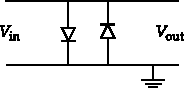
\includegraphics[scale=1.2]{report_img/diodes} 
		\caption{The double diode circuit is used to remove some of the amplitude of the signal before it is input to the mixer chip. This should allow a cleaner signal to be produced as the signal will be below the upper voltage limit of the chip.}
		\label{fig:diodes}
\end{figure} 

Another method to reduce the amplitude of the signal was attempted using a simple low pass filter. This time with a threshold frequency that is much higher than the wave which means that some of the frequencies that make up the square wave are removed. This will have the effect of reducing the overall amplitude of the wave, but at the expense of turning the square wave into a triangular wave. When implemented, this circuit had the desired effect of reducing the amplitude, but to such a degree that the signal is completely inaudible now. The amount of control over the properties of this circuit is limited and so this attempt is abandoned. 

\subsection{Quantitative Characteristics}
The nature of the variation of the produced signal with respect to the position of the user's hand is the product of several laws that govern separate components of the circuit. For example, the capacitance of the capacitor itself is inversely proportional to $d$ and the frequency of the oscillator chip is inversely proportional to $C$. This meant that the expect relation between the distance and the capacitance was
\begin{align}
	f &\propto \frac{1}{C} \propto \frac{1}{\frac{1}{d}} = d \nonumber \\
	\therefore f &\propto d 
\end{align}
This however was not seen when the frequency is measured with respect to the distance between the plates. When this was measured, shown in figure~\ref{fig:distance frequency}, the relation was found to be $f \propto \frac{1}{d}$.

\begin{figure}[ht]
	\centering
	\begin{minipage}[c]{0.3\textwidth}
		\begin{tabular}{r@{.}l|r@{.}l||r@{.}l|r@{.}l}
			\multicolumn{2}{c|}{\rotatebox{90}{Distance (cm)}} & \multicolumn{2}{c||}{\rotatebox{90}{Frequency (Hz)}} & \multicolumn{2}{c|}{\rotatebox{90}{Distance (cm)}} & \multicolumn{2}{c}{\rotatebox{90}{Frequency (Hz)}} \\ \hline \hline
			36&8	& 1&4 & 8&8	& 4&1 \\
			34&0	& 1&5 & 7&4	& 5&0 \\
			32&0	& 1&7 & 5&2	& 6&0 \\
			26&8	& 2&0 & 4&6	& 7&0 \\
			23&3	& 2&2 & 3&4	& 8&0 \\
			18&9	& 2&5 & 2&7	& 9&0 \\
			14&8	& 3&0 & 2&2	& 11&0 \\
			12&9	& 3&3 & 1&5	& 13&0 \\
			10&6	& 3&9 \\
		\end{tabular}
	\end{minipage}
	\begin{minipage}[c]{0.65\textwidth}
		\centering
		\centering
				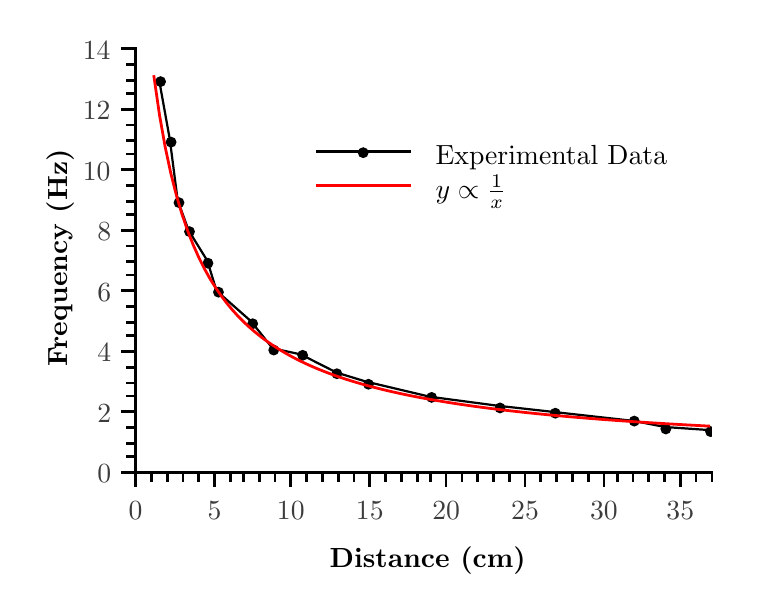
\begin{tikzpicture}{0pt}{0pt}{269pt}{209pt}
	\clip(0pt,209pt) -- (255.798pt,209pt) -- (255.798pt,10.2575pt) -- (0pt,10.2575pt) -- (0pt,209pt);
\begin{scope}
	\clip(38.9878pt,201.393pt) -- (247.239pt,201.393pt) -- (247.239pt,48.2943pt) -- (38.9878pt,48.2943pt) -- (38.9878pt,201.393pt);
	\color[rgb]{0,0,0}
	\draw[line width=0.8pt, line join=miter, line cap=rect](246.114pt,63.6042pt) -- (230.354pt,64.6977pt) -- (219.097pt,66.8848pt) -- (189.83pt,70.1655pt) -- (170.13pt,72.3526pt) -- (145.365pt,75.6333pt) -- (122.288pt,81.1011pt) -- (111.594pt,84.3818pt) -- (98.6491pt,90.9432pt) -- (88.5179pt,93.1303pt) -- (80.6381pt,102.972pt) -- (68.2556pt,113.908pt) -- (64.8785pt,124.843pt) -- (58.1244pt,135.779pt) -- (54.1845pt,146.715pt) -- (51.3703pt,168.586pt) -- (47.4304pt,190.457pt);
	\color[rgb]{0,0,0}
	\fill(246.764pt,63.0336pt) ellipse (1.42638pt and 1.42638pt);
	\draw[line width=1pt, line join=miter, line cap=rect](246.764pt,63.0336pt) ellipse (1.42638pt and 1.42638pt);
	\fill(230.598pt,63.9845pt) ellipse (1.42638pt and 1.42638pt);
	\draw[line width=1pt, line join=miter, line cap=rect](230.598pt,63.9845pt) ellipse (1.42638pt and 1.42638pt);
	\fill(219.187pt,66.8373pt) ellipse (1.42638pt and 1.42638pt);
	\draw[line width=1pt, line join=miter, line cap=rect](219.187pt,66.8373pt) ellipse (1.42638pt and 1.42638pt);
	\fill(190.66pt,69.6901pt) ellipse (1.42638pt and 1.42638pt);
	\draw[line width=1pt, line join=miter, line cap=rect](190.66pt,69.6901pt) ellipse (1.42638pt and 1.42638pt);
	\fill(170.69pt,71.5919pt) ellipse (1.42638pt and 1.42638pt);
	\draw[line width=1pt, line join=miter, line cap=rect](170.69pt,71.5919pt) ellipse (1.42638pt and 1.42638pt);
	\fill(145.966pt,75.3956pt) ellipse (1.42638pt and 1.42638pt);
	\draw[line width=1pt, line join=miter, line cap=rect](145.966pt,75.3956pt) ellipse (1.42638pt and 1.42638pt);
	\fill(123.144pt,80.1502pt) ellipse (1.42638pt and 1.42638pt);
	\draw[line width=1pt, line join=miter, line cap=rect](123.144pt,80.1502pt) ellipse (1.42638pt and 1.42638pt);
	\fill(111.733pt,83.9539pt) ellipse (1.42638pt and 1.42638pt);
	\draw[line width=1pt, line join=miter, line cap=rect](111.733pt,83.9539pt) ellipse (1.42638pt and 1.42638pt);
	\fill(99.3712pt,90.6103pt) ellipse (1.42638pt and 1.42638pt);
	\draw[line width=1pt, line join=miter, line cap=rect](99.3712pt,90.6103pt) ellipse (1.42638pt and 1.42638pt);
	\fill(88.9111pt,92.5122pt) ellipse (1.42638pt and 1.42638pt);
	\draw[line width=1pt, line join=miter, line cap=rect](88.9111pt,92.5122pt) ellipse (1.42638pt and 1.42638pt);
	\fill(81.3037pt,102.021pt) ellipse (1.42638pt and 1.42638pt);
	\draw[line width=1pt, line join=miter, line cap=rect](81.3037pt,102.021pt) ellipse (1.42638pt and 1.42638pt);
	\fill(68.9418pt,113.432pt) ellipse (1.42638pt and 1.42638pt);
	\draw[line width=1pt, line join=miter, line cap=rect](68.9418pt,113.432pt) ellipse (1.42638pt and 1.42638pt);
	\fill(65.1381pt,123.893pt) ellipse (1.42638pt and 1.42638pt);
	\draw[line width=1pt, line join=miter, line cap=rect](65.1381pt,123.893pt) ellipse (1.42638pt and 1.42638pt);
	\fill(58.4816pt,135.304pt) ellipse (1.42638pt and 1.42638pt);
	\draw[line width=1pt, line join=miter, line cap=rect](58.4816pt,135.304pt) ellipse (1.42638pt and 1.42638pt);
	\fill(54.678pt,145.764pt) ellipse (1.42638pt and 1.42638pt);
	\draw[line width=1pt, line join=miter, line cap=rect](54.678pt,145.764pt) ellipse (1.42638pt and 1.42638pt);
	\fill(51.8252pt,167.635pt) ellipse (1.42638pt and 1.42638pt);
	\draw[line width=1pt, line join=miter, line cap=rect](51.8252pt,167.635pt) ellipse (1.42638pt and 1.42638pt);
	\fill(48.0215pt,189.506pt) ellipse (1.42638pt and 1.42638pt);
	\draw[line width=1pt, line join=miter, line cap=rect](48.0215pt,189.506pt) ellipse (1.42638pt and 1.42638pt);
	\color[rgb]{1,0,0}
	\draw[line width=1pt, line join=bevel, line cap=rect](45.6293pt,191.317pt) -- (47.6544pt,177.335pt) -- (49.6795pt,165.934pt) -- (51.7046pt,156.458pt) -- (53.7297pt,148.459pt) -- (55.7548pt,141.616pt) -- (57.7799pt,135.695pt) -- (59.805pt,130.522pt) -- (61.8301pt,125.964pt) -- (63.8552pt,121.916pt) -- (65.8803pt,118.298pt) -- (67.9054pt,115.045pt) -- (69.9305pt,112.104pt) -- (71.9555pt,109.433pt) -- (73.9806pt,106.995pt) -- (76.0057pt,104.762pt) -- (78.0308pt,102.709pt) -- (80.0559pt,100.814pt) -- (82.081pt,99.0611pt) -- (84.1061pt,97.4339pt) -- (86.1312pt,95.9196pt) -- (88.1563pt,94.5067pt) -- (90.1814pt,93.1855pt) -- (92.2065pt,91.9472pt) -- (94.2316pt,90.7844pt) -- (96.2567pt,89.6903pt) -- (98.2818pt,88.659pt) -- (100.307pt,87.6853pt) -- (102.332pt,86.7644pt) -- (104.357pt,85.8922pt) -- (106.382pt,85.065pt) -- (108.407pt,84.2792pt) -- (110.432pt,83.5319pt) -- (112.457pt,82.8204pt) -- (114.483pt,82.1421pt) -- (116.508pt,81.4947pt) -- (118.533pt,80.8762pt) -- (120.558pt,80.2847pt) -- (122.583pt,79.7184pt) -- (124.608pt,79.1758pt) -- (126.633pt,78.6555pt) -- (128.658pt,78.156pt) -- (130.683pt,77.6762pt) -- (132.708pt,77.2148pt) -- (134.734pt,76.771pt) -- (136.759pt,76.3436pt) -- (138.784pt,75.9318pt) -- (140.809pt,75.5348pt) -- (142.834pt,75.1517pt) -- (144.859pt,74.7819pt) -- (146.884pt,74.4247pt) -- (148.909pt,74.0794pt) -- (150.934pt,73.7454pt) -- (152.959pt,73.4223pt) -- (154.984pt,73.1094pt) -- (157.01pt,72.8063pt) -- (159.035pt,72.5126pt) -- (161.06pt,72.2278pt) -- (163.085pt,71.9515pt) -- (165.11pt,71.6834pt) -- (167.135pt,71.4231pt) -- (169.16pt,71.1702pt) -- (171.185pt,70.9244pt) -- (173.21pt,70.6855pt) -- (175.235pt,70.4532pt) -- (177.261pt,70.2271pt) -- (179.286pt,70.0071pt) -- (181.311pt,69.7929pt) -- (183.336pt,69.5843pt) -- (185.361pt,69.381pt) -- (187.386pt,69.1829pt) -- (189.411pt,68.9898pt) -- (191.436pt,68.8014pt) -- (193.461pt,68.6176pt) -- (195.486pt,68.4383pt) -- (197.511pt,68.2632pt) -- (199.537pt,68.0923pt) -- (201.562pt,67.9254pt) -- (203.587pt,67.7623pt) -- (205.612pt,67.6029pt) -- (207.637pt,67.4471pt) -- (209.662pt,67.2948pt) -- (211.687pt,67.1458pt) -- (213.712pt,67.0001pt) -- (215.737pt,66.8575pt) -- (217.762pt,66.7179pt) -- (219.788pt,66.5813pt) -- (221.813pt,66.4475pt) -- (223.838pt,66.3166pt) -- (225.863pt,66.1882pt) -- (227.888pt,66.0625pt) -- (229.913pt,65.9393pt) -- (231.938pt,65.8186pt) -- (233.963pt,65.7002pt) -- (235.988pt,65.5841pt) -- (238.013pt,65.4702pt) -- (240.039pt,65.3586pt) -- (242.064pt,65.249pt) -- (244.089pt,65.1415pt) -- (246.114pt,65.0359pt);
\end{scope}
\begin{scope}
	\color[rgb]{0,0,0}
	\pgftext[center, base, at={\pgfpoint{14.2638pt}{125.794pt}},rotate=90]{\textbf{Frequency (Hz)}}
	\color[rgb]{0.235294,0.235294,0.235294}
	\pgftext[center, base, at={\pgfpoint{27.6881pt}{44.4907pt}}]{0}
	\pgftext[center, base, at={\pgfpoint{27.6881pt}{66.3618pt}}]{2}
	\pgftext[center, base, at={\pgfpoint{27.6881pt}{88.233pt}}]{4}
	\pgftext[center, base, at={\pgfpoint{27.6881pt}{110.104pt}}]{6}
	\pgftext[center, base, at={\pgfpoint{27.6881pt}{131.975pt}}]{8}
	\pgftext[center, base, at={\pgfpoint{24.9468pt}{153.847pt}}]{10}
	\pgftext[center, base, at={\pgfpoint{24.9468pt}{175.718pt}}]{12}
	\pgftext[center, base, at={\pgfpoint{24.9468pt}{197.589pt}}]{14}
	\color[rgb]{0,0,0}
	\draw[line width=1pt, line join=bevel, line cap=rect](38.9878pt,53.9999pt) -- (36.135pt,53.9999pt);
	\draw[line width=1pt, line join=bevel, line cap=rect](38.9878pt,64.46pt) -- (36.135pt,64.46pt);
	\draw[line width=1pt, line join=bevel, line cap=rect](38.9878pt,75.8711pt) -- (36.135pt,75.8711pt);
	\draw[line width=1pt, line join=bevel, line cap=rect](38.9878pt,86.3312pt) -- (36.135pt,86.3312pt);
	\draw[line width=1pt, line join=bevel, line cap=rect](38.9878pt,97.7422pt) -- (36.135pt,97.7422pt);
	\draw[line width=1pt, line join=bevel, line cap=rect](38.9878pt,108.202pt) -- (36.135pt,108.202pt);
	\draw[line width=1pt, line join=bevel, line cap=rect](38.9878pt,119.613pt) -- (36.135pt,119.613pt);
	\draw[line width=1pt, line join=bevel, line cap=rect](38.9878pt,130.074pt) -- (36.135pt,130.074pt);
	\draw[line width=1pt, line join=bevel, line cap=rect](38.9878pt,141.485pt) -- (36.135pt,141.485pt);
	\draw[line width=1pt, line join=bevel, line cap=rect](38.9878pt,151.945pt) -- (36.135pt,151.945pt);
	\draw[line width=1pt, line join=bevel, line cap=rect](38.9878pt,163.356pt) -- (36.135pt,163.356pt);
	\draw[line width=1pt, line join=bevel, line cap=rect](38.9878pt,173.816pt) -- (36.135pt,173.816pt);
	\draw[line width=1pt, line join=bevel, line cap=rect](38.9878pt,185.227pt) -- (36.135pt,185.227pt);
	\draw[line width=1pt, line join=bevel, line cap=rect](38.9878pt,195.687pt) -- (36.135pt,195.687pt);
	\draw[line width=1pt, line join=bevel, line cap=rect](38.9878pt,58.7545pt) -- (36.135pt,58.7545pt);
	\draw[line width=1pt, line join=bevel, line cap=rect](38.9878pt,80.6257pt) -- (36.135pt,80.6257pt);
	\draw[line width=1pt, line join=bevel, line cap=rect](38.9878pt,102.497pt) -- (36.135pt,102.497pt);
	\draw[line width=1pt, line join=bevel, line cap=rect](38.9878pt,124.368pt) -- (36.135pt,124.368pt);
	\draw[line width=1pt, line join=bevel, line cap=rect](38.9878pt,146.239pt) -- (36.135pt,146.239pt);
	\draw[line width=1pt, line join=bevel, line cap=rect](38.9878pt,168.11pt) -- (36.135pt,168.11pt);
	\draw[line width=1pt, line join=bevel, line cap=rect](38.9878pt,189.982pt) -- (36.135pt,189.982pt);
	\draw[line width=1pt, line join=bevel, line cap=rect](38.9878pt,48.2943pt) -- (34.2332pt,48.2943pt);
	\draw[line width=1pt, line join=bevel, line cap=rect](38.9878pt,70.1655pt) -- (34.2332pt,70.1655pt);
	\draw[line width=1pt, line join=bevel, line cap=rect](38.9878pt,92.0367pt) -- (34.2332pt,92.0367pt);
	\draw[line width=1pt, line join=bevel, line cap=rect](38.9878pt,113.908pt) -- (34.2332pt,113.908pt);
	\draw[line width=1pt, line join=bevel, line cap=rect](38.9878pt,135.779pt) -- (34.2332pt,135.779pt);
	\draw[line width=1pt, line join=bevel, line cap=rect](38.9878pt,157.65pt) -- (34.2332pt,157.65pt);
	\draw[line width=1pt, line join=bevel, line cap=rect](38.9878pt,179.521pt) -- (34.2332pt,179.521pt);
	\draw[line width=1pt, line join=bevel, line cap=rect](38.9878pt,201.393pt) -- (34.2332pt,201.393pt);
	\draw[line width=1pt, line join=bevel, line cap=rect](38.9878pt,201.393pt) -- (38.9878pt,48.2943pt);
	\pgftext[center, base, at={\pgfpoint{144.533pt}{14.0612pt}}]{\textbf{Distance (cm)}}
	\color[rgb]{0.235294,0.235294,0.235294}
	\pgftext[center, base, at={\pgfpoint{38.9803pt}{31.1778pt}}]{0}
	\pgftext[center, base, at={\pgfpoint{67.508pt}{31.1778pt}}]{5}
	\pgftext[center, base, at={\pgfpoint{95.0921pt}{31.1778pt}}]{10}
	\pgftext[center, base, at={\pgfpoint{123.62pt}{31.1778pt}}]{15}
	\pgftext[center, base, at={\pgfpoint{151.196pt}{31.1778pt}}]{20}
	\pgftext[center, base, at={\pgfpoint{179.724pt}{31.1778pt}}]{25}
	\pgftext[center, base, at={\pgfpoint{208.252pt}{31.1778pt}}]{30}
	\pgftext[center, base, at={\pgfpoint{235.828pt}{31.1778pt}}]{35}
	\color[rgb]{0,0,0}
	\draw[line width=1pt, line join=bevel, line cap=rect](44.6933pt,48.2943pt) -- (44.6933pt,45.4416pt);
	\draw[line width=1pt, line join=bevel, line cap=rect](50.3988pt,48.2943pt) -- (50.3988pt,45.4416pt);
	\draw[line width=1pt, line join=bevel, line cap=rect](56.1043pt,48.2943pt) -- (56.1043pt,45.4416pt);
	\draw[line width=1pt, line join=bevel, line cap=rect](61.8099pt,48.2943pt) -- (61.8099pt,45.4416pt);
	\draw[line width=1pt, line join=bevel, line cap=rect](73.2209pt,48.2943pt) -- (73.2209pt,45.4416pt);
	\draw[line width=1pt, line join=bevel, line cap=rect](77.9755pt,48.2943pt) -- (77.9755pt,45.4416pt);
	\draw[line width=1pt, line join=bevel, line cap=rect](83.6811pt,48.2943pt) -- (83.6811pt,45.4416pt);
	\draw[line width=1pt, line join=bevel, line cap=rect](89.3866pt,48.2943pt) -- (89.3866pt,45.4416pt);
	\draw[line width=1pt, line join=bevel, line cap=rect](100.798pt,48.2943pt) -- (100.798pt,45.4416pt);
	\draw[line width=1pt, line join=bevel, line cap=rect](106.503pt,48.2943pt) -- (106.503pt,45.4416pt);
	\draw[line width=1pt, line join=bevel, line cap=rect](112.209pt,48.2943pt) -- (112.209pt,45.4416pt);
	\draw[line width=1pt, line join=bevel, line cap=rect](117.914pt,48.2943pt) -- (117.914pt,45.4416pt);
	\draw[line width=1pt, line join=bevel, line cap=rect](129.325pt,48.2943pt) -- (129.325pt,45.4416pt);
	\draw[line width=1pt, line join=bevel, line cap=rect](135.031pt,48.2943pt) -- (135.031pt,45.4416pt);
	\draw[line width=1pt, line join=bevel, line cap=rect](140.736pt,48.2943pt) -- (140.736pt,45.4416pt);
	\draw[line width=1pt, line join=bevel, line cap=rect](145.491pt,48.2943pt) -- (145.491pt,45.4416pt);
	\draw[line width=1pt, line join=bevel, line cap=rect](156.902pt,48.2943pt) -- (156.902pt,45.4416pt);
	\draw[line width=1pt, line join=bevel, line cap=rect](162.607pt,48.2943pt) -- (162.607pt,45.4416pt);
	\draw[line width=1pt, line join=bevel, line cap=rect](168.313pt,48.2943pt) -- (168.313pt,45.4416pt);
	\draw[line width=1pt, line join=bevel, line cap=rect](174.019pt,48.2943pt) -- (174.019pt,45.4416pt);
	\draw[line width=1pt, line join=bevel, line cap=rect](185.43pt,48.2943pt) -- (185.43pt,45.4416pt);
	\draw[line width=1pt, line join=bevel, line cap=rect](191.135pt,48.2943pt) -- (191.135pt,45.4416pt);
	\draw[line width=1pt, line join=bevel, line cap=rect](196.841pt,48.2943pt) -- (196.841pt,45.4416pt);
	\draw[line width=1pt, line join=bevel, line cap=rect](202.546pt,48.2943pt) -- (202.546pt,45.4416pt);
	\draw[line width=1pt, line join=bevel, line cap=rect](213.006pt,48.2943pt) -- (213.006pt,45.4416pt);
	\draw[line width=1pt, line join=bevel, line cap=rect](218.712pt,48.2943pt) -- (218.712pt,45.4416pt);
	\draw[line width=1pt, line join=bevel, line cap=rect](224.417pt,48.2943pt) -- (224.417pt,45.4416pt);
	\draw[line width=1pt, line join=bevel, line cap=rect](230.123pt,48.2943pt) -- (230.123pt,45.4416pt);
	\draw[line width=1pt, line join=bevel, line cap=rect](241.534pt,48.2943pt) -- (241.534pt,45.4416pt);
	\draw[line width=1pt, line join=bevel, line cap=rect](247.239pt,48.2943pt) -- (247.239pt,45.4416pt);
	\draw[line width=1pt, line join=bevel, line cap=rect](38.9878pt,48.2943pt) -- (38.9878pt,43.5397pt);
	\draw[line width=1pt, line join=bevel, line cap=rect](67.5154pt,48.2943pt) -- (67.5154pt,43.5397pt);
	\draw[line width=1pt, line join=bevel, line cap=rect](95.0921pt,48.2943pt) -- (95.0921pt,43.5397pt);
	\draw[line width=1pt, line join=bevel, line cap=rect](123.62pt,48.2943pt) -- (123.62pt,43.5397pt);
	\draw[line width=1pt, line join=bevel, line cap=rect](151.196pt,48.2943pt) -- (151.196pt,43.5397pt);
	\draw[line width=1pt, line join=bevel, line cap=rect](179.724pt,48.2943pt) -- (179.724pt,43.5397pt);
	\draw[line width=1pt, line join=bevel, line cap=rect](208.252pt,48.2943pt) -- (208.252pt,43.5397pt);
	\draw[line width=1pt, line join=bevel, line cap=rect](235.828pt,48.2943pt) -- (235.828pt,43.5397pt);
	\draw[line width=1pt, line join=bevel, line cap=rect](38.9878pt,48.2943pt) -- (247.239pt,48.2943pt);
	\draw[line width=1pt, line join=miter, line cap=rect](104.601pt,164.307pt) -- (137.884pt,164.307pt);
	\fill(121.242pt,163.831pt) ellipse (1.42638pt and 1.42638pt);
	\draw[line width=1pt, line join=miter, line cap=rect](121.242pt,163.831pt) ellipse (1.42638pt and 1.42638pt);
	\pgftext[left, base, at={\pgfpoint{147.393pt}{159.552pt}}]{Experimental Data}
	\color[rgb]{1,0,0}
	\draw[line width=1pt, line join=bevel, line cap=rect](104.601pt,151.945pt) -- (137.884pt,151.945pt);
	\color[rgb]{0,0,0}
	\pgftext[left, base, at={\pgfpoint{147.393pt}{147.19pt}}]{$y \propto \frac{1}{x}$}
\end{scope}
\end{tikzpicture}
 
			\vspace{-10pt}
	\end{minipage}
	\caption{The distance from the plate capacitor against the frequency that this position produces is recorded.}
	\label{fig:distance frequency}
\end{figure}

Also, the action of the mixer chip was verified by measuring the output frequency produced when using a single VCO at a fixed frequency of 1.5\,MHz and the variable TG315 signal generator. This is shown in figure~\ref{fig:frequency generator}. The linear direct relationship can be clearly seen here. This graph is of the form $y=|x-c|$ where $c$ is a constant, since the two regions have the same slope. This confirms that the action of the mixer is as expected.  

\begin{figure}
	\begin{center}
		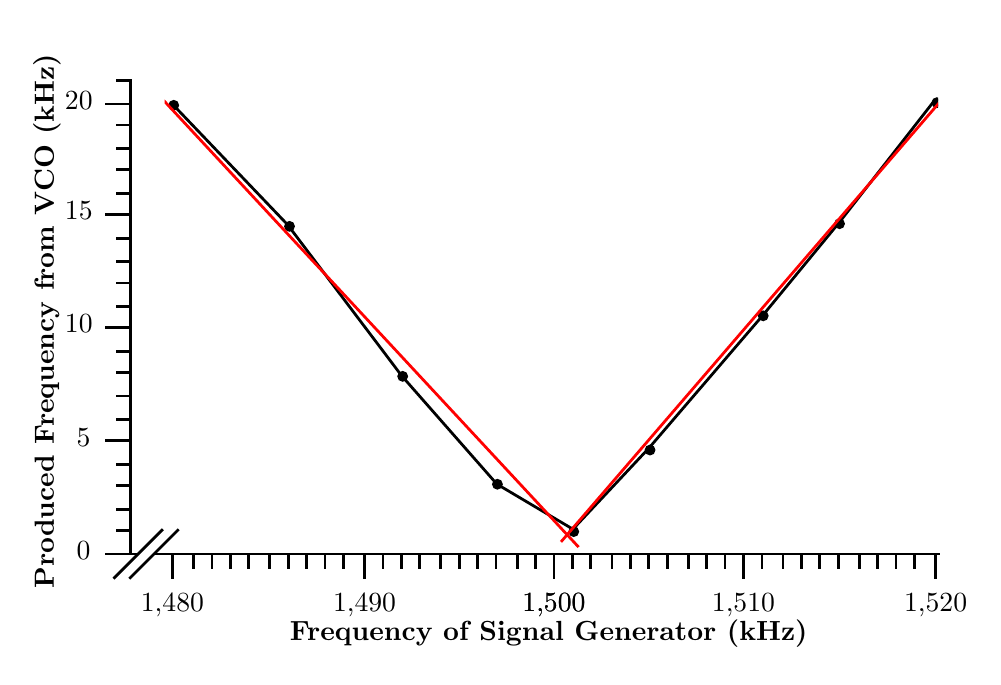
\begin{tikzpicture}{0pt}{0pt}{359pt}{239pt}
	\clip(0pt,239pt) -- (341.381pt,239pt) -- (341.381pt,11.7299pt) -- (0pt,11.7299pt) -- (0pt,239pt);
\begin{scope}
	\clip(49.4479pt,219.982pt) -- (329.019pt,219.982pt) -- (329.019pt,48.8158pt) -- (49.4479pt,48.8158pt) -- (49.4479pt,219.982pt);
	\color[rgb]{0,0,0}
	\draw[line width=1pt, line join=miter, line cap=rect](52.6521pt,211.016pt) -- (93.9009pt,167.817pt) -- (135.15pt,113.207pt) -- (169.524pt,74.0831pt) -- (197.023pt,57.7816pt) -- (224.522pt,87.1243pt) -- (265.771pt,135.214pt) -- (293.27pt,168.632pt) -- (327.644pt,212.646pt);
	\color[rgb]{0,0,0}
	\fill(52.7761pt,210.948pt) ellipse (1.42638pt and 1.42638pt);
	\draw[line width=1pt, line join=miter, line cap=rect](52.7761pt,210.948pt) ellipse (1.42638pt and 1.42638pt);
	\fill(94.6166pt,167.205pt) ellipse (1.42638pt and 1.42638pt);
	\draw[line width=1pt, line join=miter, line cap=rect](94.6166pt,167.205pt) ellipse (1.42638pt and 1.42638pt);
	\fill(135.506pt,113.003pt) ellipse (1.42638pt and 1.42638pt);
	\draw[line width=1pt, line join=miter, line cap=rect](135.506pt,113.003pt) ellipse (1.42638pt and 1.42638pt);
	\fill(169.739pt,74.0152pt) ellipse (1.42638pt and 1.42638pt);
	\draw[line width=1pt, line join=miter, line cap=rect](169.739pt,74.0152pt) ellipse (1.42638pt and 1.42638pt);
	\fill(197.316pt,56.8986pt) ellipse (1.42638pt and 1.42638pt);
	\draw[line width=1pt, line join=miter, line cap=rect](197.316pt,56.8986pt) ellipse (1.42638pt and 1.42638pt);
	\fill(224.893pt,86.3772pt) ellipse (1.42638pt and 1.42638pt);
	\draw[line width=1pt, line join=miter, line cap=rect](224.893pt,86.3772pt) ellipse (1.42638pt and 1.42638pt);
	\fill(265.782pt,134.874pt) ellipse (1.42638pt and 1.42638pt);
	\draw[line width=1pt, line join=miter, line cap=rect](265.782pt,134.874pt) ellipse (1.42638pt and 1.42638pt);
	\fill(293.359pt,168.156pt) ellipse (1.42638pt and 1.42638pt);
	\draw[line width=1pt, line join=miter, line cap=rect](293.359pt,168.156pt) ellipse (1.42638pt and 1.42638pt);
	\fill(328.543pt,211.899pt) ellipse (1.42638pt and 1.42638pt);
	\draw[line width=1pt, line join=miter, line cap=rect](328.543pt,211.899pt) ellipse (1.42638pt and 1.42638pt);
	\color[rgb]{1,0,0}
	\draw[line width=1pt, line join=miter, line cap=rect](334.724pt,218.08pt) -- (193.037pt,53.5704pt);
	\draw[line width=1pt, line join=miter, line cap=rect](49.4479pt,212.374pt) -- (198.742pt,51.6686pt);
\end{scope}
\begin{scope}
	\color[rgb]{0,0,0}
	\pgftext[center, base, at={\pgfpoint{188.275pt}{227.589pt}}]{\textbf{ }}
	\color[rgb]{0,0,0}
	\pgftext[center, base, at={\pgfpoint{9.50921pt}{132.972pt}},rotate=90]{\textbf{Produced Frequency from VCO (kHz)}}
	\pgftext[center, base, at={\pgfpoint{20.1774pt}{46.9139pt}}]{0}
	\pgftext[center, base, at={\pgfpoint{20.1774pt}{87.8036pt}}]{5}
	\pgftext[center, base, at={\pgfpoint{18.4835pt}{128.693pt}}]{10}
	\pgftext[center, base, at={\pgfpoint{18.4835pt}{169.583pt}}]{15}
	\pgftext[center, base, at={\pgfpoint{18.4835pt}{209.521pt}}]{20}
	\draw[line width=1pt, line join=bevel, line cap=rect](37.0859pt,57.3741pt) -- (32.3313pt,57.3741pt);
	\draw[line width=1pt, line join=bevel, line cap=rect](37.0859pt,64.9814pt) -- (32.3313pt,64.9814pt);
	\draw[line width=1pt, line join=bevel, line cap=rect](37.0859pt,73.5397pt) -- (32.3313pt,73.5397pt);
	\draw[line width=1pt, line join=bevel, line cap=rect](37.0859pt,81.1471pt) -- (32.3313pt,81.1471pt);
	\draw[line width=1pt, line join=bevel, line cap=rect](37.0859pt,97.3128pt) -- (32.3313pt,97.3128pt);
	\draw[line width=1pt, line join=bevel, line cap=rect](37.0859pt,105.871pt) -- (32.3313pt,105.871pt);
	\draw[line width=1pt, line join=bevel, line cap=rect](37.0859pt,114.429pt) -- (32.3313pt,114.429pt);
	\draw[line width=1pt, line join=bevel, line cap=rect](37.0859pt,122.037pt) -- (32.3313pt,122.037pt);
	\draw[line width=1pt, line join=bevel, line cap=rect](37.0859pt,138.202pt) -- (32.3313pt,138.202pt);
	\draw[line width=1pt, line join=bevel, line cap=rect](37.0859pt,146.761pt) -- (32.3313pt,146.761pt);
	\draw[line width=1pt, line join=bevel, line cap=rect](37.0859pt,154.368pt) -- (32.3313pt,154.368pt);
	\draw[line width=1pt, line join=bevel, line cap=rect](37.0859pt,162.926pt) -- (32.3313pt,162.926pt);
	\draw[line width=1pt, line join=bevel, line cap=rect](37.0859pt,179.092pt) -- (32.3313pt,179.092pt);
	\draw[line width=1pt, line join=bevel, line cap=rect](37.0859pt,187.65pt) -- (32.3313pt,187.65pt);
	\draw[line width=1pt, line join=bevel, line cap=rect](37.0859pt,195.258pt) -- (32.3313pt,195.258pt);
	\draw[line width=1pt, line join=bevel, line cap=rect](37.0859pt,203.816pt) -- (32.3313pt,203.816pt);
	\draw[line width=1pt, line join=bevel, line cap=rect](37.0859pt,219.982pt) -- (32.3313pt,219.982pt);
	\draw[line width=1pt, line join=bevel, line cap=rect](37.0859pt,48.8158pt) -- (28.5276pt,48.8158pt);
	\draw[line width=1pt, line join=bevel, line cap=rect](37.0859pt,89.7054pt) -- (28.5276pt,89.7054pt);
	\draw[line width=1pt, line join=bevel, line cap=rect](37.0859pt,130.595pt) -- (28.5276pt,130.595pt);
	\draw[line width=1pt, line join=bevel, line cap=rect](37.0859pt,171.485pt) -- (28.5276pt,171.485pt);
	\draw[line width=1pt, line join=bevel, line cap=rect](37.0859pt,211.423pt) -- (28.5276pt,211.423pt);
	\draw[line width=1pt, line join=bevel, line cap=rect](37.0859pt,219.982pt) -- (37.0859pt,48.8158pt);
	\pgftext[center, base, at={\pgfpoint{188.275pt}{17.4354pt}}]{\textbf{Frequency of Signal Generator (kHz)}}
	\draw[line width=1pt, line join=bevel, line cap=rect](48.497pt,57.3741pt) -- (31.3804pt,40.2575pt);
	\draw[line width=1pt, line join=bevel, line cap=rect](54.2025pt,57.3741pt) -- (37.0859pt,40.2575pt);
	\pgftext[center, base, at={\pgfpoint{190.184pt}{27.8955pt}}]{1,500}
	\pgftext[center, base, at={\pgfpoint{52.3007pt}{27.8955pt}}]{1,480}
	\pgftext[center, base, at={\pgfpoint{121.718pt}{27.8955pt}}]{1,490}
	\pgftext[center, base, at={\pgfpoint{190.184pt}{27.8955pt}}]{1,500}
	\pgftext[center, base, at={\pgfpoint{258.651pt}{27.8955pt}}]{1,510}
	\pgftext[center, base, at={\pgfpoint{328.068pt}{27.8955pt}}]{1,520}
	\draw[line width=1pt, line join=bevel, line cap=rect](59.908pt,48.8158pt) -- (59.908pt,44.0612pt);
	\draw[line width=1pt, line join=bevel, line cap=rect](66.5645pt,48.8158pt) -- (66.5645pt,44.0612pt);
	\draw[line width=1pt, line join=bevel, line cap=rect](73.2209pt,48.8158pt) -- (73.2209pt,44.0612pt);
	\draw[line width=1pt, line join=bevel, line cap=rect](79.8774pt,48.8158pt) -- (79.8774pt,44.0612pt);
	\draw[line width=1pt, line join=bevel, line cap=rect](94.1412pt,48.8158pt) -- (94.1412pt,44.0612pt);
	\draw[line width=1pt, line join=bevel, line cap=rect](100.798pt,48.8158pt) -- (100.798pt,44.0612pt);
	\draw[line width=1pt, line join=bevel, line cap=rect](107.454pt,48.8158pt) -- (107.454pt,44.0612pt);
	\draw[line width=1pt, line join=bevel, line cap=rect](114.111pt,48.8158pt) -- (114.111pt,44.0612pt);
	\draw[line width=1pt, line join=bevel, line cap=rect](128.374pt,48.8158pt) -- (128.374pt,44.0612pt);
	\draw[line width=1pt, line join=bevel, line cap=rect](135.031pt,48.8158pt) -- (135.031pt,44.0612pt);
	\draw[line width=1pt, line join=bevel, line cap=rect](141.687pt,48.8158pt) -- (141.687pt,44.0612pt);
	\draw[line width=1pt, line join=bevel, line cap=rect](149.295pt,48.8158pt) -- (149.295pt,44.0612pt);
	\draw[line width=1pt, line join=bevel, line cap=rect](162.607pt,48.8158pt) -- (162.607pt,44.0612pt);
	\draw[line width=1pt, line join=bevel, line cap=rect](169.264pt,48.8158pt) -- (169.264pt,44.0612pt);
	\draw[line width=1pt, line join=bevel, line cap=rect](176.871pt,48.8158pt) -- (176.871pt,44.0612pt);
	\draw[line width=1pt, line join=bevel, line cap=rect](183.528pt,48.8158pt) -- (183.528pt,44.0612pt);
	\draw[line width=1pt, line join=bevel, line cap=rect](196.841pt,48.8158pt) -- (196.841pt,44.0612pt);
	\draw[line width=1pt, line join=bevel, line cap=rect](203.497pt,48.8158pt) -- (203.497pt,44.0612pt);
	\draw[line width=1pt, line join=bevel, line cap=rect](211.104pt,48.8158pt) -- (211.104pt,44.0612pt);
	\draw[line width=1pt, line join=bevel, line cap=rect](217.761pt,48.8158pt) -- (217.761pt,44.0612pt);
	\draw[line width=1pt, line join=bevel, line cap=rect](231.074pt,48.8158pt) -- (231.074pt,44.0612pt);
	\draw[line width=1pt, line join=bevel, line cap=rect](238.681pt,48.8158pt) -- (238.681pt,44.0612pt);
	\draw[line width=1pt, line join=bevel, line cap=rect](245.338pt,48.8158pt) -- (245.338pt,44.0612pt);
	\draw[line width=1pt, line join=bevel, line cap=rect](251.994pt,48.8158pt) -- (251.994pt,44.0612pt);
	\draw[line width=1pt, line join=bevel, line cap=rect](265.307pt,48.8158pt) -- (265.307pt,44.0612pt);
	\draw[line width=1pt, line join=bevel, line cap=rect](272.914pt,48.8158pt) -- (272.914pt,44.0612pt);
	\draw[line width=1pt, line join=bevel, line cap=rect](279.571pt,48.8158pt) -- (279.571pt,44.0612pt);
	\draw[line width=1pt, line join=bevel, line cap=rect](286.227pt,48.8158pt) -- (286.227pt,44.0612pt);
	\draw[line width=1pt, line join=bevel, line cap=rect](300.491pt,48.8158pt) -- (300.491pt,44.0612pt);
	\draw[line width=1pt, line join=bevel, line cap=rect](307.147pt,48.8158pt) -- (307.147pt,44.0612pt);
	\draw[line width=1pt, line join=bevel, line cap=rect](313.804pt,48.8158pt) -- (313.804pt,44.0612pt);
	\draw[line width=1pt, line join=bevel, line cap=rect](320.46pt,48.8158pt) -- (320.46pt,44.0612pt);
	\draw[line width=1pt, line join=bevel, line cap=rect](87.4847pt,48.8158pt) -- (87.4847pt,44.0612pt);
	\draw[line width=1pt, line join=bevel, line cap=rect](155.951pt,48.8158pt) -- (155.951pt,44.0612pt);
	\draw[line width=1pt, line join=bevel, line cap=rect](224.417pt,48.8158pt) -- (224.417pt,44.0612pt);
	\draw[line width=1pt, line join=bevel, line cap=rect](292.884pt,48.8158pt) -- (292.884pt,44.0612pt);
	\draw[line width=1pt, line join=bevel, line cap=rect](190.184pt,48.8158pt) -- (190.184pt,40.2575pt);
	\draw[line width=1pt, line join=bevel, line cap=rect](52.3007pt,48.8158pt) -- (52.3007pt,40.2575pt);
	\draw[line width=1pt, line join=bevel, line cap=rect](121.718pt,48.8158pt) -- (121.718pt,40.2575pt);
	\draw[line width=1pt, line join=bevel, line cap=rect](190.184pt,48.8158pt) -- (190.184pt,40.2575pt);
	\draw[line width=1pt, line join=bevel, line cap=rect](258.651pt,48.8158pt) -- (258.651pt,40.2575pt);
	\draw[line width=1pt, line join=bevel, line cap=rect](328.068pt,48.8158pt) -- (328.068pt,40.2575pt);
	\draw[line width=1pt, line join=bevel, line cap=rect](37.0859pt,48.8158pt) -- (38.9878pt,48.8158pt);
	\draw[line width=1pt, line join=bevel, line cap=rect](46.5951pt,48.8158pt) -- (329.019pt,48.8158pt);
\end{scope}
\end{tikzpicture}

		\caption{As the generator input frequency to the mixer is increased, the difference between the generator and the reference VCO decreases, and so does the output frequency produced, until the generator is greater than the reference and so the difference, and so the output frequency, increases.}
		\label{fig:frequency generator}
	\end{center}
\end{figure}

Finally the relationship between the frequency of the input to the low pass circuit and the peak to peak voltage of the output of low pass circuit was measured. This allowed the characteristics of the signal with respect to the voltage to be observed. As can be seen in figure~\ref{fig:bode}, this is essentially a Bode plot with a cut off frequency of around 23.5\,kHz, just above human hearing range. This confirmed what was expected. As the frequency increases, the voltage is almost constant, up until the cut off frequency where the voltage is attenuated swiftly. This is due to the effect of the low pass filter removing the high frequency signals as desired.

\begin{figure}
	\begin{center}
		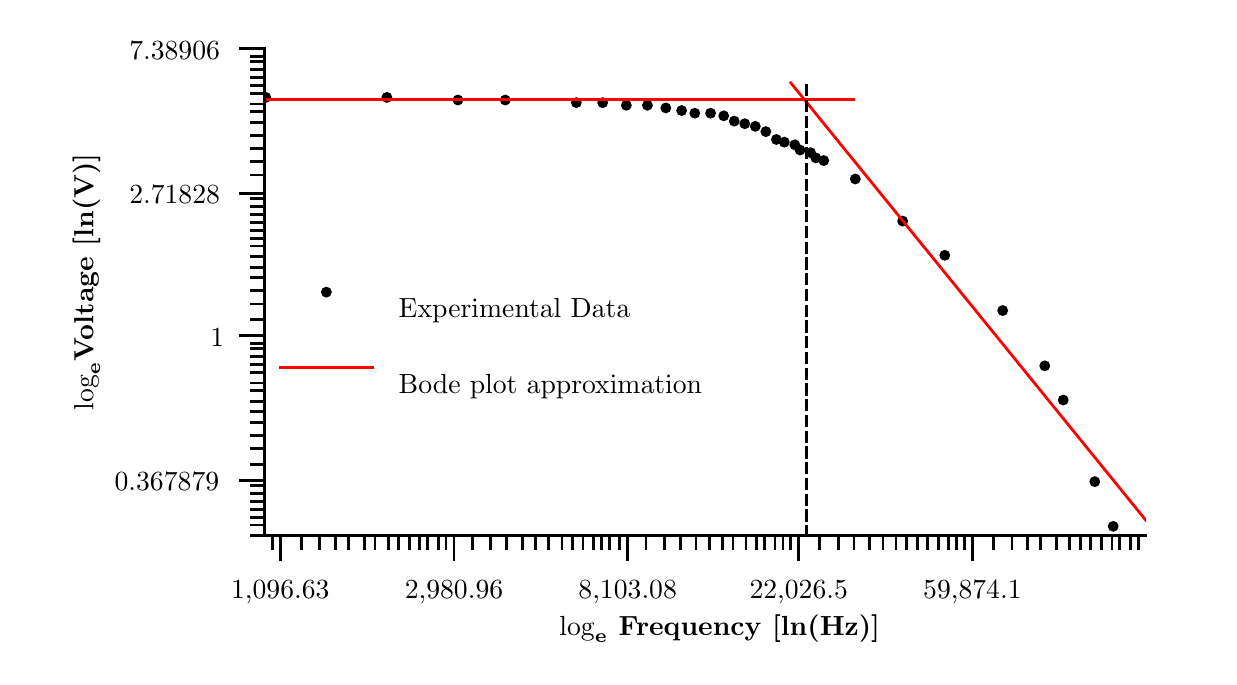
\begin{tikzpicture}{0pt}{0pt}{449pt}{239pt}
	\clip(0pt,239pt) -- (426.964pt,239pt) -- (426.964pt,11.7299pt) -- (0pt,11.7299pt) -- (0pt,239pt);
\begin{scope}
	\clip(85.5829pt,231.393pt) -- (404.141pt,231.393pt) -- (404.141pt,55.4722pt) -- (85.5829pt,55.4722pt) -- (85.5829pt,231.393pt);
	\color[rgb]{0,0,0}
	\fill(86.0584pt,213.801pt) ellipse (1.42638pt and 1.42638pt);
	\draw[line width=1pt, line join=miter, line cap=rect](86.0584pt,213.801pt) ellipse (1.42638pt and 1.42638pt);
	\color[rgb]{0,0,0}
	\fill(129.801pt,213.801pt) ellipse (1.42638pt and 1.42638pt);
	\draw[line width=1pt, line join=miter, line cap=rect](129.801pt,213.801pt) ellipse (1.42638pt and 1.42638pt);
	\fill(155.476pt,212.85pt) ellipse (1.42638pt and 1.42638pt);
	\draw[line width=1pt, line join=miter, line cap=rect](155.476pt,212.85pt) ellipse (1.42638pt and 1.42638pt);
	\fill(172.592pt,212.85pt) ellipse (1.42638pt and 1.42638pt);
	\draw[line width=1pt, line join=miter, line cap=rect](172.592pt,212.85pt) ellipse (1.42638pt and 1.42638pt);
	\fill(198.267pt,211.899pt) ellipse (1.42638pt and 1.42638pt);
	\draw[line width=1pt, line join=miter, line cap=rect](198.267pt,211.899pt) ellipse (1.42638pt and 1.42638pt);
	\fill(207.776pt,211.899pt) ellipse (1.42638pt and 1.42638pt);
	\draw[line width=1pt, line join=miter, line cap=rect](207.776pt,211.899pt) ellipse (1.42638pt and 1.42638pt);
	\fill(216.335pt,210.948pt) ellipse (1.42638pt and 1.42638pt);
	\draw[line width=1pt, line join=miter, line cap=rect](216.335pt,210.948pt) ellipse (1.42638pt and 1.42638pt);
	\fill(223.942pt,210.948pt) ellipse (1.42638pt and 1.42638pt);
	\draw[line width=1pt, line join=miter, line cap=rect](223.942pt,210.948pt) ellipse (1.42638pt and 1.42638pt);
	\fill(230.598pt,209.997pt) ellipse (1.42638pt and 1.42638pt);
	\draw[line width=1pt, line join=miter, line cap=rect](230.598pt,209.997pt) ellipse (1.42638pt and 1.42638pt);
	\fill(236.304pt,209.046pt) ellipse (1.42638pt and 1.42638pt);
	\draw[line width=1pt, line join=miter, line cap=rect](236.304pt,209.046pt) ellipse (1.42638pt and 1.42638pt);
	\fill(241.058pt,208.095pt) ellipse (1.42638pt and 1.42638pt);
	\draw[line width=1pt, line join=miter, line cap=rect](241.058pt,208.095pt) ellipse (1.42638pt and 1.42638pt);
	\fill(246.764pt,208.095pt) ellipse (1.42638pt and 1.42638pt);
	\draw[line width=1pt, line join=miter, line cap=rect](246.764pt,208.095pt) ellipse (1.42638pt and 1.42638pt);
	\fill(251.519pt,207.144pt) ellipse (1.42638pt and 1.42638pt);
	\draw[line width=1pt, line join=miter, line cap=rect](251.519pt,207.144pt) ellipse (1.42638pt and 1.42638pt);
	\fill(255.322pt,205.242pt) ellipse (1.42638pt and 1.42638pt);
	\draw[line width=1pt, line join=miter, line cap=rect](255.322pt,205.242pt) ellipse (1.42638pt and 1.42638pt);
	\fill(259.126pt,204.291pt) ellipse (1.42638pt and 1.42638pt);
	\draw[line width=1pt, line join=miter, line cap=rect](259.126pt,204.291pt) ellipse (1.42638pt and 1.42638pt);
	\fill(262.93pt,203.34pt) ellipse (1.42638pt and 1.42638pt);
	\draw[line width=1pt, line join=miter, line cap=rect](262.93pt,203.34pt) ellipse (1.42638pt and 1.42638pt);
	\fill(266.733pt,201.439pt) ellipse (1.42638pt and 1.42638pt);
	\draw[line width=1pt, line join=miter, line cap=rect](266.733pt,201.439pt) ellipse (1.42638pt and 1.42638pt);
	\fill(270.537pt,198.586pt) ellipse (1.42638pt and 1.42638pt);
	\draw[line width=1pt, line join=miter, line cap=rect](270.537pt,198.586pt) ellipse (1.42638pt and 1.42638pt);
	\fill(273.39pt,197.635pt) ellipse (1.42638pt and 1.42638pt);
	\draw[line width=1pt, line join=miter, line cap=rect](273.39pt,197.635pt) ellipse (1.42638pt and 1.42638pt);
	\fill(277.193pt,196.684pt) ellipse (1.42638pt and 1.42638pt);
	\draw[line width=1pt, line join=miter, line cap=rect](277.193pt,196.684pt) ellipse (1.42638pt and 1.42638pt);
	\fill(279.095pt,194.782pt) ellipse (1.42638pt and 1.42638pt);
	\draw[line width=1pt, line join=miter, line cap=rect](279.095pt,194.782pt) ellipse (1.42638pt and 1.42638pt);
	\fill(282.899pt,193.831pt) ellipse (1.42638pt and 1.42638pt);
	\draw[line width=1pt, line join=miter, line cap=rect](282.899pt,193.831pt) ellipse (1.42638pt and 1.42638pt);
	\fill(284.801pt,191.929pt) ellipse (1.42638pt and 1.42638pt);
	\draw[line width=1pt, line join=miter, line cap=rect](284.801pt,191.929pt) ellipse (1.42638pt and 1.42638pt);
	\fill(287.654pt,190.978pt) ellipse (1.42638pt and 1.42638pt);
	\draw[line width=1pt, line join=miter, line cap=rect](287.654pt,190.978pt) ellipse (1.42638pt and 1.42638pt);
	\fill(299.065pt,184.322pt) ellipse (1.42638pt and 1.42638pt);
	\draw[line width=1pt, line join=miter, line cap=rect](299.065pt,184.322pt) ellipse (1.42638pt and 1.42638pt);
	\fill(316.181pt,169.107pt) ellipse (1.42638pt and 1.42638pt);
	\draw[line width=1pt, line join=miter, line cap=rect](316.181pt,169.107pt) ellipse (1.42638pt and 1.42638pt);
	\fill(331.396pt,156.745pt) ellipse (1.42638pt and 1.42638pt);
	\draw[line width=1pt, line join=miter, line cap=rect](331.396pt,156.745pt) ellipse (1.42638pt and 1.42638pt);
	\fill(352.316pt,136.776pt) ellipse (1.42638pt and 1.42638pt);
	\draw[line width=1pt, line join=miter, line cap=rect](352.316pt,136.776pt) ellipse (1.42638pt and 1.42638pt);
	\fill(367.531pt,116.807pt) ellipse (1.42638pt and 1.42638pt);
	\draw[line width=1pt, line join=miter, line cap=rect](367.531pt,116.807pt) ellipse (1.42638pt and 1.42638pt);
	\fill(374.187pt,104.445pt) ellipse (1.42638pt and 1.42638pt);
	\draw[line width=1pt, line join=miter, line cap=rect](374.187pt,104.445pt) ellipse (1.42638pt and 1.42638pt);
	\fill(385.598pt,74.9661pt) ellipse (1.42638pt and 1.42638pt);
	\draw[line width=1pt, line join=miter, line cap=rect](385.598pt,74.9661pt) ellipse (1.42638pt and 1.42638pt);
	\fill(392.255pt,58.8005pt) ellipse (1.42638pt and 1.42638pt);
	\draw[line width=1pt, line join=miter, line cap=rect](392.255pt,58.8005pt) ellipse (1.42638pt and 1.42638pt);
	\color[rgb]{1,0,0}
	\draw[line width=1pt, line join=miter, line cap=rect](85.5829pt,213.14pt) -- (101.655pt,213.14pt) -- (114.43pt,213.14pt) -- (125.033pt,213.14pt) -- (134.097pt,213.14pt) -- (142.013pt,213.14pt) -- (149.038pt,213.14pt) -- (155.354pt,213.14pt) -- (161.09pt,213.14pt) -- (166.344pt,213.14pt) -- (171.19pt,213.14pt) -- (175.688pt,213.14pt) -- (179.885pt,213.14pt) -- (183.817pt,213.14pt) -- (187.517pt,213.14pt) -- (191.01pt,213.14pt) -- (194.318pt,213.14pt) -- (197.46pt,213.14pt) -- (200.452pt,213.14pt) -- (203.307pt,213.14pt) -- (206.038pt,213.14pt) -- (208.654pt,213.14pt) -- (211.165pt,213.14pt) -- (213.58pt,213.14pt) -- (215.904pt,213.14pt) -- (218.146pt,213.14pt) -- (220.309pt,213.14pt) -- (222.401pt,213.14pt) -- (224.425pt,213.14pt) -- (226.385pt,213.14pt) -- (228.286pt,213.14pt) -- (230.131pt,213.14pt) -- (231.922pt,213.14pt) -- (233.664pt,213.14pt) -- (235.359pt,213.14pt) -- (237.009pt,213.14pt) -- (238.617pt,213.14pt) -- (240.184pt,213.14pt) -- (241.713pt,213.14pt) -- (243.206pt,213.14pt) -- (244.664pt,213.14pt) -- (246.089pt,213.14pt) -- (247.481pt,213.14pt) -- (248.844pt,213.14pt) -- (250.177pt,213.14pt) -- (251.483pt,213.14pt) -- (252.762pt,213.14pt) -- (254.015pt,213.14pt) -- (255.244pt,213.14pt) -- (256.449pt,213.14pt) -- (257.632pt,213.14pt) -- (258.792pt,213.14pt) -- (259.931pt,213.14pt) -- (261.05pt,213.14pt) -- (262.149pt,213.14pt) -- (263.229pt,213.14pt) -- (264.291pt,213.14pt) -- (265.335pt,213.14pt) -- (266.362pt,213.14pt) -- (267.373pt,213.14pt) -- (268.367pt,213.14pt) -- (269.346pt,213.14pt) -- (270.31pt,213.14pt) -- (271.259pt,213.14pt) -- (272.194pt,213.14pt) -- (273.115pt,213.14pt) -- (274.023pt,213.14pt) -- (274.918pt,213.14pt) -- (275.8pt,213.14pt) -- (276.67pt,213.14pt) -- (277.528pt,213.14pt) -- (278.374pt,213.14pt) -- (279.209pt,213.14pt) -- (280.033pt,213.14pt) -- (280.846pt,213.14pt) -- (281.649pt,213.14pt) -- (282.442pt,213.14pt) -- (283.225pt,213.14pt) -- (283.998pt,213.14pt) -- (284.762pt,213.14pt) -- (285.516pt,213.14pt) -- (286.262pt,213.14pt) -- (286.999pt,213.14pt) -- (287.727pt,213.14pt) -- (288.446pt,213.14pt) -- (289.158pt,213.14pt) -- (289.862pt,213.14pt) -- (290.557pt,213.14pt) -- (291.245pt,213.14pt) -- (291.926pt,213.14pt) -- (292.599pt,213.14pt) -- (293.266pt,213.14pt) -- (293.925pt,213.14pt) -- (294.577pt,213.14pt) -- (295.222pt,213.14pt) -- (295.861pt,213.14pt) -- (296.494pt,213.14pt) -- (297.12pt,213.14pt) -- (297.74pt,213.14pt) -- (298.354pt,213.14pt);
	\draw[line width=1pt, line join=miter, line cap=rect](275.767pt,219.031pt) -- (406.994pt,57.3741pt);
	\color[rgb]{0,0,0}
	\draw[line width=1pt, dash pattern=on 0.12cm off 0.08cm, dash phase=0pt, line join=miter, line cap=rect](281.473pt,218.08pt) -- (281.473pt,45.963pt);
\end{scope}
\begin{scope}
	\color[rgb]{0,0,0}
	\pgftext[center, base, at={\pgfpoint{23.773pt}{147.229pt}},rotate=90]{$\boldsymbol{\log_\mathbf{e}}$\textbf{Voltage [ln(V)]}}
	\pgftext[center, base, at={\pgfpoint{50.3097pt}{71.6379pt}}]{0.367879}
	\pgftext[center, base, at={\pgfpoint{68.5183pt}{123.939pt}}]{1}
	\pgftext[center, base, at={\pgfpoint{53.1104pt}{175.288pt}}]{2.71828}
	\pgftext[center, base, at={\pgfpoint{53.1104pt}{227.589pt}}]{7.38906}
	\draw[line width=1pt, line join=bevel, line cap=rect](85.5829pt,55.4722pt) -- (80.8283pt,55.4722pt);
	\draw[line width=1pt, line join=bevel, line cap=rect](85.5829pt,59.2759pt) -- (80.8283pt,59.2759pt);
	\draw[line width=1pt, line join=bevel, line cap=rect](85.5829pt,62.1287pt) -- (80.8283pt,62.1287pt);
	\draw[line width=1pt, line join=bevel, line cap=rect](85.5829pt,64.9814pt) -- (80.8283pt,64.9814pt);
	\draw[line width=1pt, line join=bevel, line cap=rect](85.5829pt,67.8342pt) -- (80.8283pt,67.8342pt);
	\draw[line width=1pt, line join=bevel, line cap=rect](85.5829pt,70.687pt) -- (80.8283pt,70.687pt);
	\draw[line width=1pt, line join=bevel, line cap=rect](85.5829pt,73.5397pt) -- (80.8283pt,73.5397pt);
	\draw[line width=1pt, line join=bevel, line cap=rect](85.5829pt,75.4416pt) -- (80.8283pt,75.4416pt);
	\draw[line width=1pt, line join=bevel, line cap=rect](85.5829pt,75.4416pt) -- (80.8283pt,75.4416pt);
	\draw[line width=1pt, line join=bevel, line cap=rect](85.5829pt,81.1471pt) -- (80.8283pt,81.1471pt);
	\draw[line width=1pt, line join=bevel, line cap=rect](85.5829pt,86.8526pt) -- (80.8283pt,86.8526pt);
	\draw[line width=1pt, line join=bevel, line cap=rect](85.5829pt,91.6072pt) -- (80.8283pt,91.6072pt);
	\draw[line width=1pt, line join=bevel, line cap=rect](85.5829pt,96.3618pt) -- (80.8283pt,96.3618pt);
	\draw[line width=1pt, line join=bevel, line cap=rect](85.5829pt,100.166pt) -- (80.8283pt,100.166pt);
	\draw[line width=1pt, line join=bevel, line cap=rect](85.5829pt,103.969pt) -- (80.8283pt,103.969pt);
	\draw[line width=1pt, line join=bevel, line cap=rect](85.5829pt,107.773pt) -- (80.8283pt,107.773pt);
	\draw[line width=1pt, line join=bevel, line cap=rect](85.5829pt,110.626pt) -- (80.8283pt,110.626pt);
	\draw[line width=1pt, line join=bevel, line cap=rect](85.5829pt,114.429pt) -- (80.8283pt,114.429pt);
	\draw[line width=1pt, line join=bevel, line cap=rect](85.5829pt,117.282pt) -- (80.8283pt,117.282pt);
	\draw[line width=1pt, line join=bevel, line cap=rect](85.5829pt,120.135pt) -- (80.8283pt,120.135pt);
	\draw[line width=1pt, line join=bevel, line cap=rect](85.5829pt,122.988pt) -- (80.8283pt,122.988pt);
	\draw[line width=1pt, line join=bevel, line cap=rect](85.5829pt,124.889pt) -- (80.8283pt,124.889pt);
	\draw[line width=1pt, line join=bevel, line cap=rect](85.5829pt,127.742pt) -- (80.8283pt,127.742pt);
	\draw[line width=1pt, line join=bevel, line cap=rect](85.5829pt,127.742pt) -- (80.8283pt,127.742pt);
	\draw[line width=1pt, line join=bevel, line cap=rect](85.5829pt,133.448pt) -- (80.8283pt,133.448pt);
	\draw[line width=1pt, line join=bevel, line cap=rect](85.5829pt,139.153pt) -- (80.8283pt,139.153pt);
	\draw[line width=1pt, line join=bevel, line cap=rect](85.5829pt,143.908pt) -- (80.8283pt,143.908pt);
	\draw[line width=1pt, line join=bevel, line cap=rect](85.5829pt,148.662pt) -- (80.8283pt,148.662pt);
	\draw[line width=1pt, line join=bevel, line cap=rect](85.5829pt,152.466pt) -- (80.8283pt,152.466pt);
	\draw[line width=1pt, line join=bevel, line cap=rect](85.5829pt,156.27pt) -- (80.8283pt,156.27pt);
	\draw[line width=1pt, line join=bevel, line cap=rect](85.5829pt,160.074pt) -- (80.8283pt,160.074pt);
	\draw[line width=1pt, line join=bevel, line cap=rect](85.5829pt,162.926pt) -- (80.8283pt,162.926pt);
	\draw[line width=1pt, line join=bevel, line cap=rect](85.5829pt,165.779pt) -- (80.8283pt,165.779pt);
	\draw[line width=1pt, line join=bevel, line cap=rect](85.5829pt,168.632pt) -- (80.8283pt,168.632pt);
	\draw[line width=1pt, line join=bevel, line cap=rect](85.5829pt,171.485pt) -- (80.8283pt,171.485pt);
	\draw[line width=1pt, line join=bevel, line cap=rect](85.5829pt,174.337pt) -- (80.8283pt,174.337pt);
	\draw[line width=1pt, line join=bevel, line cap=rect](85.5829pt,177.19pt) -- (80.8283pt,177.19pt);
	\draw[line width=1pt, line join=bevel, line cap=rect](85.5829pt,179.092pt) -- (80.8283pt,179.092pt);
	\draw[line width=1pt, line join=bevel, line cap=rect](85.5829pt,179.092pt) -- (80.8283pt,179.092pt);
	\draw[line width=1pt, line join=bevel, line cap=rect](85.5829pt,185.748pt) -- (80.8283pt,185.748pt);
	\draw[line width=1pt, line join=bevel, line cap=rect](85.5829pt,190.503pt) -- (80.8283pt,190.503pt);
	\draw[line width=1pt, line join=bevel, line cap=rect](85.5829pt,195.258pt) -- (80.8283pt,195.258pt);
	\draw[line width=1pt, line join=bevel, line cap=rect](85.5829pt,200.012pt) -- (80.8283pt,200.012pt);
	\draw[line width=1pt, line join=bevel, line cap=rect](85.5829pt,204.767pt) -- (80.8283pt,204.767pt);
	\draw[line width=1pt, line join=bevel, line cap=rect](85.5829pt,208.571pt) -- (80.8283pt,208.571pt);
	\draw[line width=1pt, line join=bevel, line cap=rect](85.5829pt,211.423pt) -- (80.8283pt,211.423pt);
	\draw[line width=1pt, line join=bevel, line cap=rect](85.5829pt,215.227pt) -- (80.8283pt,215.227pt);
	\draw[line width=1pt, line join=bevel, line cap=rect](85.5829pt,218.08pt) -- (80.8283pt,218.08pt);
	\draw[line width=1pt, line join=bevel, line cap=rect](85.5829pt,220.933pt) -- (80.8283pt,220.933pt);
	\draw[line width=1pt, line join=bevel, line cap=rect](85.5829pt,223.785pt) -- (80.8283pt,223.785pt);
	\draw[line width=1pt, line join=bevel, line cap=rect](85.5829pt,226.638pt) -- (80.8283pt,226.638pt);
	\draw[line width=1pt, line join=bevel, line cap=rect](85.5829pt,228.54pt) -- (80.8283pt,228.54pt);
	\draw[line width=1pt, line join=bevel, line cap=rect](85.5829pt,231.393pt) -- (80.8283pt,231.393pt);
	\draw[line width=1pt, line join=bevel, line cap=rect](85.5829pt,75.4416pt) -- (77.0246pt,75.4416pt);
	\draw[line width=1pt, line join=bevel, line cap=rect](85.5829pt,127.742pt) -- (77.0246pt,127.742pt);
	\draw[line width=1pt, line join=bevel, line cap=rect](85.5829pt,179.092pt) -- (77.0246pt,179.092pt);
	\draw[line width=1pt, line join=bevel, line cap=rect](85.5829pt,231.393pt) -- (77.0246pt,231.393pt);
	\draw[line width=1pt, line join=bevel, line cap=rect](85.5829pt,231.393pt) -- (85.5829pt,55.4722pt);
	\pgftext[center, base, at={\pgfpoint{250.085pt}{19.3372pt}}]{\textbf{$\boldsymbol{\log_\mathbf{e}}$ Frequency [ln(Hz)]}}
	\pgftext[center, base, at={\pgfpoint{91.2884pt}{32.6501pt}}]{1,096.63}
	\pgftext[center, base, at={\pgfpoint{154.049pt}{32.6501pt}}]{2,980.96}
	\pgftext[center, base, at={\pgfpoint{216.81pt}{32.6501pt}}]{8,103.08}
	\pgftext[center, base, at={\pgfpoint{278.62pt}{32.6501pt}}]{22,026.5}
	\pgftext[center, base, at={\pgfpoint{341.381pt}{32.6501pt}}]{59,874.1}
	\draw[line width=1pt, line join=bevel, line cap=rect](88.4357pt,55.4722pt) -- (88.4357pt,50.7176pt);
	\draw[line width=1pt, line join=bevel, line cap=rect](91.2884pt,55.4722pt) -- (91.2884pt,50.7176pt);
	\draw[line width=1pt, line join=bevel, line cap=rect](91.2884pt,55.4722pt) -- (91.2884pt,50.7176pt);
	\draw[line width=1pt, line join=bevel, line cap=rect](98.8958pt,55.4722pt) -- (98.8958pt,50.7176pt);
	\draw[line width=1pt, line join=bevel, line cap=rect](105.552pt,55.4722pt) -- (105.552pt,50.7176pt);
	\draw[line width=1pt, line join=bevel, line cap=rect](111.258pt,55.4722pt) -- (111.258pt,50.7176pt);
	\draw[line width=1pt, line join=bevel, line cap=rect](116.012pt,55.4722pt) -- (116.012pt,50.7176pt);
	\draw[line width=1pt, line join=bevel, line cap=rect](121.718pt,55.4722pt) -- (121.718pt,50.7176pt);
	\draw[line width=1pt, line join=bevel, line cap=rect](125.522pt,55.4722pt) -- (125.522pt,50.7176pt);
	\draw[line width=1pt, line join=bevel, line cap=rect](130.276pt,55.4722pt) -- (130.276pt,50.7176pt);
	\draw[line width=1pt, line join=bevel, line cap=rect](134.08pt,55.4722pt) -- (134.08pt,50.7176pt);
	\draw[line width=1pt, line join=bevel, line cap=rect](137.884pt,55.4722pt) -- (137.884pt,50.7176pt);
	\draw[line width=1pt, line join=bevel, line cap=rect](141.687pt,55.4722pt) -- (141.687pt,50.7176pt);
	\draw[line width=1pt, line join=bevel, line cap=rect](144.54pt,55.4722pt) -- (144.54pt,50.7176pt);
	\draw[line width=1pt, line join=bevel, line cap=rect](148.344pt,55.4722pt) -- (148.344pt,50.7176pt);
	\draw[line width=1pt, line join=bevel, line cap=rect](151.196pt,55.4722pt) -- (151.196pt,50.7176pt);
	\draw[line width=1pt, line join=bevel, line cap=rect](154.049pt,55.4722pt) -- (154.049pt,50.7176pt);
	\draw[line width=1pt, line join=bevel, line cap=rect](154.049pt,55.4722pt) -- (154.049pt,50.7176pt);
	\draw[line width=1pt, line join=bevel, line cap=rect](160.706pt,55.4722pt) -- (160.706pt,50.7176pt);
	\draw[line width=1pt, line join=bevel, line cap=rect](167.362pt,55.4722pt) -- (167.362pt,50.7176pt);
	\draw[line width=1pt, line join=bevel, line cap=rect](173.068pt,55.4722pt) -- (173.068pt,50.7176pt);
	\draw[line width=1pt, line join=bevel, line cap=rect](178.773pt,55.4722pt) -- (178.773pt,50.7176pt);
	\draw[line width=1pt, line join=bevel, line cap=rect](183.528pt,55.4722pt) -- (183.528pt,50.7176pt);
	\draw[line width=1pt, line join=bevel, line cap=rect](188.282pt,55.4722pt) -- (188.282pt,50.7176pt);
	\draw[line width=1pt, line join=bevel, line cap=rect](193.037pt,55.4722pt) -- (193.037pt,50.7176pt);
	\draw[line width=1pt, line join=bevel, line cap=rect](196.841pt,55.4722pt) -- (196.841pt,50.7176pt);
	\draw[line width=1pt, line join=bevel, line cap=rect](200.644pt,55.4722pt) -- (200.644pt,50.7176pt);
	\draw[line width=1pt, line join=bevel, line cap=rect](204.448pt,55.4722pt) -- (204.448pt,50.7176pt);
	\draw[line width=1pt, line join=bevel, line cap=rect](207.301pt,55.4722pt) -- (207.301pt,50.7176pt);
	\draw[line width=1pt, line join=bevel, line cap=rect](210.154pt,55.4722pt) -- (210.154pt,50.7176pt);
	\draw[line width=1pt, line join=bevel, line cap=rect](213.957pt,55.4722pt) -- (213.957pt,50.7176pt);
	\draw[line width=1pt, line join=bevel, line cap=rect](216.81pt,55.4722pt) -- (216.81pt,50.7176pt);
	\draw[line width=1pt, line join=bevel, line cap=rect](216.81pt,55.4722pt) -- (216.81pt,50.7176pt);
	\draw[line width=1pt, line join=bevel, line cap=rect](223.466pt,55.4722pt) -- (223.466pt,50.7176pt);
	\draw[line width=1pt, line join=bevel, line cap=rect](230.123pt,55.4722pt) -- (230.123pt,50.7176pt);
	\draw[line width=1pt, line join=bevel, line cap=rect](235.828pt,55.4722pt) -- (235.828pt,50.7176pt);
	\draw[line width=1pt, line join=bevel, line cap=rect](241.534pt,55.4722pt) -- (241.534pt,50.7176pt);
	\draw[line width=1pt, line join=bevel, line cap=rect](246.289pt,55.4722pt) -- (246.289pt,50.7176pt);
	\draw[line width=1pt, line join=bevel, line cap=rect](251.043pt,55.4722pt) -- (251.043pt,50.7176pt);
	\draw[line width=1pt, line join=bevel, line cap=rect](254.847pt,55.4722pt) -- (254.847pt,50.7176pt);
	\draw[line width=1pt, line join=bevel, line cap=rect](259.601pt,55.4722pt) -- (259.601pt,50.7176pt);
	\draw[line width=1pt, line join=bevel, line cap=rect](263.405pt,55.4722pt) -- (263.405pt,50.7176pt);
	\draw[line width=1pt, line join=bevel, line cap=rect](266.258pt,55.4722pt) -- (266.258pt,50.7176pt);
	\draw[line width=1pt, line join=bevel, line cap=rect](270.062pt,55.4722pt) -- (270.062pt,50.7176pt);
	\draw[line width=1pt, line join=bevel, line cap=rect](272.914pt,55.4722pt) -- (272.914pt,50.7176pt);
	\draw[line width=1pt, line join=bevel, line cap=rect](275.767pt,55.4722pt) -- (275.767pt,50.7176pt);
	\draw[line width=1pt, line join=bevel, line cap=rect](278.62pt,55.4722pt) -- (278.62pt,50.7176pt);
	\draw[line width=1pt, line join=bevel, line cap=rect](278.62pt,55.4722pt) -- (278.62pt,50.7176pt);
	\draw[line width=1pt, line join=bevel, line cap=rect](286.227pt,55.4722pt) -- (286.227pt,50.7176pt);
	\draw[line width=1pt, line join=bevel, line cap=rect](292.884pt,55.4722pt) -- (292.884pt,50.7176pt);
	\draw[line width=1pt, line join=bevel, line cap=rect](298.589pt,55.4722pt) -- (298.589pt,50.7176pt);
	\draw[line width=1pt, line join=bevel, line cap=rect](304.295pt,55.4722pt) -- (304.295pt,50.7176pt);
	\draw[line width=1pt, line join=bevel, line cap=rect](309.049pt,55.4722pt) -- (309.049pt,50.7176pt);
	\draw[line width=1pt, line join=bevel, line cap=rect](313.804pt,55.4722pt) -- (313.804pt,50.7176pt);
	\draw[line width=1pt, line join=bevel, line cap=rect](317.608pt,55.4722pt) -- (317.608pt,50.7176pt);
	\draw[line width=1pt, line join=bevel, line cap=rect](321.411pt,55.4722pt) -- (321.411pt,50.7176pt);
	\draw[line width=1pt, line join=bevel, line cap=rect](325.215pt,55.4722pt) -- (325.215pt,50.7176pt);
	\draw[line width=1pt, line join=bevel, line cap=rect](329.019pt,55.4722pt) -- (329.019pt,50.7176pt);
	\draw[line width=1pt, line join=bevel, line cap=rect](332.822pt,55.4722pt) -- (332.822pt,50.7176pt);
	\draw[line width=1pt, line join=bevel, line cap=rect](335.675pt,55.4722pt) -- (335.675pt,50.7176pt);
	\draw[line width=1pt, line join=bevel, line cap=rect](338.528pt,55.4722pt) -- (338.528pt,50.7176pt);
	\draw[line width=1pt, line join=bevel, line cap=rect](341.381pt,55.4722pt) -- (341.381pt,50.7176pt);
	\draw[line width=1pt, line join=bevel, line cap=rect](341.381pt,55.4722pt) -- (341.381pt,50.7176pt);
	\draw[line width=1pt, line join=bevel, line cap=rect](348.988pt,55.4722pt) -- (348.988pt,50.7176pt);
	\draw[line width=1pt, line join=bevel, line cap=rect](355.644pt,55.4722pt) -- (355.644pt,50.7176pt);
	\draw[line width=1pt, line join=bevel, line cap=rect](361.35pt,55.4722pt) -- (361.35pt,50.7176pt);
	\draw[line width=1pt, line join=bevel, line cap=rect](366.105pt,55.4722pt) -- (366.105pt,50.7176pt);
	\draw[line width=1pt, line join=bevel, line cap=rect](371.81pt,55.4722pt) -- (371.81pt,50.7176pt);
	\draw[line width=1pt, line join=bevel, line cap=rect](376.565pt,55.4722pt) -- (376.565pt,50.7176pt);
	\draw[line width=1pt, line join=bevel, line cap=rect](380.368pt,55.4722pt) -- (380.368pt,50.7176pt);
	\draw[line width=1pt, line join=bevel, line cap=rect](384.172pt,55.4722pt) -- (384.172pt,50.7176pt);
	\draw[line width=1pt, line join=bevel, line cap=rect](387.976pt,55.4722pt) -- (387.976pt,50.7176pt);
	\draw[line width=1pt, line join=bevel, line cap=rect](391.779pt,55.4722pt) -- (391.779pt,50.7176pt);
	\draw[line width=1pt, line join=bevel, line cap=rect](394.632pt,55.4722pt) -- (394.632pt,50.7176pt);
	\draw[line width=1pt, line join=bevel, line cap=rect](398.436pt,55.4722pt) -- (398.436pt,50.7176pt);
	\draw[line width=1pt, line join=bevel, line cap=rect](401.289pt,55.4722pt) -- (401.289pt,50.7176pt);
	\draw[line width=1pt, line join=bevel, line cap=rect](91.2884pt,55.4722pt) -- (91.2884pt,46.9139pt);
	\draw[line width=1pt, line join=bevel, line cap=rect](154.049pt,55.4722pt) -- (154.049pt,46.9139pt);
	\draw[line width=1pt, line join=bevel, line cap=rect](216.81pt,55.4722pt) -- (216.81pt,46.9139pt);
	\draw[line width=1pt, line join=bevel, line cap=rect](278.62pt,55.4722pt) -- (278.62pt,46.9139pt);
	\draw[line width=1pt, line join=bevel, line cap=rect](341.381pt,55.4722pt) -- (341.381pt,46.9139pt);
	\draw[line width=1pt, line join=bevel, line cap=rect](85.5829pt,55.4722pt) -- (404.141pt,55.4722pt);
	\fill(107.93pt,143.432pt) ellipse (1.42638pt and 1.42638pt);
	\draw[line width=1pt, line join=miter, line cap=rect](107.93pt,143.432pt) ellipse (1.42638pt and 1.42638pt);
	\pgftext[left, base, at={\pgfpoint{134.08pt}{134.399pt}}]{Experimental Data}
	\color[rgb]{1,0,0}
	\draw[line width=1pt, line join=miter, line cap=rect](91.2884pt,116.331pt) -- (124.571pt,116.331pt);
	\color[rgb]{0,0,0}
	\pgftext[left, base, at={\pgfpoint{134.08pt}{106.822pt}}]{Bode plot approximation}
\end{scope}
\end{tikzpicture}

		\vspace{-20pt}
		\caption{When the natural logarithm of the output voltage is plotted against the log of the frequency input into the chip, a Bode plot is clearly observed. This is due to the low pass filters removing the high frequency signals after the cut-off frequency.}
		\label{fig:bode}
	\end{center}
\end{figure}

This concludes the experimental build time and data collection.

\newpage
